\documentclass[a4paper,12pt]{article}
\usepackage[utf8]{inputenc}
\usepackage[T1]{fontenc} %řeší chyby se zalamovanim radku
\usepackage[czech]{babel}
\usepackage{graphicx}
\usepackage{amsfonts}
\usepackage{amssymb} %matematické fonty
\usepackage{amsmath} %umoznuje prikaz \numberwithin
\usepackage{epstopdf} %vkládání eps obrázků do pdf souboru
\usepackage{color}
\usepackage{picinpar}
\usepackage{braket}
\usepackage[squaren]{SIunits} %spravne sazeni jednotek
\usepackage{booktabs} %lepsi vzhled tabulek
\usepackage[top=2cm,bottom=2cm,right=2.cm,left=2.0cm]{geometry}  %%%okraje
\usepackage[bf]{caption}   %tucne "Figure" a "table'
\captionsetup{width=0.9\textwidth} %úprava šířky popisků
\captionsetup{textfont=it, font=small} %úprava fontů u obrázků, text bude menší a italikou
\renewcommand{\thefootnote}{\fnsymbol{footnote}}  %footnote jako symboly


%\usepackage[inline]{showlabels} %vizualizace popisku rovnic
%\usepackage{showframe}	%ramecky kolem textu - jen pro kontrolu
%\usepackage{indentfirst} %odsazeni prvniho odstavce po nadpisu
\usepackage{priklad}	%definuje prostredi priklad


\numberwithin{equation}{section} %cislovani rovnic v kazde sekci zvlast
\graphicspath{{obrazky/}{../obrazky/}} %adresar pro obrazky

%nastaveni automatickeho cislovani prvni textove stranky podle poctu uvodnich necislovanych stranek
\newcounter{stranky}
\setcounter{stranky}{1}
\newcommand{\uvodnistrana}{\newpage \stepcounter{stranky}}

%kontrola vdov a sirotku
\usepackage[defaultlines=4,all]{nowidow}


\usepackage[pdftitle={Kvantová chemie},
pdfauthor={D. Hollas, O. Svoboda, V. Svoboda, P. Slavíček},
bookmarks=true,
colorlinks=true,
breaklinks=true,
urlcolor=red,
citecolor=blue,
linkcolor=blue,
unicode=true,
pdfstartview=FitV]{hyperref}

%\floatsetup[table]{capposition=top}
%\newfloatcommand{capbtabbox}{table}[][\FBwidth]
%\renewcommand\refname{}   
%\usepackage[super,sort&compress,comma]{natbib}
%\bibliographystyle{achemso_DH}
%%%%%%%%%%%%%%%%%%%%%%%%%%%%%%%%%%%%%%%%%%%%%%%%%%%%%%%%%%%%%%%%%%%%%%%%%%%%%%%%%%%

\title{Kvantová chemie}
\author{D. Hollas, O. Svoboda, V. Svoboda, P. Slavíček}

\begin{document}
\pagestyle{empty}
\pagenumbering{gobble}
\maketitle
\uvodnistrana
%\renewcommand{\thetable}{\Roman{table}} 


\tableofcontents
\uvodnistrana \uvodnistrana
\listoffigures
\uvodnistrana
\pagestyle{plain}
\pagenumbering{arabic}
\setcounter{page}{\thestranky} %nastaveni cislovani od teto stranky ale s cislem podle poctu listu od zacatku dokumentu
%\section{Návod a pravidla pro psaní}
%\label{kap:navod}
%\subsection{Nastavení texmakeru}
Takto vypadá nějak vypadá text v Latexu. Text je by měl být psán v kodování UTF-8! 
Nastavte si Texmaker přes Options$\rightarrow$ Configure Texmaker $\rightarrow$ Editor $\rightarrow$ Editor font encoding = UTF-8. 
Nastavte si také na této záložce spellchecker. Zkopírujte si z této složky někam k sobě soubor cs\_CZ.dic.

Nepracujte přímo v Dropboxu! Na Dropbox nahrajte vždy až novou verzi, kterou chcete prezentovat světu.


\subsubsection{Kompilace dokumentu}
Pro kompilaci je dobré použít příkaz pdflatex. V Texmakeru funguje následující postup (vždy musíte mít otevřený hlavní soubor PIGA2014\_KvantovaChemie.tex a váš soubor s textem):
\begin{enumerate}
\item Když máte otevřený hlavní soubor PIGA2014\_kvantovaChemie.tex, klepněte na \textit{Options}  $\rightarrow$ \textit{Define current document as master dokument} (slouží k tomu, abyste mohli kompilovat, i když jste zrovna ve své kapitole.)
\item Kompilace. Stačí zmáčknout F6. Pokud se dole zobrazí \textit{Process exited normally}, máte vyhráno.
\item Pro zobrazení pdf zmáčkněte F7 (je třeba udělat jen jednou, pak už by se pdf mělo samo aktualizovat - může záviset na použitém pdf prohlížeči.)
\end{enumerate}

\subsection{Psaní rovnic}

Takto se dělají číslované rovnice (jiné nebudeme používat)
\begin{equation}
\hat{H}\Psi=E\Psi
\label{rov:esch}
\end{equation}

\noindent  %zamezuje udělaní odstavce, občas to vypadá hnusně
Braketová symbolika se používá například následovně:
(kompletní dokumentaci najdete na:

\noindent
http://mirrors.nic.cz/tex-archive/macros/latex/contrib/braket/braket.pdf)
\begin{eqnarray}
E&=&\braket{\phi|H|\phi} \\
\ket{\psi}&=&\sum_i c_i \chi \\
F&=&\Braket{\Psi|\frac{\partial}{\partial r}|\Psi}
\end{eqnarray}

Pokud chcete, aby část textu v matematickém prostředí nebyla italikou, použijte příkaz mathrm. Toto je například nutné použít pro označení diferenciálu d$x$.
Správně napsaný integrál vypadá takto:
\begin{equation}
\rho(r)=\int_{-\infty}^\infty |\Psi |^2 \mathrm{d}r
\end{equation}

\subsection{Křížové odkazy}
Nyní něco o~křížových odkazech. Odkazovat můžeme na~rovnice, například na~rovnici \ref{rov:esch}.
Odkazovat můžeme ale také na~jiné kapitoly, např. na kapitolu \ref{kap:matematika}. Stejně fungují odkazy na obrázky a tabulky.

Na všechny odkazy se používá příkaz \textbf{ref}, který musí být spojený s příslušným příkazem \textbf{label}, který je umístěn v místě, na které chcete odkazovat.
Když jej dám například na následují řádek, tak bude odkazovat na podkapitolu \ref{kap:ref}. Pokud přidáte novou label, tak musíte zkompilovat dvakrát po sobě, aby odkaz začal fungovat. 
\label{kap:ref}  

Pokud chcete odkázat na~číslo stránky, používejte příkaz pageref. Například, tento návod začíná na stránce \pageref{kap:navod}.
\subsubsection{Názvosloví odkazů}
Pro větší přehlednost a komfort práce v latexu je dobré dodržovat určité názvosloví odkazů. Všechny by měly být malými písmeny bez mezer a speciálních znaků, a měly by začínat příponou, která označuje typ odkazu. Odkazy na kapitoly a podkapitoly mají příponu \textbf{kap:}, na rovnice příponu \textbf{rov:}, na obrázky \textbf{obr:} a na tabulky příponu \textbf{tab:}.


\subsection{typografické drobnosti}
Takto se dělají \uv{české uvozovky}

V~některých případech je třeba používat nezalomitelné mezery. Svazujte k~sobě čísla a jednotky, jednopísmenné předložky s~následujícím slovem, prostě vše, co by neměl oddělit konec řádku. Pokud někde zapomenete, nic se neděje. Na konci soubory projedu programem \textit{vlnka}, který by měl nezalomitelné mezery za předložkami doplnit automaticky (ne ovšem u čísel a jednotek a podobných věcí).

Pokud vás ještě cokoli napadne ohledně syntaxe, typografie nebo čehokoli jiného, čeho bychom se všichni měli držet, napište to sem!!

\subsection{Prostředí pro sazbu příkladů -- VS doplnění}
Za účelem jednotné sazby příkladů jsem vytvořil nové prostředí \textsf{priklad}, které se volá standardním postupem
\begin{verbatim}
\begin{priklad}
...
\end{priklad}
\end{verbatim}
jako jiná prostředí. Prostředí \textsf{priklad} graficky odděluje tělo příkladu od zbytku textu pomocí dvojice horizontálních čar, navíc je připojena ikonka uvozující začátek příkladu. Prostředí je navrženo tak, že příklady jsou automaticky číslovány a je možné na ně odkazovat
\begin{verbatim}
\begin{priklad} \label{pr:NazevNavesti}
...
\end{priklad}
\end{verbatim}
kde příkaz
\begin{verbatim}
\ref{pr:VasNazevNavesti}
\end{verbatim}
vrátí odkaz na dané číslo příkladu.

Aby bylo možné používat prostředí \textsf{priklad} je nutné mít připojen stylový balík \textsf{priklad.sty} a~v~kořenovém adresáři musí být přítomny soubory definující ikonku prostředí \textsf{priklad.eps} a~\textsf{priklad-eps-converted-to.pdf}.

Pro větší názornost zde uvedu konkrétní příklad. Následující kód:
\begin{verbatim}
\begin{priklad}
\textbf{Zadání:} Odvoďte známé vzorečky
pro kosinus a sinus dvojnásobného argumentu
\begin{displaymath}
\cos 2\theta = \cos^2 \theta - \sin^2 \theta \quad \mbox{a} \quad
\sin 2\theta = 2 \sin \theta \cos \theta \mbox{.}
\end{displaymath}
\textbf{Řešení:} Použijeme Moivreovu větu (\ref{rov:MoivreovaVeta}) ve tvaru
\begin{displaymath}
(\cos \theta + i \sin \theta )^2 =
\cos^2 \theta + 2 i \cos \theta \sin \theta - \sin^2 \theta =
\cos 2 \theta + i \sin 2 \theta
\end{displaymath}
Odtud porovnáním členů s a bez komplexní jednotky dostaneme
vzorečky pro kosinus a sinus dvojnásobného argumentu.
\end{priklad}
\end{verbatim}
po vysázení vrátí následující text:
\begin{priklad}
\textbf{Zadání:} Odvoďte známé vzorečky pro kosinus a sinus dvojnásobného argumentu
\begin{displaymath}
\cos 2\theta = \cos^2 \theta - \sin^2 \theta \quad \mbox{a} \quad
\sin 2\theta = 2 \sin \theta \cos \theta \mbox{.}
\end{displaymath}
\textbf{Řešení:} Použijeme Moivreovu větu (\ref{rov:MoivreovaVeta}) ve tvaru
\begin{displaymath}
(\cos \theta + i \sin \theta )^2 = \cos^2 \theta + 2 i \cos \theta \sin \theta - \sin^2 \theta = \cos 2 \theta + i \sin 2 \theta
\end{displaymath}
Odtud porovnáním členů s a bez komplexní jednotky dostaneme vzorečky pro kosinus a sinus dvojnásobného argumentu.
\end{priklad}


\section*{Literatura}
\label{kap:literatura}
\subsection*{Co číst dále?}
Předložený text není ucelenou učebnicí kvantové teorie molekul, nýbrž pouhými sebranými poznámkami k~přednáškám. Jednotlivé kapitoly a obsah docela dobře korespondují s~látkou probíranou na přednáškách, jde ale pořád toliko o~fragmenty žádající si rozšiřující informaci. I~přes veškerou snahu může být navíc výklad veden způsobem pro čtenáře málo srozumitelným. Čtenáři proto naléhavě doporučujeme souběžné studium y dalších pramenů. Níže podáváme stručný komentovaný přehled dostupné literatury.

   	
\subsubsection*{Základy kvantové teorie v~chemii}

Studium kvantové chemie, tedy aplikace kvantové teorie na chemické otázky, vyžaduje alespoň rámcovou znalost kvantové teorie jako takové. V~této části proto zmíníme některé z~publikací, které čtenáři pomohou se v~základních principech kvantové teorie zorientovat.

\begin{itemize}

\item David O. Hayward, \textit{Quantum Mechanics for Chemists} RSC, 2002. Tento rozsahem nevelký text lze doporučit jako první text ke studiu kvantové teorie. Je psát čtivým, srozumitelným jazykem a studentovi-začátečníkovi bude výtečným pomocníkem.   
\item Peter Atkins, Julio de Paula, \textit{Fyzikální chemie} VŠCHT Praha, 2013. Kvantová chemie je běžnou součástí základních (tj. bakalářských) kurzů fyzikální chemie. Proto nás nepřekvapí, že asi třetina této nejznámější učebnice fyzikální chemie je věnována právě kvantové chemii. Významná část našeho kurzu je právě v~Atkinsově učebnici pokryta. Učebnice je zároveň pro začínající studenty a typicky je tak dobře srozumitelná.
\item Thomas Engel, \textit{Quantum Chemistry and Spectroscopy} Prentice Hall, 2010. Engelův text je součástí učebnice fyzikální chemie, vyšel ovšem i v~samostatném svazku. Jde opět o~úvodní kurz. Část věnovaná kvantové teorii se autorovi mimořádně povedla, kniha je velmi pěkně zpracována i po grafické stránce. 
\item
\item
\item
\item
\item


\end{itemize}


\subsubsection*{Doplňující a rozšiřující literatura}
Mnohé rozšiřující informace nalezne čtenář v~učebnicích Atkinse a Engela, o~kterých byla řeč výše. V~této části okomentujeme pokročilejší texty zaměřené na kvantovou chemii.
 
\begin{itemize}

\item Attila Szabo, Neil S. Ostlund,\textit{Modern Quantum Chemistry} Dover, 1996. Dnes již klasické dílo, které v~sevřené podobě popisuje pokročilé metody kvantové chemie. Kniha se dobře čte a doverská edice je také finančně dosažitelná. Z~dnešního pohledu možná zarazí nepřítomnost teorie funkcionálu hustoty. 
\item Ira N. Levine, \textit{Quantum Chemistry} Pearson/Prentice Hall, 2009. Poctivá učebnice kvantové chemie s~řadou příkladů. Rozsahem velmi dobře odpovídá přednáškám z~kvantové chemie. 
\item Peter W. Atkins, Ronald S. Friedman, \textit{Molecular Quantum Mechanics} Oxford University Press, 2010. Tato učebnice navazuje na Atkinsův základní kurz fyzikální chemie. Kromě kvantové chemie se čtenář seznámí i s~jinými aspekty molekulární kvantové teorie, kupříkladu s~teoretickou spektroskopií.  
\item John P. Lowe, Kirk A. Peterson, \textit{Quantum Chemistry} Elsevier, 2006. Zajímavá učebnice, vhodná zejména pro ty ze čtenářů, kteří si rádi probírané koncepty sami vyzkouší. Autor se hojně věnuje H\"uckelově teorii, se kterou dokáže překvapivě mnoho.
\item Jean-Pierre Launay, Michel Verdaguer, \textit{Electrons in Molecules. From Basic Principle to Molecular Electronics} Oxford University Press, 2014. Kvantová chemie v~moderním kontextu vědy o~materiálech. 
\item Rudolf Polák a Rudolf Zahradník, \textit{Kvantová chemie. Základy teorie a aplikace} SNTL, 1985. Klasické česky psané dílo, které se i po letech dobře čte, mimo jiné i díky svižnému slohu.
\item Jiří Fišer, \textit{Úvod do kvantové teorie}. Academia, 1983. Kniha vhodná zejména pro ty ze čtenářů, kteří by se rádi seznámili s~metodami lineární algebry v~kvantové chemii.
\item Lubomír Skála, \textit{Kvantová teorie molekul} Univerzita Karlova, 1995. Rozsahem nevelká skripta obsahují detailní a srozumitelný popis základních kvantově-chemických přístupů.

\end{itemize}


\clearpage
\section{Historický nástin kvantové mechaniky}
\label{kap:historie}
\subsection{Milý čtenáři!}
Předkládaný text je zamýšlen jako učební pomůcka pro předmět \uv{Kvantová chemie} přednášený studentům čtvrtého ročníku oborů Fyzikální chemie, Anorganická chemie a Molekulární analytická a fyzikální chemie. Předmětem kvantové chemie je aplikace kvantové teorie na problémy řešené v~chemii, zejména pak otázky spojené s~elektronovou strukturou atomů a molekul. U~studentů proto musíme předpokládat alespoň rudimentární znalost kvantové mechaniky v~rozsahu základních přednášek z~Anorganické chemie I~a II, případně Fyziky II či Teoretické chemie. Míra těchto základních znalostí je však u~posluchačů značně odlišná a jeví se nám tak užitečným základní představy a pojmy kvantové mechaniky zopakovat i v~rámci tohoto kurzu, riskujíce tím znuděné pohledy posluchačů pokročilejších. Vlastní oblast kvantové chemie je tak na přednáškách pouze nastíněna a posluchače s~hlubším zájmem ideálně navnadí k~dalšímu studiu. Nejsou tak pokryty formálnější partie kvantové chemie, pokročilejší techniky založené kupříkladu na formalismu druhého kvantování a nepříliš důkladně se zabýváme detaily kvantově-chemických algoritmů. Řada oblastí pouze nastíněných v~našem kurzu je však dále probírána v~navazujících přednáškách z~molekulového modelování, výpočetní chemie či molekulové spektroskopie.

Kvantová chemie může na první pohled působit poněkud odpudivým dojmem. Nevyhneme se v~ní pokročilejším partiím matematiky a může vzbuzovat dojem abstraktnosti a odtrženosti od života. Takový pohled by ale byl mylný, kvantová chemie představuje život sám! Díky ní jsme schopni výhradně ze znalosti základních fyzikálních konstant vypočítat například energie a rozložení náboje v~atomech a molekulách, termodynamické charakteristiky chemických reakcí, rychlost elementárních chemických reakcí, strukturu molekul, kapalin, krystalů či povrchů pevných látek, adsorpční entalpie, molární absorpční koeficienty, NMR posuny...zkrátka vše, co lze v~chemii vyjádřit číslem, dokáže kvantová chemie vypočítat. Tedy, v~principu. Tato vize již stojí za trochu námahy spojené s~pochopením této teorie. 

Nadšení nad krásou chemie ukryté v~jediném vzorci nebylo vždy sdíleno. V~roce 1830 August Comte napsal:

\bigskip

\uv{\textit{Každý pokus o~zavedení matematických metod ke studiu chemických problémů musí být považován za hluboce iracionální a odporující duchu chemie. Jestliže by matematika měla hrát někdy významnou úlohu  v~chemii -- úchylka naštěstí málo pravděpodobná -- vedlo by to k~rychlé degeneraci této vědy.}}

\bigskip

Ale již o~sto let později (1929) píše zakladatel relativistické kvantové mechaniky Paul Dirac:

\bigskip

\uv{\textit{Fyzikální zákony, které jsou nezbytné pro matematickou teorii velké části fyziky a veškerou chemii, jsou zcela známy. Jediná potíž tkví v~tom, že přesné použití těchto zákonů vede k~příliš složitým rovnicím, než aby se daly řešit.}}

\bigskip

Přesně to je hlavní mise kvantové chemie. Zákony chemie v~principu známe, ale s~konkrétními aplikacemi se trápíme (a radujeme) již přes 80 let. Věříme, že alespoň část posluchačů se na někdy trnitou cestu kvantové chemie vydá s~námi. Jsme si navíc skoro jisti, že totéž by dnes učinil i~August Comte, pokud by se znovu narodil.
 

V~textu se pravděpodobně nachází větší než obvyklé množství chyb nejrůznějšího druhu, překlepů, gramatických pochybení, typografických nešvarů či docela normálních nesmyslů. Tyto nepořádky padají na hlavu vedoucího autorského kolektivu (PS). Čtenářům budeme za upozornění na chyby vděčni.  



\subsection{Co číst dále?}
Předložený text není ucelenou učebnicí kvantové teorie molekul, nýbrž pouhými sebranými poznámkami k~přednáškám. Jednotlivé kapitoly a jejich obsah docela dobře korespondují s~látkou probíranou na přednáškách\footnote{Přičemž v některých částech látku probíranou na přednáškách pro zájemce poněkud rozšiřujeme.}, jde ale pořád toliko o~fragmenty žádající si rozšiřující informaci. I~přes veškerou snahu může být navíc výklad veden způsobem pro čtenáře málo srozumitelným. Čtenáři proto naléhavě doporučujeme souběžné studium z~dalších pramenů. Níže podáváme stručný komentovaný přehled dostupné literatury.

   	
\subsubsection{Základy kvantové teorie v~chemii}

Studium kvantové chemie, tedy aplikace kvantové teorie na chemické otázky, vyžaduje alespoň rámcovou znalost kvantové teorie jako takové. V~této části proto zmíníme některé z~publikací, které čtenáři pomohou se v~základních principech kvantové teorie zorientovat.

\begin{itemize}

\item David O. Hayward, \textit{Quantum Mechanics for Chemists}, RSC, 2002. Tento rozsahem nevelký text lze doporučit jako první text ke studiu kvantové teorie. Je psát čtivým, srozumitelným jazykem a studentovi-začátečníkovi bude výtečným pomocníkem.   
\item Peter Atkins, Julio de Paula, \textit{Fyzikální chemie}, VŠCHT Praha, 2013. Kvantová chemie je běžnou součástí základních (tj. bakalářských) kurzů fyzikální chemie. Proto nás nepřekvapí, že asi třetina této nejznámější učebnice fyzikální chemie je věnována právě kvantové chemii. Významná část našeho kurzu je právě v~Atkinsově učebnici pokryta. Učebnice je zároveň pro začínající studenty a typicky je tak dobře srozumitelná.
\item Thomas Engel, \textit{Quantum Chemistry and Spectroscopy} Prentice Hall, 2010. Engelův text je součástí učebnice fyzikální chemie, vyšel ovšem i v~samostatném svazku. Jde opět o~úvodní kurz. Část věnovaná kvantové teorii se autorovi mimořádně povedla, kniha je velmi pěkně zpracována i po grafické stránce. 
\end{itemize}


\subsubsection{Doplňující a rozšiřující literatura}
Mnohé rozšiřující informace nalezne čtenář v~učebnicích Atkinse a Engela, o~kterých byla řeč výše. V~této části okomentujeme pokročilejší texty zaměřené na kvantovou chemii.
 
\begin{itemize}

\item Attila Szabo, Neil S. Ostlund,\textit{Modern Quantum Chemistry}, Dover, 1996. Dnes již klasické dílo, které v~sevřené podobě popisuje pokročilé metody kvantové chemie. Kniha se dobře čte a doverská edice je také finančně dosažitelná. Z~dnešního pohledu možná zarazí nepřítomnost teorie funkcionálu hustoty. 
\item Ira N. Levine, \textit{Quantum Chemistry}, Pearson/Prentice Hall, 2009. Poctivá učebnice kvantové chemie s~řadou příkladů. Rozsahem velmi dobře odpovídá přednáškám z~kvantové chemie. 
\item Peter W. Atkins, Ronald S. Friedman, \textit{Molecular Quantum Mechanics}, Oxford University Press, 2010. Tato učebnice navazuje na Atkinsův základní kurz fyzikální chemie. Kromě kvantové chemie se čtenář seznámí i s~jinými aspekty molekulární kvantové teorie, kupříkladu s~teoretickou spektroskopií.  
\item John P. Lowe, Kirk A. Peterson, \textit{Quantum Chemistry}, Elsevier, 2006. Zajímavá učebnice, vhodná zejména pro ty ze čtenářů, kteří si rádi probírané koncepty sami vyzkouší. Autor se hojně věnuje H\"uckelově teorii, se kterou dokáže překvapivě mnoho.
\item Jean-Pierre Launay, Michel Verdaguer, \textit{Electrons in Molecules. From Basic Principle to Molecular Electronics}, Oxford University Press, 2014. Kvantová chemie v~moderním kontextu vědy o~materiálech. 
\item Rudolf Polák a Rudolf Zahradník, \textit{Kvantová chemie. Základy teorie a aplikace}, SNTL, 1985. Klasické česky psané dílo, které se i po letech dobře čte, mimo jiné i díky svižnému slohu.
\item Jiří Fišer, \textit{Úvod do kvantové teorie}, Academia, 1983. Kniha vhodná zejména pro ty ze čtenářů, kteří by se rádi seznámili s~metodami lineární algebry v~kvantové chemii.
\item Lubomír Skála, \textit{Kvantová teorie molekul}, Univerzita Karlova, 1995. Rozsahem nevelká skripta obsahují detailní a srozumitelný popis základních kvantově-chemických přístupů.

\end{itemize}


\clearpage
\section{Matematika kvantové mechaniky}
\label{kap:matematika}
V~této kapitole se ve stručnosti podíváme na základní matematický aparát, se kterým se setkáme v~kvantové mechanice. Klasická mechanika popisuje stav každé částice pomocí šestice proměnných -- tří souřadnic a tří s~ní spojených hybností. Tato šestice vytváří bod v~tzv. fázovém prostoru. Naproti tomu kvantová mechanika popisuje stav systému (např. částice) pomocí vlnové funkce $\psi(x,y,z,t)$, která je funkcí souřadnic a času. Obecně jde o~funkci komplexní, a~proto si nejprve stručně připomeneme základní pravidla práce s~komplexními čísly (viz kapitola \ref{kap:KomplexniCisla}).

V~kvantové mechanice každé měřitelné veličině přiřazujeme operátor. Hodnoty, jichž může měřená veličina nabývat, získáme jako vlastní čísla daného operátoru. Většina úloh v~kvantové mechanice vede na řešení vlastního problému daného operátoru. Proto se seznámíme s~potřebnými partiemi lineární algebry, jako jsou lineární prostor, operátor, vlastní funkce, vlastní číslo atd. (viz kapitola \ref{kap:Operatory}).

\subsection{Komplexní čísla}
\label{kap:KomplexniCisla}

Jako komplexní číslo $Z$ označujeme uspořádanou dvojici reálných čísel $a_1$ a $a_2$. Komplexní číslo $Z = (a_1, a_2)$ nejčastěji zapisujeme v~tzv. algebraickém tvaru $Z = a_1 + i a_2$, kde $i$ je imaginární jednotka, pro kterou platí $i^2 = -1$. Imaginární jednotku definujeme vztahem $i = \sqrt{-1}$. Číslo $a_1$ je reálná část komplexního čísla $Z$, kterou značíme $\mathbf{Re}\, Z$. Číslo $a_2$ je imaginární část komplexního čísla $Z$, kterou značíme $\mathbf{Im} \, Z$. Všechna komplexní čísla $Z$ tvoří množinu komplexních čísel $\mathbb{C}$, proto můžeme psát $Z \in {\mathbb{C}}$.

Z~algebraického tvaru komplexního čísla $Z$ vidíme, že reálná čísla tvoří podmnožinu komplexních čísel a to takových, že pro ně platí $R \equiv Z = a_1 + 0i$, neboli reálné číslo je komplexní číslo ve tvaru $R = (a_1, 0)$. Z~tohoto důvodu platí, že množina reálných čísel $\mathbb{R}$ je podmnožinou komplexních čísel $\mathbb{C}$, což symbolicky zapíšeme jako $\mathbb{R}\subset \mathbb{C}$. Na druhou stranu komplexní číslo, jehož reálná část je rovna nule $J=(0,a_2)$, kde $a_2 \not = 0$ označujeme jako ryze imaginární číslo.

Komplexní čísla můžeme zobrazit jako body v~komplexní rovině, kde kartézskou osu $x$ označujeme jako osu reálných čísel $\mathbf{Re}$ a kartézskou osu $y$ označujeme jako osu ryze imaginární čísel $\mathbf{Im}$ (viz obrázek~\ref{obr:RovinaKomplexnichCisel}).
\begin{figure} [ht]
\centering
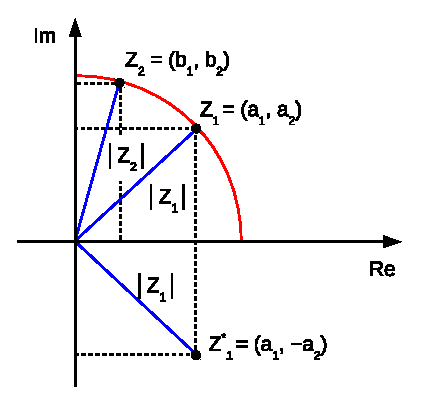
\includegraphics[scale=1]{KomplexniRovina.eps}
\caption[Komplexní rovina]{Znázornění komplexní roviny s~vyznačením komplexních čísel. Dále jsou demonstrovány základní operace s~komplexními čísly -- komplexní sdružení a~absolutní hodnota (modul) komplexního čísla.}
\label{obr:RovinaKomplexnichCisel}
\end{figure}

Protože komplexní čísla tvoří komplexní rovinu, není možné je uspořádat podobně jako reálná čísla. Pro porovnávání komplexních čísel je možné zavést absolutní hodnotu komplexního čísla (modul) vztahem
\begin{equation}
|Z| = \sqrt{a_1^2 + a_2^2} \, \mbox{.}
\label{rov:AbsolutniHodnotaKomplex}
\end{equation}
Absolutní hodnota komplexního čísla je reálné nezáporné číslo a platí, že $|Z| = 0$ právě tehdy, když $Z = 0$. Komplexní čísla, která mají stejnou absolutní hodnotu, leží na kružnici o~poloměru $r = |Z|$ s~počátkem ve středu souřadného systému (v~obrázku \ref{obr:RovinaKomplexnichCisel} vyznačena červeně).

Pro komplexní čísla definujeme stejně jako pro čísla reálná tyto operace: sčítání, odčítání, násobení a dělení. Všechny operace zde pro úplnost shrneme. Mějme dvě komplexní čísla $Z_1 = \nobreak a_1 + ia_2$ a $Z_2=b_1 + ib_2$ zapsaná pro jednoduchost v~algebraickém tvaru.
\begin{enumerate}
\item Při sčítání (odčítání) sčítáme (odčítáme) zvlášť reálnou část a zvlášť imaginární část komplexních čísel.
\begin{equation}
Z_1 \pm Z_2 = (a_1 + ia_2) \pm (b_1 + ib_2) = (a_1 \pm b_1) + i(a_2 \pm b_2)
\label{rov:ScitaniOdcitaniKomplex}
\end{equation}
\item Komplexní čísla násobíme stejně jako dvojčleny. Nesmíme ale zapomenout, že platí vztah $i^2 = -1$.
\begin{equation}
Z_1 \cdot Z_2 = (a_1 + ia_2) \cdot (b_1 + ib_2) = (a_1b_1 - a_2b_2) + i(a_1b_2 + a_2b_1)
\label{rov:NasobeniKomplex}
\end{equation}
\item Dělíme tak, že podíl nejprve rozšíříme vhodnou jedničkou, abychom ve jmenovateli dostali reálné číslo. I~v~oboru komplexních čísel platí, že $b \not = 0$, jinak podíl není definován.
\begin{equation}
\frac{Z_1}{Z_2} = \frac{a_1 + ia_2}{b_1 + ib_2} = \frac{a_1 + ia_2}{b_1 + ib_2} \cdot \frac{b_1 - ib_2}{b_1 - ib_2} = \frac{(a_1b_1 + a_2b_2) + i(a_2b_1 - a_1b_2)}{b_1^2 + b_2^2}
\label{rov:DeleniKomplex}
\end{equation} 
\end{enumerate}

Při počítání s~komplexními čísly je výhodné definovat číslo komplexně sdružené ke komplexnímu číslu $Z$ vztahem
\begin{equation}
Z^\ast = (a_1, a_2)^\ast = (a_1, -a_2) \mbox{,}
\label{rov:KomplexSdruzCislo-uspdvoj}
\end{equation}
nebo podobně v~algebraickém tvaru
\begin{equation}
Z^\ast = (a_1 + ia_2)^\ast = a_1 - ia_2 \mbox{.}
\end{equation}
Geometrická interpretace komplexního sdružení je následující. Komplexně sdružené číslo $Z^\ast$ je osově souměrné ke komplexnímu číslu $Z$ podle osy reálných čísel $\mathbf{Re}$. Na obrázku~\ref{obr:RovinaKomplexnichCisel} je komplexně sdruženo číslo $Z_1$. Vynásobíme-li komplexní číslo s~číslem k~němu komplexně sdruženým, dostaneme kvadrát absolutní hodnoty komplexního čísla, protože
\begin{displaymath}
Z \cdot Z^\ast = (a_1, a_2) \cdot (a_1, a_2)^\ast = (a_1, a_2) \cdot (a_1, -a_2) = (a_1^2 + a_2^2, a_1a_2 - a_1a_2) = (a_1^2 + a_2^2, 0) = |Z|^2 \mbox{,}
\end{displaymath}
\begin{equation}
Z \cdot Z^\ast = |Z|^2 \mbox{.}
\label{rov:KvadradAbsolutniHodnoty}
\end{equation}

Pro sčítání a násobení komplexních čísel platí asociativní, komutativní a distributivní zákon podobně jako u~čísel reálných. Pro komplexně sdružená čísla je možné odvodit následující relace
\begin{equation}
(Z_1 + Z_2)^\ast = Z_1^\ast + Z_2^\ast \mbox{,} \quad (Z_1Z_2)^\ast = Z_1^\ast \cdot Z_2^\ast \mbox{,} \quad \left(\frac{Z_1}{Z_2}\right)^\ast = \frac{Z_2^\ast}{Z_2^\ast} \,\mbox{.}
\label{rov:OperaceSdruzCisla}
\end{equation}

Pro řadu výpočetních aplikací je výhodné komplexní číslo $Z$ zapsat v~tzv. goniometrickém tvaru. Ten odvodíme tak, že v~komplexní rovině zobrazíme komplexní číslo $Z$ a uděláme pravoúhlé průměty absolutní hodnoty komplexního čísla $|Z|$ do reálné $\mathbf{Re}$ a imaginární $\mathbf{Im}$ osy. Označíme-li orientovaný úhel, který svírá průvodič absolutní hodnoty s~osou reálných čísel jako $\theta$, můžeme odvodit, že 
\begin{equation}
a_1 = |Z| \cos \theta \mbox{,} \quad a_2 = |Z| \sin \theta \mbox{.}
\label{rov:PrumetyKomplexnihoCisla}
\end{equation}
Dosadíme-li průměty $a_1$ a $a_2$ z~rovnice (\ref{rov:PrumetyKomplexnihoCisla}) do algebraického tvaru komplexního čísla $Z = a_1 + ia_2$, pak po drobných úpravách odvodíme goniometrický tvar komplexního čísla
\begin{displaymath}
Z = a_1 + ia_2 = |Z| \cos \theta + i (|Z| \sin \theta)
\end{displaymath}
\begin{equation}
Z = |Z| (\cos \theta + i\sin \theta) \mbox{.}
\label{rov:KomplexniCisloGoniomTvar}
\end{equation}
Pro větší názornost je odvození goniometrického tvaru komplexního čísla daného vztahem (\ref{rov:KomplexniCisloGoniomTvar}) graficky znázorněno na obrázku~\ref{obr:GoniometrickyTvar}.
\begin{figure} [ht]
\centering
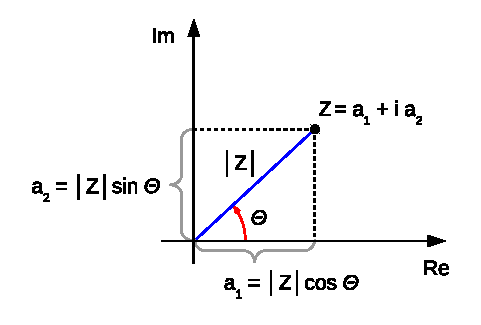
\includegraphics[scale=1]{GoniomTvar.eps}
\caption[Goniometrický tvar komplexního čísla]{K~odvození zápisu komplexního čísla v~goniometrickém tvaru.}
\label{obr:GoniometrickyTvar}
\end{figure}

V~kvantové mechanice se nám bude často hodit tzv. Eulerova identita
\begin{equation}
\boxed{e^{i \theta} = \cos \theta + i \sin \theta \mbox{,}}
\label{rov:EulerovaIdentita}
\end{equation}
která je základem komplexní analýzy, oboru matematiky studujícím funkce komplexní proměnné. Pro zájemce nyní dodáváme její odvození. Nejprve si připomeneme Taylorovu rozvoj funkce $e^{x}$ okolo bodu $x_0 = 0$. Hledaná Taylorova řada je
\begin{equation}
e^x = \sum_{n=0}^{\infty} \frac{x^n}{n!} \,\mbox{.}
\label{rov:TaylorovaRadaExponenciela}
\end{equation}
Pro další použití v~odvození si ještě připomeneme Taylorovy rozvoje funkcí $\sin x$ a $\cos x$
\begin{equation}
\sin x = \sum_{n=0}^{\infty} (-1)^{n} \frac{x^{2n+1}}{(2n+1)!} \mbox{,} \quad \cos x = \sum_{n=0}^{\infty} (-1)^{n} \frac{x^{2n}}{(2n)!} \mbox{.}
\label{rov:RadaCosinusSinus}
\end{equation}
Čistě formální záměnnou $x \equiv i \theta$ ve vztahu (\ref{rov:TaylorovaRadaExponenciela}) dostaneme po rozepsání Taylorovu řadu ve tvaru
\begin{equation}
e^{i\theta} = 1 + i\theta - \frac{\theta^2}{2!} - i \frac{\theta^3}{3!} + \frac{\theta^4}{4!} + i \frac{\theta^5}{5!} -\,\dots
\label{rov:RadaExponenciela1}
\end{equation}
Přeuspořádáním řady (\ref{rov:RadaExponenciela1}) a využitím vztahů (\ref{rov:RadaCosinusSinus}) dostaneme
\newpage
\begin{displaymath}
e^{i\theta} = 1 + i\theta - \frac{\theta^2}{2!} - i \frac{\theta^3}{3!} + \frac{\theta^4}{4!} + i \frac{\theta^5}{5!} -\,\dots =\underbrace{\left(1 - \frac{\theta^2}{2!} + \frac{\theta^4}{4!} - \,\dots \right)}_{\cos \theta} + i \underbrace{\left(x - \frac{\theta^3}{3!} + \frac{\theta^5}{5!} - \,\dots \right)}_{\sin \theta}
\end{displaymath}
\begin{equation}
e^{i\theta} = \cos \theta + i\sin \theta \mbox{,}
\label{rov:DukazEulerovaIdentita}
\end{equation}
což je Eulerova identita, kterou jsme chtěli odvodit. Eulerova identita umožňuje komplexní číslo $Z$ zapsat v~tzv. exponenciálním tvaru.

Exponenciální tvar komplexního čísla $Z$ odvodíme tak, že vyjdeme z~goniometrického tvaru komplexního čísla (\ref{rov:KomplexniCisloGoniomTvar}), do kterého dosadíme Eulerovu identitu (\ref{rov:EulerovaIdentita})
\begin{equation}
Z = |Z| e^{i \theta} \mbox{.}
\label{rov:ExponencialniTvar}
\end{equation}
Exponenciální tvar komplexního čísla je obzvlášť šikovný při násobení a dělení komplexních čísel. Pro násobení komplexních čísel $Z_1 = |Z_1| e^{i \theta}$ a $Z_2 = |Z_2|e^{i \phi}$ v~exponenciálním tvaru dostaneme
\begin{equation}
Z_1Z_2 = |Z_1| \cdot |Z_2| \cdot e^{i(\theta + \phi)} \mbox{.}
\label{rov:NasobeniExponencialniTvar} 
\end{equation}
Podobně pro dělení komplexních čísel $Z_1$ a $Z_2$ dostaneme
\begin{equation}
\frac{Z_1}{Z_2} = \frac{|Z_1|}{|Z_2|} \cdot e^{i(\theta - \phi)} \mbox{.}
\label{rov:DeleniExponencialniTvar}
\end{equation}

Zapíšeme-li komplexní číslo v~exponenciálním tvaru, je intuitivní definovat mocninu komplexního čísla $Z$. Pro počítání s~mocninami platí, že 
\begin{equation}
Z^n = |Z|^n e^{in\theta} \mbox{,}
\label{rov:MocninaKomplexnihoCisla}
\end{equation}
což je hledaná $n$-tá mocnina komplexního čísla $Z$. Dosazením Eulerovy identity (\ref{rov:EulerovaIdentita}) do rovnice (\ref{rov:MocninaKomplexnihoCisla}) můžeme odvodit známou Moivreovu větu
\begin{equation}
(e^{i\theta})^n = e^{i n \theta} \quad \mbox{tj.} \quad (\cos \theta + i \sin \theta )^n = \cos n\theta + i \sin n\theta \mbox{.}
\label{rov:MoivreovaVeta}
\end{equation}

Na závěr kapitoly o~komplexních číslech si ukážeme jeden ilustrační příklad, který demonstruje, jak odvozovat různé goniometrické identity pomocí Moivreovy věty.

\begin{priklad}
\textbf{Zadání:} Odvoďte známé vzorečky pro kosinus a sinus dvojnásobného argumentu
\begin{displaymath}
\cos 2\theta = \cos^2 \theta - \sin^2 \theta \quad \mbox{a} \quad
\sin 2\theta = 2 \sin \theta \cos \theta \mbox{.}
\end{displaymath}
\textbf{Řešení:} Použijeme Moivreovu větu (\ref{rov:MoivreovaVeta}) ve tvaru
\begin{displaymath}
(\cos \theta + i \sin \theta )^2 = \cos^2 \theta + 2 i \cos \theta \sin \theta - \sin^2 \theta = \cos 2 \theta + i \sin 2 \theta
\end{displaymath}
Odtud porovnáním členů s~a bez komplexní jednotky dostaneme vzorečky pro kosinus a sinus dvojnásobného argumentu.
\end{priklad}

\newpage

\subsection{Operátory}
\label{kap:Operatory}

\subsubsection{Co je operátor}

Čtenář je nepochybně intimně seznámen s~pojmem funkce. Funkce představuje matematickou operaci, kdy působením na číslo (nezávisle proměnnou) získáme nové číslo (závisle proměnnou). Operátor naproti tomu představuje matematickou operaci, kdy působením na funkci získáme funkci novou. Působením operátoru $\hat{O}$ na funkci $f$ zapíšeme
\begin{equation}
\boxed{\hat{O} f = g \mbox{,}}
\label{rov:Operator}
\end{equation}
kde výsledkem působení operátoru $\hat{O}$ je nová funkce $g$. Zapamatujme si, že z~definiční rovnice působení operátoru na funkci (\ref{rov:Operator}) plyne, že pořadí operátoru a funkce, na kterou operátor působí, není libovolné, ale že operátor vždy působí na funkci stojící napravo od operátoru.

Abychom se blíže seznámili s~operátory, představme si několik základních typů operátorů. Nejjednodušším operátorem může být operátor
\begin{equation}
\hat{O} = 1,
\nonumber
\end{equation}
neboli operátor identity nebo také jednotkový operátor. Tento operátor působě na libovolnou funkci $f$ vrátí funkci $g$ takovou, že platí $g=1 \cdot f$. Dalším jednoduchým operátorem může být například násobení proměnnou $x$
\begin{equation}
\hat{O} = x.
\nonumber
\end{equation}
Pakliže tento operátor bude působit na funkci $f = x^2$ dostaneme
\begin{equation}
\hat{O} f = x \cdot f = x \cdot x^2 = x^3 = g.
\nonumber
\end{equation}
Další důležitou třídou operátorů jsou diferenciální operátory, například
\begin{equation}
\hat{O} = \frac{\mathrm{d}}{\mathrm{d}x}.
\nonumber
\end{equation}
Vidíme, že derivaci funkce podle proměnné $x$ můžeme chápat jako působení operátoru derivace $\hat{O}$ na funkci $f(x)$. Názorný příklad působení diferenciálního operátoru uvádí příklad \ref{pr:Operator}.

\begin{priklad} \label{pr:Operator}
\textbf{Zadání:} Nalezněte výsledek působení operátoru $\hat{O}=\frac{\mathrm{d}}{\mathrm{d}x}$ na funkci $f(x) = \sin x$. \\
\textbf{Řešení:} Zapíšeme rovnici vyjadřující působení operátoru $\hat{O}$ na funkci $f(x)$ a dostaneme
\begin{displaymath}
\hat{O} f(x) = \frac{\mathrm{d}}{\mathrm{d}x} \sin x = \cos x \equiv g(x)
\end{displaymath}
Vidíme, že výsledkem působení operátoru $\hat{O}$ na funkci $f(x)$ je nová funkce $g(x) = \cos x$.
\end{priklad}

V~kvantové mechanice operátory reprezentující měřitelné veličiny, například pozici, hybnost, moment hybnosti nebo celkovou energii systému. V~kapitole \ref{kap:historie} o~historickém vývoji kvantové mechaniky jsme se seznámili se Schrödingerovou rovnicí popisující pohyb částice v~jedné dimenzi
\begin{equation}
\left( -\frac{\hbar^2}{2m}\frac{\mathrm{d}^2}{\mathrm{d} x^2} + V(x) \right) \Psi(x) = E \Psi(x) \mbox{,}
\label{rov:SCHR}
\end{equation}
Tuto rovnici můžeme přepsat jako operátorovou rovnici, tj. rovnici ve které vystupují operátory
\begin{equation}
\hat{H}\Psi(x) = E \Psi(x)\mbox{,}
\label{rov:SCHR-operator}
\end{equation}
kde $\hat{H}$ je operátor celkové energie systému, tzv. hamiltonián (Hamiltonův operátor). Porovnáním rovnice \eqref{rov:SCHR} s~rovnicí \eqref{rov:SCHR-operator} odvodíme předpis pro hamiltonián
\begin{equation}
\hat{H} \equiv \left( -\frac{\hbar^2}{2m}\frac{\mathrm{d}^2}{\mathrm{d} x^2} + V(x) \right)
\label{rov:Hamiltonian1D}
\end{equation}

V~obecném případě pohybu částice v~třírozměrném prostoru má Hamiltonův operátor tvar
\begin{equation}
\hat{H} \equiv \left( -\frac{\hbar^2}{2m}\Delta + V(x) \right) \mbox{,}
\label{rov:Hamiltonian3D}
\end{equation}
kde symbol $\Delta$ představuje Laplaceův operátor, který je druhou mocninou operátoru nabla $\Delta = \nabla^2$  a v~kartézských souřadnicích má tvar
\begin{equation}
\Delta = \frac{\partial^2}{\partial x^2}+\frac{\partial^2}{\partial y^2}+\frac{\partial^2}{\partial z^2} \mbox{.}
\label{rov:LaplaceuvOperator}
\end{equation}

Konkrétní tvar hamiltoniánu (\ref{rov:Hamiltonian3D}) závisí na konkrétní formě potenciální energie $V(x)$. Například v~případě vodíkového atomu, kdy se elektron pohybuje v~Coulombově poli generovaném protonem bude mít hamiltonián pro elektron tvar
\begin{equation}
\hat{H} \equiv \left( -\frac{\hbar^2}{2m_e}\Delta - \frac{1}{4 \pi \epsilon_0}\frac{e^2}{r} \right) \mbox{,}
\label{rov:HamiltonianVodik}
\end{equation}
kde $e$ je elementární náboj elektronu, $m_e$ je hmotnost elektronu, $\epsilon_0$ je permitivita vakua a $r$ je vzdálenost protonu a elektronu.

Další hojně se vyskytující operátory jsou operátor hybnosti a operátor polohy
\begin{equation}
\hat{p}= -i\hbar \nabla \mbox{,}
\label{rov:OperatorHybnosti}
\end{equation}
\begin{equation}
\hat{r} = \mathbf{r} \mbox{,}
\label{rov:OperatorPozice}
\end{equation}
kde $\mathbf{r}=(x,y,z)$ je polohový vektor v~3D eukleidovském prostoru. Operátory (\ref{rov:OperatorHybnosti}) a (\ref{rov:OperatorPozice}) jsou zapsané v~tzv. souřadnicové reprezentaci, kdy operátor souřadnice je zvolen jako prosté násobení danou souřadnicí.

Vraťme se ještě jednou k~rovnici \eqref{rov:SCHR-operator}, ta je totiž speciálním případem třídy rovnic označovaných jako vlastní problém. Mějme operátor $\hat{O}$ a obecnou funkci $f$, pak rovnice
\begin{equation}
\boxed{\hat{O} f = \lambda f}
\label{rov:VlastniProblem}
\end{equation}
se označuje jako \textbf{vlastní problém operátoru} $\hat{O}$. Funkci $f$ pak nazýváme \textbf{vlastní funkce} operátoru $\hat{O}$ s~vlastním číslem $\lambda$. Jinak řečeno vlastní funkce $f$ operátoru $\hat{O}$ je taková funkce, že působí-li na ni operátor $\hat{O}$, pak výsledkem tohoto působení je funkce $f$ vynásobená číslem $\lambda$. V~případě rovnice \eqref{rov:SCHR-operator} je vlastní funkcí operátoru $\hat{H}$ vlnová funkce $\Psi(x)$ s~vlastním číslem $E$, celková energie systému. Vlastní problém operátoru má ústřední postavení v~kvantové mechanice, protože řešení většiny úloh znamená hledání vlastních čísel a vlastních funkcí příslušného operátoru. 



\subsubsection{Operace s~operátory}
\label{kap:OperaceSOperatory}

Podobně jako funkce můžeme mezi sebou sčítat, násobit, dělit atd. definujeme tyto operace i~pro počítání s~operátory. Vyjdeme ze vztahu (\ref{rov:Operator}), který definuje působení operátoru na funkci $f$ a ve stručnosti si představíme základní operace s~operátory.

Součtem dvou operátorů budeme rozumět operátor
\begin{equation}
\hat{C} = \hat{A}+\hat{B}
\label{rov:SoucetOperatoru1}
\end{equation}
takový, že platí
\begin{equation}
\hat{C}f = (\hat{A}+\hat{B})f=\hat{A}f + \hat{B}f \mbox{,}
\label{rov:SoucetOperatoru2}
\end{equation}
kde $f$ je libovolná testovací funkce. Pod součinem operátorů budeme rozumět operátor
\begin{equation}
\hat{C} = \hat{A}\hat{B}
\label{rov:SoucinOperatoru1}
\end{equation}
takový, že platí
\begin{equation}
\hat{C}f = \hat{A}(\hat{B}f) \mbox{.}
\label{rov:SoucinOperatoru2}
\end{equation}
Stejně jako v~případě násobení čísel figuruje číslo $1$ jako jednotkový prvek vůči násobení, je i~v~případě operátorového počtu definován jednotkový prvek -- jednotkový operátor $\hat{1}$
\begin{equation}
\hat{1} f = f \mbox{.}
\label{rov:JednotkovyOperator}
\end{equation}

\noindent Pomocí definice násobení operátorů (\ref{rov:SoucinOperatoru1}) můžeme definovat druhá mocnina operátoru
\begin{equation}
\hat{A}^2 = \hat{A}\hat{A} \mbox{.}
\label{rov:KvadratOperatoru} 
\end{equation}
A~dále matematickou indukcí můžeme definovat $n$-tou mocninu operátoru
\begin{equation}
\hat{A}^n f = \hat{A} (\hat{A}^{n-1} f) \mbox{.}
\label{rov:MocninaOperatoru}
\end{equation}

Obecně platí, že násobení operátorů (\ref{rov:SoucinOperatoru1}) není komutativní, to znamená, že neplatí
\begin{equation}
\hat{A}\hat{B} = \hat{B}\hat{A} \mbox{.}
\label{rov:KomutativnostOperatoru}
\end{equation}
Abychom mohli vyšetřovat komutativnost operátorů, zavádí se nový operátor -- \textbf{komutátor}
\begin{equation}
\boxed{[\hat{A},\hat{B}] \equiv \hat{A}\hat{B}-\hat{B}\hat{A} \mbox{.}}
\label{rov:KomutatorOperatoru}
\end{equation}
Když je komutátor dvou operátorů roven nulovému operátoru ($\hat{0}f=0$)
\begin{equation}
[\hat{A},\hat{B}] = \hat{0} \mbox{,}
\label{rov:Komutator1}
\end{equation}
říkáme, že operátory $\hat{A}$ a $\hat{B}$ spolu komutují. Když se komutátor nerovná nulovému operátoru, operátory nekomutují.

Jako příklad vyšetřování komutátoru dvou operátorů si spočtěme komutátor mezi operátorem hybnosti \eqref{rov:OperatorHybnosti} a souřadnice \eqref{rov:OperatorPozice}. Dostaneme
\begin{equation}
[\hat{r},\hat{p}] = -i \hbar \mathbf{r} \nabla + i \hbar \nabla \mathbf{r} = i \hbar (\nabla \mathbf{r} - \mathbf{r} \nabla) = i \hbar,
\nonumber
\end{equation}
kde jsme využili identity z~vektorové analýzy $\nabla \mathbf{r} - \mathbf{r} \nabla = \hat{1}$. Abychom ukázali, že tato identita platí, představme si, že řešíme problém pouze v~jedné dimenzi a současně si povšimněme, že levá strana identity má tvar komutátoru dvou operátorů. Dále víme, že komutátor je také operátor, který můžeme nechat působit na libovolnou funkci $f$. Dostaneme
\begin{equation}
\frac{\partial x f}{\partial x} - x\frac{\partial f}{\partial x} = f + xf^{\prime} - xf^{\prime} = f,
\nonumber
\end{equation}
kde první derivace je derivací součinu dvou funkcí. Odstraněním testovací funkce $f$ dostaneme
\begin{equation}
\frac{\partial x }{\partial x} - x\frac{\partial }{\partial x} = \hat{1},
\nonumber
\end{equation}
což je vektorová identita, kterou jsme chtěli dokázat.

Jak jsme ukázali v~názorném příkladu, výsledkem komutátoru operátoru momentu hybnosti a souřadnice je operátor
\begin{equation}
\boxed{[\hat{r},\hat{p}] = i \hbar,}
\label{rov:KomutatorHybnostSouradnice}
\end{equation}
který se nerovná nulovému operátoru, proto můžeme shrnout, že operátor hybnosti nekomutuje s~operátorem souřadnice.

\begin{priklad} \label{pr:Komutator}
\textbf{Zadání:} Určete komutátor operátorů $\hat{A} = \partial/\partial x$ a $\hat{B} = \partial / \partial y$. \\
\textbf{Řešení:} Sestavíme komutátor $[\hat{A},\hat{B}]$ a necháme ho působit na testovací funkci $f=f(x,y)$. Dostaneme
\begin{displaymath}
[\hat{A},\hat{B}] f = \frac{\partial f}{\partial x} \frac{\partial f}{\partial y} - \frac{\partial f}{\partial y} \frac{\partial f}{\partial x} = \frac{\partial^2 f}{\partial x \partial y} - \frac{\partial^2 f}{\partial y \partial x} = \hat{0},
\end{displaymath}
kde poslední rovnost je splněna tehdy, když funkce $f$ má spojité všechny druhé parciální derivace.

Vidíme, že výsledkem působení komutátoru je nulový operátor, proto můžeme uzavřít, že operátory $\hat{A}$ a $\hat{B}$ spolu komutují.
\end{priklad}

Z~definice komutátoru (\ref{rov:KomutatorOperatoru}) vyplývají tři důležité vlastnosti komutátorů. První vlastností je \textbf{antisymetrie}
\begin{equation}
[\hat{A},\hat{B}] = -[\hat{B},\hat{A}],
\label{rov:VlastnostKomutatoru1}
\end{equation}
která se týká toho, že záleží na pořadí operátorů v~komutátoru. To souvisí s~tím, že operátory obecně nekomutují. Například platí
\begin{equation}
[\hat{r},\hat{p}]= i \hbar,
\nonumber
\end{equation}
ale
\begin{equation}
[\hat{p},\hat{r}]= - i \hbar.
\nonumber
\end{equation}
Druhou vlastností je \textbf{linearita} v~druhém argumentu
\begin{equation}
[\hat{A},\hat{B}+\hat{C}] = [\hat{A},\hat{B}] + [\hat{A},\hat{C}].
\label{rov:VlastnostKomutatoru2}
\end{equation}
Ta souvisí s~tím, že komutátor je lineární operátor (viz další kapitola \ref{kap:OperatorySpecifickychVlastnosti}). Třetí vlastnost
\begin{equation}
[\alpha \cdot \hat{A},\hat{B}] = \alpha \cdot [\hat{A},\hat{B}]
\label{rov:VlastnostKomutatoru3}
\end{equation}
souvisí s~tím, že číslo $\alpha$ můžeme z~komutátoru vytknout.

Na závěr této kapitoly uvedeme jedno důležité tvrzení. \textbf{Komutují-li spolu dva operátory, tj. $[\hat{A},\hat{B}]=\hat{0}$, pak nutně mají společné vlastní funkce $f$.} Tvrzení si dokážeme. Předpokládejme, že máme dva libovolné operátory $\hat{A}$ a $\hat{B}$, pro které platí
\begin{equation}
\hat{A} f = a f
\nonumber
\end{equation}
a
\begin{equation}
\hat{B} f = b f,
\nonumber
\end{equation}
neboli operátory mají stejnou vlastní funkci $f$. Pak můžeme psát
\begin{equation}
\hat{A}\hat{B} f = \hat{A} (b f) = a b f
\nonumber
\end{equation}
a 
\begin{equation}
\hat{B}\hat{A} f = \hat{B} (a f) = a b f,
\nonumber
\end{equation}
protože čísla $a$ a $b$ komutují vždy. Odečtením předchozích dvou rovnic dostaneme
\begin{equation}
\hat{A}\hat{B} f - \hat{B}\hat{A} f  = (\hat{A}\hat{B} - \hat{B}\hat{A} ) f = [\hat{A}, \hat{B}] f = 0,
\nonumber
\end{equation}
což je výsledek, který jsme chtěli ukázat. Důkaz tvrzení je tak proveden. \hfill {\footnotesize $\blacksquare$}

\subsubsection{Prostory funkcí a Hilbertův prostor}
\label{kap:ProstoryFunkci}

Matematické objekty jako funkce nebo operátory jsou definovány na určitém prostoru $\mathcal{V}$. Prostor je v~matematice definován jako množina prvků, s~kterými je možné provádět jisté operace. Ze základního kurzu matematiky znáte lineární vektorový prostor $\mathcal{V}$ s~dvěma operacemi, sčítáním $+$ a násobením číslem $\cdot$, kde prvky prostoru jsou vektory, neboli uspořádané $N$-tice čísel.

Omezme se nyní v~našich úvahách na lineární vektorový prostor $\mathbb{R}^3$, který můžeme chápat jako 3D eukleidovský prostor. Pak libovolný vektor $\mathbf{v} = (v_1, v_2, v_3)$ můžeme pravoúhle promítnout do tří souřadných os, neboli reprezentovat tento vektor pomocí souboru vektorů souřadných os $e_1 = (1, 0, 0)$, $e_2 = (0, 1, 0)$ a $e_3 = (0, 0, 1)$.

Abychom nalezli tuto reprezentaci, tj. byli schopni vektor $\mathbf{v}$ zapsat pomocí vektorů souřadných os, nejprve určíme velikost průmětu vektoru $\mathbf{v}$ do jednotlivých souřadných os. K~tomu nám poslouží skalární součin vektoru $\mathbf{v}$ s~vektory souřadných os
\begin{equation}
\braket{e_i|\mathbf{v}} = v_i,
\nonumber
\end{equation}
kde zvolená symbolika pro skalární součin má své opodstatnění, jak uvidíme později. Vektor $\mathbf{v}$ tak můžeme v~reprezentaci vektorů souřadných os zapsat jako
\begin{equation}
\mathbf{v} = \sum_{i=1}^{3} \braket{e_i|\mathbf{v}} e_i.
\label{rov:RozvojVektoruDoBaze}
\end{equation}
Vztah \eqref{rov:RozvojVektoruDoBaze} si zaslouží pár poznámek. Zaprvé si uvědomme, že výsledkem skalárního součinu $\braket{e_i|\mathbf{v}}$ je číslo. Za druhé vektor je prvek mající velikost i směr, ve vztahu \eqref{rov:RozvojVektoruDoBaze} se o~velikost \uv{stará} skalární součin a o~směr jednotkové vektory souřadných os.

Vidíme, že abychom vektor $\mathbf{v}$ \uv{zrekonstruovali} z~vektorů reprezentující osy souřadného systému, musí být tento soubor vektorů $\{e_i\}$ úplný. Tak například, kdyby chyběl vektor $e_2$, nikdy bychom nebyli schopni zreprodukovat složku $v_2$ vektoru $\mathbf{v}$. Došli jsme k~závěru, že úplný soubor vektorů $\{e_i\}$ umožňuje reprezentovat libovolný prvek z~daného prostoru.

Úplný soubor vektorů $\{e_i\}$ bývá zvykem označovat za bázi daného prostoru. Báze má několik základních vlastností:
\begin{enumerate}
\item počet prvků báze je roven dimenzi prostoru,
\item pro libovolné dva prvky báze platí $\braket{e_i|e_j} = 0$, tj. prvky jsou na sebe kolmé -- ortogonální.
\end{enumerate}

Obeznámeni s~lineárními vektorovými prostory můžeme přistoupit k~definici prostoru funkcí. Prostor funkcí je prostor prvků, kterými jsou funkce mající jisté vlastnosti. V~analogii s~vektorovými prostory i zde existuje úplný soubor funkcí, do kterého můžeme rozložit libovolnou funkci prostoru
\begin{equation}
f = \sum_i c_i \varphi_i,
\label{rov:RozvojDoBazeFunkci}
\end{equation}
kde funkce $\varphi_i$ tvoří úplný soubor funkcí $\{\varphi_i\}$ a $c_i$ jsou rozvojové koeficienty. Příkladem úplného souboru funkcí je například soubor $x, x^2, x^3, \dots, x^n$.

V~kvantové mechanice je ústředním funkčním prostorem Hilbertův prostor, jehož prvky jsou kvadraticky integrovatelné komplexní funkce  splňující
\begin{equation}
\boxed{\int_{-\infty}^{\infty} |f(x)|^2 \,\mathrm{d}x < \infty}
\label{rov:KvandarickaIntegrovatelnost}
\end{equation} 
a dále je na tomto prostoru definována další vlastnost, skalární součin dvou funkcí
\begin{equation}
\boxed{\braket{f|g} \equiv \int_{-\infty}^{\infty} f^{\ast}(x) g(x) \mathrm{d}x,}
\label{rov:SkalarniSoucinFci}
\end{equation}
kde $^{\ast}$ značí komplexně sdruženou funkci. Zápis skalárního součinu ve tvaru $\braket{f|g}$, kde symbol $\bra{f}$ označovaný jako bra-vektor znamená komplexně sdruženou funkci $f^{\ast}$, symbol $\ket{g}$ označovaný jako ket-vektor znamená funkci $g$ a celý uzavřený symbol neboli braket chápeme jako integraci součinu funkcí $f^{\ast}g$, pochází od britského teoretického fyzika P.\,A.\,M.\,Diraca. Tato tzv. braketová notace se v~kvantové mechanice hojně využívá pro svou eleganci a úsporné zkrácení zápisu, který by byl jinak velmi složitý. V našem textu se této notaci spíše vyhýbáme.



\subsubsection{Operátory specifických vlastností}
\label{kap:OperatorySpecifickychVlastnosti}

Kvantová mechanika pracuje výhradně s~lineárními operátory, aby byl splněn princip superpozice, tj. jsou-li $\psi_1$ a $\psi_2$ vlnové funkce daného systému, pak i funkce $\psi=c_1\psi_1+c_2\psi_2$, kde $c_1$ a $c_2$ jsou libovolná komplexní čísla, je vlnovou funkcí uvažovaného systému. Pro lineární operátory platí
\begin{equation}
\boxed{\hat{A} (\alpha f + \beta g) = \alpha\hat{A}f + \beta\hat{A}g \mbox{,}}
\label{rov:LinearitaOperatoru}
\end{equation}
kde $\alpha$ a $\beta$ jsou obecně komplexní čísla.

Nejdůležitější operátory kvantové mechaniky jsou tzv. Hermitovy operátory $\hat{H}$ definované tak, že působí stejně na obou stranách skalárního součinu \eqref{rov:SkalarniSoucinFci}
\begin{equation}
\boxed{\int f^{\ast} \hat{H} g \,\mathrm{d}x = \int g \hat{H}^{\ast} f^{\ast} \,\mathrm{d}x,}
\label{rov:DefiniceHermitovaOperatoru}
\end{equation}
což můžeme v~braketové notaci zapsat jako
\begin{equation}
\braket{\hat{H}f|g} = \braket{f|\hat{H}g} \mbox{.}
\nonumber
\end{equation}
Z~definiční rovnice \eqref{rov:DefiniceHermitovaOperatoru} Hermitova operátoru vyplývá, že
\begin{equation}
\hat{H}^{\ast} = \hat{H} \mbox{.}
\nonumber
\end{equation}
Skutečnost, že Hermitovy operátory působí stejně v~levé i v~pravé straně skalárního součinu, se často značí následovně
\begin{equation}
\braket{f|\hat{H}|g} \mbox{.}
\nonumber
\end{equation}
Centrální pozice Hermitova operátoru $\hat{H}$ říká, že je jen na nás, zda necháme operátor působit v~levé nebo pravé straně skalárního součinu.

Nyní se podíváme na několik základních vlastností hermitovských operátorů. První vlastností je, že vlastní čísla hermitovského operátoru jsou reálná
\begin{equation}
\boxed{h^\ast = h.}
\label{rov:RealnaVlastniCisla}
\end{equation}
Tuto vlastnost si dokážeme. Uvažujme vlastní problém hermitovského operátoru
\begin{equation}
\hat{H} \psi = h \psi.
\nonumber
\end{equation}
Postupujme tak, že nejprve vlastní problém komplexně sdružíme
\begin{equation}
\hat{H}^\ast \psi^\ast = h^\ast \psi^\ast.
\nonumber
\end{equation}
Nyní vynásobme zleva komplexně sdružený vlastní problém funkcí $\psi$ a vlastní problém funkcí $\psi^\ast$ a integrujme, dostaneme
\begin{equation}
\int \psi \hat{H}^\ast \psi^\ast \,\mathrm{d}x = h^\ast \int \psi \psi^\ast \,\mathrm{d}x  = h^\ast
\nonumber 
\end{equation}
a
\begin{equation}
\int \psi^\ast \hat{H} \psi \,\mathrm{d}x = h \int \psi^\ast \psi \,\mathrm{d}x  = h.
\nonumber 
\end{equation}
Protože je operátor $\hat{H}$ hermitovský, platí
\begin{equation}
\int \psi \hat{H}^\ast \psi^\ast \,\mathrm{d}x = \int \psi^\ast \hat{H} \psi \,\mathrm{d}x
\nonumber
\end{equation}
a po odečtení posledních rovnic dostaneme
\begin{equation}
\int \psi \hat{H}^\ast \psi^\ast \,\mathrm{d}x - \int \psi^\ast \hat{H} \psi \,\mathrm{d}x =0  = h^\ast - h,
\nonumber
\end{equation}
a tedy
\begin{equation}
h^\ast = h,
\nonumber
\end{equation}
což jsme chtěli dokázat. \hfill {\footnotesize $\blacksquare$}

Dále ukážeme, že vlastní funkce hermitovského operátoru příslušející různým vlastním číslům jsou ortogonální, tj.
\begin{equation}
\boxed{\int_{-\infty}^{\infty} f_j^\ast f_i \,\mathrm{d}x = \delta_{ij},}
\label{rov:OrtogonalniVlastniFunkce}
\end{equation}
kde symbol $\delta_{ij}$ značí Kroneckerovo delta, které nabývá hodnoty $1$, když $i=j$ a hodnoty $0$, když $i \not = j$. Pomocí braketové symboliky můžeme vztah \eqref{rov:OrtogonalniVlastniFunkce} zapsat ve tvaru
\begin{equation}
\braket{f_i|f_j} = \delta_{ij}.
\nonumber
\end{equation}
Opět si tvrzení dokážeme. Předpokládejme platnost vztahů
\begin{equation}
\hat{H} \psi_1 = h_1 \psi_1
\nonumber
\end{equation}
a
\begin{equation}
\hat{H} \psi_2 = h_2 \psi_2 \mbox{,}
\nonumber
\end{equation}
kde $h_1 \not = h_2$. První rovnici vynásobíme zleva $\psi_2^\ast$ a integrujeme, druhou rovnici vynásobíme zleva $\psi_1^\ast$ a integrujeme, dostaneme
\begin{equation}
\int \psi_2^\ast \hat{H} \psi_1 \,\mathrm{d}x  = h_1 \int \psi_2^\ast \psi_1 \,\mathrm{d}x
\nonumber
\end{equation}
a
\begin{equation}
\int \psi_1^\ast \hat{H} \psi_2 \,\mathrm{d}x  = h_2 \int \psi_1^\ast \psi_2 \,\mathrm{d}x.
\nonumber
\end{equation}
Dále komplexně sdružíme například první rovnici a rovnice odečteme
\begin{equation}
0 = (h_1 - h_2 ) \int \psi_1^\ast \psi_2 \,\mathrm{d}x.
\nonumber
\end{equation}
Při úpravách jsme využili toho, že operátor $\hat{H}$ je hermitovský a že hermitovské operátory mají reálná vlastní čísla. Protože podle našeho počátečního předpokladu platí $h_1 \not = h_2$ je zřejmé, že musí platit
\begin{equation}
\int \psi_1^\ast \psi_2 \,\mathrm{d}x = 0,
\nonumber
\end{equation}
což jsme chtěli ukázat. Důkaz je tak proveden. \hfill {\footnotesize $\blacksquare$}

Na závěr si uveďme bez důkazu poslední důležitou vlastnost hermitovských operátorů. Soubor vlastních funkcí hermitovského operátoru vytváří úplný soubor bázových funkcí daného Hilbertova prostoru. To znamená, že když platí
\begin{equation}
\hat{H} f_i = h_i f_i \quad \mbox{pro každé}\quad i,
\nonumber
\end{equation}
pak libovolnou funkci $\psi$, můžeme zapsat jako lineární kombinaci
\begin{equation}
\psi = \sum_{i} c_i f_i,
\nonumber
\end{equation}
kde $c_i$ jsou rozvojové koeficienty.



\subsubsection{Postuláty kvantové mechaniky a operátory}
\label{kap:PostulatyKvantoveMechaniky}

Kvantová mechanika, podobně jako klasická Newtonova mechanika, je založena na několika postulátech shrnutých v~kapitole \ref{kap:historie}. Obsahem druhého postulátu je tvrzení, že \textbf{každé fyzikální veličině, kterou můžeme pro danou částici naměřit, je přiřazen operátor, který působí na vlnovou funkci.} Přitom se předpokládá, že operátor je lineární a hermitovský. Hermicita operátoru je nezbytná z~hlediska měření fyzikálních veličin, protože podle třetího postulátu \textbf{jediné hodnoty, které může měřitelná fyzikální veličina $A$ při jednotlivých měřeních nabývat, jsou vlastní čísla $a_n$ odpovídajícího operátoru $\hat{A}$.}

Obsahem čtvrtého postulátu je střední hodnota měření veličiny $A$ na kvantově mechanickém souboru. \textbf{Je-li systém popsán v~okamžiku měření normovanou vlnovou funkcí $\psi$, pak výsledkem měření na odpovídajícím kvantově mechanickém souboru je střední hodnota veličiny $A$ daná vztahem}
\begin{equation}
\boxed{\bar{A} = \int \psi^\ast \hat{A} \psi \,\mathrm{d}x,}
\label{rov:StředniHodnotaVeliciny}
\end{equation}
kde integrace se provádí přes celý dostupný prostor. V~duchu braketové notace můžeme psát
\begin{equation}
\bar{A} = \braket{\psi|\hat{A}|\psi} \mbox{.}
\nonumber
\end{equation}

Jestliže vlnová funkce $\psi$ je vlastní funkcí hermitovského operátoru $\hat{A}$ s~vlastním číslem $a$~pak
\begin{equation}
\bar{A} = \int \psi^{\ast} \hat{A} \psi \,\mathrm{d}x = \int \psi^{\ast} a \psi \,\mathrm{d}x = a \int \psi^{\ast} \psi \,\mathrm{d}x.
\label{rov:MerenaHodnota1}
\end{equation}
Výsledek (\ref{rov:MerenaHodnota1}) můžeme interpretovat následovně. Připravíme-li systém tak, že je charakterizovaný vlnovou funkcí, která je vlastní funkcí příslušného operátoru $\hat{A}$, poskytne opakované měření veličiny příslušné k~operátoru $\hat{A}$ vždy stejnou hodnotu fyzikální veličiny -- vlastní číslo~$a$.

V~případě, že se nám nepodaří systém připravit tak, aby byl charakterizovaný vlastní funkcí příslušného operátoru, můžeme vlnovou funkci systému rozvinout do báze příslušného prostoru. Nechť $\psi$ je obecná vlnová funkce popisující systém. Vlnovou funkci $\psi$ můžeme rozvinout do vlastních funkcí daného hermitovského operátoru $\psi=\sum c_n \phi_n$, kde $\hat{A}\phi_n = a_n \phi_n$, které tvoří úplný soubor na daném Hilbertově prostoru. Pak pro střední hodnotu platí
\begin{eqnarray}
&\bar{A}&=\braket{\psi|\hat{A}|\psi}= \braket{\sum_m c_m \phi_m|\hat{A}|\sum_n c_n \phi_n}=\sum_{m,n} c_m^\ast c_n \braket{\phi_m|\hat{A}\phi_n} {}
\nonumber\\
& & {}= \sum_{m,n} c_m^\ast c_n \braket{\phi_m|a_n \phi_n} = \sum_{m,n} c_m^\ast c_n a_n \braket{\phi_m|\phi_n} \mbox{.}
\label{rov:MerenaHodnota2}
\end{eqnarray}
Protože vlastní funkce hermitovského operátoru jsou ortogonální (viz vztah \eqref{rov:OrtogonalniVlastniFunkce}) je skalární součin ve výrazu (\ref{rov:MerenaHodnota2}) nenulový pouze když $m=n$. Proto se dvojitá suma zredukuje na jednoduchou a výraz (\ref{rov:MerenaHodnota2}) přejde na jednoduchý tvar
\begin{equation}
\bar{A} = \sum_n c_n^\ast c_n a_n = \sum_n |c_n|^2 a_n \mbox{.}
\label{rov:MerenaHodnota3}
\end{equation}
Všimněme si výsledku, který jsme obdrželi. Střední hodnota veličiny na souboru popsaném vlnovou funkcí $\psi=\sum c_n \phi_n$ se počítá jako vážená suma vlastních čísel daného operátoru. Váhami jsou v~tomto případě kvadráty rozvojových koeficientů $|c_n|^2$, které mají význam pravděpodobnosti, že při měření na souboru naměříme právě hodnotu $a_n$.

Je to vztah (\ref{rov:MerenaHodnota3}), který z~kvantové mechaniky dělá pravděpodobnostní teorii. Protože pouze tehdy, když systém připravíme ve stavu, který odpovídá vlastní funkci příslušného operátoru, dostaneme při opakovaném měření té samé veličiny stejný výsledek, přesně podle vztahu (\ref{rov:MerenaHodnota1}). Ve všech ostatních případech můžeme pouze určit pravděpodobnost toho, že změříme danou hodnotu veličiny, která je určená kvadrátem rozvojových koeficientů vlnové funkce popisující systém do báze vlastních funkcí hermitovského operátoru.


\subsubsection{Maticová reprezentace operátorů}


Zabývejme se ještě na chvíli rozvojem libovolné funkce do báze daného prostoru, který je dán vztahem \eqref{rov:RozvojDoBazeFunkci}. A~pro jednoduchost zápisu adoptujme pro tuto chvíli braketovou notaci. Potom obecnou funkci $\ket{\psi}$ můžeme rozvinout do úplného souboru funkcí $\ket{\varphi_i}$
\begin{equation}
\ket{\psi} = \sum_i c_i \ket{\varphi_i} \mbox{.}
\nonumber
\end{equation}
Pak pro vlastní problém $\hat{A} \ket{\psi} = a \ket{\psi}$ můžeme psát
\begin{equation}
\sum_i c_i \hat{A} \ket{\varphi_i} = a \sum_i c_i \ket{\varphi_i} \mbox{.}
\nonumber
\end{equation}
Rovnici vynásobme zleva jednou konkrétní funkcí z~úplného souboru funkcí, například funkcí $\bra{\varphi_m}$
\begin{equation}
\sum_i c_i \braket{\varphi_m|\hat{A}|\varphi_i} = a \sum_i c_i \braket{\varphi_m|\varphi_i}= a c_m \mbox{,}
\label{rov:Matice4}
\end{equation}
kde jsme využili toho, že úplný soubor funkcí jsou vlastní funkce hermitovského operátoru, které jsou ortogonální, tj. skalární součin $\braket{s_m|s_i}$ je nenulový jenom v~případě, kdy $m=i$. Výsledkem je, že v~sumaci na pravé straně výrazu (\ref{rov:Matice4}) zůstane nenulový jen člen $a c_m$. Dále provedeme substituci
\begin{equation}
A_{mi} \equiv \braket{\varphi_m|\hat{A}|\varphi_i} \mbox{,}
\nonumber
\end{equation}
kde výraz $A_{mi}$ označujeme jako maticový element. Výsledkem je 
\begin{equation}
\sum_i A_{mi} \, c_i = a c_m \mbox{.}
\label{rov:Matice6}
\end{equation}
Rovnici (\ref{rov:Matice6}) můžeme zapsat pro $\forall m$ a výslednou soustavu $m$-rovnic zapíšeme jako maticovou rovnici
\begin{equation}
\boxed{\mathbb{A} \mathbf{c} = a \mathbf{c} \mbox{,}}
\label{rov:Matice7-vysledek}
\end{equation}
kde $\mathbb{A}$ je čtvercová matice $(m \times i)$ a $\mathbf{c}$ je sloupcový vektor rozvojových koeficientů.

Došli jsme k~důležitému závěru, který si zasluhuje bližší komentář. Pomocí postupu uvedeného výše jsme došli k~tomu, že řešení vlastního problému operátoru $\hat{A}$ se redukuje na počítání s~maticemi. Vzhledem k~tomu, že násobení matic je obecně nekomutativní, mají matice příhodné vlastnosti, aby byly vhodnou reprezentací operátorů. Toho si povšiml jako první německý fyzik Werner Heisenberg a formuloval svou interpretaci kvantové mechaniky, která vešla ve známost jako maticová mechanika.










\clearpage
\section{Základní úlohy kvantové mechaniky}
\label{kap:zakladniulohy}
V~této kapitole se podíváme na řešení Schrödingerovy rovnice pro některé jednoduché situace vedoucí k~analyticky řešitelným úlohám. Takových situací, které by byly zároveň fyzikálně zajímavé, není mnoho. Proto se při popisu složitějších problémů musíme uchýlit k~jistým zjednodušením a aproximacím, kterým se budeme blíže věnovat v~kapitole \ref{kap:pribliznemetody}.

Začneme s volnou částicí. Na tomto triviálním případě si vysvětlíme přístup k~řešení úloh pomocí časově nezávislé Schrödingerovy rovnice. Na volnou částici plynule navážeme popisem částice v~nekonečně hluboké potenciálové jámě. Zde si vysvětlíme odkud se bere kvantování energie a hybnosti. Na závěr kapitoly se ve stručnosti podíváme na velmi důležitý problém řešení kvantového harmonického oscilátoru, který slouží jako modelový fyzikální systém například pro vibrační pohyby molekul.

\subsection{Volná částice}
\label{kap:VolnaCastice}

Abychom názorně demonstrovali řešení časově nezávislé Schrödingerovy rovnice
\begin{equation}
(- \frac{\hbar^2}{2m} \Delta + V) \psi = \hat{H} \psi = E \psi \mbox{,}
\label{rov:SCHR-Tvar}
\end{equation}
začneme s~řešením nejjednoduššího možného problému, kterým je volná částice, tj. částice na kterou nepůsobí žádná síla, tj. $V = 0$. Protože volná částice se pohybuje volně, nejsou na řešení Schrödingerovy rovnice (\ref{rov:SCHR-Tvar}) kladeny žádné okrajové podmínky. Uvidíme, že neexistence okrajových podmínek vede k~tomu, že energie a hybnost částice nebudou kvantovány.

Pro jednoduchost budeme předpokládat, že částice se může pohybovat pouze v~jednom rozměru. Rovnice (\ref{rov:SCHR-Tvar}) pak přejde do tvaru
\begin{equation}
-\frac{\hbar^2}{2m} \frac{\mathrm{d}^2\psi(x)}{\mathrm{d}x^2} = E \psi(x) \mbox{,}
\label{rov:Volna1}
\end{equation}
kde jsme využili předpoklad, že částice je volná, tj. $V = 0$. Rovnici (\ref{rov:Volna1}) dále upravíme do tvaru
\begin{equation}
\left( \frac{\mathrm{d}^2}{\mathrm{d}x^2} + \frac{2mE}{\hbar^2} \right) \psi(x) = 0 \mbox{.}
\label{rov:Volna2}
\end{equation}
Protože celková energie volné částice je rovná kinetické energii částice $T=p^2/(2m)$ a protože kinetická energie může být kladná anebo nulová, můžeme pro celkovou energii volné částice psát $E \geq 0$. Vzhledem k~této nerovnosti můžeme zavést substituci
\begin{equation}
\frac{2mE}{\hbar^2} = k^2 \mbox{,}
\label{rov:Volna3}
\end{equation}
kde $k\geq0$ je reálné číslo, obvykle označované jako vlnový vektor. S~využitím substituce (\ref{rov:Volna3}) přejde rovnice (\ref{rov:Volna2}) do tvaru
\begin{equation}
\left( \frac{\mathrm{d}^2}{\mathrm{d}x^2} + k^2 \right) \psi(x) = 0 \mbox{,}
\label{rov:Volna4}
\end{equation}
což je obyčejná diferenciální rovnice s~konstantními koeficienty. Rovnice tohoto typu řešíme metodou charakteristického polynomu. V~tomto případě je příslušný charakteristický polynom
\begin{equation}
\lambda^2 + k^2 = 0 \mbox{.}
\label{rov:Volna5}
\end{equation}
Řešením dostaneme kořeny
\begin{equation}
\lambda_{1,2} = \pm ik \mbox{.}
\label{rov:Volna6}
\end{equation}
Podle předpokladu o~řešení můžeme zapsat homogenní řešení rovnice (\ref{rov:Volna4}) ve tvaru
\begin{equation}
\psi(x) = e^{\pm ikx} \mbox{.}
\label{rov:Volna7}
\end{equation}
Působením operátoru hybnosti  $\hat{p}$ na vlnovou funkci (\ref{rov:Volna7}) dostaneme
\begin{equation}
\hat{p} \psi(x) = -i\hbar \frac{\mathrm{d}\psi(x)}{\mathrm{d}x} = \pm \hbar k \psi(x) \mbox{.}
\label{rov:Volna8}
\end{equation}
Z~rovnosti (\ref{rov:Volna8}) vyplývají vlastní hodnoty hybnosti volné částice ve tvaru
\begin{equation}
p = \pm \hbar k \mbox{.}
\label{rov:Volna9}
\end{equation}
Vlnovou funkci volné částice proto můžeme zapsat jako
\begin{equation}
\boxed{\psi(x) = e^{-px/(i\hbar)} \mbox{.}}
\label{rov:Volna10}
\end{equation}
Vyjádříme-li celkovou energii částice pomocí hybnosti $p$, dostaneme výraz pro energii ve tvaru
\begin{equation}
\boxed{E = \frac{p^2}{2m} = \frac{\hbar^2k^2}{2m} \mbox{.}}
\label{rov:Volna11}
\end{equation}
Vidíme, že ani hybnost ani energie volné částice nejsou kvantovány.

Na závěr si shrňme výsledky, ke kterým jsme při odvození došli. Vlnová funkce pro volnou částici je vlastní funkcí hamiltoniánu
\begin{equation}
\hat{H} = \hat{T} = \frac{\hat{p}^2}{2m} = -\frac{\hbar^2}{2m}\frac{\mathrm{d}^2}{\mathrm{d}x^2}
\label{rov:Volna12}
\end{equation}
s~vlastní hodnotou neboli energií $E = p^2/(2m)$. Dále víme, že vlnová funkce volné částice je i~vlastní funkcí operátoru momentu hybnosti $\hat{p} = -i\hbar ({\mathrm{d}}/{\mathrm{d}x})$ s~vlastní hodnotou $p = \pm \hbar k$. Z~toho vyplývá, že komutátor operátorů
\begin{equation}
[\hat{T},\hat{p}]
\label{rov:Volna13}
\end{equation}
musí být roven nule. Protože operátory spolu komutují (komutátor je nulový), mají společný soubor vlastních vlnových funkcí, a tak lze jednorozměrný pohyb volné částice charakterizovat pomocí dvou kvantových čísel -- kinetické energie $E = p^2/(2m)$ a hybnosti $p$. Dále si všimněme, že de Broglieův vztah mezi vlnovým vektorem a hybností částice jsme zde nemuseli předpokládat, ale že nám vyšel z~řešení Schrödingerovy rovnice (\ref{rov:Volna1}) pro volnou částici.

\subsection{Částice v~nekonečně hluboké potenciálové jámě}
\label{kap:CasticeJama}

Problém částice v~nekonečně hluboké jámě nám poslouží jako vzorový příklad kvantověmechanického problému, ve kterém se okrajové podmínky kladené na řešení projeví v~kvantování energií a hybností. Uvažujme nejdříve pro jednoduchost jednorozměrný případ, který pak přirozeně rozšíříme na trojrozměrný případ.

Předpokládejme, že v~intervalu $\langle0,a\rangle$ je potenciální energie $V(x)$ rovna nule, tj. $V = 0$. Dále předpokládejme, že mimo tento interval je potenciální energie nekonečná, tj. $V \rightarrow \infty$. Tímto předpokladem jsme si vytvořili potenciální jámu, která je pro částici uvězněnou uvnitř jámy, tj. v~intervalu $\langle0,a\rangle$ neproniknutelná, protože částice nemůže mít nekonečnou hodnotu energie.

Pro vlnovou funkci částice mimo jámu platí
\begin{equation}
\psi(x) = 0
\label{rov:Jama1}
\end{equation}
pro $x$ takové, že $x < 0$ a $x< a$. Výraz (\ref{rov:Jama1}) je vyjádřením skutečnosti, že částice se mimo potenciálovou jámu nemůže vyskytovat. Když máme vyřešen problém mimo samotnou jámu, zbývá nám vyřešit pohyb částice v~jámě. Pro tento případ hledáme řešení Schrödingerovy rovnice
\begin{equation}
-\frac{\hbar^2}{2m} \frac{\mathrm{d}^2\psi(x)}{\mathrm{d}x^2} = E \psi(x)
\label{rov:Jama2}
\end{equation}
pro hodnoty $x$ takové, že $x\in\langle 0,a\rangle $.

Diferenciální rovnici (\ref{rov:Jama2}) řešíme pomocí charakteristického polynomu ve tvaru
\begin{equation}
\lambda^2 + \frac{2mE}{\hbar^2} = 0 \mbox{.}
\label{rov:Jama3}
\end{equation}
Vzhledem k~tomu, že celková energie částice v~jámě odpovídá její kinetické energii (v~jámě platí $V = 0$), musí pro celkovou energii platit $E\geq0$. Proto můžeme zavést stejné označení jako v~kapitole \ref{kap:VolnaCastice} rovnice (\ref{rov:Volna3}). Řešením dostaneme pro $\lambda$ stejný výsledek jako ve výrazu (\ref{rov:Volna6}). Obecné řešení rovnice (\ref{rov:Jama2}) můžeme tedy zapsat ve tvaru
\begin{equation}
\psi(x) = Ae^{ikx} + Be^{-ikx} \mbox{,}
\label{rov:Jama4}
\end{equation}
kde $A$ a $B$ jsou libovolné komplexní konstanty.

Jedním z~postulátů, které kladou podmínky na akceptovatelnost vlnové funkce, je postulát o~spojitosti vlnové funkce. Vzhledem k~tomu, že mimo interval $\langle0,a\rangle$ je vlnová funkce nulová (\ref{rov:Jama1}), musí řešení (\ref{rov:Jama4}) splňovat následující okrajové podmínky
\begin{equation}
\psi(0)=0
\label{rov:Jama5}
\end{equation}
a
\begin{equation}
\psi(a)=0 \mbox{.}
\label{rov:Jama6}
\end{equation}
První podmínku splníme tak, že položíme $A = -B$, tj. místo obecné vlnové funkce (\ref{rov:Jama4}) vezmeme jen funkci ve tvaru
\begin{equation}
\psi(x)=N \sin(kx) \mbox{,}
\label{rov:Jama7}
\end{equation}
kde $N$ je normovací konstanta. Využili jsme přitom Eulerovu identitu \eqref{rov:EulerovaIdentita}. Druhou podmínku (\ref{rov:Jama6}) splníme tak, že položíme
\begin{equation}
ka = \pi n, \quad n= 1,2,3, \dots \mbox{,}
\label{rov:Jama8}
\end{equation}
kde $n$ je přirozené číslo -- kvantové číslo. V~případě $n=0$ bychom obdrželi řešení $\psi(x)=0$, které nemá fyzikální význam, neboť částice by se na intervalu $\langle0,a\rangle$ vůbec nevyskytovala.

Jak jsme předeslali, v~případě omezeného pohybu, zde neproniknutelnou potenciálovou bariérou, dospějeme k~závěru, že energie i odpovídající vlnový vektor jsou kvantovány
\begin{equation}
k_n = \frac{\pi}{a}n \quad n=1,2,3, \dots \mbox{,}
\label{rov:Jama9}
\end{equation}
\begin{equation}
\boxed{E_n = \frac{\pi^2\hbar^2}{2ma^2}n^2, \quad n=1,2,3, \dots }
\label{rov:Jama10}
\end{equation}
a že kvantování vyplývá z~okrajových podmínek (\ref{rov:Jama5}) a (\ref{rov:Jama6}). Vlnové funkce příslušející energiím daným vztahem (\ref{rov:Jama10}) jsou
\begin{equation}
\boxed{\psi_n(x) = N \sin \frac{\pi n x}{a}, \quad n=1,2,3,\dots \mbox{.}}
\label{rov:Jama11}
\end{equation}

V~tento okamžik nám zbývá jediné, určit normovací konstantu $N$ ze vztahu (\ref{rov:Jama11}). Určíme ji tak, že požadujeme, aby se částice nacházela někde uvnitř jámy
\begin{equation}
\int_{x=0}^a |N|^2 \sin^2 \frac{\pi x n}{a} \mathrm{d}x = 1 \mbox{,}
\label{rov:Jama12}
\end{equation}
který integrací vyřešíme a obdržíme
\begin{equation}
N = \sqrt{\frac{2}{a}}e^{i\alpha} \mbox{,}
\label{rov:Jama13}
\end{equation}
kde $\alpha$ je libovolné reálné číslo. Vidíme, že vlnová funkce $\psi(x)$ je určená až na fázový faktor $exp(i\alpha)$, který se zpravidla volí roven jedné.

Diskutujme nyní dosažené výsledky. Energie $E_n$ stacionárních stavů (získali jsme je řešením časově nezávislé -- stacionární -- Schrödingerovy rovnice (\ref{rov:Jama2})) jsou větší než nula. Stav s~energií $E_n=0$ není pro jámu o~konečné šířce $a$ možný. Energetické spektrum, neboli soubor všech energií, je diskrétní a nedegenerované, tj. vlastnímu číslu (energii) přísluší jen jedna vlnová funkce. A~konečně, energie $E_n$ jsou úměrné kvadrátu kvantového čísla $n^2$.

Vlnové funkce $\psi_n(x)$ pro částici v~nekonečné potenciální 1D jámě jsou ortonormální
\begin{equation}
\int_0^a \psi_m^\ast(x) \psi_n(x) \mathrm{d}x = \delta_{mn} \mbox{,}
\label{rov:Jama14}
\end{equation}
kde $\delta_{mn}$ je Kroneckerův symbol, který se rovná jedné, pakliže $m=n$, když $m \not = n$ je roven nule. Výraz (\ref{rov:Jama14}) je jen jiným způsobem zápisu ortonormálnosti dvou funkcí. Vlnové funkce $\psi_n(x)$ dále tvoří úplnou bázi na příslušném Hilbertově prostoru. Počet uzlových bodů, tj. těch kde $\psi_n(x)=0$ je roven $n-1$.

Rozšíření na trojrozměrný problém je poměrně intuitivní. Uvažujme potenciální energii $V(x,y,z) = 0$ všude v~oblasti $0\leq x\leq a$, $0\leq y \leq b$ a $0\leq z \leq c$, kde $a, b, c$ jsou rozměry uvažované jámy. Mimo tuto oblast je potenciální energie nekonečná, $V \rightarrow \infty$.

Schrödingerova rovnice pro tento problém je
\begin{equation}
-\frac{\hbar^2}{2m} \left(\frac{\partial^2}{\partial x^2} + \frac{\partial^2}{\partial y^2} + \frac{\partial^2}{\partial z^2} \right) \psi(x,y,z) = E \psi(x,y,z)
\label{rov:Jama15}
\end{equation}
a její řešení je možné hledat ve tvaru (metoda separace proměnných) 
\begin{equation}
\psi(x,y,z) = \psi_x(x)\psi_y(y)\psi_z(z) \mbox{.}
\label{rov:Jama16}
\end{equation}
Dále předpokládáme, že celkovou energii můžeme vyjádřit jako součet
\begin{equation}
E = E_x + E_y + E_z \mbox{.}
\label{rov:Jama17}
\end{equation}
Obdobným postupem řešení popsaným pro 1D případ dospějeme k~výsledku, že vlnová funkce částice v~3D jámě je
\begin{equation}
\psi_{lmn}(x,y,z) = \sqrt{\frac{8}{abc}} \sin \frac{\pi xl}{a}\sin \frac{\pi ym}{b} \sin \frac{\pi zn}{c}, \quad l,m,n = 1,2,3, \dots
\label{rov:Jama18}
\end{equation}
a jí odpovídající energie
\begin{equation}
E_{lmn} = \frac{\pi^2\hbar^2}{2m} \left(\frac{l^2}{a^2} + \frac{m^2}{b^2} + \frac{n^2}{c^2} \right), \quad l,m,n = 1,2,3, \dots \mbox{.}
\label{rov:Jama19} 
\end{equation}

Na rozdíl od 1D přpadu jsou zde degenerované energetické hladiny. To znamená, že dané energii odpovídá několik lineárně nezávislých vlnových funkcí.

\subsection{Harmonický oscilátor}
\label{kap:HarmonickyOscilator}

Harmonický, nebo přesněji lineární harmonický oscilátor je jednou z~fyzikálně důležitých úloh, pro kterou lze najít analytické řešení Schrödingerovy rovnice. Důležitost lineárního harmonického oscilátoru (LHO) plyne z~toho, že jeho potenciální energie odpovídá prvním členům Taylorova rozvoje obecného potenciálu $V(x)$ v~okolí minima $x=x_0$
\begin{equation}
V(x) = V(x_0) + \left(\frac{\mathrm{d}V}{\mathrm{d}x} \right)_{x=x_0} (x-x_0) + \frac{1}{2} \left(\frac{\mathrm{d}^2V}{\mathrm{d}x^2} \right)_{x=x_0} (x-x_0)^2 + \dots \mbox{.}
\label{rov:LHO1}
\end{equation}
První derivace potenciálu je v~minimu rovna nule, navíc omezíme-li se pouze na rozvoj do druhého řádu a zvolíme-li vhodnou referenční hladinu, například odečtením hodnoty $V(x_0)$, vztah (\ref{rov:LHO1}) se zjednoduší do tvaru
\begin{equation}
V(x) = \frac{1}{2} \left(\frac{\mathrm{d}^2V}{\mathrm{d}x^2} \right)_{x=x_0} (x-x_0)^2 \mbox{,}
\label{rov:LHO2}
\end{equation}
který odpovídá potenciálu LHO. Podobným způsobem můžeme postupovat i v~případě více dimenzí nebo u~vícečásticových systémů.

Například vhodnou volbou tzv. normálních souřadnic můžeme popisovat pomocí systému nezávislých LHO vibrace víceatomových molekul. Na druhou stranu si musíme být vědomi jistých omezení tohoto modelu. Zásadním omezením je skutečnost, že při zvětšování souřadnice $x \rightarrow \infty$ roste síla $F = -\mathrm{d}V/ \mathrm{d}x$ nade všechny meze, což je nefyzikální závěr. U~reálných systémů dojde při překročení jisté mezní výchylky z~rovnovážné polohy k~disociaci systému, což vede k~požadavku, že při $x \rightarrow \infty$ musí potenciál nabývat konečné hodnoty.

Při řešení 1D LHO vyjdeme ze Schrödingerovy rovnice, kde za potenciální energii systému dosadíme potenciál LHO
\begin{equation}
\left( -\frac{\hbar^2}{2m}\frac{\mathrm{d}^2}{\mathrm{d}x^2} + \frac{1}{2}m\omega^2x^2 \right) \psi(x) = E\psi(x) \mbox{.}
\label{rov:LHO3}
\end{equation}
Schrödingerova rovnice (\ref{rov:LHO3}) je diferenciální rovnicí s~nelineárními koeficienty u~nulté derivace. Tento typ rovnice se řeší tak, že nejprve rovnici upravíme do tvaru
\begin{equation}
\frac{\mathrm{d}^2}{\mathrm{d}x^2} \psi(x) + \left( \frac{2mE}{\hbar^2} - \frac{m^2\omega^2}{\hbar^2} x^2 \right) \psi(x) = 0 \mbox{.}
\label{rov:LHO4}
\end{equation}
Rovnice ve tvaru (\ref{rov:LHO4}) se dále řeší zavedením bezrozměrných proměnných
\begin{equation}
\xi \equiv \sqrt{\frac{m \omega}{\hbar}} x
\label{rov:LHO5}
\end{equation}
a
\begin{equation}
\lambda \equiv \frac{2E}{\hbar \omega} \mbox{.}
\label{rov:LHO6}
\end{equation}
Rovnici (\ref{rov:LHO4}) tak přejde do bezrozměrného tvaru
\begin{equation}
\frac{\mathrm{d}^2 \psi(\xi)}{\mathrm{d}\xi^2} + (\lambda - \xi^2)\psi(\xi) = 0 \mbox{.}
\label{rov:LHO7}
\end{equation}
Při řešení se dále postupuje tak, že nejprve hledáme asymptotické řešení vlnové funkce $\psi$ pro $\xi \rightarrow \pm \infty$, kdy v~rovnici (\ref{rov:LHO7}) můžeme člen s~$\lambda$ zanedbat, protože ve srovnání s~ostatními členy je malý.  Výsledkem je asymptotické řešení ve tvaru
\begin{equation}
\psi(\xi) = A e^{-\xi^2/2} + B e^{\xi^2/2} \mbox{,}
\label{rov:LHO8}
\end{equation}
kde $A$ a $B$ jsou libovolné konstanty. Pro znaménko plus ve výrazu (\ref{rov:LHO8}) vlnová funkce diverguje a nelze ji normovat, proto se vlnová funkce $\psi(\xi)$ asymptoticky chová jako funkce
\begin{equation}
\psi(\xi) = A e^{-\xi^2/2} \mbox{,}
\label{rov:LHO9}
\end{equation}
a tak můžeme řešení rovnice (\ref{rov:LHO7}) hledat ve tvaru
\begin{equation}
\psi(\xi) = v(\xi)e^{-\xi^2/2} \mbox{,}
\label{rov:LHO10}
\end{equation}
kde $v(\xi)$ je zatím neurčená funkce. Dosadíme-li předpokládané řešení (\ref{rov:LHO10}) do rovnice (\ref{rov:LHO7}) dostaneme po malé úpravě diferenciální rovnici
\begin{equation}
v^{\prime\prime} - 2\xi v^{\prime} + (\lambda - 1)v = 0 \mbox{,}
\label{rov:LHO11}
\end{equation}
kde čárka naznačuje derivaci podle $\xi$. Diferenciální rovnice (\ref{rov:LHO11}) se řeší pomocí rozvoje hledané funkce v~mocninou řadu, kde nakonec dojdeme k~rekurentnímu vztahu mezi koeficienty řady. Aby funkce $v(\xi)$ pro $\xi \rightarrow \pm \infty$ nedivergovala, musí dosud neurčité $\lambda$ splňovat podmínku
\begin{equation}
\lambda = 2n + 1, \quad n=0,1,2, \dots \mbox{.}
\label{rov:LHO12}
\end{equation}
S~přihlédnutím ke vztahu (\ref{rov:LHO6}) dostaneme pro energií stacionárních stavů
\begin{equation}
\boxed{E_n = \hbar \omega (n+ 1/2), \quad n=0,1,2, \dots \mbox{.}}
\label{rov:LHO13}
\end{equation}
Vidíme, že kvantování energií je opět dáno okrajovými podmínkami kladenými na uvažovaný systém. Z~rovnice (\ref{rov:LHO13}) také plyne, že když za $n$ dosadíme $n=0$, neboli počítáme \textbf{energii nulové hladiny} LHO, dostaneme
\begin{equation}
E_0 = \frac{\hbar \omega}{2} \mbox{.}
\label{rov:LHO16}
\end{equation}
Energie základního stavu je tak nenulová. To je podstatný rozdíl oproti klasické fyzice, kde částice může mít nulovou energii v~minimu potenciální energie $V(x)$. Nenulovost energie úzce souvisí s~relacemi neurčitosti. Energie (\ref{rov:LHO16}) je někdy označována jako energie nulových kmitů a lze ji například ověřit v~případě kmitů krystalové mřížky, kde na rozdíl od klasické fyziky vlivem nenulovosti kmitů, nevymizí rozmazání difrakčního obrazce ani při snižování teploty k~absolutní nule $T \rightarrow 0$.

Provedeme-li zpětné dosazení všech použitých substitucí a provedeme-li normalizaci vlnové funkce, získáme vlnové funkce LHO ve tvaru
\begin{equation}
\phi_n(x)=\frac{1}{\sqrt{x_0}}\frac{1}{\sqrt{2^n n! \pi^{1/2}}}e^{-(x/x_0)^2/2}H_n(x/x_0), \quad n=0,1,2, \dots \mbox{,}
\label{rov:LHO14}
\end{equation}
kde funkce $H_n(\xi)$ je funkce $v(\xi)$ ze vztahu (\ref{rov:LHO10}) a nazýváme je Hermitovy polynomy
\begin{equation}
H_n(\xi) = (-1)^n e^{\xi^2} \frac{\mathrm{d}^n}{\mathrm{d}\xi^n}e^{-\xi^2} \mbox{.}
\label{rov:LHO15}
\end{equation}

\begin{priklad}
\textbf{Zadání:} Molekula HCl silně absorbuje v infračervené oblasti spektra u $2991$~cm$^{-1}$. Spočtěte silovou konstantu $k$ pro tuto molekulu.\\[0.1cm]
\textbf{Řešení:} Zapíšeme $\Delta E = h \nu = h c / \lambda = \hbar \sqrt{k/\mu}$ a vyjádříme $k$
\begin{displaymath}
k = 4 \pi^2 \left( \frac{c}{\lambda} \right)^2 \mu = 516{,}3 \mbox{ N m}^{-1}.
\end{displaymath} \vspace{-0.7cm}
\end{priklad}



\clearpage
\section{Moment hybnosti}
\label{kap:momenthybnosti}
\newcounter{Odvozeni}

Momentem hybnosti na první pohled nepůsobí jako téma, které by bylo pro chemika obzvláště palčivé. Ve skutečnosti je ale z~kvantové teorie pro chemika málo co důležitějšího. V~této kapitole se budeme zabývat výhradně orbitálním moment hybnosti~$\mathbf{L}$, spin  odsuneme do kapitoly \ref{kap:elektronovyspin}.  

Povídání o~momentu hybnosti začneme jeho definicí z~klasické mechaniky. Vybaveni aparátem základních kvantově mechanických operátorů -- polohy a hybnosti, odvodíme operátory pro moment hybnosti a komutační relace mezi nimi. Ukážeme, že když operátory komutují, znamená to, že mají společné vlastní funkce. Toho dále využijeme při řešení vlastního problému operátorů momentu hybnosti.

Pro popis rotačního pohybu nejsou příliš vhodné kartézské souřadnice. Zavedeme si proto vhodnější souřadné systémy a ukážeme, jaké výhody při řešení problémů s~momentem hybnosti poskytují. 

\subsection{Operátor momentu hybnosti}
\label{kap:OperatorMomentuHybnosti}

Z~klasické fyziky víme, že pohybující se částice o~hmotnosti $m$ rychlostí $v$ nese hybnost
\begin{equation}
p = mv \mbox{.}
\label{rov:Hybnost1}
\end{equation}
Rotace částice je spojena s~momentem hybnosti
\begin{equation}
\mathbf{L} = \mathbf{r} \times \mathbf{p} \mbox{,}
\label{rov:Hybnost2}
\end{equation}
kde $\mathbf{r}$ je pozice částice vůči zvolenému počátku. Znaménko $\times$ znamená vektorový součin. Vektor momentu hybnosti pak můžeme zapsat ve formě
\begin{equation}
\mathbf{L} = \left\vert
\begin{array}[c]{ccc}
\mathbf{i}&\mathbf{j}&\mathbf{k}\\
x&y&z\\
p_x&p_y&p_z\\
\end{array} \right\vert
\mbox{,}
\label{rov:Hybnost3}
\end{equation}
kde $\mathbf{i}$, $\mathbf{j}$ a $\mathbf{k}$ jsou jednotkové vektory ve směru os x, y a z. 

Při odvození kvantově mechanického operátoru momentu hybnosti, vyjdeme z~toho, že moment hybnosti $\mathbf{L}$ je vyjádřen pomocí pozice $\mathbf{r}$ a hybnosti $\mathbf{p}$, pro které známe příslušné operátory (viz vztahy (\ref{rov:OperatorPozice}) a (\ref{rov:OperatorHybnosti}) v~kapitole \ref{kap:matematika})
\begin{equation}
\hat{p} = -i \hbar \nabla \quad \mbox{a} \quad \hat{r}=\mathbf{r} \mbox{.}
\label{rov:Hybnost4}
\end{equation}
Dosazením operátorů (\ref{rov:Hybnost4}) do definičního vztahu momentu hybnosti (\ref{rov:Hybnost2}) získáme operátor hybnosti
\begin{equation}
\boxed{\hat{L}= -i \hbar (\mathbf{r} \times \nabla) \mbox{.}}
\label{rov:Hybnost5}
\end{equation}
Pro jeho složky plyne z~(\ref{rov:Hybnost3})
\begin{equation}
\hat{L_x}=\hat{y}\hat{p_z}-\hat{z}\hat{p_y} = -i\hbar \left( y \frac{\partial}{\partial z} - z \frac{\partial}{\partial y} \right) \mbox{,}
\label{rov:Hybnost6}
\end{equation}
\begin{equation}
\hat{L_y}=\hat{z}\hat{p_x}-\hat{x}\hat{p_z} = -i\hbar \left( z \frac{\partial}{\partial x} - x \frac{\partial}{\partial z} \right) \mbox{,}
\label{rov:Hybnost7}
\end{equation}
\begin{equation}
\hat{L_z}=\hat{x}\hat{p_y}-\hat{y}\hat{p_x} = -i\hbar \left( x \frac{\partial}{\partial y} - y \frac{\partial}{\partial x} \right) \mbox{.}
\label{rov:Hybnost8}
\end{equation}

Při odvození komutačních relací mezi složkami momentu hybnosti vyjdeme ze základní komutační relace mezi pozicí a hybností
\begin{equation}
[q,p_q] = i \hbar \quad \mbox{a} \quad [q,p_n]=\hat{0}, \, q\not = n \mbox{,}
\label{rov:Hybnost9}
\end{equation}
kde $q$ i $n$ značí libovolnou složku kartézského prostoru. S~využitím vztahů (\ref{rov:Hybnost9}) odvodíme komutační relace mezi složkami momentu hybnosti
\begin{equation}
[L_x,L_y] = i\hbar \hat{L_z}, \quad [L_y,L_z] = i\hbar \hat{L_x}, \quad [L_z,L_x] = i\hbar \hat{L_y} \mbox{.}
\label{rov:Hybnost10}
\end{equation}

Protože je moment hybnosti vektor, můžeme definovat, jako u~každého vektoru, jeho velikost. V~kvantové mechanice je užitečné pracovat s~kvadrátem velikosti. Definujme kvadrát operátoru momentu hybnosti
\begin{equation}
\hat{L^2} = \hat{L_x^2}+\hat{L_y^2}+\hat{L_z^2}
\label{rov:Hybnost11}
\end{equation}
a odvoďme komutační relace mezi kvadrátem momentu hybnosti a složkami momentu hybnosti. Protože platí
\begin{equation}
[\hat{A^2},\hat{B}] = [\hat{A},\hat{B}]\hat{A} + \hat{A}[\hat{A},\hat{B}] \mbox{,}
\label{rov:Hybnost12}
\end{equation}
můžeme například pro $z$-ovou složku momentu hybnosti psát
\begin{eqnarray}
&[\hat{L^2}, \hat{L_z}]& = [\hat{L_x^2}+\hat{L_y^2}+\hat{L_z^2}, \hat{L_z}] \stackrel{a}{=} [\hat{L_x^2},\hat{L_z}] + [\hat{L_y^2},\hat{L_z}] + [\hat{L_z^2},\hat{L_z}] = {}
\nonumber\\
&& {}\stackrel{b}{=} [\hat{L_x},\hat{L_z}]\hat{L_x} + \hat{L_x}[\hat{L_x},\hat{L_z}] + [\hat{L_y},\hat{L_z}]\hat{L_y} + \hat{L_y}[\hat{L_y},\hat{L_z}] + \hat{0} = {}
\nonumber\\
&& {} \stackrel{c}{=} -i\hbar \hat{L_y}\hat{L_x} -i\hbar \hat{L_x}\hat{L_y} + i\hbar \hat{L_x}\hat{L_y} + i\hbar \hat{L_y}\hat{L_x} = \hat{0} \mbox{.}
\label{rov:Hybnost13}
\end{eqnarray}
Úprava označená jako $a$ plyne z~toho, že komutátor je lineární v~první argumentu. Úprava $b$ vychází ze vztahu (\ref{rov:Hybnost12}) a dále z~toho, že $ [\hat{L_z^2},\hat{L_z}]=\hat{0}$, protože operátor komutuje sám se sebou vždy. Úprava $c$ je dosazením z~dříve odvozených komutačních relací (\ref{rov:Hybnost10}). Analogicky jako pro $z$-ovou složku můžeme komutační relace odvodit i pro ostatní složky
\begin{equation}
\boxed{[\hat{L^2}, \hat{L_x}] = [\hat{L^2}, \hat{L_y}] = [\hat{L^2}, \hat{L_z}] = \hat{0} \mbox{.}}
\label{rov:Hybnost14}
\end{equation}
Vztah (\ref{rov:Hybnost14}) má zásadní důležitost, určuje maximální možnou informaci, kterou můžeme získat při měření momentu hybnosti kvantové částice, tedy současně můžeme změřit pouze kvadrát velikosti vektoru momentu hybnosti a jednu jeho složku, konvenčně se volí $z$-ová složka.

\subsection{Vlastní čísla operátorů momentu hybnosti}
\label{kap:VlastniCislaMomentHybnosti}

V~kapitole \ref{kap:PostulatyKvantoveMechaniky} jsme uvedli jeden z~postulátů kvantové mechaniky, že měřením dané veličiny získáme vlastní čísla příslušná operátoru, který zastupuje měřenou veličinu. Proto výsledkem měření momentu hybnosti budou vlastní čísla operátoru momentu hybnosti. Vztah \eqref{rov:Hybnost14} nám říká, že současně můžeme změřit kvadrát velikosti momentu hybnosti a jeho $z$-ovou složku. Protože vlastní čísla operátorů jsou určená rovnicí vlastního problému, zapíšeme si příslušné vlastí problémy těchto dvou operátorů
\begin{equation}
\hat{L^2} Y = c Y
\nonumber
\end{equation}
a
\begin{equation}
\hat{L_z} Y = b Y,
\nonumber
\end{equation}
kde $Y$ je společná vlastní funkce operátorů $\hat{L^2}$ a $\hat{L_z}$, protože z~kapitoly \ref{kap:OperaceSOperatory} víme, že když dva operátory komutují, mají společný soubor vlastních funkcí, $b$ a $c$ jsou vlastní čísla příslušných operátorů. V~odvození níže ukážeme, že vlastní čísla operátoru kvadrátu momentu hybnosti jsou
\begin{equation}
c = \hbar ^2 l(l+1) \quad \mbox{kde} \quad l = 0, 1, 2, \dots
\label{rov:VlastniCislaKvadratu}
\end{equation}
a vlastní čísla operátoru $z$-ové složky momentu hybnosti jsou
\begin{equation}
b = \hbar m \quad \mbox{kde} \quad m = 0, \pm 1, \pm 2, \dots, \pm l.
\label{rov:VlastniCislaZSlozky}
\end{equation}
Vidíme, že vlastní čísla, tj. měřitelné hodnoty, nemohou být libovolné, ale nabývají konkrétních diskrétních hodnot. Říkáme, že moment hybnosti je kvantován. Působení operátorů momentu hybnosti na vlnovou funkci můžeme zapsat jako
\begin{equation}
\boxed{\hat{L^2} = \hbar ^2 l(l+1)} \quad \mbox{kde} \quad l = 0, 1, 2, \dots
\label{rov:VlastniProblemKvadratu}
\end{equation}
a
\begin{equation}
\boxed{\hat{L_z} = \hbar m} \quad \mbox{kde} \quad m = 0, \pm 1, \pm 2, \dots, \pm l.
\label{rov:VlastniProblemZslozka}
\end{equation}

%odvozeni vztahu pro vlastni cisla operatoru momentu hybnosti
Pro zájemce nyní odvodíme relace \eqref{rov:VlastniProblemKvadratu} a \eqref{rov:VlastniProblemZslozka}. Vraťme se zpět k~rovnici (\ref{rov:Hybnost14}) a zapišme si vlastní problémy příslušných operátorů
\begin{equation}
\hat{L^2} Y_l^m = \lambda_l Y_l^m
\tag{O-\theOdvozeni}\stepcounter{Odvozeni}
\label{rov:Odvozeni1}
\end{equation}
a
\begin{equation}
\hat{L_z}Y_l^m = m Y_l^m \mbox{,}
\tag{O-\theOdvozeni}\stepcounter{Odvozeni}
\label{rov:Odvozeni2}
\end{equation}
kde $Y_l^m$ je vlastní funkce operátorů $\hat{L^2}$ a~$\hat{L_z}$. Abychom si při odvození usnadnili zápis vztahů, předpokládáme, že pracujeme v~takové soustavě jednotek, kde můžeme položit $\hbar=1$.

Naším cílem je odvodit výrazy pro vlastní čísla $\lambda_l$ a $m$. Zaveďme nový operátor $\hat{L_x^2} + \hat{L_y^2} = \hat{L^2}-\hat{L_z^2}$, který vznikne přepsáním operátoru kvadrátu momentu hybnosti (\ref{rov:Hybnost11}). Pak s~využitím vztahů \eqref{rov:Odvozeni1} a \eqref{rov:Odvozeni2} dostaneme
\begin{equation}
(\hat{L_x^2} + \hat{L_y^2}) Y_l^m = (\lambda_l - m^2) Y_l^m \mbox{.}
\tag{O-\theOdvozeni}\stepcounter{Odvozeni}
\label{rov:Odvozeni3}
\end{equation}
Protože vlastní čísla hermitovského operátoru jsou reálná (viz kapitola \ref{kap:matematika}) a protože kvadrát reálného čísla je číslo větší nebo rovno nule, můžeme ze vztahu \eqref{rov:Odvozeni3} vyvodit, že možné hodnoty $m$ jsou shora i zdola omezené, protože $m^2$ nemůže být větší než $\lambda_l$. Proto existuje minimální a~maximální hodnota $m$, které po řadě označíme jako $m_{min}$ a $m_{max}$.

Dále si definujme tzv. posuvné operátory
\begin{equation}
\hat{L_+} = \hat{L_x} + i \hat{L_y} \quad \mbox{a} \quad  \hat{L_-} = \hat{L_x} - i \hat{L_y} \mbox{.}
\tag{O-\theOdvozeni}\stepcounter{Odvozeni}
\label{rov:Odvozeni4}
\end{equation}
Aplikací rovnic (\ref{rov:Hybnost10}) a (\ref{rov:Hybnost14}) odvodíme příslušné komutační relace pro posuvné operátory ve tvaru
\begin{equation}
[\hat{L^2},\hat{L_{\pm}}]=\hat{0}, \quad [\hat{L_z},\hat{L_{\pm}}]=\pm L_{\pm} \mbox{.}
\tag{O-\theOdvozeni}\stepcounter{Odvozeni}
\label{rov:Odvozeni5}
\end{equation}


Necháme-li působit operátor $\hat{L_{\pm}}$ na stav $Y_l^m$ dostaneme
\begin{equation}
\hat{L^2}\hat{L_{\pm}} Y_l^m \stackrel {a}{=} \hat{L_{\pm}}\hat{L^2} Y_l^m = \lambda_l \hat{L_{\pm}} Y_l^m
\tag{O-\theOdvozeni}\stepcounter{Odvozeni}
\label{rov:Odvozeni6}
\end{equation}
a
\begin{equation}
\hat{L_z}\hat{L_{\pm}} Y_l^m \stackrel {b}{=} (\hat{L_{\pm}}\hat{L_z} \pm \hat{L_{\pm}})Y_l^m \stackrel{c}{=} (m \pm 1) \hat{L_{\pm}} Y_l^m \mbox{.}
\tag{O-\theOdvozeni}\stepcounter{Odvozeni}
\label{rov:Odvozeni7}
\end{equation}
Úprava $a$ vyplývá přímo z~příslušného komutátoru \eqref{rov:Odvozeni5}. Úprava $b$ vyplývá také z~příslušného komutátoru \eqref{rov:Odvozeni5}, ale již není tak přímočará. Komutátor je potřeba si rozepsat
\begin{equation}
[\hat{L_z},\hat{L_{\pm}}]= \hat{L_z}\hat{L_{\pm}} - \hat{L_{\pm}}\hat{L_z} = \pm L_{\pm} \mbox{.}
\tag{O-\theOdvozeni}\stepcounter{Odvozeni}
\label{rov:Odvozeni8}
\end{equation}
Šikovným přeuspořádáním komutátoru \eqref{rov:Odvozeni8} dostaneme úpravu $b$. Úpravu $c$ pro přehlednost rozepíšeme
\begin{equation}
(\hat{L_{\pm}}\hat{L_z} \pm \hat{L_{\pm}})Y_l^m = (\hat{L_{\pm}}\hat{L_z}) Y_l^m \pm \hat{L_{\pm}} Y_l^m = m\hat{L_{\pm}} Y_l^m \pm \hat{L_{\pm}} Y_l^m = (m \pm 1) \hat{L_{\pm}} Y_l^m \mbox{.}
\tag{O-\theOdvozeni}\stepcounter{Odvozeni}
\label{rov:Odvozeni9}
\end{equation}
Z~výrazu \eqref{rov:Odvozeni6} plyne, že $\hat{L_{\pm}} Y_l^m$ je vlastní funkcí operátoru $\hat{L^2}$ s~vlastním číslem $\lambda_l$. Ze vztahu \eqref{rov:Odvozeni7} obdobně dostaneme, že $\hat{L_{\pm}} Y_l^m$ je vlastní funkcí operátoru $\hat{L_z}$ s~vlastním číslem $m \pm 1$. Schopnost operátorů $\hat{L_{\pm}}$ měnit hodnotu $m$ o~$\pm 1$ jim dala jejich jméno -- posuvné.

Protože hodnota $m$ je ohraničená mezi $m_{min}$ a $m_{max}$ je logické, že
\begin{equation}
\hat{L_+} Y_l^{m_{max}} = 0
\tag{O-\theOdvozeni}\stepcounter{Odvozeni}
\label{rov:Odvozeni10}
\end{equation}
a
\begin{equation}
\hat{L_-} Y_l^{m_{min}} = 0 \mbox{,}
\tag{O-\theOdvozeni}\stepcounter{Odvozeni}
\label{rov:Odvozeni11}
\end{equation}
protože ani v~jednom případě není možné se posunout na vyšší/nižší hodnotu $m$ než je maximální/minimální hodnota. Z~rovnic \eqref{rov:Odvozeni10} a \eqref{rov:Odvozeni11} se můžeme vhodnou úpravou, rovnice vždy zleva vynásobíme druhým posuvným operátorem a využijeme identity $\hat{L_{\mp}}\hat{L_{\pm}} = \hat{L^2}-\hat{L_z}(\hat{L_z} \pm 1)$, dostat k~rovnicím
\begin{equation}
\lambda_l - m_{max}(m_{max}+1)=0 \quad \mbox{a} \quad \lambda_l - m_{min}(m_{min}-1)=0 \mbox{.}
\tag{O-\theOdvozeni}\stepcounter{Odvozeni}
\label{rov:Odvozeni12}
\end{equation}
Jejich spojením dostaneme rovnici
\begin{equation}
m_{max}^2 - m_{min}^2+m_{max}+m_{min}= 0 \mbox{.}
\tag{O-\theOdvozeni}\stepcounter{Odvozeni}
\label{rov:Odvozeni13}
\end{equation}
Rovnici řešme jako rovnici pro neznámou $m_{max}$. Výsledkem je $m_{max}=\{-m_{min};-1+m_{min}\}$. Protože $m_{max} \geq m_{min}$, je jediným řešením rovnice \eqref{rov:Odvozeni13}
\begin{equation}
m_{max} = -m_{min} \mbox{.}
\tag{O-\theOdvozeni}\stepcounter{Odvozeni}
\label{rov:Odvozeni14}
\end{equation}
Z~rovnice \eqref{rov:Odvozeni7} víme, že hodnoty $m$ se mění po jedničce. Proto $m_{max}-m_{min}$ musí být celé kladné číslo, což můžeme zapsat jako $2l$. Pak platí $m_{max}-m_{min} = 2l$ a $m_{max}+m_{min}=0$. Spojením těchto podmínek dostaneme
\begin{equation}
m_{max}=l, \quad m_{min}=-l \mbox{.}
\tag{O-\theOdvozeni}\stepcounter{Odvozeni}
\label{rov:Odvozeni15}
\end{equation}
Ze vztahů \eqref{rov:Odvozeni15} dále plyne, že existuje $2l+1$ možných hodnot $m$, $m=-l,\dots,0,\dots,+l$, pro každou hodnotu $l$. Když \eqref{rov:Odvozeni15} dosadíme do rovnice \eqref{rov:Odvozeni12}, odvodíme, že
\begin{equation}
\lambda_l = l(l+1)\mbox{.}
\tag{O-\theOdvozeni}\stepcounter{Odvozeni}
\label{rov:Odvozeni16}
\end{equation}
Když se vrátíme zpět ke klasické soustavě jednotek, tj. $\hbar \not = 1$, přejde výraz \eqref{rov:Odvozeni16} do tvaru
\begin{equation}
\lambda_l = l(l+1) \hbar^2,
\tag{O-\theOdvozeni}\stepcounter{Odvozeni}
\label{rov:Odvozeni17}
\end{equation}
což je výraz \eqref{rov:VlastniCislaKvadratu}, který jsme chtěli odvodit. \hfill {\footnotesize $\blacksquare$}
%konec odvozeni

Na závěr této kapitoly se zastavme u~toho, jak se komutační relace mezi operátory a~z~nich plynoucí současně měřitelné veličiny, projeví u~měření momentu hybnosti. Z~komutačních relací (\ref{rov:Hybnost10}) vidíme, že operátor $z$-ové složky momentu hybnosti nekomutuje se zbylými dvěma operátory složek momentu hybnosti. To znamená, že současně nemůžeme změřit všechny tři složky vektoru momentu hybnosti. Ale protože operátor $z$-ové složky momentu hybnosti komutuje s~operátorem kvadrátu momentu hybnosti (viz relace (\ref{rov:Hybnost14})), můžeme současně změřit  jednu složku, typicky $z$-ovou, vektoru momentu hybnosti a kvadrát velikosti vektoru momentu hybnosti. Grafická reprezentace výše uvedeného se označuje jako vektorový model momentu hybnosti $\mathbf{L}$. Vektorový model (obrázek~\ref{obr:VektorovyModel}) je vhodnou reprezentací prostorového kvantování, tj. faktu, že velikost a prostorová orientace vektoru momentu hybnosti nemůže být libovolná, ale nabývá diskrétních hodnot daných vlastními čísly operátorů $\hat{L^2}$ a $\hat{L_z}$.
\begin{figure} [!ht]
\centering
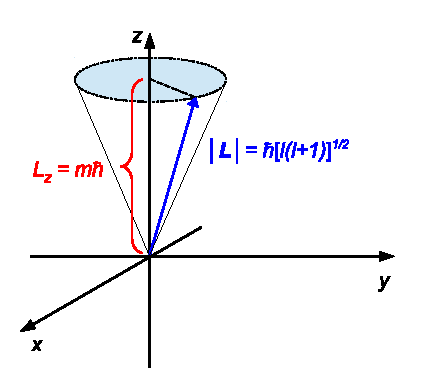
\includegraphics[scale=1]{vektorovymodel.eps}
\caption[Vektorový model momentu hybnosti]{Vektorový model momentu hybnosti. Protože jednotlivé složky vektoru momentu hybnosti spolu nekomutují, nemůžeme současně změřit více než jednu složku, konvenčně se volí $z$-ová složka. Ostatní složky, $x$-ová a $y$-ová, jsou tudíž neurčené, což se znázorňuje pomocí rotačního kužele. Velikost $|\mathbf{L}|$ vektoru momentu hybnosti komutuje se všemi složkami, proto je současně měřitelná spolu s~jednou složkou. To znamená, že o~vektoru momentu hybnosti z~měření dostaneme údaje o~velikosti a průmětu do $z$-ové osy. Prostorové kvantování momentu hybnosti je pak dáno vlastními čísly operátorů $\hat{L^2}$ a $\hat{L_z}$.}
\label{obr:VektorovyModel}
\end{figure}

Na průmětu 3D vektorového modelu, například do roviny $zy$, si můžeme graficky vysvětlit význam posuvných operátorů (obrázek~\ref{obr:ZebrickoveOperatory}). Operátor $\hat{L_+}$ posouvá kvantový stav $Y_l^m$ do nového stavu s~hodnotou kvantového čísla $m$ o~jedničku větší, tj. stavu $Y_l^{m+1}$. Na druhou stranu operátor  $\hat{L_-}$ posouvá kvantový stav $Y_l^m$ do nového stavu s~hodnotou kvantového čísla $m$ o~jedničku menší, tj. do stavu $Y_l^{(m-1)}$.
\begin{figure} [!ht]
\centering
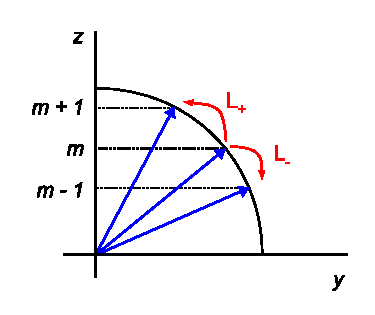
\includegraphics[scale=1]{zebrickoveoperatory.eps}
\caption[Posuvné operátory ve vektorovém modelu]{Činnost posuvných operátorů si můžeme představit tak, že operátor $\hat{L}_{+}$ mění kvantový stav $Y_l^m$ na kvantový stav $Y_l^{m+1}$ a operátor $\hat{L}_{-}$ mění kvantový stav $Y_l^m$ na stav $Y_l^{m-1}$.}
\label{obr:ZebrickoveOperatory}
\end{figure}

\subsection{Operátor momentu hybnosti v~polárních souřadnicích}
\label{kap:PolarniSouradnice}

Při popisu daného systému volíme takový souřadný systém, aby byl popis co možná nejjednodušší. V~případě přímočarého pohybu je nejvýhodnější souřadný systém pravoúhlých kartézských souřadnic $(x,y,z)$. Tento systém už ale není vhodný pro popis rotačních pohybů, protože popis křivosti je v~něm komplikovaný. Proto byly zavedeny křivočaré systémy souřadnic, které jednoduše popisují rotační pohyby.

Základní soustavou křivočarých souřadnic v~3D prostoru je sférická soustava $(r,\theta,\phi)$, kde $r$ je vzdálenost bodu od zvoleného počátku, $\theta$ je úhel, který svírá průvodič uvažovaného bod s~osou $z$ a $\phi$ je úhel, který svírá průvodič s~osou $x$. Abychom mohli přejít od kartézského souřadného systému do sférické souřadné soustavy, musíme odvodit transformační rovnice, které jednoznačně určují transformaci souřadnic $(x,y,z) \rightarrow (r,\theta,\phi)$. Z~geometrických úvah odvodíme transformační rovnice
\begin{equation}
x= r \sin \theta \cos \phi \mbox{,}
\label{rov:Hybnost39}
\end{equation}
\begin{equation}
y= r \sin \theta \sin \phi
\label{rov:Hybnost40}
\end{equation}
a
\begin{equation}
z = r \cos \theta \mbox{.}
\label{rov:Hybnost41}
\end{equation}
Obdobně odvodíme transformační rovnice pro inverzní transformaci $(r,\theta,\phi) \rightarrow (x,y,z)$
\begin{equation}
r^2=x^2+y^2+z^2 \mbox{,}
\label{rov:Hybnost42}
\end{equation}
\begin{equation}
\cos \theta = z/r
\label{rov:Hybnost43}
\end{equation}
a
\begin{equation}
\tan \phi = y/x \mbox{.}
\label{rov:Hybnost44}
\end{equation}

Dále nás bude zajímat, jaký způsobem se změní operátory momentu hybnosti, když od kartézských souřadnic přejdeme k~souřadnicím sférickým. Protože ve výrazech (\ref{rov:Hybnost6}), (\ref{rov:Hybnost7}) a (\ref{rov:Hybnost8}) pro operátory složek momentu hybnosti vystupují parciální derivace, nejprve si tyto derivace vyjádříme
\begin{equation}
\frac{\partial r}{\partial x} = \sin \theta \cos \phi, \quad \frac{\partial r}{\partial y} = \sin \theta \sin \phi, \quad \frac{\partial r}{\partial z} = \cos \theta \mbox{,}
\label{rov:Hybnost45}
\end{equation}
\begin{equation}
\frac{\partial \theta}{\partial x} = \frac{\cos \theta \cos \phi}{r}, \quad \frac{\partial \theta}{\partial y} = \frac{\cos \theta \sin \phi}{r}, \quad \frac{\partial \theta}{\partial z} = -\frac{\sin \theta}{r}
\label{rov:Hybnost46}
\end{equation}
a
\begin{equation}
\frac{\partial \phi}{\partial x} = -\frac{\sin \phi}{r \sin \theta}, \quad \frac{\partial \phi}{\partial y} = \frac{\cos \phi}{r \sin \theta}, \quad \frac{\partial \phi}{\partial z} = 0 \mbox{.}
\label{rov:Hybnost47}
\end{equation}
Pomocí vztahů (\ref{rov:Hybnost45}), (\ref{rov:Hybnost46}) a (\ref{rov:Hybnost47}) a pravidlu o~derivaci složené funkce odvodíme výrazy pro operátory složek momentu hybnosti ve sférických souřadnicích
\begin{equation}
\hat{L_x}= i \hbar \left( \sin \phi \frac{\partial}{\partial \theta} + \cot \theta \cos \phi \frac{\partial}{\partial \phi} \right) \mbox{,}
\label{rov:Hybnost48}
\end{equation}
\begin{equation}
\hat{L_y}= i \hbar \left( -\cos \phi \frac{\partial}{\partial \theta} + \cot \theta \sin \phi \frac{\partial}{\partial \phi} \right)
\label{rov:Hybnost49}
\end{equation}
a
\begin{equation}
\hat{L_z}= -i \hbar \frac{\partial}{\partial \phi} \mbox{.}
\label{rov:Hybnost50}
\end{equation}
Z~rovnice (\ref{rov:Hybnost50}) vidíme, proč se konvenčně pracuje se $z$-ovou složkou momentu hybnosti, protože její vyjádření ve sférických souřadnicích je nejjednodušší.

Když máme vyjádřeny jednotlivé operátory složek momentu hybnosti ve sférických souřadnicích, není problém vyjádřit ve sférických souřadnicích i operátor kvadrátu momentu hybnosti
\begin{equation}
\hat{L^2} = - \hbar^2 \left[ \frac{1}{\sin \theta} \frac{\partial}{\partial \theta} \left(\sin \theta \frac{\partial}{\partial \theta} \right) + \frac{1}{\sin^2 \theta}\frac{\partial^2}{\partial \phi^2} \right] \mbox{.}
\label{rov:Hybnost51}
\end{equation}

\subsection{Pohyb částice po kouli}
\label{kap:PohybCasticePoKouli}

V~tento okamžik máme potřebný aparát k~tomu, abychom mohli vyřešit problém pohybu částice s~momentem hybnosti. Naším cílem bude nalézt vlastní funkce $\psi(r, \theta, \phi)$ operátorů $\hat{L^2}$ a~$\hat{L_z}$. Tento jednoduchý problém nám poslouží  v~kapitole \ref{kap:vodik}, kde budeme řešit vodíkový atom.

Zapišme si nejprve vlastní problémy operátorů $\hat{L^2}$ a~$\hat{L_z}$
\begin{equation}
\hat{L^2}\psi(r, \theta, \phi) = l(l+1) \hbar^2 \psi(r, \theta, \phi)
\label{rov:Hybnost52}
\end{equation}
a
\begin{equation}
\hat{L_z}\psi(r, \theta, \phi) = m \hbar \psi(r, \theta, \phi) \mbox{,}
\label{rov:Hybnost53}
\end{equation}
kde jsme za vlastní čísla dosadili ze vztahů \eqref{rov:VlastniCislaKvadratu} a \eqref{rov:VlastniCislaZSlozky}. Protože operátor $\hat{L}^2$ ani operátor $\hat{L}_z$ nepůsobí na souřadnici $r$, můžeme provést separaci proměnných
\begin{equation}
\psi(r, \theta, \phi) = R(r) Y (\theta, \phi),
\label{rov:Hybnost54}
\end{equation}
kde $R(r)$ je radiální část vlnové funkce a $Y(\theta,\phi)$ je angulární část vlnové funkce, kterou označujeme jako sférické harmoniky. Díky separaci proměnných se problém pohybu částice v~3D prostoru rozpadl na pohyb částice po kulové sféře, popsaný pomocí sférické harmoniky a na vyšetření pohybu částice po daném orbitu ve vzdálenosti $r$ od zvoleného počátku, který je popsaný radiální částí vlnové funkce. Separace proměnných (\ref{rov:Hybnost54}) umožňuje zvlášť vyšetřit pohyb po kulové sféře a zvlášť radiální pohyb. V~tuto chvíli nás zajímá pouze pohyb po kulové sféře, proto budeme dále pracovat jen s~vlnovou funkcí ve tvaru sférické harmoniky $Y(\theta, \phi)$.

Operátor $\hat{L_z}$ působí pouze na souřadnici $\phi$ (viz vztah (\ref{rov:Hybnost50})), proto můžeme předpokládat, že i sférické harmoniky můžeme separovat
\begin{equation}
Y(\theta, \phi) = \Theta (\theta) \Phi (\phi) \mbox{.}
\label{rov:Hybnost55}
\end{equation}

Vyřešme nejprve vlastní problém (\ref{rov:Hybnost53}), kde za operátor $\hat{L_z}$ dosadíme ze vztahu (\ref{rov:Hybnost50}) a~dále využijeme separaci proměnných (\ref{rov:Hybnost55})
\begin{equation}
-i \hbar \Theta \frac{\partial \Phi}{\partial \phi} = m \hbar \Theta \Phi \mbox{.}
\label{rov:Hybnost56}
\end{equation}
Rovnici dále upravme
\begin{equation}
-i  \frac{\mathrm{d} \Phi}{\Phi} = m \mathrm{d} \phi
\label{rov:Hybnost57}
\end{equation}
a dostaneme obyčejnou diferenciální rovnici pro $\Phi(\phi)$. Integrací rovnice (\ref{rov:Hybnost57}) získáme řešení ve tvaru
\begin{equation}
\Phi = A e^{i m \phi} \mbox{,}
\label{rov:Hybnost58}
\end{equation}
kde $A$ je integrační konstanta. Tu určíme z~normovací podmínky
\begin{equation}
\int_{0}^{2\pi} \Phi^{\ast}\Phi \mathrm{d} \phi \stackrel{a}{=} A^2 \int_{0}^{2\pi} \mathrm{d} \phi = 2 A^2 \pi = 1 \Rightarrow A = \frac{1}{\sqrt{2 \pi}} \mbox{.}
\label{rov:Hybnost59}
\end{equation}
Úprava $a$ plyne z~následujícího
\begin{equation}
\Phi^{\ast}\Phi = e^{-i m \phi}e^{i m \phi}=e^0=1 \mbox{.}
\label{rov:Hybnost60}
\end{equation}
Integrační meze ve vztahu (\ref{rov:Hybnost59}) plynou z~toho, že ve sférických souřadnicích platí $\phi \in \langle 0;2\pi\rangle$. Sférickou harmoniku $Y(\theta, \phi)$ tak můžeme zapsat jako
\begin{equation}
Y(\theta, \phi) = \Theta(\theta) \Phi(\phi) = \Theta(\theta) \frac{1}{2\pi}e^{im\phi} \mbox{.}
\label{rov:Hybnost61}
\end{equation}

Dosazením sférické harmoniky (\ref{rov:Hybnost61}) do vlastního problému (\ref{rov:Hybnost52}) operátoru $\hat{L^2}$ a řešením vzniknuvší diferenciální rovnice bychom došli k~závěru, že se jedná o~typ diferenciální rovnice, která se řeší pomocí ortogonálních polynomů, konkrétně pomocí přidružených Lagendrových polynomů $S_l^{|m|}(\cos \theta)$. Pak se ukáže, že platí
\begin{equation}
\Theta(\cos \theta) \equiv S_l^{|m|} (\cos \theta) \mbox{.}
\label{rov:Hybnost62}
\end{equation}
Výslednou sférickou harmoniku $Y_l^{m}$ tak můžeme zapsat ve tvaru
\begin{equation}
\boxed{Y_l^{m}(\theta, \phi) = N_{lm} S_l^{|m|} (\cos \theta) e^{i m \phi} \mbox{,}}
\label{rov:Hybnost63}
\end{equation}
kde $N_{lm}$ je normovací faktor
\begin{equation}
N_{lm} = \sqrt{\frac{(l-|m|)! (2l+1)}{4\pi(l+|m|)!}}\mbox{.}
\label{rov:Hybnost64}
\end{equation}

Závěr našeho snažení je následující. Pohyb částice po kulové sféře můžeme popsat pomocí sférických harmonik, neboli angulární část vlnové funkce $\psi(r,\theta,\phi)$. Sférické harmoniky $Y_l^{m}(\theta, \phi)$ závisí pouze na úhlech $\theta$ a $\phi$ a jsou parametrizovány dvojicí kvantových číslech $l$ a $m$. Obecně se jedná o~komplexní funkce, na jejichž zobrazení bychom potřebovali 6-ti dimenzionální prostor (jedná se o~3D funkce v~komplexní rovině). Proto nezobrazujeme přímo sférické harmoniky, ale jejich lineární kombinace.

\subsection{Energie pohybu po sféře}
\label{kap:EnergiePohybSfera}

Budeme-li chtít určit energii částice, která se pohybuje po kulové sféře, zapíšeme vlastní problém pro energii, tj. Schrödingerovu rovnici s~hamiltoniánem ve tvaru
\begin{equation}
\hat{H} = -\frac{\hbar^2}{2m}\nabla^2 \mbox{,}
\label{rov:Hybnost65}
\end{equation}
kde předpokládáme, že částice se nepohybuje v~žádném potenciálu, tj. $V=0$. Protože hamiltonián $\hat{H}$ komutuje s~operátory $\hat{L^2}$ a $\hat{L_z}$, mají tyto operátory společný soubor vlastních funkcí, kterými jsou sférické harmoniky $Y_l^m$.

Budeme postupovat tak, že si operátor $\nabla^2$ vyjádříme ve sférických souřadnicích
\begin{equation}
\nabla^2 = \frac{\partial^2}{\partial r^2} + \frac{2}{r}\frac{\partial}{\partial r} + \frac{1}{r^2}\Lambda^2 \mbox{,}
\label{rov:Hybnost66}
\end{equation}
kde operátor $\Lambda^2$ je legendrián, který představuje angulární část operátoru $\nabla^2$
\begin{equation}
\Lambda^2 = \frac{1}{\sin^2 \theta}\frac{\partial^2}{\partial \phi^2} + \frac{1}{\sin \theta}\frac{\partial}{\partial \theta}\sin \theta \frac{\partial}{\partial \theta}\mbox{.}
\label{rov:Hybnost67}
\end{equation}
Protože nás zajímá pouze pohyb po kulové sféře, kde se nemění souřadnice $r$ zredukuje se operátor $\nabla^2$ na $\Lambda^2$. Uvědomíme-li si, že moment setrvačnosti je definován jako $I=mr^2$, můžeme Schrödingerovu rovnici pro pohyb na kulové ploše zapsat jako
\begin{equation}
\Lambda^2 Y_l^m = - \frac{2 I E}{\hbar^2} Y_l^m \mbox{.}
\label{rov:Hybnost68}
\end{equation}
Dále je možné ukázat, že platí 
\begin{equation}
\Lambda^2 Y_l^m = -l(l+1) Y_l^m \mbox{.}
\label{rov:Hybnost69}
\end{equation}
Porovnáním rovnic (\ref{rov:Hybnost68}) a (\ref{rov:Hybnost69}) dostaneme pro energii
\begin{equation}
\boxed{E_{lm} = l(l+1)\frac{\hbar^2}{2I} \mbox{,}}
\label{rov:Hybnost70}
\end{equation}
kde každý energetický stav $E_{lm}$ je $2l+1$ degenerovaný.

\begin{priklad}
\textbf{Zadání}: Délky vazeb jsou určovány ze spektroskopických měření, která jsou velice přesná. Z rotačního spektra HCl jsme odvodili, že $B=10{,}59342$~cm$^{-1}$. Hmotnosti $^1$H a $^{35}$Cl jsou $1{,}0078250$ a $34{,}9688527$~a.u. Odvoďte délku vazby v molekule HCl.\\[0.1cm]
\textbf{Řešení:} Pro rotační konstantu $B$ platí
\begin{displaymath}
B = \frac{h}{8 \pi^2 \mu c r_0^2},
\end{displaymath} 
kde $\mu$ je redukovaná hmotnost. Pak
\begin{displaymath}
r_0 = \sqrt{\frac{h}{8 \pi^2 \mu c B}} = 1{,}274553 \cdot 10^{-10} \mbox{ m}.
\end{displaymath} \vspace{-0.7cm}
\end{priklad}

\clearpage
\section{Elektronový spin}
\label{kap:elektronovyspin}
Elektronový spin je veličina poněkud záhadná. Je to veličina, která nemá obdoby v~klasickém světě. Do kvantové mechaniky se spin dostal jako experimentální fakt: z~řady experimentů totiž vyplývalo, že kromě orbitálního momentu má elektron ještě nějaký dodatečný moment hybnosti. V~nerelativistické kvantové teorii jeho existenci prostě postulujeme. Elektronový spin ovšem přirozeným způsobem vyplynul ze snahy vytvořit relativistickou kvantovou teorii, viz kapitola~\ref{kap:relativita}. Toto téma jde však za rámec našeho stručného textu.

\subsection{Pojem spinu}
\label{kap:PojemSpinu}

Spin je vlastní moment hybnosti částice, kupříkladu elektronu. V~následujících oddílech se stručně seznámíme s~tím, jak se vlastně na existenci spinu přišlo.

V~kapitole~\ref{kap:momenthybnosti} jsme se blíže seznámili s~orbitálním momentem, který je v~klasické fyzice definován vztahem
\begin{equation}
\mathbf{L} \equiv \mathbf{r} \times \mathbf{p} \mbox{,}
\label{rov:Spin1}
\end{equation}
kde $\mathbf{r}$ je kolmá vzdálenost od osy otáčení a $\mathbf{p} = m \mathbf{v}$ je hybnost. Moment hybnosti $\mathbf{L}$ označujeme jako orbitální z~toho důvodu, že objekt, který obíhá okolo daného středu po tzv. orbitu, má nenulový orbitální moment. V~případě atomu si můžeme představit elektron, který obíhá kolem atomového jádra. Protože elektron nese elementární náboj $e$, generuje při svém orbitálním pohybu proudovou smyčku, která vytváří magnetické pole. Sílu takto vzniklého pole měříme pomocí magnetického momentu spojeného s~orbitálním momentem hybnosti
\begin{equation}
\mu_L = -\frac{e}{2m_e}\mathbf{L} \mbox{.}
\label{rov:Spin2}
\end{equation}
Vztah (\ref{rov:Spin2}) je uveden pro případ elektronu -- hmotnost $m_e$ a náboj $e$. Obecně by ve vztahu figurovala hmotnost částice $m$ a náboj částice $q$. 

Uvažujme nyní atom, ve kterém rotuje elektron. Takovýto atom může mít nenulový magnetický moment, který jsme schopni změřit například pomocí vychylování směru atomu v~nehomogenním magnetickém poli. Potenciální energie interakce magnetického momentu s~vnějším magnetickým polem je
\begin{equation}
U_{int} = - \vec{\mu} \cdot \vec{B} = - \vert \vec{\mu} \vert B \cos \theta,
\nonumber
\end{equation}
kde $\vec{\mu}$ je magnetický moment, $B$ je magnetická indukce vnějšího pole a $\theta$ je úhel, který svírají tyto vektory. Bez újmy na obecnosti zvolme směr magnetického pole ve směru osy $z$, pak dostaneme
\begin{equation}
U_{int} = - \mu_z B = \left( \frac{e \hbar}{2 m_e} \right) m B
\label{rov:Spin26}
\end{equation}

\noindent Výraz v~závorce ve vztahu \eqref{rov:Spin26} se označuje jako Bohrův magneton a má hodnotu $\mu_B = 9,27 \cdot 10^{-24} \joule \tesla^{-1}$. Vidíme, že ve vnějším magnetickém poli závisí energie elektronu na magnetickém kvantovém čísle $m$.

Tak například elektronový stav s~vedlejším kvantovým číslem $l = 1$ (p-orbital) by se měl ve vnějším magnetickém poli rozštěpit do tří různých stavů s~různou energií podle hodnot magnetického kvantového čísla $m = -1, 0, 1$. To vede k~rozštěpení původní jediné spektrální čáry v~atomovém spektru do tripletu, přičemž vzdálenost mezi čárami závisí na velikosti magnetického pole, tj. magnetické indukci $\mathbf{B}$ (viz obrázek~\ref{obr:Zeeman}). Štěpení spektrálních čar v~magnetickém poli se nazývá Zeemanův jev po svém objeviteli holandském fyzikovi Zeemanovi, který ho poprvé pozoroval v~roce 1896. Zeemanův jev je tak přímým experimentálním potvrzením prostorového kvantování momentu hybnosti.\footnote{Ve skutečnosti je štěpení čar v magnetickém poli komplikovanější díky spinu.}

\begin{figure} [htb]
\centering
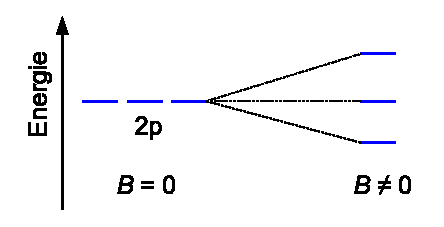
\includegraphics[scale=1]{Zeeman.eps}
\caption{Štěpení čar v magnetickém poli.}
\label{obr:Zeeman}
\end{figure}

Ve skutečnosti se ukázalo, že štěpení atomových hladin v~magnetickém poli může být o~dost složitější, než předpovídala kvantová mechanika. Toto  anomální chování (anomální Zeemanův jev) bylo možno vysvětlit zavedením dodatečného momentu hybnosti elektronu, tedy spinu. Nejjasnější experimentální důkaz existence spinu podal experiment provedený v~roce 1922 Otto Sternem a Walterem Gerlachem. Tento experiment si proto probereme důkladněji.    


\subsection{Sternův-Gerlachův experiment}
\label{kap:SG experiment}

Experimentální aparatura (viz obrázek~\ref{obr:SCH-experiment}) Sternova-Gerlachova experimentu sestávala z~pícky, ve které se zahřívaly atomy stříbra. Páry stříbra opouštěly pícku malým otvorem a~vytvářely paprsek atomů. Paprsek procházel nehomogenním magnetickým polem a dopadal na vhodné stínítko, které sloužilo k~vizualizaci výsledků. Předpokladem experimentu je, že atomy stříbra mají nenulový magnetický moment. Atomy s~nenulovým magnetickým momentem interagují s~nehomogenním magnetickým polem a jsou vychýleny z~přímého směru v~závislosti na prostorové orientaci magnetického momentu. Zvolme orientaci nehomogenního magnetického pole ve směru osy $z$. Pak pro sílu, která způsobuje vychýlení atomů z~přímé dráhy platí
\begin{equation}
F_z = - \frac{\partial U}{\partial z } \mbox{,}
\label{rov:Spin5}
\end{equation}
kde $U = - \mu \cdot B = - \mu_z B_z$ je potenciální energie atomů stříbra v~magnetickém poli orientovaném ve směru $z$-ové osy. Proto 
\begin{equation}
F_z = \mu_z \frac{\partial B}{\partial z } \mbox{.}
\label{rov:Spin6}
\end{equation}

\begin{figure} [!ht]
\centering
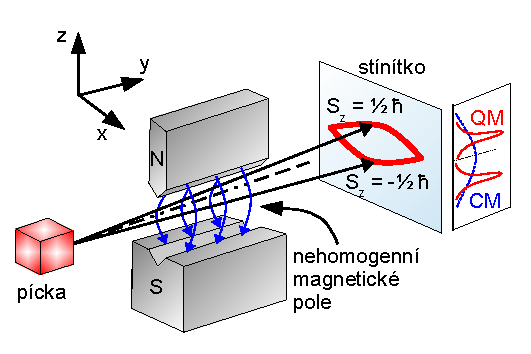
\includegraphics[scale=1]{SGE.pdf}
\caption[Sternův-Gerlachův experiment]{Schématické zobrazení experimentální aparatury, kterou použili Stern s~Gerlachem při experimentu, kterým chtěli prokázat prostorové kvantování orbitálního momentu hybnosti. Ve skutečnosti prokázali existenci spinu, dalšího momentu hybnosti elektronu. Aparatura se skládala z~pícky s~atomy stříbra, které ze zahřály a opouštěly pícku malým otvorem, přičemž tvořily atomový paprsek. Atomy procházely nehomogenním magnetickým polem a~vychylovaly se v~závislosti na prostorové orientaci spinu. Po dopadu na stínítko se vytvořily dvě stopy odpovídající dvěma prostorovým projekcím spinu -- spin nahoru a spin dolů. Dále je zobrazeno porovnání očekávané distribuce dopadů atomů stříbra na stínítko podle klasické (CM) a~kvantové (QM) mechaniky.}
\label{obr:SCH-experiment}
\end{figure}


Podle představ klasické fyziky bude magnetický moment stříbrných atomů orientován v~prostoru zcela náhodně a jeho průmět do osy z~tak bude také nabývat libovolných hodnot od -$|\mu|$ do $|\mu|$. Na stínítku bychom dostali přímou čáru o~velikosti ve směru $z$-ové osy odpovídající dopadům stříbrných atomů. Stříbrné atomy ale dopadaly na stínítko pouze ve dvou bodech, které odpovídaly dipólovému momentu
\begin{equation}
\mu_z = \pm \mu_B, \quad \mu_B = \frac{e\hbar}{2m_e}\mbox{,}
\label{rov:Spin7}
\end{equation}
kde $\mu_B$ je Bohrův magneton. Stern s~Gerlachem byli nadšeni, neboť tento experiment potvrzoval kvantování momentu hybnosti ve směru osy z, jak předpovídala kvantová teorie. Jenže pozornější pohled už ukazuje, že zde něco nesouhlasí.  Atomy stříbra mají 47 elektronů, z~nichž 46 je spárovaných, a tudíž nepřispívají k~orbitálnímu momentu hybnosti. Zbývající 1 nespárovaný elektron má také nulový orbitální mement hybnosti, protože obsazuje $5s$ orbital. Celkový orbitální moment hybnosti atomů stříbra je tedy $\mathbf{L}=0$, a tak neexistuje žádný magnetický moment vyvolaný tímto momentem hybnosti. Můžeme připustit, že onen nespárovaný elektron se z~nějakých důvodu bude nacházet v~p orbitalu. V~této situaci by se ale měl svazek stříbra rozpadat na tři, nikoliv na dva podsvazky. Pozorovaný nenulový magnetický moment atomů stříbra musí být vyvolán dalším momentem hybnosti -- spinem. Sternův - Gerlachův experiment tak představuje přímou experimentální metodu umožňující měřit jednu z~komponent spinu, v~našem případě $z$-ovou komponentu. Koncept spinu elektronu byl zaveden až v~roce 1925 holandskými fyziky Georgem Uhlenbeckem a Samuelem Goudsmitem, kteří analyzovali atomová spektra. I~přesto je Sternův - Gerlachův experiment považován za experimentální důkaz existence elektronového spinu.


\subsection{Spin a rotace elektronu kolem své osy}

Samotné slovo \uv{spin} je odvozeno z~anglického slovesa \uv{\textit{to spin}}, tedy točiti se, vířiti, vrtěti se. Odkazuje na představu, že spin je moment hybnosti spojený s~vlastní rotací částice. Takový výklad je ovšem pochybený. Budeme-li si představovat spin jako moment hybnosti spojený s~rotujícím objektem (například pohyb planety Země otáčející se kolem své osy je spojen s~momentem hybnosti, můžeme příslušný moment hybnosti určit pomocí vztahu
\begin{equation}
\mathbf{S} = I \omega \mbox{,}
\label{rov:Spin3}
\end{equation}
kde moment hybnosti  $S$ nazveme spinovým momentem hybnosti či krátce spinem,  $I$ je moment setrvačnosti související s~distribucí hmoty objektu okolo osy rotace a $\omega$ je úhlová rychlost. Spin je vektorová veličina orientovaná v~ose rotace a jeho směr je určen pomocí pravidla pravé ruky. Pakliže je rotující objekt nabitý, jeho rotace opět způsobí vznik magnetického pole. I~zde charakterizujeme magnetické pole magnetickým momentem, tentokráte spojeným se spinovým momentem hybnosti
\begin{equation}
\mu_S = \frac{q}{2m}\mathbf{S} \mbox{,}
\label{rov:Spin4}
\end{equation}
kde $q$ je náboj rotujícího tělesa.

Elementární částice jako je elektron jsou bodové částice a nedá se tak mluvit o~jejich rotaci. To znamená, že moment setrvačnosti jde k~nule, $I \rightarrow 0$, a proto i spin částic se bude blížit nule, $\mathbf{S} \rightarrow 0$. Kdyby tomu tak bylo, elementární částice by neměly žádný dipólový moment související se spinem, což je v~rozporu s~experimentem. Ve snaze zlepšit tuto neshodu můžeme připustit, že elementární částice jsou velmi malé rotující kuličky. Z~experimentů plyne, že poloměry částic jsou $< 10^{-17} \,\mbox{m}$. Aby například elektron s~tímto poloměrem měl příslušnou hodnotu svého spinu, musel by rotovat daleko větší rychlostí, než je rychlost světla. Tento rozpor vede k~tomu, že klasická mechanika při popisu elementárních částic selhává a musíme jí nahradit kvantovou teorií.


\subsection{Spin v~kvantové mechanice}
\label{kap:Spin-QM}

Pojďme nyní zavést spin do formalismu kvantové mechaniky. Ze Sternova-Gerlachova experimentu jsme nahlédli, že spin má vlastnosti momentu hybnosti. Pro spin by tak měly platit ty samé vztahy jako pro moment hybnosti. V~kapitole (\ref{kap:momenthybnosti}) jsme dospěli k~závěru, že velikost orbitálního momentu hybnosti $\mathbf{L}$ je kvantována 
\begin{equation}
L = \sqrt{l(l+1)}\hbar, \quad l=0,1,2,\dots \mbox{,}
\label{rov:Spin8}
\end{equation}
kde $l$ je vedlejší kvantové číslo. A~dále, že jedna ze~složek orbitálního momentu hybnosti, řekněme $L_z$, je také kvantována
\begin{equation}
L_z = m_l \hbar, \quad m_l=-l,\dots, 0, \dots, +l \mbox{,}
\label{rov:Spin9}
\end{equation}
kde $m_l$ je magnetické kvantové číslo. Kvantování složky orbitálního momentu hybnosti je vyjádřením prostorového kvantování, tj. že vektor orbitálního momentu hybnosti může mít jen určité prostorové orientace.

Je logické předpokládat, že pro spin budou platit obdobné relace, jako pro orbitální moment hybnosti. Proto velikost spinového momentu hybnosti $\mathbf{S}$ je kvantována jako
\begin{equation}
\boxed{S = \sqrt{s(s+1)}\hbar, \quad s=0,1/2,1,3/2 \dots \mbox{,}}
\label{rov:Spin10}
\end{equation}
kde $s$ je spinové kvantové číslo, které v~případě elektronu má hodnotu $s=1/2$, a tak velikost spinu elektronu je $S = \sqrt{3/4}\hbar$. Podobně i jedna z~komponent spinu, konvenčně $S_z$, je kvantována
\begin{equation}
\boxed{S_z = m_s \hbar, \quad m_s= -s, \dots, 0, \dots, +s \mbox{,}}
\label{rov:Spin11}
\end{equation}
kde $m_s$ je magnetické spinové kvantové číslo, které v~případě elektronu nabývá hodnot $m_s=\pm 1/2$. Elektron se tak může nacházet ve dvou stavech lišících se průmětem momentu hybnosti do osy z, plně v~souladu se Sternovým-Gerlachovým experimentem. Vidíme, že vztahy (\ref{rov:Spin10}) a (\ref{rov:Spin11}) pro spin jsou obdobou vztahů (\ref{rov:Spin8}) a (\ref{rov:Spin9}) pro orbitální moment hybnosti s~tím rozdílem, že v~případě spinu nabývá spinové kvantové číslo $s$ poločíselných hodnot. 

V~úvodu jsme poznali, že moment hybnosti je příčinou nenulového magnetického momentu (viz vztahy (\ref{rov:Spin2}) a (\ref{rov:Spin4})). Mezi spinovým momentem a magnetickým momentem platí vztah
\begin{equation}
\boxed{\mu_S = g_e \frac{e}{2m_e}\mathbf{S} \mbox{,}}
\label{rov:Spin12}
\end{equation}
kde $g_e$ je tzv. gyromagnetický poměr, který pro elektron má hodnotu $g_e\doteq2$. Gyromagnetický poměr je v~nerelativistické kvantové mechanice veličinou, která musí být změřena, v~rámci relativistické kvantové teorie elektronu je ovšem možné jej vypočítat. Gyromagnetický poměr vyjadřuje podíl magnetického dipólového momentu a orbitálního momentu hybnosti.

Z~experimentu vyplývá toliko hodnota velikosti momentu hybnosti a průmětu momentu hybnosti do osy z. Abychom teorii učinili úplnou, můžeme formálně zapsat operátorové rovnice pro operátory spinového momentu $\hat{S^2}$ a $\hat{S_z}$. Jednotlivé rovnice jsou
\begin{equation}
\boxed{\hat{S^2}\alpha = \hbar^2 s(s+1)\alpha \mbox{,}}
\label{rov:Spin17}
\end{equation}
\begin{equation}
\boxed{\hat{S^2}\beta = \hbar^2 s(s+1)\beta \mbox{,}}
\label{rov:Spin18}
\end{equation}
\begin{equation}
\boxed{\hat{S_z}\alpha= \frac{1}{2}\hbar \alpha \mbox{,}}
\label{rov:Spin19}
\end{equation}
\begin{equation}
\boxed{\hat{S_z}\beta= -\frac{1}{2}\hbar \beta \mbox{.}}
\label{rov:Spin20}
\end{equation}

\noindent kde $\alpha$ a $\beta$ jsou tzv. spinové vlnová funkce. Vlnová funkce $\alpha$ nám neříká nic jiného, než je elektron má spin mířící \uv{nahoru}, tedy s~$m_s=1/2$, vlnová funkce $\beta$ má zase spin orientovaný \uv{dolů}, tedy je charakterizována spinovým magnetickým číslem  $m_s=1/2$. Formálně tuto skutečnost zapíšeme následujícími rovnicemi: 

\begin{equation}
\alpha(m_s=1/2)=1, \quad \alpha(m_s=-1/2)=0
\label{rov:Spin13}
\end{equation}
a
\begin{equation}
\beta(m_s=1/2)=0,  \quad \beta(m_s=-1/2)=1 \mbox{.}
\label{rov:Spin14}
\end{equation}
Spinové funkce tak nejsou funkcemi prostorových souřadnic, nýbrž magnetických kvantových čísel. Takto zavedené spinové vlnové funkce jsou normalizované. Například pro $\alpha$ platí
\begin{equation}
\int |\alpha|^2 \mathrm{d}\tau \Rightarrow \sum_{-1/2}^{1/2}|\alpha|^2 = \alpha(1/2) \alpha(1/2) + \alpha(-1/2)\alpha(-1/2) = 1 + 0 = 1 \mbox{.}
\label{rov:Spin15}
\end{equation}
V~rovnici (\ref{rov:Spin15}) značí $\mathrm{d}\tau$ integraci přes celý prostor. Protože spinové funkce jsou definovány na diskrétních hodnotách spinových magnetických čísel, přejde integrace na sumaci. Suma vyjde jednotková. Stejný závěr bychom dostali v~případě spinové vlnové funkce $\beta$. Spinové vlnové funkce jsou i ortogonální. Důkaz provedeme následovně
\begin{equation}
\sum_{-1/2}^{1/2} \alpha(m_s) \beta(m_s) = \alpha(1/2) \beta(1/2) + \alpha(-1/2) \beta(-1/2) = 0 + 0 = 0 \mbox{,}
\label{rov:Spin16}
\end{equation}
kde máme na paměti, že nutná podmínka ortogonality vlnových funkcí je, že integrál, v~tomto případě suma, přes celý prostor je rovna nule.

Na první pohled může zavedení spinových operátorů a spinových funkcí působit samoúčelně. Ukáže se však, že pro zápis vlnové funkce atomů s~více elektrony tyto funkce budeme potřebovat.



\subsection{Spin v~magnetickém poli}
\label{kap:SpinMagPole}

V~případě Sternova - Gerlachova experimentu jsme se setkali s~tím, že spin elektronu interaguje s~vnějším magnetickým polem. Pro potenciální energii této interakce je možné psát
\begin{equation}
U_{int} = - \mu_S \cdot \mathbf{B} \mbox{,}
\label{rov:Spin21}
\end{equation}
kde $\mathbf{B}$ je magnetická indukce vnějšího magnetického pole. Orientujeme-li pole ve směru osy $z$, tj. $\mathbf{B}=(0, 0, B_z)$, a za dipólový moment dosadíme ze vztahu (\ref{rov:Spin12}) dostaneme pro potenciální energii interakce
\begin{equation}
U_{int} = -\mu_z B_z = -g_e \frac{e}{2m_e} B_z S_z = -g_e \frac{e}{2m_e} B_z  m_s \hbar  = \gamma B_z \hbar m_s \mbox{.}
\label{rov:Spin22}
\end{equation}
Za $z$-ovou komponentu spinu jsme dosadili její vlastní hodnotu $S_z = m_s \hbar$ a dále konstanty $(g_e e)/(2m_e)$ jsme zahrnuli do jednoho faktoru $\gamma$, který se nazývá g-faktor. Protože kvantové číslo $m_s$ v~případě elektronu může nabývat dvou hodnot $\pm 1/2$, dojde ve vnějším magnetickém poli k~různě silné interakci elektronů v~závislosti na prostorové orientaci jejich spinů. Rozdíl energií daný různou orientací spinu je roven
\begin{equation}
\Delta U_{int} = \gamma B_z \hbar \mbox{.}
\label{rov:Spin23}
\end{equation}
Rovnice (\ref{rov:Spin23}) je základem experimentálních technik EPR (elektronová paramagnetická rezonance) a NMR (nukleární magnetická rezonance) spektroskopie. V~případě NMR je nutné uvažovat g-faktor pro sledované jádro
\begin{equation}
\gamma_N = g_N \frac{e}{2m_N} \mbox{,}
\label{rov:Spin24}
\end{equation}
kde $m_N$ a $g_N$ jsou po řadě hmotnost daného jádra a jeho gyromagnetický poměr.

\begin{priklad}
\textbf{Zadání:} Spočítejte dvě možné energie nukleárního spinu pro jádro $^1$H v magnetickém poli 5,50~T.\\[0.1cm]
\textbf{Řešení:} Energie jsou dány vztahem
\begin{displaymath}
U_{int} = \gamma_N \hbar m_s B_z = \pm 7{,}76 \cdot 10^{-26} \mbox{ J}.
\end{displaymath}

\textbf{Zadání:} Spočítejte energetický rozdíl těchto dvou stavů. Jakou vlnovou délku by muselo být elektromagnetické záření, aby došlo k absorpci z jednoho stavu do druhého? \\[0.1cm]
\textbf{Řešení:} Energetický rozdíl bude
\begin{displaymath}
\Delta E = 2 \cdot U_{int} = 1{,}55 \cdot 10^{-25} \mbox{ J}.
\end{displaymath}
Vlnová délka fotonu pak je
\begin{displaymath}
\lambda = \frac{c}{\nu} = \frac{c}{\frac{\Delta E}{h}} = 1{,}282 \mbox{ m}.
\end{displaymath} \vspace{-0.5cm}
\end{priklad}


\clearpage
\section{Problém dvou částic}
\label{kap:dvecastice}
Do této chvíle jsme se zabývali pouze pohybem jedné částice v~jednom rozměru. Tušíme přitom, že popis pohybu dvou a více částic (ve dvou a více rozměrech) bude o~něco složitější. Pokud nás ale zajímají jen dvě částice, zůstane vše poměrně jednoduché. Řešení problému dvou částic je přitom v~chemii velmi důležité. Budeme ho potřebovat při hledání energetických stavů rotující či vibrující molekuly nebo při popisu atomů vodíkového typu.

\subsection{Pohyb nezávislých částic: metoda separace proměnných}

 Uvažujme pohyb dvou částic podél osy \textit{x}, přičemž předpokládáme, že částice na sebe vzájemně nepůsobí. Hamiltonián pak můžeme zapsat jako součet Hamiltoniánů popisujících na jednotlivé částice:

\begin{equation}
\hat{H}=\hat{H_{1}}+\hat{H_{2}},
\label{rov:2č-nez1}
\end{equation}

\noindent kde $\hat{H_{1}}$ závisí toliko na souřadnici první částice $x_{1}$ a $\hat{H_{2}}$ pouze na souřadnici druhé částice $x_{2}$. Schr\"odingerova rovnice pak bude vypadat následovně:

\begin{equation}
(\hat{H_{1}}+\hat{H_{2}})\psi(x_{1},x_{2})=E\psi(x_{1},x_{2})
\label{rov:2č-nez2}
\end{equation}

Vlnovou funkci pro dvě částice budeme hledat ve tvaru součinu vlnových funkcí popisujících nezávislé částice:

\begin{equation}
\psi(x_{1},x_{2})=\psi_{1}(x_{1})\psi_{2}(x_{2})
\label{rov:2č-nez3}
\end{equation}

Takovémuto zápisu říkáme separace proměnných. Nejspíše je zřejmé, proč hledáme řešení v~tomto tvaru. Vlnová funkce je spojena s~pravděpodobností výskytu elektronu. Čtverec vlnové funkce na levé straně rovnice \ref{rov:2č-nez3} nám tak udává pravděpodobnost, že se částice 1 nachází v~poloze $x_{1}$ a zároveň se částice 2 nachází v~poloze $x_{2}$. Pravou stranou rovnice \ref{rov:2č-nez3} pak tvrdíme, že tato pravděpodobnost je rovna pravděpodobnosti, že se částice 1 nachází v~poloze  $x_{1}$ nezávisle na poloze částice 2, násobena pravděpodobností nalezení částice 2 v~bodě $x_{2}$ bez ohledu na polohu částice 1. Jinými slovy předpokládáme, že oba jevy jsou nezávislé. To je předpoklad rozumný, neboť obě částice na sobě silově nepůsobí. Znovu zdůrazněme, že vlnová funkce $\psi_{1}$ závisí pouze na souřadnicích částice 1 a vlnová funkce $\psi_{1}$ na souřadnicích částice 2. Nyní přepišme Schr\"odingerovu rovnici pomocí vlnové funkce v~separovaném tvaru:

\begin{equation}
\hat{H_{1}}\psi_{1}(x_{1})\psi_{2}(x_{2})+\hat{H_{2}}\psi_{1}(x_{1})\psi_{2}(x_{2})=E\psi_{1}(x_{1})\psi_{2}(x_{2})
\label{rov:2č-nez44}
\end{equation}


Hamiltonián první částice působí pouze na první částici. Vlnovou funkci druhé částice tedy můžeme brát jako konstantu. Po vydělení $\psi_{1}\psi_{2}$ upravíme Schr\"odingerovu rovnici na následující tvar: 

\begin{equation}
\frac{\hat{H_{1}}\psi_{1}(x_{1})}{\psi_{1}(x_{1})}+\frac{\hat{H_{2}}\psi_{2}(x_{2})}{\psi_{2}(x_{2})}=E
\label{rov:2č-nez5}
\end{equation}

První ze sčítanců na levé straně rovnice \ref{rov:2č-nez5} je funkcí pouze souřadnice $x_{1}$, druhý pak pouze souřadnice $x_{2}$. Součet obou členů musí být přitom konstantní pro každou kombinaci  $x_{1}$ a $x_{2}$. To obecně není možno splnit jinak než, že oba dva sčítance jsou rovny konstantám, které si označíme jako $E_{1}$ a $E_{1}$:

\begin{equation}
\hat{H_{1}}\psi_{1}(x_{1})=E_{1}\psi_{1}(x_{1})
\label{rov:2č-nez6}
\end{equation}
\begin{equation}
\hat{H_{2}}\psi_{2}(x_{2})=E_{2}\psi_{2}(x_{2})
\label{rov:2č-nez7}
\end{equation}
\begin{equation}
E=E_{1}+E_{2}
\label{rov:2č-nez8}
\end{equation}

Schr\"odingerova rovnice pro dvě proměnné se nám tak rozpadla na dvě Schr\"odingerovy rovnice o~jedné proměnné. Místo jedné složité úlohy tak vyřešíme dvě úlohy jednoduché. Energie pohybu obou částic dohromady je dána součtem energií jednotlivých částic a vlnová funkce pro dvě částice je dána součinem dvou jednočásticových vlnových funkcí. Naše úvahy můžeme snadno rozšířit na situaci, kdy se
\begin{itemize}
\item jedna jedna částice pohybuje ve dvou rozměrech: 

\begin{equation}
\psi(x,y)=\psi_{1}(x)\psi_{2}(y)
\label{rov:2č-nez9}
\end{equation}

\item dvě částice pohybují ve třech rozměrech:

\begin{equation}
\psi(x_{1},y_{1},z_{1},x_{2},y_{2},z_{2})=\psi_{1}(x_{1},y_{1},z_{1})\psi_{2}(x_{2},y_{2},z_{2})
\label{rov:2č-nez4}
\end{equation}

\item N částic pohybuje ve třech rozměrech:
\begin{equation}
\psi(x_{1},y_{1},z_{1},...,x_{i},y_{i},z_{i},...,x_{N},y_{N},z_{N})=
\prod_{i=1}^N\psi_{i}(x_{i},y_{i},z_{i})
\label{rov:2č-Nčástic}
\end{equation}

\end{itemize}

Transformace mnohačásticové (mnohadimenzionální) Schr\"odingerovy rovnice na řadu jednočásticových Schr\"odingerových rovnic patří k~základním postupům kvantové teorie molekul. V~případě pohybu nezávislých částic neprovádíme žádné přiblížení. Technika separace proměnných se ale používá i v~případech, kdy pohyb částic striktně nezávislý není.     


{\color{red}XXXXXXXXXXXXXXXX ČÁSTICE VE 2D JÁMĚ XXXXXXXXXXXXXXXXXXXXX}

\subsection{Dvě interagující částice}


Podívejme se nyní na pohyb dvou částic, které na sebe silově působí, například proton a elektron. Potenciální energie je funkcí souřadnic obou částic. Protože na sebe částice silově působí, nemůžeme nyní bezmyšlenkovitě použít metodu separace proměnných jako v~předchozím odstavci. Po určitém úsilí se nám to však přesto podaří. Klíčem bude transformace souřadnic. Použijeme-li kartézské souřadnice, potřebujeme dohromady tři souřadnice pro částici 1 a tři souřadnice pro částici 2. Energetické působení mezi částicemi ale závisí pouze na relativní poloze obou částic. Proto si místo souřadnic $(x_{1},y_{1},z_{1},x_{2},y_{2},z_{2})$ vycházejících z~počátku soustavy souřadnic zavedeme relativní souřadnice $(x,y,z)$:

\begin{eqnarray*}
x=x_{1}-x_{2}\\
y=y_{1}-y_{2}\\
z=z_{1}-z_{2}\\
\end{eqnarray*}
\noindent či ve vektorovém zápisu
\begin{eqnarray*}
\textbf{r}=\textbf{r}_{1}-\textbf{r}_{2}
\end{eqnarray*}

Potenciální energie již není funkcí šesti souřadnic kartézských, ale pouze tří souřadnic relativních.
 
Zbavili jsme se tak kartézských souřadnic jednotlivých částic při popisu potenciální energie. Nyní se ale musíme vypořádat ještě s~energií kinetickou. Kromě relativních souřadnic \textbf{r} zavedeme ještě souřadnice těžiště \textbf{R} 

\begin{equation}
\textbf{R}=\frac{m_{1}\textbf{r}_{1}+m_{2}\textbf{r}_{2}}{m_{1}+m_{2}}.
\label{rov:2č-těžiště}
\end{equation}

Pohyb obou částic pak můžeme vyjádřit pomocí pohybu těžiště a relativního pohybu obou částic. Kartézské souřadnice $\textbf{r}_{1}$ a $\textbf{r}_{2}$ si nyní můžeme vyjádřit pomocí souřadnic těžiště \textbf{R} a vektoru relativní polohy \textbf{r}:

\begin{eqnarray}
\textbf{r}_{1}=\textbf{R}+\frac{m_{2}}{m_{1}+m_{2}}\textbf{r}
\label{rov:2č-r1}\\
\textbf{r}_{2}=\textbf{R}-\frac{m_{1}}{m_{1}+m_{2}}\textbf{r}
\label{rov:2č-r2}
\end{eqnarray}

Kinetická energie systému dvou částic je v~klasické fyzice definována jako

\begin{equation}
T=\frac{1}{2}m_{1}|\dot{\textbf{r}}_{1}|^{2}+\frac{1}{2}m_{2}|\dot{\textbf{r}}_{2}|^{2}
\end{equation}

Pomocí vztahů \ref{rov:2č-r1} a \ref{rov:2č-r2} si můžeme vztah pro kinetickou energii upravit na 

\begin{equation}
T=\frac{1}{2}M|\dot{\textbf{R}}|^{2}+\frac{1}{2}\mu| \dot{\textbf{r}}|^{2},
\label{rov:2č-Tmmu}
\end{equation}

kde $ M=m_{1}+m_{2} $ je celková a $ \mu $ redukovaná hmotnost definovaná jako

\begin{equation}
\mu=\frac{m_{1}m_{2}}{m_{1}+m_{2}}.
\end{equation}

Vztah (\ref{rov:2č-Tmmu}) pro kinetickou energii můžeme přepsat pomocí hybností

 \begin{equation}
T=\frac{|\textbf{p}_{M}|^{2}}{2M}+\frac{|\textbf{p}_{\mu}|^{2}}{2\mu},
\label{rov:2č-Thybnosti}
\end{equation}

kde jsme si zavedli vektory hybnosti spojené s~pohybem molekuly jako celku ($ \textbf{p}_{M} $) a s~relativním pohybem obou částic ($ \textbf{p}_{\mu} $). 

Uvažujme nyní, že potenciální energie je pouze funkcí vzdálenosti obou částic (mluvíme o~tzv. centrálním potenciálu)

\begin{equation}
V_{\mu}=V(r).
\end{equation}

Celkovou energii je pak možné zapsat jako součet členů závisejících pouze na souřadnicích a hybnostech těžiště a souřadnicích a hybnostech relativního pohybu obou částic. Při přechodu do kvantové mechaniky dostaneme pro Hamiltonián:

\begin{equation}
\hat{H}=\frac{{\hat{p}}_{M}^{2}}{2M}+\frac{{\hat{p}}_{\mu}^{2}}{2\mu}+\hat{V}_{\mu}
\end{equation}

První člen popisuje translační kinetickou energii, tzn. obě částice urazí stejnou dráhu a vzdálenosti mezi nimi se nemění. Naopak druhý a třetí člen závisejí pouze na vzdálenosti obou částic. Získali jsme Hamiltonián, který nám umožňuje provést separaci proměnných, tj. vlnovou funkci nyní můžeme rozdělit část popisující translaci a část popisující relativní pohyb. 

\begin{equation}
\psi=\psi_{M}\psi_{\mu}
\end{equation}

Schr\"odingerova rovnice se tak rozpadne na  rovnice dvě:

\begin{eqnarray}
\frac{{\hat{p}}_{M}^{2}}{2M}\psi_{M}=E_{M}\psi_{M}
\label{rov:2č-schr-trans}
\\
\left(\frac{{\hat{p}}_{\mu}^{2}}{2\mu}+\hat{V}_{\mu}\right)\psi_{\mu}=E_{\mu}\psi_{\mu}
\label{rov:2č-schr-vibr}
\end{eqnarray}

a stejně tak energii můžeme rozdělit na příspěvky energie translační a vnitřní (relativní) $ E=E_{M}+E_{\mu} $. Translační pohyb prozatím ponechme stranou a podívejme se na Schr\"odingerovu rovnici popisující relativní pohyb dvou částic. Začněme zápisem Hamiltoniánu v~kartézských souřadnicích:

\begin{equation}
\hat{H}_{\mu}=\frac{{\hat{p}}_{\mu}^{2}}{2\mu}+\hat{V}_{\mu}=\left(\frac{-\hbar^{2}}{2\mu}\right)\nabla^{2}+\hat{V}_{\mu}=\left(\frac{-\hbar^{2}}{2\mu}\right)\left(\frac{\partial^{2}}{\partial x^{2}}+\frac{\partial^{2}}{\partial y^{2}}+\frac{\partial^{2}}{\partial z^{2}}\right)+\hat{V}_{\mu}.
\label{rov:2č-SferHamil}
\end{equation}

\noindent kde \textit{x,y} a \textit{z} jsou kartézské složky relativních souřadnic. Pokud máme v~úmyslu zabývat se pohybem v~centrálním poli, není kartézský souřadnicový systém příliš vhodný. Centrální pole se vyznačuje sféricky symetrickým potenciálem, proto je přirozené přejít ke sférickým souřadnicím. {\color{red}V kapitole XXX} jsme si odvodili vztah pro Laplacián ve sférických souřadnicích, který nyní využijeme:

\begin{equation}
\nabla^{2}=\frac{\partial^{2}}{\partial r^{2}}+\frac{2}{r}\frac{\partial}{\partial r}+\frac{1}{r^{2}}\frac{\partial^{2}}{\partial \theta^{2}}+\frac{1}{r^{2}}\cot\theta\frac{\partial}{\partial \theta}+\frac{1}{r^2\sin^2\theta}\frac{\partial^{2}}{\partial \phi^{2}}=\frac{\partial^{2}}{\partial r^{2}}+\frac{2}{r}\frac{\partial}{\partial r}-\frac{1}{r^2\hbar^2}\hat{L}^2
\label{rov:2č-Momenthybnosti}
\end{equation}

K~zápisu Hamiltoniánu ve sférických souřadnicích jsme tedy použili operátor momentu hybnosti. {\color{red}Z kapitoly XXX} víme, že vlastní funkce $\hat{L}^2$ jsou sférické harmonické funkce. Hamiltonův operátor je zapsán ve tvaru, který umožňuje provést separaci proměnných. 


Můžeme si nyní položit otázku, zda Hamiltonián komutuje s~$\hat{L}^2$, tj. zda platí

\begin{equation}
[\hat{H},\hat{L}^{2}]=[\hat{T},\hat{L}^{2}]+[\hat{H},\hat{V}^{2}]=0   
\label{rov:2č-komutator}
\end{equation}

Člen s~operátorem kinetické energie se po dosazení z~rovnice \ref{rov:2č-Momenthybnosti} rozpadne na dva členy: 

\begin{equation}
\left[\hat{T},\hat{L}^{2}\right]=\left[-\frac{\hbar^{2}}{2m}\left(\frac{\partial^{2}}{\partial r^{2}}+\frac{2}{r}\frac{\partial}{\partial r}\right)+\frac{1}{2mr^{2}}\hat{L}^2,\hat{L}^2\right]=-\frac{\hbar^2}{2m}\left[\frac{\partial^{2}}{\partial r^{2}}+\frac{2}{r}\frac{\partial}{\partial r},\hat{L}^2\right]+\frac{1}{2m}\left[\frac{1}{r^2}\hat{L}^2,\hat{L}^2\right],
\label{rov:2č-komutatorT}
\end{equation}
z~nichž první člen je nulový, protože operátor $\hat{L}^{2}$ nepůsobí na  $ r $, a druhý člen je nulový, protože $ \hat{L}^2 $ komutuje sám se sebou. Podobně budeme postupovat u~komutátoru s~operátorem potenciální energie. Potenciální energie u~centrálního pole závisí pouze na $r$, zatímco $\hat{L}^2$ závisí na $ \phi $ a $ \theta $, proto bude i tento komutátor nulový.  Tím jsme dokázali, že Hamiltonián u~systému s~centrálním polem komutuje s~$\hat{L}^2$. Podobně bychom dokázali, že
\begin{equation}
[\hat{H},L_{z}]=0.
\end{equation}
 
Hamiltonián tedy komutuje jak se čtvercem operátoru momentu hybnosti, tak s~jeho z-tovou složkou. To především znamená, že při pohybu dvou částic v~centrálním potenciálu se zachovává hybnost i její z-tová složka. 


Tvar Hamiltoniánu \ref{rov:2č-SferHamil} nám umožňuje zapsat vlnovou funkci v~polárních souřadnicích ve tvaru součinu sférické harmonické funkce a nějaké doposud neurčené radiální vlnové funkce:

\begin{equation}
\psi=R(r)Y^m_l(\theta,\psi)
\end{equation}

Takto definovanou vlnovou funkci nyní dosadíme do Schr\"odingerovy rovnice, kde je Hamiltonián vyjádřen podle rovnic \ref{rov:2č-SferHamil} a \ref{rov:2č-Momenthybnosti}.

\begin{equation}
\begin{split}
\hat{H}\psi= & -\frac{\hbar^2}{2\mu}\left(\frac{\partial}{\partial r^2} +\frac{\hbar^2}{2\mu}\frac{2}{r}\right)R(r)Y^m_l(\theta,\psi) + \\
& +\frac{\hbar^2}{2\mu}\frac{1}{r^2\hbar^2}\hat{L}^2R(r)Y^m_l(\theta,\psi)+\hat{V}R(r)Y^m_l(\theta,\psi)=ER(r)Y^m_l(\theta,\psi).
\end{split}
\end{equation}

Po vydělení $ Y^m_l(\theta,\psi) $ a aplikaci $ \hat{L}^2 $ posléze dostaneme tzv. radiální Schr\"odingerovu rovnici:

\begin{equation}
-\frac{\hbar^2}{2\mu}\left(R''+\frac{2}{r}R'\right)+\frac{l\left(l+1\right)\hbar^2}{2\mu r^2}R+\hat{V}R=ER.
\end{equation}















\clearpage
\section{Atom vodíku}
\label{kap:vodik}
Správné řešení atomu vodíku je jedním z~velkých vítězství kvantové mechaniky. Podle klasické fyziky náboj, který se pohybuje se zrychlením (elektron obíhající vodíkové jádro -- proton), by měl vyzařovat elektromagnetické záření. To ve svém důsledku vede ke ztrátě energie a elektron by nakonec spadl na atomové jádro. Atom vodíku by tak byl nestabilní, s~dobou života řádově 1~ps. Ovšem to nepozorujeme. Proč jsou atomy, počínaje atomem vodíku stabilní, vysvětluje až kvantová mechanika.

\subsection{Úvod}
\label{kap:ObecnyUvod}

Řešit atom vodíku znamená nalézt řešení Schrödingerovy rovnice s~příslušným hamiltoniánem
\begin{equation}
\hat{H} = -\frac{\hbar^2}{2m_e}\Delta - \frac{1}{4\pi\epsilon_0}\frac{e^2}{r} \mbox{,}
\label{rov:Vodik1}
\end{equation}
kde předpokládáme, že elektron o~hmotnosti $m_e$ se pohybuje v~coulombickém poli nehybného jádra -- protonu. Kdybychom chtěli uvažovat i pohyb jádra, řešili bychom dvoučásticovou Schrödingerovu rovnici tak jako v~kapitole \ref{kap:dvecastice}. Příslušná Schrödingerova rovnici by šla separovat, zvlášť na relativní pohyb elektronu a protonu a zvlášť na pohyb celé soustavy. Rovnice, která by popisovala relativní pohyb, by měla tvar rovnice \eqref{rov:Vodik1}, kde hmotnost elektronu by byla nahrazena redukovanou hmotností $\mu$ soustavy jádro plus elektron. Při řešení také nebudeme uvažovat spin elektronu.

Vzhledem k~tomu, že coulombický potenciál v~rovnici \eqref{rov:Vodik1} jde k~nule pro $r \rightarrow \infty$, jsou nevázané stavy vodíku s~energií $E\geq0$ nekvantované a odpovídají spojitému spektru energií. Stavy s~energií $E<0$ jsou vázané a kvantované, protože pro ně platí podmínka $\psi(r) \rightarrow 0$ pro $r \rightarrow \infty$ vyplývající z~coulombického potenciálu.

Problém řešení atomu vodíku má kulovou symetrii, proto je výhodné pracovat ve sférických souřadnicích $(r, \theta, \phi)$. Z~hamiltoniánu \eqref{rov:Vodik1} vidíme, že coulombický potenciál závisí pouze na radiální souřadnici $r$, jde o~pohyb v~centrálním poli. Proto kvadrát momentu hybnosti a~$z$-ová složka momentu hybnosti komutují s~hamiltoniánem (viz kapitola \ref{kap:dvecastice}). Atom vodíku tak můžeme popsat vlnovou funkcí
\begin{equation}
\psi(r, \theta,\phi) = \psi_{nlm}(r, \theta,\phi) \mbox{,}
\label{rov:Vodik2}
\end{equation} 
kde vlnová funkce je charakterizována trojicí kvantových čísel $n,l,m$. Kvantová čísla $l$ a $m$ jsme poznali v~kapitole \ref{kap:momenthybnosti}. Kvantové číslo $n$ odpovídá kvantování v~radiálním směru a plyne z~coulombického potenciálu v~rovnici \eqref{rov:Vodik1}. Vzhledem k~tomu, že potenciál závisí pouze na $r$, bude energie vázaných stavů atomu vodíku záviset pouze na kvantovém čísle $n$
\begin{equation}
E = E_n \mbox{.}
\label{rov:Vodik3}
\end{equation}

\subsection{Spektrum energií}
\label{kap:SpektrumEnergii}

Začneme tím, že zapíšeme Schrödingerovu rovnici s~hamiltoniánem \eqref{rov:Vodik1} ve sférických souřadnicích
\begin{equation}
-\frac{\hbar^2}{2m_e} \left[ \frac{1}{r^2}\frac{\partial \psi}{\partial r} + \frac{1}{r^2 \sin \theta}\frac{\partial}{\partial \theta} \left( \sin \theta \frac{\partial \psi}{\partial \theta} \right) + \frac{1}{r^2 \sin^2 \theta}\frac{\partial^2 \psi}{\partial \phi^2}\right] - \frac{1}{4 \pi \epsilon_0}\frac{e^2}{r}\psi = E \psi \mbox{.}
\label{rov:Vodik4}
\end{equation}
Dále využijeme toho, že víme, že hamiltonián komutuje s~kvadrátem momentu hybnosti a $z$-ovu komponentou momentu hybnosti (viz \eqref{rov:2č-komutatorT}). Protože dva posledně jmenované operátory nezávisí na proměnné $r$ můžeme předpokládat separaci vlnové funkce \eqref{rov:Vodik2} ve tvaru
\begin{equation}
\psi(r, \theta, \phi) = R(r)Y_l^m(\theta, \phi) \mbox{,}
\label{rov:Vodik5}
\end{equation}
kde $R(r)$ je radiální část vlnové funkce a $Y_l^m(\theta, \phi)$ jsou sférické harmoniky, se kterými jsme se seznámili v~kapitole \ref{kap:momenthybnosti}. S~využitím separace proměnných a po malé úpravě (viz kapitola \ref{kap:dvecastice}) dostaneme radiální Schrödingerovu rovnici (viz vztah \eqref{rov:Radialni SCHR}) ve tvaru
\begin{equation}
-\frac{\hbar^2}{2m_e} \left[ \frac{1}{r^2}\frac{\mathrm{d}}{\mathrm{d} r} \left( r^2  \frac{\mathrm{d}}{\mathrm{d}r} \right) - \frac{l(l+1)}{r^2}\right]R - \frac{1}{4 \pi \epsilon_0}\frac{e^2}{r}R = E R \mbox{.}
\label{rov:Vodik6}
\end{equation}
Pro zájemce načrtneme způsob řešení této rovnice. Budeme postupovat tak, že nejprve zavedeme substituci $u=rR(r)$. Rovnice \eqref{rov:Vodik6} tak přejde na tvar
\begin{equation}
\frac{\mathrm{d}^2 u}{\mathrm{d}r^2}+ \frac{2m_e}{\hbar^2}\left[ \frac{e^2}{4 \pi \epsilon_0 r} - \frac{l(l+1)\hbar^2}{2 m_e r^2}\right]u = -\frac{2m_e E}{\hbar^2}u \mbox{.}
\label{rov:Vodik7}
\end{equation} 
Abychom rovnici dále zjednodušili zavedeme následující substituce
\begin{equation}
a = \left(\frac{2m_e}{\hbar^2} \right) \frac{e^2}{4\pi \epsilon_0}, \quad b=l(l+1), \quad \lambda^2 = \frac{2 m_e E}{\hbar^2} \mbox{,}
\label{rov:Vodik8}
\end{equation}
kde předpokládáme, že $E<0$, protože řešíme vázané stavy. Rovnice \eqref{rov:Vodik7} se dále zjednoduší na tvar
\begin{equation}
u^{\prime\prime} + \left( \frac{a}{r} - \frac{b}{r^2} \right) u = \lambda^2 u \mbox{,}
\label{rov:Vodik9}
\end{equation}
kde $u^{\prime\prime} = \mathrm{d}^2u/\mathrm{d}r^2$.

Nejprve vyřešíme rovnici \eqref{rov:Vodik9} pro případ, že $r \rightarrow \infty$, neboli asymptotické chování. Když je $r$ velké, přejde rovnice \eqref{rov:Vodik9} na tvar
\begin{equation}
u^{\prime\prime} \simeq \lambda^2 u \mbox{,}
\label{rov:Vodik10}
\end{equation}
kde symbolem $\simeq$ zdůrazňujeme, že řešení je přibližné a platí pouze v~limitě $r \rightarrow \infty$. Řešením této rovnice dostaneme
\begin{equation}
u\simeq e^{\pm \lambda r} \mbox{.}
\label{rov:Vodik11}
\end{equation}
Aby $u$ mohla vystupovat jako vlnová funkce, musí splňovat podmínku $u \rightarrow 0$ pro $r \rightarrow \infty$, protože jinak by nebylo možné funkci $u$ normalizovat (nebyla by kvadraticky integrovatelná). Proto fyzikálně smysluplným řešením je pouze
\begin{equation}
u\simeq e^{- \lambda r} \mbox{.}
\label{rov:Vodik12}
\end{equation}

\noindent Dále budeme předpokládat, že funkci $u$ můžeme zapsat jako
\begin{equation}
u = L(r) e^{-\lambda r} \mbox{,}
\label{rov:Vodik13}
\end{equation}
kde $L(r)$ je polynomická funkce v~$r$. Substitucí předpokladu \eqref{rov:Vodik13} do rovnice \eqref{rov:Vodik9} dostaneme (pozor, funkci $u$ musíme derivovat podle pravidla o~derivaci součinu funkcí)
\begin{equation}
L^{\prime\prime} -2\lambda L^{\prime} + \left( \frac{a}{r} - \frac{b}{r^2} \right) L =0 \mbox{.}
\label{rov:Vodik14}
\end{equation}
Řešení této rovnice budeme hledat ve tvaru
\begin{equation}
L(r) = \sum_n c_n r^n \mbox{,}
\label{rov:Vodik15}
\end{equation}
což po dosazení poskytne rovnici
\begin{equation}
\sum_n c_n \left\lbrace [n(n-1) - b]r^{n-2} - (2n\lambda - a)r^{n-1} \right\rbrace = 0 \mbox{.}
\label{rov:Vodik16} 
\end{equation}
Suma v~rovnici \eqref{rov:Vodik16} musí být rovna nule pro všechny hodnoty $r^n$. To bude splněno jen když bude platit rekurentní vztah mezi koeficienty
\begin{equation}
c_{n+1} = \left(\frac{2n\lambda - a}{n(n+1) - b}\right) c_n \mbox{.}
\label{rov:Vodik17}
\end{equation}
Aby tato řada vedla k~normalizované vlnové funkci $u$, musíme požadovat, aby řada přešla na polynom, tj. aby všechny koeficienty $c_n$ od dané hodnoty $n$ byly nulové. To se stane jen tehdy, když čitatel v~\eqref{rov:Vodik17} bude pro dané $n$ roven nule
\begin{equation}
2n\lambda = a \mbox{.}
\label{rov:Vodik18}
\end{equation}

Dosazením výsledku \eqref{rov:Vodik18} do substituce \eqref{rov:Vodik8} dostaneme pro hodnoty energie 
\begin{equation}
\boxed{E_n = - \frac{e^4 m_e}{32 \hbar^2 \pi^2 \epsilon_0^2} \frac{1}{n^2}, \quad n=1, 2, 3, \dots}
\label{rov:Vodik19}
\end{equation}
Znaménko mínus plyne z~toho, že řešíme vázané stavy, pro které platí $E<0$, což je v~souladu s~tím, že na ionizaci atomu ve vázaných stavech je potřeba dodat energii, například formou elektromagnetického záření. Zavedeme-li Bohrův atomový poloměr, který je dán vztahem
\begin{equation}
a_B = 4 \pi \epsilon_0 \frac{\hbar^2}{m_e e^2}
\label{rov:Vodik20}
\end{equation}
a dosadíme-li ho do rovnice \eqref{rov:Vodik19} dostaneme
\begin{equation}
E_n = - \frac{1}{4 \pi \epsilon_0}\frac{e^2}{2a_B}\frac{1}{n^2} \mbox{.}
\label{rov:Vodik21}
\end{equation}

Vidíme, že energie atomu vodíku závisí pouze na jediném kvantovém čísle $n$, které je spojeno s~radiálním pohybem. Kvantové číslo $n$ označujeme jako hlavní kvantové číslo. Máme-li zadanou hodnotu kvantového čísla $n$, nemůže být hodnota vedlejšího kvantového čísla $l$ libovolná, ale je určená relací
\begin{equation}
\boxed{l = 0, \dots, n-1 \mbox{.}}
\label{rov:Vodik22}
\end{equation}
Současně magnetické kvantové číslo $m$ nabývá hodnot
\begin{equation}
\boxed{m = -l, \dots, 0, \dots, +l \mbox{.}}
\label{rov:Vodik23}
\end{equation}
Série tří kvantových čísel parametrizuje daný kvantový stav. Povšimněme si skutečnosti, že pohyb ve 3D prostoru je popsán trojicí kvantových čísel, obdobně jako v~případě třírozměrné jámy v~kapitole \ref{kap:zakladniulohy}.

Energie základního stavu $E_1$ není degenerována, protože je popsána kvantovými čísly $n=1, l=m=0$, a její číselná hodnota se rovná $- 1 \,\mbox{Ry} = - 13,605 \,\mbox{eV}$. Energetická jednotka Rydberg (Ry) je definována jako
\begin{equation}
\mbox{Ry} = \frac{e^4 m_e}{32 \hbar^2 \pi^2 \epsilon_0^2}
\label{rov:Vodik24}
\end{equation}
a spolu s~Bohrovým atomovým poloměrem tvoří přirozené jednotky při popisu atomů.

Vyšší energetické stavy atomu vodíku $E_n, \,n=2,3,4, \dots$ jsou \textbf{degenerované}, protože jim přísluší více hodnot kvantových čísel $l$ a $m$. Pro každé $l$ máme celkem $2l+1$ hodnot $m$. Proto pro degeneraci hladiny $E_n$ dostaneme
\begin{equation}
g_n = \sum_{l=0}^{n-1}(2l+1) = n^2 \mbox{.}
\label{rov:Vodik25}
\end{equation}
Dále si můžeme všimnout toho, že energetické hladiny spektra vodíku nejsou od sebe vzdáleny ekvidistantně, jak tomu bylo v~případě harmonického oscilátoru, ale že vzdálenosti jednotlivých hladin se k~sobě blíží, když s~energií jdeme k~disociačnímu limitu, tj. $E_n=0$.

O~tom, že je spektrum vodíku složené z~diskrétních hladin svědčí i spektroskopická měření. Příčinou čárových atomových spekter je právě diskrétní charakter energetických hladin. Aby došlo k~přechodu elektronu mezi hladinami $f$ a $i$ musí dojít k~absorpci nebo emisi fotonu o~frekvenci dané rezonanční podmínku
\begin{equation}
\nu = \frac{|E_f-E_i|}{h} \mbox{.}
\label{rov:Vodik26}
\end{equation}
Podle toho jaká je hodnota kvantového čísla $n$, ze které pozorovaný přechod vychází, dělíme přechody do několika sérií: $n=1$ odpovídá Lymanově sérii v~UV oblasti, $n=2$ odpovídá Balmerově sérii ve viditelné oblasti a např. $n=3$ odpovídá Paschenově sérii v~IR oblasti.

\subsection{Vlnová funkce pro atom vodíku}
\label{kap:VlnovaFunkceVodik}

Celková vlnová funkce vázaných stavů atomu vodíku je součinem radiální části vlnové funkce a~sférických harmonik
\begin{equation}
\psi_{nlm}(r,\theta,\psi) = R_{nl}(r)Y_l^m(\theta, \phi)
\label{rov:Vodik30}
\end{equation}
a tvoří pro $n=1,2,3, \dots$, $l=0,\dots,n-1$ a$m=-l,\dots,+l$ úplný ortonormální systém funkcí, do kterého je možné rozvinout řešení nečasové Schrödingerovy rovnice pro vázané stavy.

Z~rekurentního vztahu \eqref{rov:Vodik17} můžeme dostat i vyjádření radiální části vlnové funkce $R_{nl}(\xi)$ ve tvaru
\begin{equation}
R_{nl}(\xi) = N_{nl} e^{-\xi/2}\xi^l L_{n+l}^{2l+1}(\xi) \mbox{,}
\label{rov:Vodik27}
\end{equation}
kde
\begin{equation}
\xi = \frac{2r}{n a_B}
\label{rov:Vodik28}
\end{equation}
a $L_{n+l}^{2l+1}(\xi)$ jsou tzv. \textbf{přidružené Laguerrovy polynomy}. Normovací koeficient je roven
\begin{equation}
N_{nl} = \left[ \left( \frac{2}{n a_B} \right)^3 \frac{(n-l-1)!}{2n[(n+l)!]^3}\right]^{1/2} \mbox{.}
\label{rov:Vodik29}
\end{equation}
Několik normovaných radiálních částí vlnových funkcí zde uvedeme
\begin{equation}
R_{10}(r) = \left( \frac{1}{a_B}\right) ^{3/2} 2 e^{-r/a_B} \mbox{,}
\end{equation}
\begin{equation}
R_{20}(r) = \left( \frac{1}{2a_B}\right) ^{3/2} \left(2-\frac{r}{a_B}\right) e^{-r/2a_B} \mbox{,}
\end{equation}
a
\begin{equation}
R_{21}(r) = \left( \frac{1}{2a_B}\right) ^{3/2} \frac{r}{a_B \sqrt{3}} e^{-r/2a_B} \mbox{.}
\end{equation}
Funkce jsou zobrazeny na obrázku~\ref{obr:RadialniFunkceVodik}.

Pravděpodobnost nalezení elektronu v~objemovém elementu $(r, r+ \mathrm{d}r)$, $(\theta,\theta+\mathrm{d}\theta)$ a $(\phi, \phi + \mathrm{d}\phi)$ je rovna
\begin{equation}
\mathrm{d}p (r, \theta, \phi) = |\psi_{nlm}(r, \theta, \phi)|^2 r^2 \mathrm{d}r \sin \theta \,\mathrm{d}\theta \mathrm{d}\phi \mbox{.}
\label{rov:Vodik31}
\end{equation} 
Integrací vztahu \eqref{rov:Vodik31} přes celý prostorový úhel získáme pravděpodobnost nalezení elektronu v~oblasti mezi $(r, r+ \mathrm{d}r)$
\begin{equation}
\mathrm{d}p (r) = |R_{nl}(r)|^2 r^2 \mathrm{d}r \mbox{,}
\label{rov:Vodik32}
\end{equation}
kde faktor $r^2 \sin \theta$ je Jakobián transformace z kartézských do sférických souřadnic. Výraz $P_{nl}(r)=|R_{nl}(r)|^2 r^2$ označujeme jako radiální hustotu pravděpodobnosti. Obdobně pro pravděpodobnost nalezení elektronu v~určitém prostorovém úhlu $(\theta,\theta+\mathrm{d}\theta)$ a $(\phi, \phi + \mathrm{d}\phi)$ získáme vztah
\begin{equation}
\mathrm{d}p (\theta, \phi) = |Y_{l}^m(\theta, \phi)|^2 \sin \theta \,\mathrm{d}\theta \mathrm{d}\phi \mbox{.}
\end{equation}
\begin{figure} [!ht]
\centering
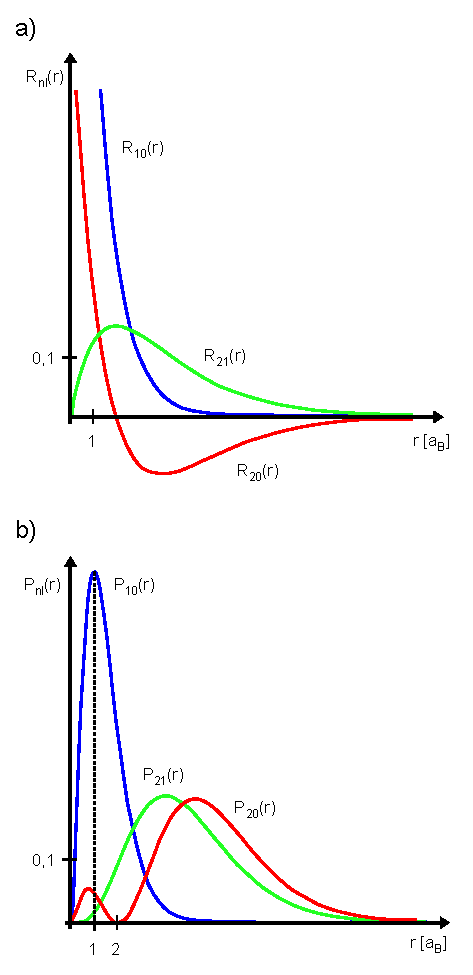
\includegraphics[scale=1]{vodik.pdf}
\caption[Radiální část vlnové funkce]{Na panelu a) jsou vyneseny 3 radiální části vlnové funkce $R_{10}$, $R_{20}$ a $R_{21}$ pro atom vodíku v~závislosti na souřadnici $r$, která je udaná v~jednotkách Bohrova poloměru $a_B$. Na panelu b) jsou vyneseny radiální hustoty pravděpodobnosti $P_{10}$, $P_{20}$ a $P_{21}$. Povšimněme si, že základní stav atomu vodíku $P_{10}$ má maximum hustoty ve vzdálenosti Bohrova poloměru $a_B$.}
\label{obr:RadialniFunkceVodik}
\end{figure}

\clearpage
\section{Přibližné metody}
\label{kap:pribliznemetody}
V~minulých oddílech jsme si ukázali řešení Schr\"{o}dingerovy rovnice pro některé jednoduché případy. Analyticky řešitelných úloh je ale velmi málo. Obecně nejsme schopni (ani v~klasické mechanice) řešit úlohy s~více než dvěma částicemi. Jsme pak odkázáni na řešení přibližná. V~této kapitole si představíme nejdůležitější přibližné přístupy, se kterými se v~kvantové chemii setkáváme.

\subsection{Variační princip}

Přírodní zákony mohou být často formulovány různými způsoby. Principy klasické mechaniky lze například formulovat pomocí soustavy diferenciálních rovnic (např. Newtonových), ale stejně platný je tzv. princip minimálního účinku. Podobně zákony klasické optiky můžeme formulovat pomocí zákonů odrazu a lomu, ale stejně dobře pomocí tzv. Fermatova principu, dle kterého se paprsek mezi dvěma body pohybuje po dráze, na které stráví nejkratší čas. Fermatův princip je příkladem variačního principu. S~variačním principem se hojně setkáváme také v~kvantové mechanice. 

\subsubsection{Variační princip v~kvantové mechanice}

Dle variační teorému je vlastní hodnota Hamiltoniánu pro jakoukoli přibližnou normovanou vlnovou funkci větší nebo rovna energii základního stavu systému:

\begin{equation}
\int\phi^*\hat{H}\phi d\tau\geq E_0,
\label{rov:aprox-variacniteorem}
\end{equation}

\noindent kde $ \phi $ je přibližná vlnová funkce a $ E_0 $ energie základního stavu. Toto tvrzení je nesmírně užitečné. Představme si, že jsme nějakým způsobem odhadli přibližné řešení Schr\"{o}dingerovy rovnice. Variační princip nám umožní rozhodnout, zda toto naše řešení je lepší nebo horší než nějaké jiné přibližné řešení: správnější bude řešení s~nižší energií. Jak uvidíme níže, variační princip nám navíc umožňuje přibližné řešení efektivně nalézt. 


 Ukažme si nyní, že variační princip je ekvivalentní se Schr\"{o}dingerovou rovnicí. Neznámou vlnovou funkci můžeme zapsat ve tvaru lineární kombinace vlastních funkcí Hamiltonova operátoru:

\begin{equation}
\phi=\sum_k c_k \psi_k. 
\label{rov:aprox-rozvojbaze}
\end{equation}

\noindent Připomeňme si zde, že vlastní funkce Hamiltonova operátoru vytváří úplný soubor funkcí, takže výše uvedený rozvoj můžeme určitě udělat. Rozvoj nyní dosadíme do levé strany rovnice \ref{rov:aprox-variacniteorem}: 
\begin{equation}
\int\phi^*\hat{H}\phi d\tau=\int\left( \sum_k c_k^* \psi_k^*\hat{H}\sum_l c_l\psi_l\right)d\tau =\sum_k \sum_l c_k^*c_l\int\psi_k^*\hat{H}\psi_l d\tau=\sum_k \sum_l c_k^*c_lE_k\delta_{kl}.
\end{equation}

\noindent Rovnici si nyní můžeme přepsat do jednoduššího tvaru:
\begin{equation}
\int\phi^*\hat{H}\phi d\tau=\sum_k |c_k|^2E_k.
\label{rov:aprox-vari2}
\end{equation}

\noindent Protože je naše funkce $ \phi $ normovaná, platí $\sum_k |c_k|^2=1 $. Z~definice přitom platí, že $E_0 \leq E_1 \leq E_2$ atd. Tudíž výraz \ref{rov:aprox-vari2} bude určitě větší než $ E_0 $, což není nic jiného než variační teorém.

Při praktickém použití uvažujeme většinou  přibližnou vlnovou funkci závisející na několika parametrech. Minimalizace variačního integrálu

\begin{equation}
\epsilon=\frac{\int\phi^*\hat{H}\phi d\tau}{\int\phi^*\phi d\tau}\geq E_0
\label{rov:aprox-variacniintegrál}
\end{equation}

\noindent vůči těmto parametrům pak umožní nalezení jejich optimálních hodnot. Jmenovatel ve výše uvedeném výrazu je samozřejmě pro normované funkce $ \phi $ jednotkový.

\begin{priklad}
 Použití variačního principu si ukážeme na příkladu jednorozměrné potenciálové jámy. Analytické řečení této úlohy vede k~hodnotám energie $ E_n=\frac{n^2h^2}{8mL^2}$. Přibližná vlnová funkce musí splňovat okrajové podmínky, tedy $ \phi(0)=0 $ a $ \phi(L)=0 $. Nejjednodušší takovou funkcí bude nejspíš kvadratická funkce. Nechť má tedy přibližná funkce $\phi$ následující tvar:
 
\begin{displaymath} 
\phi=x(L-x).
\end{displaymath}
 
Funkce $\phi$ není normovaná, proto nejprve určíme normu:
 
\begin{displaymath} 
N=\int_0^L \phi^*\phi dx=\int_0^L (x(L-x))^2 dx=\frac{L^5}{30} 
\end{displaymath}
 
 Normovaná přibližná funkce tedy vypadá následovně,
 
\begin{displaymath} 
\sqrt{\frac{30}{L^5}} x(L-x).
\end{displaymath}
 
 Připomeňme si ještě, jak vypadá Hamiltonián pro částici v~jednodimenzionální potenciálové jámě:
 
   \begin{displaymath} 
\hat{H}=\frac{-\hbar^2}{2m}\frac{d^2}{d x^2}.
\end{displaymath}
 
Nyní můžeme uplatnit vztah \ref{rov:aprox-variacniteorem}:

   \begin{displaymath} 
E_k=\int\phi^*\hat{H}\phi dx=\frac{-\hbar^2}{2m}\frac{30}{L^5}\int_0^L x(L-x)\left(\frac{d^2 [x(L-x)]}{d x^2}\right)dx
\end{displaymath}
 
 Po vyčíslení dostaneme:
 
    \begin{displaymath} 
E_k=\frac{5h^2}{4\pi^2 mL^2}\geq \frac{h^2}{8mL^2}=E_0.    
\end{displaymath}
 
Na konkrétním příkladu jsme si tak ukázali platnost variačního teorému. 
 \end{priklad}
 
 \subsubsection{Rayleighova-Ritzova metoda}
 
 V~kvantové chemii je užitečné hledat řešení jako lineární kombinaci předem definovaných funkcí a optimalizovat pouze příspěvky jednotlivých bázových funkcí k~celkové vlnové funkci, tj. optimalizovat tzv. rozvojové koeficienty. Tak v~chemii jsme si kupříkladu navykli hledat molekulové orbitaly jako lineární kombinace atomových orbitalů. Zapišme tedy vlnovou funkci pomocí lineární kombinace bázových funkcí:
 
 \begin{equation}
 \phi=\sum_k c_k f_k,
 \label{rov:aprox-Rayleigh-Ritz} 
 \end{equation}
 
\noindent kde $ f_k $ je sada nám známých vhodných funkcí a $ c_k $ jsou rozvojové koeficienty. Ty budeme variačně optimalizovat. Takto definovanou vlnovou funkci nyní dosadíme do výrazu variačního integrálu, \ref{rov:aprox-variacniintegrál}:
 
 \begin{equation}
\epsilon=\frac{\int\sum_k c_k f_k\hat{H}\sum_l c_l f_l d\tau}{\int\sum_k c_k f_k\sum_l c_l f_l d\tau}=\frac{\sum_{k,l} c_k c_l \int f_k \hat{H} f_ld\tau}{\sum_{k,l} c_k c_l \int f_k f_ld\tau}.
\label{rov:aprox-variacniintegrál2}
\end{equation}
 
 \noindent Definujme si nyní matici překryvu \textit{S}:
 \begin{equation}
 S_{kl}=\int f_k f_ld\tau
\end{equation}  
 
\noindent  a Hamiltonovu matici \textit{H}
 
  \begin{equation}
 H_{kl}=\int f_k \hat{H} f_ld\tau,
\end{equation}  
 
 \noindent Variační integrál pak nabude tvaru:
 
   \begin{equation}
 \epsilon=\frac{\sum_{k,l}c_k c_l H_{kl}}{\sum_{k,l}c_k c_l S_{kl}}.
\end{equation}  
 
 \noindent Nejlepší řešení dostaneme pro funkci, pro který bude variační integrál minimální. To vede k~podmínce:
 \begin{equation}
 \frac{\partial \epsilon}{\partial c_i}=0.
 \label{rov:aprox-derivace} 
 \end{equation}
 
 \noindent Derivaci čitatele si rozepíšeme následovně:
 
 \begin{equation}
 \frac{\partial}{\partial c_i} \sum_{k,l}c_k c_l H_{kl}=\sum_{k,l} \frac{\partial}{\partial c_i} (c_k c_l H_{kl})=\sum_{k,l} \left(\frac{\partial c_k}{\partial c_i}c_l H_{kl} + \frac{\partial c_l}{\partial c_i}c_k H_{kl} \right)
   \end{equation}
 
\noindent  Derivace jednotlivých členů se dále zjednoduší, uvažujeme-li:
  \begin{equation}
 \frac{\partial c_k}{\partial c_i}=\delta_{ki}.
   \end{equation}
 
 \noindent Dostaneme tak konečný výraz pro derivaci čitatele z~rovnice \ref{rov:aprox-derivace}:
 
  \begin{equation}
 \frac{\partial}{\partial c_i} \sum_{k,l}c_k c_l H_{kl}=\sum_{k} c_k H_{ki}+\sum_{l} c_l H_{li}.
   \end{equation}
 
 \noindent Použitím posledního vztahu a uplatněním vztahu pro derivaci podílu nakonec dostaneme upravený tvar rovnice \ref{rov:aprox-derivace}:
 
  \begin{equation}
 \frac{\partial\epsilon}{\partial c_i}=\frac{\sum_{k} c_k H_{ki}+\sum_{l} c_l H_{li}}{\sum_{k,l}c_kc_lS_{kl}}-\frac{\left(\sum_{k} c_k S_{ki}+\sum_{l} c_l S_{li}\right)\sum_{k,l}c_k c_l H_{kl}}{\left(\sum_{k,l}c_k c_l\right)^2}
   \end{equation}
 
 \noindent Protože hledáme minimum funkce, položíme variační integrál roven nule (použili jsme znovu definice variačního integrálu \ref{rov:aprox-variacniintegrál2}):
 
  \begin{equation}
 \frac{\partial\epsilon}{\partial c_i}=\frac{\sum_k c_{k}\left(H_{ik}-\epsilon S_{ik}\right)+\sum_l c_{l}\left(H_{li}-\epsilon S_{li}\right)}{\sum_{k,l}c_k c_l}=0
     \end{equation}
 Jelikož na označení sčítacího indexu v~sumě nezáleží, změní se poslední výraz na 
\begin{equation} 
 \frac{\partial\epsilon}{\partial c_i}=\frac{2\sum_k c_{k}\left(H_{ik}-\epsilon S_{ik}\right)}{\sum_{k,l}c_k c_l}=0
\end{equation}
 
\noindent Derivace bude nulová, pokud je nulový čitatel. Tím dostáváme soustavu tzv. sekulárních rovnic:

  \begin{equation}
 \sum_k c_{k}\left(H_{ik}-\epsilon S_{ik}\right)=0
     \end{equation}
 
Jde o~soustavu lineárních rovnic, jejímž řešením jsou rozvojové koeficienty $c_k$. To ovšem za předpokladu, že známe $\epsilon$. To je ale hodnota, kterou hledáme! Všimněme si, že jedno řešení známe okamžitě $c_k=0$. Jde o~tzv. triviální řešení. To nás ale nezajímá, nulové řešení totiž nepředstavuje vlnovou funkci. Lineární algebra nás učí, že soustava rovnic s~nulovou pravou stranou má netriviální řešení pouze tehdy, jestliže je determinant soustavy (v~tomto případě sekulární determinant) nulový:
 
   \begin{equation}
 |H_{ik}-\epsilon S_{ik}|=0
     \end{equation}
 
Sekulární determinant představuje algebraickou rovnici pro neznámou hodnotu $\epsilon$. Pro rozvoj  vlnové funkce do dvou bázových funkcí půjde o~rovnici kvadratickou, pro rozsáhlejší rozvoje půjde o~rovnice vyšších řádů. 
 
 \begin{priklad}
 Použití variačního principu si ukážeme na zápisu molekulového orbitalu homodiatomika (např. H$_{2}$) jako lineární kombinace dvou atomových orbitalů (A~a B) ležících na jednotlivých atomech:  
  \begin{displaymath} 
\phi = c_A\chi_A+c_B\chi_B.    
\end{displaymath}
Nyní si můžeme vyčíslit maticové elementry $H_{kl}$ a $S_{kl}$:

\begin{eqnarray}
H_{AB}&=&\int \chi_A\hat{H}\chi_Bd\tau\nonumber\\
H_{AA}&=&\int \chi_A\hat{H}\chi_Ad\tau=H_{BB}\nonumber\\
S_{AB}&=&\int \chi_A \chi_B d\nonumber\tau
\end{eqnarray}   

Dalším krokem bude sestavení sekulárního determinantu:
 \begin{displaymath}
    \left|\begin{array}{cc@{\quad}r}
     H_{AA} -\epsilon & H_{AB}-\epsilon S_{AB}  \\
     H_{AB} -\epsilon S_{AB} & H_{BB}-\epsilon  \\
    \end{array}\right |=0.
    \end{displaymath}

Sekulární determinant posléze vyřešíme a dostaneme vztah pro $\epsilon$:

\begin{displaymath}
\epsilon_{1,2}=\frac{H_{AA}\pm H_{AB}}{1\pm S_{AB}}.
\end{displaymath}

Dále vyřešíme sekulární rovnice:
\begin{eqnarray}
c_A(H_{AA}-\epsilon S_{AA})+c_B(H_{AB}-\epsilon S_{AB})&=&
c_A(H_{AA}-\epsilon)+c_B(H_{AB}-\epsilon S_{AB})=0\nonumber\\
c_A(H_{BA}-\epsilon S_{BA})+c_B(H_{BB}-\epsilon S_{BB})&=&
c_A(H_{AB}-\epsilon S_{AB})+c_B(H_{AA}-\epsilon)=0.\nonumber
\end{eqnarray}

Do sekulárních rovnic si dosadíme vztahy za $ \epsilon_{1,2} $
a po vyčíslení dostaneme pro  $c_A=c_B$ (pro $ \epsilon_1 $) a $c_A=-c_B$ (pro $ \epsilon_2 $). Ze dvou atomových orbitalů tedy dostaneme vazebný molekulový orbital $ \phi_1 $:
\begin{displaymath}
\phi_1=c_A(\chi_A+\chi_B)
\end{displaymath}
a antivazebný molekulový orbital $ \phi_2 $:
\begin{displaymath}
\phi_2=c_A(\chi_A-\chi_B).
\end{displaymath}
\end{priklad}
 
\begin{priklad}
Jednodimenzionální potenciálovou jámu si nyní vyřešíme i pomocí bázového rozvoje \ref{rov:aprox-Rayleigh-Ritz}. Vlnovou funkci definujeme ve tvaru $ \phi=c_1x^2(L-x)+c_2x(L-x)^2 $. Postup je následující:

\begin{itemize}

\item Spočítáme všechny integrály $H_{k,l}$ a $S_{k,l}$
\item Položíme sekulární determinant roven nule a vypočítáme energie $\epsilon$
\item Pro každou hodnotu $\epsilon$ vypočítáme rozvojové koeficienty ze sekulárních rovnic

\end{itemize}

Příklad vyřešený v~programu Mathematica je dostupný na webových stránkách předmětu.

\end{priklad} 
 
\subsection{Poruchová teorie}
\label{kap:PoruchovaTeorie}
 
Předpokládejme, že řešíme Schrödingerovy rovnici pro nějaký složitý problém:

\begin{equation}
\hat{H}\psi_n=E_n \psi_n,
\end{equation}


\noindent Známe přitom řešení jednoduššího problému, který se od původního problému moc neliší:
 
\begin{equation}
\hat{H}^{(0)}\psi_n^{(0)}=E_n^{(0)} \psi_n^{(0)}.
\end{equation}
 
\noindent Jinými slovy, od jednoduchého problému přejdeme k~problému složitějšímu přidáním malé poruchy. K~řešení problémů tohoto typu používáme poruchovou teorii.
 
\begin{priklad} 
Chceme popsat vibraci molekuly v~anharmonickém potenciálu s~kubickým a kvartickým členem:
  
\begin{equation}
\hat{H}=-\frac{\hbar^2}{2m}\frac{d^2}{dx^2}+\frac{1}{2}kx^2+cx^3+dx^4
\nonumber
\end{equation}
 
Přičemž jsme schopni vyřešit problém pro harmonický potenciál:
 
\begin{equation}
\hat{H}^{(0)}=-\frac{\hbar^2}{2m}\frac{d^2}{dx^2}+\frac{1}{2}kx^2.
\nonumber
\end{equation}
 
Hamiltonián harmonického systému tak representuje neporušený systém a kubické a kvartické členy jsou malá porucha:
 
\begin{equation}
\hat{H}=\hat{H}^{(0)}+cx^3+dx^4.
\end{equation}

Doufáme přitom, že se řešení pro systém s~neporušený systém nebude dramaticky lišit od plného řešení, které získáme malou korekcí neporušeného řešení.
\end{priklad}

Obecně si tedy Hamiltonián definujeme pomocí přibližného Hamiltoniánu a poruchy:

\begin{equation}
\hat{H}=\hat{H}^{(0)}+\lambda\hat{H}',
\end{equation}

\noindent přičemž $ \lambda $ je parametr sloužící k~postupnému zapnutí poruchy ($ \lambda = 0 $ znamená, že máme neporušený systém, $ \lambda=1 $ je naopak plně zapnutá porucha).

Protože Hamiltonián závisí na poruchovém parametru $\lambda$, bude na poruše záviset také vlnová funkce a energie. Vlnovou funkci a energii si rozepíšeme ve formě Taylorova rozvoje okolo poruchového parametru:

\begin{equation}
\psi_{n}=\psi^{(0)}_{n}+\lambda \psi^{(1)}_{n}+\lambda^2 \psi^{(2)}_{n}+...
\label{rov:aprox:poruchawf}
\end{equation}

\begin{equation}
E_{n}=E^{(0)}_{n}+\lambda E^{(1)}_{n}+\lambda^2 E^{(2)}_{n}+...
\end{equation}

V~dalším odvození budeme pracovat s~tím, že vlnová funkce neporušeného systému $\psi^{(0)}_n$ je normalizovaná:
\begin{equation}
\left <\psi^{(0)}_n |\psi^{(0)}_n\right >=1.
\end{equation}
Místo uvažování normalizované vlnové funkce se všemi poruchami budeme uvažovat následující normalizační relaci:

\begin{equation}
\left <\psi^{(0)}_n |\psi_n\right >=1.
\label{rov:aprox:IntermediateNormalization}
\end{equation}

\noindent Tímto způsobem nebude celková poruchová vlnová funkce normalizovaná. To ale nevadí, protože vynásobení vlnové funkce konstantou (normou) nemá vliv na hodnotu energie ze Schrödingerovy rovnice $ \hat{H}\psi_n=E_n\psi_n $. Nyní do normalizační podmínky (\ref{rov:aprox:IntermediateNormalization}) dosadíme poruchovou vlnovou funkci \ref{rov:aprox:poruchawf}:

\begin{equation}
1=\left <\psi^{(0)}_n |\psi^{(0)}_n \right >+
\lambda \left <\psi^{(0)}_n |\psi^{(1)}_n \right >+
\lambda^2 \left <\psi^{(0)}_n |\psi^{(2)}_n \right > + ...
\end{equation}

První člen pravé strany poslední rovnice je jednotkový, protože vlnová funkce neporušeného systému je normalizovaná. Proto musí být další členy nulové:

\begin{eqnarray}
\left <\psi^{(0)}_n |\psi^{(1)}_n \right >=0\\
\left <\psi^{(0)}_n |\psi^{(2)}_n \right >=0. 
\end{eqnarray}

\noindent Nyní si Hamiltonián, energii i vlnovou funkci dosadíme do Schrödingerovy rovnice:

\begin{eqnarray}
\lefteqn{ \left(\hat{H}^{(0)}+\lambda \hat{H}'\right)\left(\psi^{(0)}_{n}+\lambda \psi^{(1)}_{n}+\lambda^2 \psi^{(2)}_{n}+...\right)=}
\nonumber\\
&&=\left(E^{(0)}_{n}+\lambda E^{(1)}_{n}+\lambda^2 E^{(2)}_{n}+...\right)\left(\psi^{(0)}_{n}+\lambda \psi^{(1)}_{n}+\lambda^2 \psi^{(2)}_{n}+...\right)
\end{eqnarray}

\noindent Vytkneme-li z~poslední rovnice člen $\lambda^n$, můžeme si nyní rovnici přepsat do následujícího tvaru:

\begin{eqnarray}
\lefteqn{ \lambda^0\left(\hat{H}^{(0)}\psi^{0}_{n}-E^{(0)}_{n}\psi^{(0)}_{n}\right)+
\lambda^1\left(\hat{H}^{(0)}\psi^{(1)}_{n}+\hat{H}'\psi^{(0)}_{n}-E^{(0)}_{n}\psi^{(1)}_{n}-E^{(1)}_{n}\psi^{(0)}_{n}\right)+{}}
\nonumber\\
&& + 
\lambda^2\left(\hat{H}^{(0)}\psi^{(2)}_{n}+\hat{H}'\psi^{(1)}_{n}+E^{(0)}_{n}\psi^{(2)}_{n}-E^{(1)}_{n}\psi^{(1)}_{n}-E^{(2)}_{n}\psi^{(0)}_{n}\right)+...=0.
\end{eqnarray}

\noindent Vzhledem k~tomu, že rovnice musí platit pro libovolnou hodnotu parametru $\lambda$, musí se každá závorka zároveň rovnat nule. Schrödingerova rovnice se tedy rozpadá na následující rovnice:

\begin{eqnarray}
\hat{H}^{(0)}\psi^{(0)}_{n} &=&E^{(0)}_{n}\psi^{(0)}_{n}\\
\left(\hat{H}^{(0)}-E^{(0)}_{n}\right)\psi^{(1)}_{n} &=&\left(E^{(1)}_{n}-\hat{H}'\right)\psi^{(0)}_{n}
\label{rov:aprox-lambda1} 
\\
\left(\hat{H}^{(0)}-E^{(0)}_{n}\right)\psi^{(2)}_{n} &=&E^{(2)}_{n}\psi^{(0)}_{n}+\left(E^{(1)}_{n}-\hat{H}'\right)\psi^{(1)}_{n}
\end{eqnarray}

Nyní si odvodíme, jak bude vypadat korekce k~energii z~prvního řádu poruchové metody. Využijeme rovnice \ref{rov:aprox-lambda1} Předpokládejme, že funkce $\psi_n^{(0)}$ tvoří úplnou bázi.
Rovnici \ref{rov:aprox-lambda1} nyní vynásobíme komplexně sdruženou funkcí $ \psi_m^{(0)*} $ a přepíšeme do braketové notace:

\begin{equation}
\left < \psi_m^{(0)}|\hat{H}^{(0)}|\psi_n^{(1)} \right >-
E_n^{(0)}\left < \psi_m^{(0)}|\psi_n^{(1)} \right >=
E_n^{(1)}\left < \psi_m^{(0)}|\psi_n^{(0)} \right >-
\left < \psi_m^{(0)}|\hat{H}'|\psi_n^{(0)} \right >.
\label{rov:aprox:poruchaenergie1}
\end{equation}

\noindent První člen v~předchozí rovnici si můžeme upravit s~využitím hermiticity operátoru $\hat{H}^{(0)}$:
\begin{equation}
\left < \psi_m^{(0)}|\hat{H}^{(0)}|\psi_n^{(1)} \right >=
\int \psi_m^{(0)*}\hat{H}^{(0)}\psi_n^{(1)}d\tau=
\int \psi_n^{(1)}\hat{H}^{(0)}\psi_m^{(0)*}d\tau=
E_m^{(0)}\left < \psi_m^{(0)}|\psi_n^{(1)} \right >.
\end{equation}

\noindent Rovnice \ref{rov:aprox:poruchaenergie1} pak přejde na tvar
\begin{equation}
\left(E_m^{(0)}-E_n^{(0)}\right)\left < \psi_m^{(0)}|\psi_n^{(1)} \right >=
E_n^{(1)}\left < \psi_m^{(0)}|\psi_n^{(0)} \right >-
\left < \psi_m^{(0)}|\hat{H}'|\psi_n^{(0)} \right >.
\label{rov:aprox:poruchaenergie2}
\end{equation}

\noindent Nyní mohou nastavit dva případy:
\begin{itemize}
\item $m=n$:
Pokud $m=n$, dostaneme okamžitě korekci k~energii:


\begin{equation}
E_n^{(1)}=\left < \psi_n^{(0)}|\hat{H}'|\psi_n^{(0)} \right >
\label{rov:PorusenaEnergie}
\end{equation} 

Porucha energie v~prvním stupni tedy odpovídá poruše zprůměrované přes neporušenou vlnovou funkci.

\item $m \neq n$:
rovnice \ref{rov:aprox:poruchaenergie2} v~tomto případě přejde na tvar
\begin{equation}
\left(E_m^{(0)}-E_n^{(0)}\right)\left < \psi_m^{(0)}|\psi_n^{(1)} \right >=
-\left < \psi_m^{(0)}|\hat{H}'|\psi_n^{(0)} \right >.
\end{equation}
 Poruchu ve vlnové funkci prvního řádu si vyjádříme jako lineární kombinaci bázových funkcí:

\begin{equation}
\psi_n^{(1)}=\sum_i c_i \psi^{(0)}_i, 
\end{equation}

dále dostaneme

\begin{equation}
\left(E_m^{(0)}-E_n^{(0)}\right)\sum_i c_i\left < \psi_m^{(0)}| \psi^{(0)}_i \right >=
-\left < \psi_m^{(0)}|\hat{H}'|\psi_n^{(0)} \right >
\end{equation}

a po úpravě 

\begin{equation}
\left(E_m^{(0)}-E_n^{(0)}\right) c_m=
-\left < \psi_m^{(0)}|\hat{H}'|\psi_n^{(0)} \right >.
\end{equation}

Korekci prvního řádu k~vlnové funkci tedy dostaneme pomocí následujícího vztahu 

\begin{equation}
\psi_n^{(1)}=\sum_m \frac{\left < \psi_m^{(0)}|\hat{H}'|\psi_n^{(0)} \right >}{E_n^{(0)}-E_m^{(0)}}\psi_m^{(0)}.
\end{equation} 

\end{itemize}

Podobným způsobem, jaký jsme si zde ukázali pro korekce prvního řádu k~energii a vlnové funkci lze odvodit i vztahy pro vyšší řády poruchové energie. Zde uvedeme pouze konečný vztah pro energii s~poruchou druhého řádu:

\begin{eqnarray}
E_n\approx E_n^{(0)}+H'_{nn}+\sum_{m\neq n} \frac{\left | H'_{mn} \right |^2}{E_n^{(0)}-E_m^{(0)}},
\label{rov:aprox:energiePT2}
\end{eqnarray}

\noindent kde $H'_{mn}=\left < \psi_m^{(0)}|H'|\psi_n^{(0)}\right >$. Jistý problém zde představuje skutečnost, že k~výpočtu poruchové energie potřebujeme znát celé spektrum (tj. energii základního i všech excitovaných stavů) energií neporušeného systému. To je v~mnoha případech značně nepraktický požadavek. Pokud víme, jak energie systému přibližně vypadají, můžeme v~některý případech nahradit sumu ve jmenovateli rovnice \ref{rov:aprox:energiePT2} průměrnou excitační energii a dospět k~uzavírací aproximaci (??? CLOSURE APPROXIMATION), která dále zjednodušší tvar rovnice pro energii. 

Poslední problém, jemuž jsme se zde nevěnovali jsou degenerované stavy. Pro degenerované stavy poruchová teorie, jak jsme si ji zde formulovali neplatí, protože člen $E_m^{(0)}-E_n^{(0)}$ bude nulový a vztahy pro rozvojové koeficienty $c_i$ budou divergovat. Pro degenerované vztahy existuje mírně odlišná formulace poruchové teorie, kterou je možné najít v~odborné literatuře. 








\clearpage
\section{Více-elektronové atomy}
\label{kap:viceelektron}
Atom vodíku je asi nejsložitější soustava, kterou jsme schopni analyticky přesně vyřešit. Tato situace je pro chemika pochopitelně málo uspokojivá. Pomocí kvantové teorie bychom chtěli zkoumat vlastnosti atomů a molekul, ve kterých se pohybuje mnoho elektronů! Příslušné Schr\"odingerovy rovnice jsou ale příliš komplikované, takže nejsme schopni naleznout řešení analytické a bohužel ani řešení numericky přesné. Nezbývá nám proto než se vydat do kalných vod přibližných metod. Řešení Schr\"odingerovy rovnice pro atom vodíku nám nicméně poskytne dobrý základ, ze kterého je možné se odrazit k~přibližnému řešení problému více-elektronových atomů. Základní postupy si můžeme ukázat již na \uv{nejjednodušším složitém atomu}, atomu helia.  

\subsection{Atom helia}
V~atomu helia na sebe působí tři částice, jádro helia s~protonovým (resp. nábojovým) číslem $Z = 2$ a dva elektrony. Nebude nám tudíž zatěžko napsat pro helium hamiltonián 

\begin{equation}
\hat{H} = - \frac{\hbar^2}{2 m_e} \left( \Delta e_1 + \Delta e_2 \right) - \frac{1}{4 \pi \epsilon_0} \left(\frac{2e^2}{r_1} + \frac{2e^2}{r_2} \right) + \frac{1}{4 \pi \epsilon_0} \frac{e^2}{r_{12}},
\label{rov:VE-1}
\end{equation}


\noindent kde hamiltonián zapisujeme v~souřadnicové soustavě umístěné do jádra helia.
\begin{equation}
\Delta_{e_1} \equiv \frac{\partial^2}{\partial x_{e1}^2} + \frac{\partial^2}{\partial y_{e1}^2}+\frac{\partial^2}{\partial z_{e1}^2} \nonumber
\end{equation}
je Laplaceův operátor prvního elektronu popisující kinetickou energii prvního elektronu,
\begin{equation}
\Delta_{e_2} \equiv \frac{\partial^2}{\partial x_{e2}^2} + \frac{\partial^2}{\partial y_{e2}^2}+\frac{\partial^2}{\partial z_{e2}^2} \nonumber
\end{equation}
je Laplaceův operátor příslušející druhému elektronu, $r_1$ je vzdálenost mezi jádrem helia a~prvním elektronem, $r_2$ je vzdálenost mezi jádrem helia a druhým elektronem,a $r_{12}$ je vzdálenost mezi oběma elektrony. Schr\"odingerova rovnice je v~tomto případě parciální diferenciální rovnicí druhého řádu, jejímž řešením je (vlnová) funkce šesti proměnných, kupříkladu kartézských souřadnic obou elektronů $x_1$, $y_1$, $z_1$, $x_2$, $y_2$ a $z_2$ nebo sférických souřadnic těchto elektronů $r_1$, $\theta_1$, $\phi_1$, $r_2$, $\theta_2$, $\phi_2$. Bohužel, ani v~jedné sadě souřadnice se nám nepodaří hamiltonián separovat, nemůžeme jej napsat jakou součet členu závisejících na souřadnicích pouze jednoho elektronu a členu závisejícího pouze na souřadnicích elektronu druhého. Hamiltonián můžeme zapsat následujícím způsobem

\begin{equation}
\hat{H} = \hat{H}_1 + \hat{H}_2 + \hat{H}_{12},
\label{rov:VE-2}
\end{equation}

\noindent kde hamiltonián 

\begin{equation}
\hat{H}_1 = - \frac{\hbar^2}{2 m_e} \Delta_1 - \frac{1}{4 \pi \epsilon_0} \frac{2 e^2}{r_1}
\label{rov:VE-3}
\end{equation} 

\noindent působí toliko na souřadnice prvního elektronu a hamiltonián 

\begin{equation}
\hat{H}_2 = - \frac{\hbar^2}{2 m_e} \Delta_2 - \frac{1}{4 \pi \epsilon_0} \frac{2 e^2}{r_2}
\label{rov:VE-4}
\end{equation}

\noindent pouze na souřadnice elektronu druhého. Problém působí člen popisující odpuzování mezi elektrony 

\begin{equation}
\hat{H}_{12} = \frac{1}{4 \pi \epsilon_0} \frac{e^2}{r_{12}} = \frac{1}{4 \pi \epsilon_0} \frac{e^2}{\vert \vec{r_1} - \vec{r_2} \vert}. 
\label{rov:VE-5}
\end{equation}

Pokud bychom mohli zanedbat tento člen, byla by situace růžová. Celkovou vlnovou funkci pak snadno zapíšeme jako součin dvou vlnových funkcí $\phi_1$ a $\phi_2$ (metoda separace proměnných, srov. rovnici \eqref{rov:2č-nez3}

\begin{equation}
\psi = \phi_1 \cdot \phi_2,
\label{rov:VE-6}
\end{equation}

\noindent přičemž $\phi_1$ závisí pouze na souřadnicích prvního elektronu a je dána řešením rovnice

\begin{equation}
\hat{H}_1 \phi_1 = E_1 \phi_1.
\label{rov:VE-7}
\end{equation}

Tato rovnice ale není než  Schr\"odingerova rovnice pro atom vodíkového typu! Její řešení tudíž známe

\begin{equation}
\phi_1 = \frac{1}{\sqrt{\pi}} \left(\frac{Z}{a_0} \right)^{3/2} e^{-\frac{Z r_1}{a_0}},
\label{rov:VE-8}
\end{equation}

\noindent kde Bohrův poloměr lze vyjádřit pomocí fundamentálních fyzikálních konstant

\begin{equation}
a_0 = \frac{4 \pi \epsilon_0 \hbar^2}{m_e e^2}.
\label{rov:VE-9}
\end{equation}

\noindent Analogické vztahy platí pro vlnovou funkci $\phi_2$, takže celkovou vlnovou funkci můžeme napsat jako 

\begin{equation}
\psi = \phi_1 \cdot \phi_2 = \frac{1}{\pi} \frac{Z^3}{a_0^3} e^{-\frac{Z r_1}{a_0}} e^{-\frac{Z r_2}{a_0}}.
\label{rov:VE-10}
\end{equation}


\noindent Energie atomu helia při zanedbání členu \eqref{rov:VE-5} (tedy při zanedbání odpuzování elektronů) je pak dána vztahem

\begin{equation}
E = E_1 + E_2 = -13{,}6 \left(\frac{Z^2}{n^2} + \frac{Z^2}{n^2} \right) \mbox{ eV} = -13{,}6 \cdot 8 \mbox{ eV} = -108{,}8 \mbox{ eV}.
\label{rov:VE-11}
\end{equation}

Tato hodnota je po čertech vzdálena od hodnoty změřené experimentálně ($-$79,0~eV). Čtenář může být navíc znejistěn skutečností, že vypočítaná hodnota je nižší než hodnota experimentální. Neprotiví se tento výsledek variačnímu principu? Po bližším ohledání zjistíme, že nikoliv. Variační princip praví, že energie vypočítaná s~přibližnou vlnovou funkcí pomocí správného hamiltoniánu je vždy vyšší než energie skutečná. Naše zjednodušení ale nespočívalo v~nalezení přibližné vlnové funkce pro přesný hamiltonián, nýbrž v~nalezení přesného řešení pro přibližný hamiltonián. 

Z~předchozího výpočtu vyplývá, že mezi-elektronové odpuzování v~našich úvahách zanedbat nemůžeme. V~následujících oddílech si ukážeme, kterak elektronovou energii atomu helia vypočítat s~využitím dvou cest, pomocí poruchového i variačního přístupu.

\subsubsection{Výpočet elektronové energie atomu helia poruchovým přístupem}

V~poruchové teorii předpokládáme, že jsme schopni nalézt řešení pro přibližný hamiltonián $\hat{H}^{(0)}$ a pomocí tohoto řešení pak hledáme řešení pro přesný hamiltonián $\hat{H} = \hat{H}^{(0)} + \hat{H}^{\prime}$. Zvolme si jako hamiltonián nultého řádu součet

\begin{equation}
\hat{H}^{(0)} = \hat{H}_1 + \hat{H}_2,
\label{rov:VE-12}
\end{equation}

\noindent ve kterém je zanedbána mezi-elektronové odpuzování. Řešení pro tento systém známe. Korekce prvního řádu pro energii (srov. oddíl \ref{kap:PoruchovaTeorie}, vztah \eqref{rov:PorusenaEnergie}) je pak dána jako

\begin{equation}
E^{(1)} = \int \psi^{(0)} \hat{H}^{\prime} \psi^{(0)} \mathrm{d}\tau,
\label{rov:VE-13}
\end{equation}

\noindent což v~našem případě konkrétně znamená šesti-dimenzionální integraci přes (sférické) souřadnice obou elektronů 

\begin{equation}
E^{(1)} = \frac{1}{4 \pi \epsilon_0} \frac{Z^6 e^2}{\pi^2 a_0^6} \int \limits_0^{2 \pi} \int \limits_0^{2 \pi} \int \limits_0^{\pi} \int \limits_0^{\pi} \int \limits_0^{\infty} \int \limits_0^{\infty} e^{-\frac{Z r_1}{a_0}} e^{-\frac{Z r_2}{a_0}} \frac{1}{r_{12}} r_1^2 \sin \theta_1 r_2^2 \sin \theta_2 \mathrm{d}r_1 \mathrm{d}r_2 \mathrm{d} \theta_1 \mathrm{d}\theta_2 \mathrm{d}\phi_1 \mathrm{d}\phi_2,
\label{rov:VE-14}
\end{equation}
kde jsme za $\psi^{(0)}$ dosadili ze vztahu \eqref{rov:VE-10}. Výrazy $r_1^2 \sin \theta_1$ a $r_2^2 \sin \theta_2$ představují Jakobián transformace z kartézských do sférických souřadnic.

Vyčíslení tohoto integrálu je poněkud svízelné, ale proveditelné. Po provedení získáme korekci prvního řádu. Celková energie v~rámci poruchové metody prvního řádu je tak 

\begin{equation}
E= E^{(0)} + E^{(1)} = -108{,}8 + 34=-74{,}8 \mbox{ eV}.
\label{rov:VE-15}
\end{equation}

Souhlas s~experimentem již tedy není úplně špatný! V~poruchovém metodě bychom mohli pokračovat do vyšších řádů. Pro helium vychází korekce vyšších řádů

\begin{eqnarray*}
E^{(2)} &=& -4{,}3 \mbox{ eV}\\
E^{(3)} &=& 0{,}1 \mbox{ eV}
\end{eqnarray*}

Postupně tak v~rámci poruchové metody konvergujeme k~experimentální hodnotě.

\subsubsection{Výpočet elektronové energie atomu helia variačním přístupem}

Při variačním řešení potřebujeme najít nějakou přibližnou (ale rozumnou) vlnovou funkci, která má nedourčené parametry. Vyjděme z~funkce ve tvaru


\begin{equation}
\Phi = \frac{1}{\pi} \left(\frac{Z^{\prime}}{a_0} \right)^3 e^{-\frac{Z^{\prime} r_1}{a_0}} e^{-\frac{Z^{\prime} r_2}{a_0}}.
\label{rov:VE-16}
\end{equation}

Tato funkce vypadá jako vlnová funkce atomu helia, ve kterém se elektrony neodpuzují. Místo nábojového čísla $Z = 2$ máme ale nyní ve funkci neurčený parametr $Z^{\prime}$. Fyzikálně si můžeme představit, že díky přítomnosti druhého elektronu \uv{vidí} první elektron jádro o~menším náboji, než jaký skutečně má. Jinými slovy, elektrony stíní atomové jádro. Hodnotu parametru $Z^{\prime}$, tj. efektivního náboje jádra, je třeba určit na základě minimalizace energie vzhledem k~parametrům zkusmé funkce. 

Musíme začít vyjádření funkcionál energie, tj. závislosti energie na konkrétní formě zkusmé funkce. Začneme tím, že si hamiltonián  \eqref{rov:VE-1} napíšeme v~mazané formě

\begin{equation}
\hat{H} = \underbrace{\left[ - \frac{\hbar^2}{2 m_e} (\Delta_1 + \Delta_2) - \frac{Z^{\prime} e^2}{4 \pi \epsilon_0 r_1} - \frac{Z^{\prime} e^2}{4 \pi \epsilon_0 r_2} \right]}_{\hat{H}_0^{\prime}} + (Z^{\prime} - Z) \frac{e^2}{4 \pi \epsilon_0 r_1} + (Z^{\prime} - Z) \frac{e^2}{4 \pi \epsilon_0 r_2} - \frac{e^2}{4 \pi \epsilon_0 r_{12}} ,
\label{rov:VE-17}
\end{equation}

\noindent kdy přitom pro hamiltonián $\hat{H}_0^{\prime}$ zjevně platí\footnote{Jde totiž o hamiltonián atomu vodíkového typu, pro nějž řešení známe.}

\begin{equation}
\hat{H}_0^{\prime} \Phi = E^{\prime} \Phi,
\label{rov:VE-18}
\end{equation}
kde
\begin{equation}
E^{\prime} = - \frac{2 (Z^{\prime})^2 e^2}{8 \pi \epsilon_0 a_0}. \nonumber
\end{equation}

\noindent Pro funkcionál energie pak platí

\begin{equation}
E = \int \Phi^{\ast} \hat{H} \Phi \mathrm{d}\tau = E^{\prime} + \frac{e^2}{4 \pi \epsilon_0} \left[ (Z^{\prime} - Z) \int \frac{\Phi^{\ast}\Phi}{r_1} \mathrm{d}\tau + (Z^{\prime} - Z) \int \frac{\Phi^{\ast}\Phi}{r_2} \mathrm{d}\tau + \int \frac{\Phi^{\ast}\Phi}{r_{12}} \mathrm{d}\tau \right],
\label{rov:VE-19}
\end{equation}
což po lehce otravném vyčíslení integrálů vede k výrazu
\begin{equation}
E = \left( (Z^{\prime})^2 - 2 Z Z^{\prime} + \frac{5}{8} Z^{\prime} \right) \frac{e^2}{4 \pi \epsilon_0 a_0}.
\label{rov:VE-20}
\end{equation}

\noindent Všimněme si, že ve funkcionálu energie nám vystupuje jak nábojové číslo $Z$ (z~hamiltoniánu, nejde o~variační parametr), tak efektivní nábojové číslo $Z^{\prime}$. Optimální hodnotu $Z^{\prime}$ nalezneme jako minimum funkcionálu energie, tj. položením derivace tohoto funkcionálu nule

\begin{equation}
2 Z^{\prime} - 2Z + \frac{5}{8} = 0 \nonumber
\end{equation}

\noindent z~čehož po dosazení $Z = 2$

\begin{equation}
Z^{\prime} = 1{,}6875. \nonumber
\end{equation}

\noindent Po dosazení optimální hodnoty $Z^{\prime}$ do funkcionálu energie dostaneme hodnotu 

\begin{equation}
E = \left( (1{,}6875)^2 - 2 \cdot 2 \cdot 1{,}6875 + \frac{5}{8} \cdot 1{,}6875 \right) \frac{e^2}{4 \pi \epsilon_0 a_0} = - 77{,}48 \mbox{ eV}.
\label{rov:VE-21}
\end{equation}

\noindent To je však již hodnota energie, která je ve velmi slušném souladu s~experimentem. Mohli bychom tuto hodnotu ještě nějak vylepšit? Nepochybně mohli, ale potřebovali bychom již složitější tvar zkusmé funkce $\Phi$. Její současná forma předpokládá nezávislý pohyb obou elektronů, zanedbává korelaci jejich pohybů. Pokročilejší metody elektronové struktury musí jít za rámec této aproximace. O~tom se dozvíme více v~oddílu o~metodách popisu elektronové struktury molekul. 

\subsection{Atomy o~více než dvou elektronech}
Poté, co jsme se naladili úspěchem kvantových výpočtů pro atom helia, můžeme být v~pokušení uplatnit celý postup i na další atomy. Vezměmež si třeba atom lithia. Zde zkusmou vlnovou funkci budeme hledat jako

\begin{equation}
\Phi = \phi_1 \phi_2 \phi_3,
\label{rov:VE-22}
\end{equation}

\noindent přičemž $\phi_i$ bude podobně jako v~případě helia dáno jako

\begin{equation}
\phi_i = \frac{1}{\sqrt{\pi}} \left(\frac{Z^{\prime}}{a_0} \right)^{3/2} e^{-\frac{Z^{\prime r_i}}{a_0}}.
\label{rov:VE-23}
\end{equation}

Výpočet vede k~energii lithia $-$230 eV. Experimentální hodnota je ovšem pouze $-203{,}5$~eV. Tento výsledek se jeví být v~přímém rozporu s~variačním principem. Je snad něco špatně s~variačním principem nebo s~přírodou? Poučený čtenář asi tuší, že problém nastal ignorováním Pauliho vylučovacího  principu. Vlnovou funkci předpokládáme ve formě

\begin{equation}
\psi = 1\mathrm{s}(1) 1\mathrm{s}(2) 1\mathrm{s}(3)
\label{rov:VE-24}
\end{equation}

\noindent neboli

\begin{equation}
1\mathrm{s}^3. \nonumber
\end{equation}

\noindent To není symbol, se kterým bychom se v~učebnicích chemie setkávali. Je třeba na tomto místě ale připomenout, že s~Pauliho principem kvantová mechanika až do této chvíle nepočítala. Je třeba si o~něm říci více.

\subsection{Antisymetrie vlnové funkce a Pauliho vylučovací princip}

Pauliho vylučovací princip zná většina studentů již ze střední školy. Zhruba řečeno nám tvrdí, že dva elektrony se v~atomu (či v~molekule, pevné látce a kdekoliv jinde) nemohou nacházet ve stejném kvantovém stavu. Wolfgang Pauli tento princip formuloval na základě studia atomových spekter jako experimentální skutečnost. Později se teprve objevila souvislost mezi Pauliho vylučovacím principem a obecnými vlastnostmi mnoha-částicové vlnové funkce.    

Kvantově-mechanické částice (jako jsou elektrony) jsou nerozlišitelné, nemůžeme je \uv{obarvit} a sledovat, jak se pohybují. Je to důsledek relací neurčitosti. Pokud bychom pohyb nějaké částice chtěli sledovat, potřebovali bychom vědět polohu částice v~daném čase, ale také její rychlost. Ta nám totiž řekne, kde příslušnou částici můžeme očekávat v~následujícím okamžiku. Obojí informaci ale zároveň nemůžeme získat s~libovolnou přesností, nemá tak smysl mluvit o~trajektorii částice a částice nemůžeme rozlišit. Nemůžeme nijak poznat, pokud se dva elektrony prohodí. V~jazyku kvantové mechaniky nerozlišitelnost částic vyjádříme vztahem

\begin{equation}
\vert \psi(1,2) \vert^2 = \vert \psi(2,1) \vert^2.
\label{rov:VE-25}
\end{equation}

\noindent Tato rovnice nám říká, že pravděpodobnost, že se na místě A~bude nacházet první částice a~na místě B druhá částice, musí být stejná, jako pravděpodobnost nalezení částice 1 na místě B a~částice 2 na místě A. Tato identita může být realizovaná dvěma způsoby

\begin{equation}
\psi(1,2) = \psi(2,1)
\label{rov:VE-26}
\end{equation}

\noindent a

\begin{equation}
\psi(1,2) = - \psi(2,1).
\label{rov:VE-27}
\end{equation}


\noindent V~prvním případě říkáme, že vlnová funkce je symetrická vůči permutaci dvou částic. Částice, které splňují toto pravidlo, se nazývají Boseho částice nebo prostě \textbf{bosony}. Ukazuje se, že jde o~částice s~celočíselnou hodnotou spinu a že pro tyto částice neplatí Pauliho vylučovací princip (viz dále). Naproti tomu částice s~vlnovou funkcí antisymetrickou vůči permutaci částic nazýváme Fermiho částicemi (nebo \textbf{fermiony}). Fermiony mají poločíselný spin a \textbf{Pauliho vylučovací princip} pro ně platí. K~bosonům náleží kupříkladu foton, k~fermionům pak elektron. To, zda je daná částice fermion nebo boson, je dáno experimentálně. V~kvantové mechanice tuto skutečnost zavádíme jako postulát.

\bigskip
\textbf{Postulát číslo 6: Při záměně dvou elektronů musí vlnová funkce změnit znaménko. (Spinově-statistický postulát)}
\bigskip

Ukažme si nyní souvislost mezi antisymetrií vlnové funkce vylučovacím principem. Představme si elektrony, které jsou charakterizovány polohou a průmětem spinu do osy $z$

\begin{equation}
q_i = (\vec{r_1},m_{s,i}).
\label{rov:VE-28}
\end{equation}

\noindent Jelikož jde o~fermiony, musí platit 

\begin{equation}
\psi(q_1,q_2,q_3, \dots q_N) = -\psi(q_2,q_1,q_3, \dots q_N).
\label{rov:VE-29}
\end{equation}

Uvažme nyní situaci, kdy oba elektrony mají přesně stejnou polohu a také stejnou hodnotu projekce spinu, jinými slovy $q_1 = q_2$. Předchozí rovnice pak nabývá tvaru

\begin{equation}
\psi(q_1,q_1,q_3, \dots q_N) = - \psi(q_1,q_1,q_3, \dots q_N),
\label{rov:VE-30}
\end{equation}

\noindent z~čehož ale okamžitě plyne

\begin{equation}
\psi(q_1,q_1,q_3, \dots q_N) = 0
\label{rov:VE-31}
\end{equation}

\noindent Pravděpodobnost, že by se dva elektrony se stejnou projekcí spinu do osy $z$ (nadále budeme užívat výrazu \uv{se stejným spinem}) mohly nacházet na stejném místě je nulová. Toto \uv{odpuzování} elektronů nesouvisí s~elektrostatickými silami, je přímým důsledkem antisymetrie vlnové funkce. Mluvíme o~\textbf{Pauliho repulzi}.

V~našem výkladu atomu helia jsme s~výhodou hledali řešení Schr\"odingerovy rovnice ve tvaru součinu

\begin{equation}
\psi(1,2, \dots N) = \phi_1(1)\phi_2(2) \dots \phi_N(N),
\label{rov:VE-32}
\end{equation}
který pro případ dvou elektronů
\begin{equation}
\psi(1,2) = \phi_1(1) \phi_2(2). \nonumber
\end{equation}

\noindent Takto zapsaná vlnová funkce ale není antisymetrická (dokonce ani ne symetrická, permutací elektronů získáme úplně jinou funkci). Nejjednodušší funkce ve tvaru součinu jedno elektronových funkcí bude mít následující tvar

\begin{equation}
\psi(1,2) = \frac{1}{\sqrt{2}} \left[ \phi_1(1)\phi_2(2) - \phi_1(2)\phi_2(1) \right].
\label{rov:VE-33}
\end{equation}
kde faktor $1/\sqrt{2}$ přidáváme z důvodů normalizace.

\noindent Vlnová funkce dvou elektronů popsaných stejnou jedno-elektronovou funkci (tj. stejným orbitalem $\phi_1 = \phi_2$) ale nezbytně musí být identicky rovna nule

\begin{equation}
\psi(1,2) = \frac{1}{\sqrt{2}} \left[ \phi_1(1)\phi_1(2) - \phi_1(2)\phi_1(1) \right] = 0.
\label{rov:VE-34}
\end{equation}

\noindent Právě toto tvrzení známe z~chemických učebnic jako Pauliho vylučovací princip. Zde vidíme, že tento původně na základě spektroskopických experimentů odvozený princip úzce souvisí s~antisymetrií vlnové funkce. 

Zmiňme na tomto místě, že jedno-elektronová vlnová funkce $\phi$ má svou prostorovou část $\chi$ a spinovou část $\alpha$ $\beta$

\begin{equation}
\phi = \chi \cdot \alpha \mbox{ nebo } \phi = \chi \cdot \beta.
\label{rov:VE-35}
\end{equation}

\noindent Mluvíme pak o~tzv. \textbf{spinorbitalu}. Vlnová funkce atomu helia v~základním stavu by pak vypadala takto

\begin{eqnarray}
\phi_1 &=& 1\mathrm{s} \cdot \alpha \\ \nonumber
\phi_2 &=& 1 \mathrm{s} \cdot \beta \\ \nonumber
\psi &=& \frac{1}{\sqrt{2}} \left[1\mathrm{s}(1) \alpha(1) 1 \mathrm{s}(2) \beta (2) - 1 \mathrm{s}(2) \alpha(2) 1\mathrm{s}(1) \beta(1) \right] = \frac{1}{\sqrt{2}} 1\mathrm{s}(1) 1 \mathrm{s}(2) \left[\alpha(1) \beta (2) - \alpha(2) \beta(1) \right].
\end{eqnarray}

\noindent Celková vlnová funkce je tak dána součinem prostorové části a části spinové. V~hamiltoniánu se ale spin nevyskytuje a my nakonec řešíme Schr\"odingerovu rovnici pouze pro prostorovou část vlnové funkce

\begin{equation}
\hat{H} 1\mathrm{s}(1) 1\mathrm{s}(2) = E 1\mathrm{s}(1) 1 \mathrm{s}(2).
\label{rov:VE-36}
\end{equation}

\noindent Na našich předchozích výpočtech se tak nic nezměnilo. V~případě obecné mnoha-elektronové vlnové funkce spin ignorovat nemůžeme a díky tomu má třeba tripletní stav jinou energii než stav singletní. 

Nejjednodušší obecný tvar antisymetrické vlnové funkce pro $N$-elektronový systém získáme ve formě tzv. \textbf{Slaterova determinantu}

\begin{equation}
\psi = \frac{1}{\sqrt{N!}}
\begin{vmatrix}
\phi_1(1) & \phi_1(2) & \cdots & \phi_1(N) \\
\phi_2(1) & \phi_2(2) & \cdots & \phi_2(N) \\
\vdots & \vdots & \vdots & \vdots \\
\phi_N(1) & \phi_N (2) & \cdots & \phi_N(N)
\end{vmatrix}.
\label{rov:VE-37}
\end{equation}

\noindent Díky vlastnostem determinantu je antisymetrie vlnové funkce automaticky zajištěna. Tvar vlnové funkce \eqref{rov:VE-33} je speciálním případem Slaterova determinantu pro $N=2$. Pro atom lithia bychom zapsali Slaterův determinant ve tvaru

\begin{equation}
\psi = \frac{1}{\sqrt{6}}
\begin{vmatrix}
1 \mathrm{s}1 \alpha(1) & 1 \mathrm{s}(2) \alpha (2) & 1 \mathrm{s}(3) \alpha (3) \\
1 \mathrm{s}1 \beta(1) & 1 \mathrm{s}(2) \beta (2) & 1 \mathrm{s}(3) \beta (3) \\
2 \mathrm{s}1 \alpha(1) & 2 \mathrm{s}(2) \alpha (2) & 2 \mathrm{s}(3) \alpha (3) \\
\end{vmatrix}.
\label{rov:VE-38}
\end{equation}


\noindent Zde již ovšem nemůžeme vlnovou funkci zapsat jako součin prostorové a spinové části. Když nyní budeme v~této formě hledat energii atomu lithia v~rámci poruchového přístupu, získáme

\begin{eqnarray*}
E^{(0)} &=& E_{1s} + E_{1s} + E_{2s} = -275{,}5 \mbox{ eV} \\
E^{(1)} &=& \braket{\psi^{(0)}|\hat{H}^{\prime}|\psi^{(0)}} = 83{,}5 \mbox{ eV}\\
E &=& E^{(0)} + E^{(1)} = -192 \mbox{ eV},
\end{eqnarray*}
kde
\begin{equation}
\hat{H}^{\prime} = \left( \frac{1}{r_{12}} + \frac{1}{r_{13}} + \frac{1}{r_{23}} \right) \frac{e^2}{4 \pi \epsilon_0}.  \nonumber
\end{equation}

\noindent Variačním řešením pak získáme energii

\begin{equation}
E = - 201{,}2 \mbox{ eV}. \nonumber
\end{equation}

\noindent Tedy hodnotu vyšší (ale zároveň relativně blízko) v~porovnání s~hodnotou experimentální, $-203{,}5$~eV. 


\subsection{Hartreeho a Hartreeho-Fockova metoda pro atomy}
 
Zformulujeme nyní obecný způsob, který nám umožní systematickým způsobem řešit Schr\"odingerovu rovnici pro $N$-elektronový atom (a obecně $N$-elektronovou molekulu) pomocí variačního principu. Budeme promýšlet opět případ atomu helia, rozšíření na více-elektronové atomy je ale přímočaré. 

V~předchozích oddílech jsme viděli, že je rozumné hledat vlnovou funkci atomu helia ve formě součinu
 
\begin{equation}
\psi = g_1(r_1, \theta_1, \phi_1) g_2(r_2,\theta_2, \phi_2).
\label{rov:VE-39}
\end{equation}
 
\noindent Z~pohledu teorie pravděpodobnosti nám tato rovnice říká, že pohyb prvního a druhého elektronu je nezávislý. Ne že by se ty dva elektrony \uv{necítily}, nicméně předpokládáme, že elektron \uv{cítí} jenom průměrné pole generované druhým elektronem. Jelikož se v~tomto oddíle zabýváme atomy, budeme pro jednoelektronové vlnové funkce $g_1$ a $g_2$ předpokládat tvar 
  
\begin{eqnarray}
g_1 &=& h_1(r_1) Y_{l_1}^{m_1} (\theta_1,\phi_1) \\
g_2 &=& h_2(r_2) Y_{l_2}^{m_2} (\theta_2,\phi_2),
\end{eqnarray}
  
\noindent kde $Y_{l}^{m}$ jsou sférické harmonické funkce. Předpokládejme nyní, že nám někdo prozradil tvar jedno-elektronové vlnové funkce $g_2$ a nám zbývá dopočítat vlnovou funkci $g_1$. První elektron se bude pohybovat v~elektrostatickém poli jádra helia a dále na něj bude působit druhý elektron, jehož rozložení v~prostoru ale díky znalosti vlnové funkce $g_2$ známe. Můžeme tak předpokládat, že se bude pohybovat v~efektivním potenciálu
  
\begin{equation}
\tilde{V}_1 (r_1, \theta_1,\phi_1) = \frac{e^2}{4 \pi \epsilon_0} \int \frac{\vert g_2 \vert^2}{r_{12}} \mathrm{d}\tau - \frac{Z e^2}{4 \pi \epsilon_0 r_1}.
\label{rov:VE-40}
\end{equation}
  
Udělejme ještě jedno další přiblížení, totiž to, že zprůměrujeme tento potenciál přes úhlové souřadnice a budeme předpokládat, že se elektron pohybuje v~centrálním poli
 
\begin{equation}
V_1(r_1) = \frac{\int_0^{2 \pi} \int_0^{\pi} V_1(r_1,\theta_1,\phi_1) \sin \theta_1 \mathrm{d}\theta_1 \mathrm{d}\phi_1}{\int_0^{2 \pi} \int_0^{\pi} \sin \theta_1 \mathrm{d}\theta_1 \mathrm{d}phi_1}.
\label{rov:VE-41}
\end{equation}
 
 
\noindent Vlnovou funkci $g_1$ pak nalezneme řešením  jedno-elektronové Schr\"odingerovy rovnice
 
\begin{equation}
\underbrace{\left[ - \frac{\hbar^2}{2 m_e} \Delta_1 + V_1(r_1) \right]}_{\hat{h}_1} g_1 = \varepsilon_1 g_1.
\label{rov:VE-42}
\end{equation}
 
Takovouto rovnici už jsme schopni řešit, byť by se tak dělo numerickými metodami. Navíc jde o~rovnici s~centrálně-symetrickým potenciálem, takže bude platit
 
\begin{equation}
[\hat{H},\hat{L}^2] = [\hat{H},\hat{L_z}] = 0
\label{rov:VE-43}
\end{equation}
 
\noindent a velikost momentu hybnosti i projekce momentu hybnosti do jedné z~os se budou zachovávat. Kvantová čísla $l$ a $m$ budou tudíž \uv{dobrá kvantová čísla}. Jedno-elektronové vlnové funkce budou i tentokráte charakterizovány kvantovými čísly $n$, $l$ a $m$, nicméně nebudou již platit degenerace mezi hladinami o~stejném hlavním kvantovém čísle $n$.
 
Máme ale jednu potíž. Celou dobu předpokládáme, že známe vlnovou funkci $g_2$. Jenže my ji ve skutečnosti neznáme! V~rovnici \eqref{rov:VE-42} se nám tak objevuje neznámá funkce $g_2$. Mohli bychom celou úvahu provést i naopak, budeme předpokládat, že známe vlnovou funkci $g_1$ a~budeme se snažit vypočítat vlnovou funkci $g_2$. Dostaneme tak soustavu dvou rovnic pro dvě neznámé funkce, $g_1$ a $g_2$. Jde o~složitou soustavu integro-diferenciálních (a k~tomu nelineárních) rovnic. Řešení pak hledáme iterativním způsobem, pomocí tzv. metody samo-souhlasného pole (SCF, z~angl. \textit{Self-Consistent Field}). Výpočet začneme hrubým odhadem tvaru vlnových funkcí $g_1$ a~$g_2$. Pomocí těchto odhadů vlnových funkcí určíme efektivní pole, ve kterých se oba elektrony pohybují (jinými slovy použijeme tyto funkce ke konstrukci jedno-elektronových hamiltoniánů v~rovnici \eqref{rov:VE-42}). Vyřešením rovnice \eqref{rov:VE-42} získáme novou sadu funkcí $g_1$ a $g_2$. Celé kolečko se může opakovat, do doby, než se funkce již dále nemění (viz obrázek~\ref{obr:SCFcycle}).

\begin{figure} [ht]
\centering
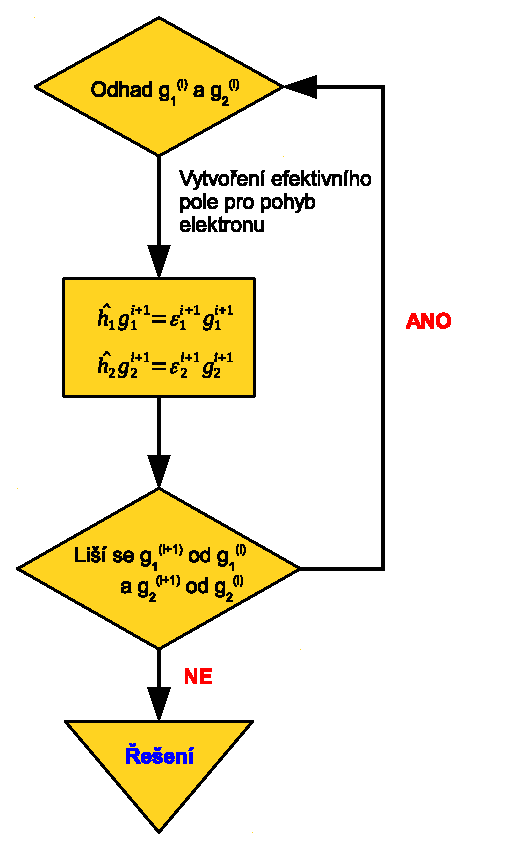
\includegraphics[scale=0.7]{SFCcyklus.eps}
\caption[SCF kolečko]{Řešení Hartreeho a Hartreeho-Fockových rovnice se prakticky provádí iterativním způsobem.}
\label{obr:SCFcycle}
\end{figure}
  
Předvedený postup představuje tzv. Hartreeho metodu. Naše \uv{odvození} bylo heuristické, ke stejnému výsledku bychom ale došli s~použitím variačního počtu. Obecně v~Hartreeho metodě předpokládáme zkusmou vlnovou funkci ve tvaru součinu $N$ jedno-elektronových vlnových funkcí

\begin{equation}
\Phi = q_1 q_2 q_3 \dots q_N.
\label{rov:VE-44}
\end{equation}

\noindent Každý z~elektronů se pak pohybuje v~efektivním potenciálu

\begin{equation}
V_1 (r_1, \theta_1,\phi_1) = \sum_{j=2}^N \frac{e^2}{4 \pi \epsilon_0} \int \frac{\vert q_j \vert^2}{r_{1j}} \mathrm{d}\tau_j - \frac{Z e^2}{4 \pi \epsilon_0 r_1}.
\label{rov:VE-45}
\end{equation}

\noindent Pro každý z~orbitalů $g_i$ pak řešíme jedno-elektronovou Schr\"odingerovu rovnici ve tvaru

\begin{equation}
\hat{h}_i g_i = \varepsilon_i g_i
\label{rov:VE-46}
\end{equation}

Jak vypočítáme celkovou energii? Naivně bychom se mohli domnívat, že stačí sečíst energie jednotlivých elektronů $E = \sum_i \varepsilon_i$. udělali bychom ale chybu, energie $\epsilon_1$ v~sobě zahrnuje coulombovské odpuzování s~druhým až $N$-tým elektronem. Energie interakce mezi prvním a druhým elektronem se ale vyskytuje i ve členu $\epsilon_2$. Mezi-elektronovou repulzi bychom tak započítali dvakráte. Celková energie bude proto dána vztahem

\begin{equation}
E = sum_{i=1}^N \varepsilon_i - \sum_{i=1}^N \sum_{j=i+1}^N \int \int \frac{\vert g_i(i) \vert^2 \vert g_j(j)\vert^2}{4 \pi \epsilon_0 r_{ij}} \mathrm{d}\tau_i \mathrm{d}\tau_j = \sum_{i=1}^N \varepsilon_i - \sum_{i=1}^N \sum_{j=i+1}^N J_{ij},
\label{rov:VE-47}
\end{equation}

\noindent kde druhý člene představuje odpuzování mezi dvěma oblaky elektronů, který odečítáme, aby nebyl započítán dvakrát.


Hartreeho metoda je bohužel pro elektrony nepoužitelná. V~minulé kapitole jsme si vysvětlili, že vlnová funkce popisující elektrony musí být antisymetrická vůči permutaci elektronů. Musíme ji tedy zapsat ve formě Slaterova determinantu

\begin{equation}
\Phi = \frac{1}{N!}
\begin{vmatrix}
g_1(1) \alpha (1) & g_1(2) \alpha (2) & \cdots & g_1(N) \alpha (N) \\
g_2(1) \beta (1) & g_2(2) \beta (2) & \cdots & g_2(N) \beta (N) \\
\vdots & \vdots & \vdots & \vdots \\
g_N(1) \beta (1) & g_N(2) \beta (2) & \cdots &g_N(N) \beta (N)
\end{vmatrix}.
\label{rov:VE-48}
\end{equation}


Tvar jedno-elektronových vlnových funkcí (orbitalů) určíme opět pomocí variační počtu, který nás znovu dovede k~soustavě jedno-elektronových  Schr\"odingerových rovnic, k~tzv. Fockovým rovnicím

\begin{equation}
\hat{F}\phi_i = \varepsilon_i \phi_i,
\label{rov:VE-49}
\end{equation}

\noindent kde se ovšem kromě coulombovských členů vyskytují i tzv. výměnné členy. Mluvíme o~tzv. Hartreeho-Fockových rovnicích. Celkovou energii vypočítáme podobně jako v~Hartreeho metodě

\begin{equation}
E = \sum_{i}^N \varepsilon_i - \sum_{i=1}^N \sum_{j=i+1}^N (J_{ij} - \delta_{ms_i,ms_j} K_{ij}),
\label{rov:VE-50}
\end{equation}

\noindent kde ke coulombovskému integrálu $J_{ij}$ přidanému už v Hartreeho metodě se přidává ještě výměnný integrál


\begin{equation}
K_{ij} = \int \int g_j^{\ast} (\vec{r_1}) g_i^{\ast}(\vec{r_2})) \frac{1}{r_{12}} g_i(\vec{r_1}) g_j(\vec{r_2}) \mathrm{d}\vec{r_1} \mathrm{d}\vec{r_2}.
\label{rov:VE-51}
\end{equation}


\subsection{Roothanovy rovnice}
Jednoelektronové funkce $g_j$ (tedy atomové orbitaly více-elektronových atomů) většinou hledáme ve formě lineární kombinace nějakých známých funkcí $\chi_i$

\begin{equation}
g_j = \sum_i c_{ij} \chi_i.
\label{rov:VE-52}
\end{equation}

\noindent Výhoda je zřejmá, nemusíme hledat neznámé funkce $g_j$, ale pouze neznámá čísla $c_{ji}$. Místo soustavy nelineárních integro-diferenciálních rovnic (Fockových rovnic) řešíme pouze soustavu (nelineárních) algebraických rovnic. Jde o~nám již dobře známé sekulární rovnice

\begin{equation}
\sum_j (F_{ij} - \varepsilon S_{ij}) c_j = 0
\label{rov:VE-53}
\end{equation}

\noindent resp. ve vektorovém zápisu

\begin{equation}
\mathbf{F} \vec{c} = \varepsilon \mathbf{S} \vec{c}.
\label{rov:VE-54}
\end{equation}

Podmínkou netriviálního řešení je nulová hodnota sekulárního determinantu

\begin{equation}
det \vert \mathbf{F} - \varepsilon \mathbf{S} \vert = 0,
\label{rov:VE-55}
\end{equation}

z~čehož dostaneme možné hodnoty energií.

Výše uvedené rovnice se nazývají rovnicemi Roothanovými. 


\subsection{Báze atomových orbitalů}
\label{sec:AObasis}

Množinu funkcí $\chi_i$ nazýváme bází atomových orbitalů.  Tyto funkce mohou být například:
 
\begin{itemize}
\item \textbf{Orbitaly atomů vodíkového typu}. Bohužel tyto funkce jsou pro vyšší hodnoty hlavních kvantových čísel dosti komplikované. Navíc je třeba řada integrálů provádět numericky.

\item \textbf{Orbitaly tzv. Slaterova typu} (STO, z~angl. \textit{Slater Type Orbitals}). Jde o~exponenciální funkce

\begin{equation}
\chi(r) = (2 \xi)^{n+\frac{1}{2}} \left[ (2n)! \right]^{-1/2} r^{n-1} e^{-\xi r}.
\label{rov:VE-56}
\end{equation}

\noindent Na rozdíl od funkcí vodíkového typu nemají STO radiální uzly. Hlavně ale nejsou všechny typy integrálů s~těmito funkcemi analyticky vypočítatelné. 

\item Gaussovské funkce. Tyto funkce mají tvar

\begin{equation}
\chi(r) = N r^n e^{-a(r-r_A)^2}.
\label{rov:VE-57}
\end{equation}

\noindent Nespornou výhodou gaussovských funkcí je skutečnost, že součin dvou gaussiánů je zase gaussián, jenom lokalizovaný na spojnici původních dvou gaussiánů. Všechny maticové elementy jsou analyticky vypočitatelné. Samozřejmě tyto funkce mají i své nevýhody (například nesprávné asymptotické chování), používá se proto lineární kombinace gaussovských funkcí.  

\end{itemize}


Z~praktického hlediska je užitečné seznámit se ještě s~některými pojmy:

\begin{itemize}
\item \textbf{Minimální báze}. V~minimální bázi jsou obsaženy pouze funkce popisující orbitaly obsazené pouze v~základním stavu stavu příslušného atomu. Minimální báze pro atom helia tak obsahuje pouze funkce popisující 1s orbitaly.

\item \textbf{Rozšířená báze}. Tato báze obsahuje funkce jdoucí za rámec minimální báze. Například tzv. polarizační funkce (funkce s~vyšším kvantovým číslem) či funkce difúzní, tj. funkce s~velmi malým exponentem. Tyto funkce jsou důležité kupříkladu pro popis aniontů nebo pro popis slabých mezimolekulárních interakcí. 
 
\end{itemize}

Značení bází atomových orbitalů není nikterak systematické a je zapleveleno historickým vývojem oboru. Z~pohledu uživatele je užitečné mít přehled o~často užívaných zkratkách, jako STO-3G, 6-31g* či aug-cc-pVDZ. Pro detailnější diskusi odkazujeme čtenáře například na Levinovu učebnici kvantové chemie.


\subsection{Periodicita atomů pohledem kvantové teorie}
   
Periodický zákon říká, že vlastnosti prvků jsou periodickou funkcí jeho protonového čísla. Tento zákon byl formulován dlouho před vznikem kvantové mechaniky (a také dlouho před objevením atomového jádra). Kvantová mechanika dává periodickému zákonu novou interpretaci a~na periodickou tabulku nahlíží jako na kvantově-mechanickou strukturu. V~tomto oddíle si kvantově-mechanický pohled na periodicitu vlastností prvků stručně shrneme. 

Zopakujme si nejdříve, jakým způsobem jsou staveny z~elektronů a jader atomy. Základním principům porozumíme v~rámci Hartreeho-Fockovy teorie. Většinou se jako se základními principy setkáme s~následujícími pojmy

\begin{itemize}
\item \textbf{Výstavbový princip}. U~atomů vodíkového typu je energie jedno-elektronového stavu dána výhradně hlavním kvantovým číslem $n$. V~atomech je již degenerace různých stavů se stejným kvantovým číslem sejmuta. Pořadí jednoelektronových stavů, které typicky nalézáme u~neutrálních atomů, nazýváme výstavbovým principem. Podotkněme ovšem, že výstavbový princip není nenarušitelné dogma a pořadí orbitalů je obecně v~různých atomech a~iontech různé, viz obrázek~\ref{obr:Aufbau}.

\begin{figure} [htb]
\centering
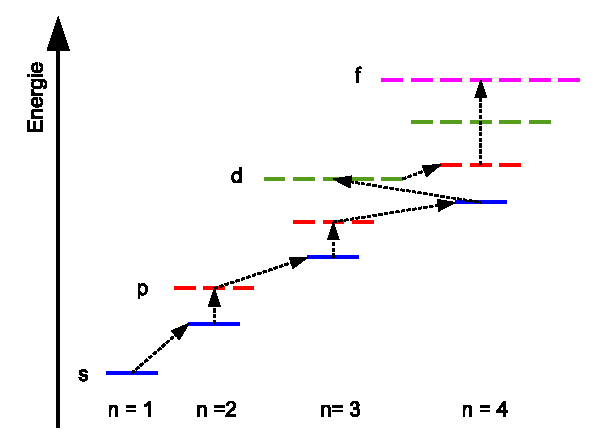
\includegraphics[scale=1]{VystavbovyPrincip.eps}
\caption[Výstavbový princip]{Pořadí orbitalů, které typicky nacházíme v~neutrálních atomech, se nazývá výstavbovým principem.}
\label{obr:Aufbau}
\end{figure}

\item \textbf{Pauliho vylučovací princip}. Zcela fundamentální princip, bez něj by periodická tabulka neexistovala, všechny prvky by v~základním stavu byly jenom různě vypasené atomy vodíku.

\item \textbf{Pravidlo maximální multiplicity}. O~Hundových pravidlech bude řečeno více dále.   
 
\end{itemize}

\noindent Z~Fockových rovnic také vyplývá tzv. Koopmansův teorém, dle kterého ionizační energie i-tého elektronu $IE_i$ rovna orbitální energii příslušného elektronu $\epsilon_i$ (až na znaménko) 

\begin{equation}
IE_i = - \varepsilon_i
\label{rov:VE-58}
\end{equation}

\noindent a orbitální energie nejnižšího neobsazeného elektronu (LUMO elektronu, z~angl. \textit{Lowest Unoccupied Molecular Orbital}) je zase rovna elektronové afinitě

\begin{equation}
EA = -\varepsilon_{\mathrm{LUMO}}.
\label{rov:VE-59}
\end{equation}

Pojďme se nyní podívat, jak se vyvíjí s~protonovým číslem kupříkladu ionizační energie nejvýše obsazeného elektronu (HOMO elektronu, z~angl. \textit{Highest Occupied Molecular Orbital}). Pro atom vodíkového typu by platilo

\begin{equation}
IE \sim \frac{(Z^{\prime})^2}{n^2}.
\label{rov:VE-60}
\end{equation}

\noindent Vnitřní elektrony ale velmi efektivně stíní náboj jádra, takže HOMO elektron cítí náboj zmenšený o~počet elektronů ve vnitřních slupkách. Jestliže se budeme pohybovat v~periodě od lithia k~neonu, očekávali bychom rostoucí ionizační energii: roste totiž protonové číslo a náboj jádra není ještě stíněn. Jestliže ale od neonu přejdeme k~sodíku, vzroste najednou skokově hlavní kvantové číslo $n$ a navíc efektivní protonové číslo se zmenší díky stínění náboje jádra vnitřními elektrony. Ionizační energie by se proto měla spíše blížit lithiu nežli neonu. To skutečně pozorujeme (pohleď, čtenáři, na obrázek~\ref{obr:Period}). Podobné úvahy vysvětlí i periodické změny poloměru atomů, který je pro jedno-elektronové atomy dán vztahem

\begin{equation}
R \sim \frac{n^2}{Z^{\prime}},
\label{rov:VE-61}
\end{equation}

\noindent či třeba periodicita elektronegativity, kterou můžeme dle Mullikena definovat jako

\begin{equation}
\chi = 0{,}187 (IE + EA) + 0{,}17.
\label{rov:VE-62}
\end{equation}

\begin{figure} [htb]
\centering
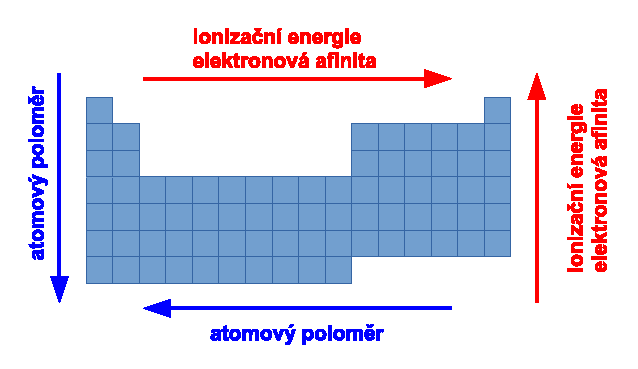
\includegraphics[scale=1]{PeriodicitaVlastnosti.eps}
\caption[Periodicita vlastností prvků]{Ionizační energie, elektronové afinity či poloměry atomů se s~protonovým číslem periodicky mění. Tato periodicita je důsledkem základních kvantově-mechanických zákonů.}
\label{obr:Period}
\end{figure}


\subsection{Sčítání momentu hybnosti a atomové termy}
Jedno-elektronové atomy jsou charakterizovány nejen energií, ale také hodnotou velikosti momentu hybnosti (kvantové číslo $l$) a projekcí momentu hybnosti do určité osy (konvenčně do osy z, kvantové číslo $m$). Jestliže studujeme atomy s~více elektrony, mohlo a mělo by nás zajímat, jakým způsobem se momenty hybností jednotlivých elektronů sčítají do celkového momentu hybnosti.

Celkový moment hybnosti $\vec{L}$ by měl splňovat kvantově-mechanická pravidla jako jakýkoliv jiný moment hybnosti. Pro jeho velikost tak bude platit

\begin{equation}
\vert \vec{L} \vert = \hbar \sqrt{L(L+1)}
\label{rov:VE-63}
\end{equation}

\noindent a pro projekci do směru osy $z$ pak

\begin{equation}
L_z = \hbar M.
\label{rov:VE-64}
\end{equation}
 

Uvažme případ dvou elektronů, z~nichž každý se nachází v~p orbitalu a je tedy charakterizován kvantovým číslem $l=1$.

\begin{eqnarray*}
l_1 &=& 1 \\
l_2 &=& 1
\end{eqnarray*}

\noindent Hodnota momentu hybnosti ve směru osy $z$ se pak může buďto sčítat a nebo odčítat. Udělejme si následující tabulku

\begin{table}[ht]
\centering
\begin{tabular}{c|ccc}
\toprule
    $_{m_1}\ddots^{m_2}$      & -1    & 0     & 1 \\
\midrule
    -1    & -2    & -1    & 0 \\
    0     & -1    & 0     & 1 \\
    1     & 0     & 1     & 2 \\
\bottomrule
\end{tabular}
\label{tab:ScitaniHybnosti}
\end{table}



Vidíme, že bude existovat stav, pro který kvantové číslo $M$ určující projekci celkového momentu hybnosti do osy $z$ nabývá hodnoty 2. Tomu ale odpovídá stav s~velikostí momentu hybnosti daného kvantovým číslem $L = 2$. K~tomuto kvantovému číslu ovšem přísluší ještě hodnoty $M=+1,0,-1,-2$. V~tabulce nám tedy zbývají hodnoty $M =-1,0,0,1$. Je zjevné, že tedy musí existovat i stav s~hodnotou $L=1$. Tomu odpovídají hodnoty $M=-1,0, 1$. Zbývá tedy ještě $M=0$, čemuž odpovídá $L=0$. Vidíme tedy, že ze dvou elektronů ve stavu $l=1$ můžeme dostat $L=2,1,0$. 

Tuto naši úvahu můžeme zobecnit. Máme-li dva elektrony ve stavu $l_1$ a $l_1$, pak celkový moment hybnosti může nabývat hodnot

\begin{equation}
L = \vert l_1 - l_2 \vert , \dots , l_1 + l_2.
\label{rov:VE-65}
\end{equation}

Stejným způsobem můžeme sčítat také celkový orbitální moment $\vec{L}$ a celkový spinový moment $\vec{S}$ do celkového momentu $\vec{J} = \vec{L} + \vec{S}$. Pro kvantové číslo $J$ bude platit

\begin{equation}
J = \vert L - S \vert, \dots, L+S.
\label{rov:VE-66}
\end{equation}


Stav atomu potom zapisujeme pomocí tzv. atomového termu


\begin{figure} [ht]
\centering
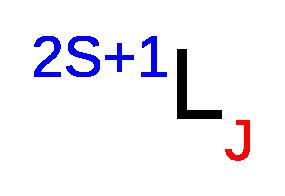
\includegraphics[scale=0.8]{AtomovyTerm.eps}
\caption[Atomové termy]{Symbol používaný pro vyjádření stavu mnoho-elektronového atomu}
\label{obr:ATerm}
\end{figure}

\begin{priklad}
\textbf{Zadání:} Při plamenných zkouškách je nejsnadnější poznat přítomnost sodíku díky vyzařování intenzivního žlutého světla. Toto světlo odpovídá přechodu nepárového elektronu z 2p orbitalu sodíku do orbitalu 2s. Už v 19. století se zjistilo, že jde o~dvě velmi blízko ležící čáry,  jedna u 589,0~nm a druhá u 589,6~nm. Jakým dvěma přechodům tyto emisní čáry odpovídají?\\[0.1cm]
\textbf{Řešení:} Sodík s nepárovým  elektronem v 2p orbitalu se může nacházet ve dvou stavech lišícím se kvantovým číslem J. Kvantové číslo $L=1$, kvantové číslo $S=1/2$, pak $J=|L-S|,\, L+S$ tedy dá $J=1/2,\,3/2$.

Půjde tedy o přechody ze stavů $^2$P$_{1/2}$ a $^2$P$_{3/2}$ do $^2$S$_0$ stavu, což je základní stav atomu sodíku. Dle Hundových pravidel bude energeticky níže stav $^2$P$_{1/2}$, tj. přechod u 589,6~nm odpovídá deexcitaci z tohoto stavu.
\end{priklad}

Musíme mít ovšem na paměti, že ne všechny součty jsou v~atomech možné (díky Pauliho vylučovacímu principu).



\subsubsection{Hundova pravidla}
Pořadí jednotlivých atomových termů dle energie je dáno tzv. Hundovými pravidly. Níže uvádíme jejich přehled.

\begin{itemize}
\item Term s~maximální multiplicitou má nejnižší energii.

\item Je-li multiplicita dvou termů stejná, pak nižší energii má term s~vyšší hodnotou $L$.

\item Je-li multiplicita i $L$ dvou termů stejná, pak pro slupky méně než z~poloviny zaplněné má nižší energii stav s~nižším $J$.  
 
\end{itemize}

\begin{priklad}
\textbf{Zadání:} S pomocí Hundových pravidel odvoďte základní stav atomu uhlíku a~zapište dovolené termy.\\[0.1cm]
\textbf{Řešení:} Základní elektronový stav má plnou elektronovou konfiguraci
\begin{displaymath}
1\mathrm{s}^2 \, 2\mathrm{s}^2 \, 2\mathrm{p}^2
\end{displaymath}
nebo ve zkrácené podobě
\begin{displaymath}
^{2} \mathrm{He}: 2\mathrm{s}^2 \, 2\mathrm{p}^2.
\end{displaymath}
Dále víme, že plně zaplněné slupky nemusíme uvažovat. Došli jsme tak k~závěru, že základní stav atomu uhlíku odpovídá elektronové konfiguraci 2p$^2$. Tomu odpovídají termy
\begin{displaymath}
^{1}\mathrm{S}_0, \, ^{3}\mathrm{P}_0, \, ^{3}\mathrm{P}_1, \, ^{3}\mathrm{P}_2 \mbox{ a } ^{1}\mathrm{D}_2.
\end{displaymath} \vspace{-0.7cm}
\end{priklad}


V~nerelativistické kvantové mechanice by se energie stavů lišících se pouze hodnotou celkového momentu hybnosti $J$ neměla lišit. Rozdíl energií je způsoben tzv. spin-orbitální vazbou. Zhruba řečeno, elektron rotující kolem jádra generuje magnetické pole. Spin elektronu je vůči tomuto poli různým způsobem orientován a tím je ovlivněna i jeho energie. V~hamiltoniánu tak přibývá člen

\begin{equation}
\hat{H}_{SO} = \xi \hat{L} \hat{S}.
\label{rov:VE-67}
\end{equation}

\noindent Parametr $\xi$ představuje pro lehká jádra jenom velmi malý člen, Ten však rychle roste a pro těžká jádra je třeba tento jev brát v~potaz. Sčítání momentů hybnosti se dá provádět dvojím způsobem

\begin{itemize}
\item \textbf{L-S vazba (Russelova-Saundersova)}. Zde nejdříve sčítáme orbitální moment hybnosti pro celý atom, zvláště spinový moment pro celý atom a teprve na konci sečteme oba momenty. Uplatňuje se v~situacích, kdy je mezi-elektronová repulze významnějším efektem v~porovnání se spin-orbitální vazbou.  

\item \textbf{j-j vazba}. Zde nejdříve sčítáme orbitální a spinový moment pro jednotlivé elektrony a~sčítáme teprve výsledný moment hybnosti. 

\end{itemize}     



   
    


   

 



 




 


\clearpage
\section{Kvantová teorie molekul}
\label{kap:molekuly}
Popis molekul v~rámci kvantové teorie je ústředním tématem kvantové chemie. Na rozdíl od atomů nejsou molekuly centrálně symetrické, což výpočty jejich vlastností komplikuje. V~důsledku nižší symetrie se tak například v~molekulách při elektronovém pohybu nezachovává moment hybnosti. V~případě molekul se musíme kromě pohybu elektronů vyrovnat také s~pohyby atomových jader. Atomová jádra jsou daleko těžší než elektrony, takže jejich popis na kvantové úrovni není vždy nezbytně nutný. Je ovšem třeba vědět, jaká jsou omezení klasického pohledu na atomová jádra. Díky rozdílné hmotnosti jader a elektronů můžeme pohyb atomových jader a elektronů (často) oddělit. To je podstatou tzv. Bornovy-Oppenheimerovy aproximace vedoucí ke konceptu hyperplochy potenciální energie. Tento koncept je pro chemika důležitý natolik, že si možná ani neuvědomí jeho přibližnou povahu.  


\subsection{Molekulový Hamiltonián}


Nemělo by nám již být zatěžko zapsat pro molekulu hamiltonián. Ten musí obsáhnout všechny molekulové interakce mezi jádry a elektrony. Při zanedbání relativistických efektů nabývá následující tvar:

\begin{equation}
\hat{H}=\hat{T}_R+\hat{T}_r+\hat{V}_{nn}+\hat{V}_{nr}+\hat{V}_{rr}, 
\label{rov:mol-Hamiltonian}
\end{equation}

\noindent kde $\hat{T}_R$ je operátor kinetická energie jader:

\begin{equation}
\hat{T}_R=\sum_i	-\frac{\hbar^2}{2m_{n,i}}\Delta_{i}, 	
\end{equation}

\noindent $\hat{T}_r$ operátor kinetická energie elektronů:

\begin{equation}
\hat{T}_r=\sum_j	-\frac{\hbar^2}{2m_{e}}\Delta_{j}, 	
\end{equation}

\noindent $\hat{V}_{nn}$ popisuje coulombovské odpuzování mezi jádry:

\begin{equation}
\hat{V}_{nn}=\frac{1}{4\pi\epsilon_0}\sum_i\sum_{i'>i}\frac{Z_iZ_{i'} e^2}{ \left\vert \textbf{R}_i - \textbf{R}_{i'}\right\vert } , 	
\end{equation}

\noindent $\hat{V}_{nr}$ popisuje přitahování mezi jádry a elektrony:
\begin{equation}
\hat{V}_{nr}=\frac{1}{4\pi\epsilon_0}\sum_i\sum_j\frac{Z_i e^2}{ \left\vert \textbf{R}_i - \textbf{r}_j\right\vert } , 	
\end{equation}

\noindent a $\hat{V}_{rr}$ popisuje odpuzování mezi elektrony:

\begin{equation}
\hat{V}_{rr}=\frac{1}{4\pi\epsilon_0}\sum_j\sum_{j'>j}\frac{ e^2}{ \left\vert \textbf{r}_j - \textbf{r}_{r'}\right\vert }. 	
\end{equation}

\noindent Ve výše uvedených výrazech jsou $\textbf{R}_i$ a $\textbf{r}_j$ symboly pro polohové vektory pro jádro $i$ a elektron $j$, $Z_i$ pak značí náboj jádra $i$. Naším úkolem je vyřešit Schrödingerovu rovnici

\begin{equation}
\hat{H}\psi=E\psi
\end{equation}

\noindent kde vlnová funkce $\psi$ je funkcí jak souřadnic elektronů, tak souřadnic atomových jader. 

\subsection{Bornova-Oppenheimerova aproximace}

Přesné řešení Schrödingerovy rovnice s~molekulovým hamiltoniánem je mimořádně komplikované. Situaci nám ale hodně zjednoduší oddělení pohybu elektronů a atomových jader v~rámci Bornovy-Oppenheimerovy aproximace (BOA). Nejprve se na BOA podíváme stručně s~nadhledem, poté již budeme matematicky rigoróznější. 

\subsubsection{Bornova-Oppenheimerova aproximace: První pohled}


I~nejlehčí atomové jádro (proton) je přibližně 1800krát těžší než elektron.  Pohybuje se proto také mnohem pomaleji než elektron. Kvantový elektron tak v~každé chvíli vidí v~podstatě stojící, klasická atomová jádra. Pro každou geometrii jader můžeme proto vyřešit elektronovou Schrödingerovu rovnici a vypočítat příslušnou energii, se kterou se elektrony v~molekule v~dané geometrii pohybují:

\begin{equation}
\hat{H}_{el}\psi_{el}=E_{el}\psi_{el},
\end{equation}

\noindent kde $\hat{H}_{el}$ je elektronový Hamiltonián:

\begin{equation}
\hat{H}_{el}=\hat{T}_r+\hat{V}_{nr}+\hat{V}_{rr}+\hat{V}_{nn}
\end{equation}

\noindent a $E_{el}$ je elektronová energie (energie, se kterou se v~molekule pohybují elektrony, tato energie v~sobě většinou zahrnuje i coulombovské odpuzování mezi atomovými jádry). $\psi_{el}$ je pak elektronová vlnová funkce. Ta je funkcí souřadnic elektronů $\textbf{r}_j$, parametricky je ale závislá i na souřadnicích atomových jader. Pojmem \uv{parametrická závislost} máme na mysli, že elektronová vlnová funkce bude jiná pro každou geometrii $\textbf{R}_i$ a pro každou geometrii spočítáme také jinou elektronovou energii $E_{el}$. 

Závislost elektronové energie na souřadnicích atomových jader se pro dvouatomové molekuly nazývá křivkou potenciální energie, pro víceatomové molekuly potom hyperplochou potenciální energie. Hyperplocha potenciální energie je ústřední pojem teoretické chemie, který dává chemikovi jasnou představu o~struktuře a reaktivitě molekul. 

\begin{figure} [ht]
\centering
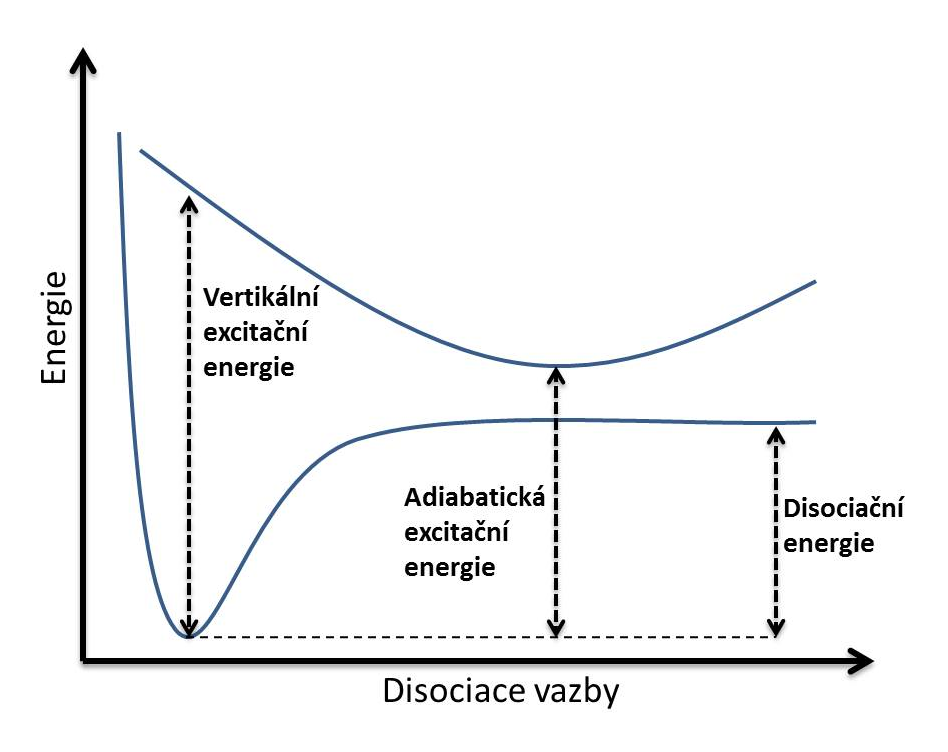
\includegraphics[scale=0.6]{obrazky/disociace2.eps}
\caption[disociace2]{Co lze vyčíst z~hyperplochy potenciální energie}
\label{obr:mol:disociace2}
\end{figure}

Obr. \ref{obr:mol:disociace2} znázorňuje křivku potenciální energie pro obecný případ dvouatomové molekuly. Křivky jsou vykresleny pro dva elektronové stavy. Na těchto křivkách jsou vyznačeny rovnovážné geometrie v~základním a v~excitovaném stavu a některé významné energetické údaje.


Hyperplochu potenciální energie si nyní ukážeme na několika konkrétních příkladech. Obr. \ref{obr:mol:H2_Ar} zobrazuje hyperplochy potenciálních energií pro $\mathrm{H}_2^+$ a dvouatomový komplex argonu. Hyperplocha (nebo v~tomto případě křivka) potenciální energie nám říká, jak na sebe působí atomy či molekuly. Podívejme se nejprve křivku potenciální energie $\mathrm{H}_2^+$. Modrá křivka zobrazující základní elektronový stav má minimum ve vzdálenosti kolem 0,1~nm. Tato vzdálenost odpovídá rovnovážné geometrii molekuly $\mathrm{H}_2^+$ . Červená křivka znázorňující elektronově excitovaný stav naopak žádné minimum nemá. Energie tohoto stavu je tím nižší, čím jsou atomy vodíku dál od sebe. Z~této křivky vidíme, že molekula $\mathrm{H}_2^+$ se v~excitovaném stavu rozpadne.

\begin{figure} [ht]
\centering
\begin{center}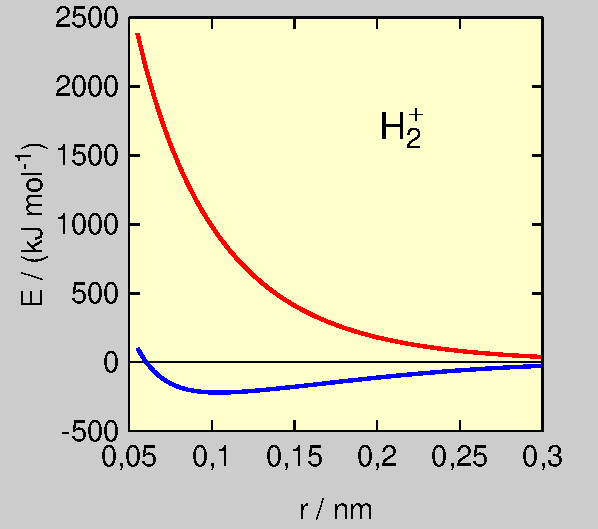
\includegraphics[scale=0.8]{obrazky/h2+.pdf}\hspace*{-1pt}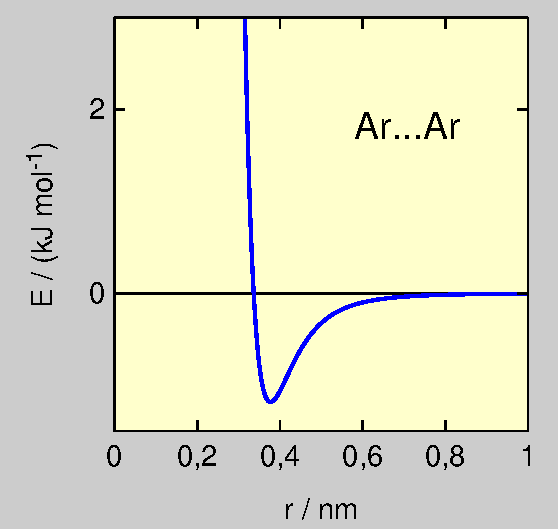
\includegraphics[scale=0.8]{obrazky/arar.pdf}\end{center}
\caption{Křivky potenciální energie pro $\mathrm{H}_2^+$ a dvouatomový komplex argonu. Energie v~obou případech byly vypočítány řešením stacionární Schrödingerovy rovnice.}
\label{obr:mol:H2_Ar}
\end{figure}

Druhý obrázek znázorňuje dva atomy argonu. Ze střední školy si všichni pamatujeme, že vzácné plyny netvoří dvouatomové molekuly. Křivka potenciální energie argonu nicméně vykazuje minimum. Nejde však o~chemickou vazbu. Všimněme si, že energetické minimum pro argon je mnohem dál než minimum pro $\mathrm{H}_2^+$. Navíc, podíváme-li se na energetickou osu, všimneme si, že minimum u~argonu není ani zdaleka tak hluboké jako bylo v~případě $\mathrm{H}_2^+$. Argon vskutku netvoří chemické vazby, ale je stabilizován pouze slabými nekovalentními interakcemi, konkrétně tzv. disperzními silami.


\begin{figure} [ht]
\centering
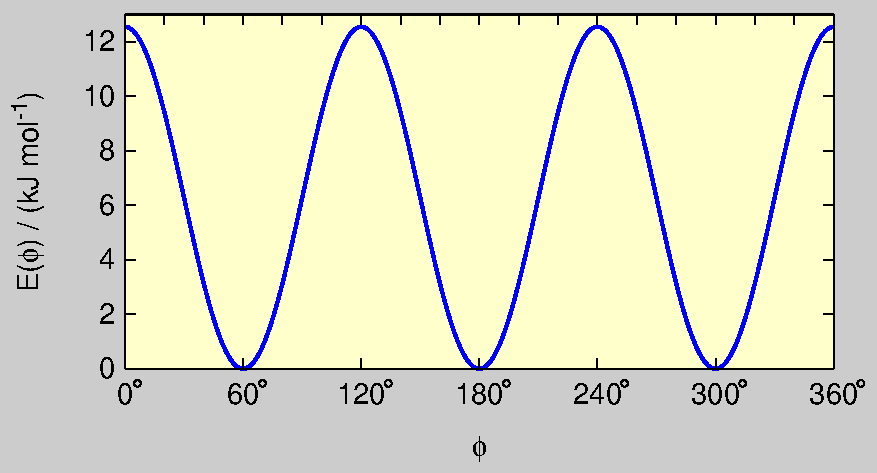
\includegraphics[scale=0.9]{obrazky/ethane.pdf}
\caption{Závislost potenciální energie na vzájemném otáčení methylových skupin v~molekule ethanu.}
\label{obr:mol:ethan}
\end{figure}

Další příklad si vypůjčíme ze základního kurzu organické chemie. Molekula ethanu obsahuje dvě methylové skupiny. Pokud jednu methylovou skupinu otočíme, bude se měnit potenciální energie (tj. elektronová energie) této molekuly. Dva limitní příklady nazýváme zákrytová a nezákrytová konformace. Obr. \ref{obr:mol:ethan} ukazuje energetiku otáčení methylové skupiny, přičemž všechny energie byly opět vypočítány řešením stacionární Schrödingerovy rovnice.

\begin{figure} [ht]
\centering
\begin{center}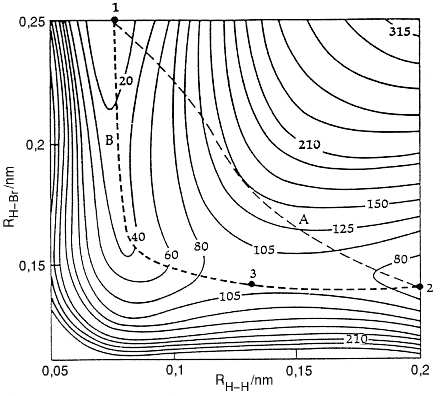
\includegraphics[scale=1.0]{obrazky/potsurface1.pdf}\hfill\raise 2mm\hbox{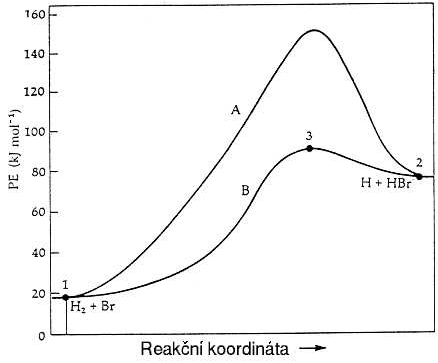
\includegraphics[scale=1.0]{obrazky/potsurface2.pdf}}
\end{center}
\caption{Vrstevnicový diagram potenciální energie pro reakci Br + HBr.}
\label{obr:mol:HBr}
\end{figure}

Poslední příklad nám ukáže, že pojem hyperplocha potenciální energie je důležitý také v~chemické kinetice. Podívejme se na vznik bromovodíku podle následující reakce:

\begin{equation}
\mathrm{H}_2+\mathrm{Br}\longrightarrow\mathrm{HBr}+\mathrm{H}, 
\end{equation} 

\noindent kde se přenese atom vodíku k~bromu, jedna chemická vazba zanikne a druhá vznikne. Elektronová energie systému o~třech atomech závisí na třech souřadnicích, což již ve dvou rozměrech neznázorníme. Vybereme si proto jenom dvě souřadnice, vzdálenost mezi dvěma atomy vodíku a vzdálenost mezi atomem vodíku a atomem bromu. Závislost energie na geometrii pak znázorníme pomocí vrstevnicového diagramu (viz obr. \ref{obr:mol:HBr}). Údaje ve vrstevnicovém diagramu odečítáme podobně jako v~mapě. Analogicky také hledáme nejméně náročnou cestu od reaktantů k~produktů, tj. údolím reaktantů přes sedlo k~údolí produktů (obrázek znázorňuje ještě jinou, energeticky náročnější konkurenční reakční cestu). Takovéto reakční cestě říkáme reakční koordináta. V~pravé části obrázku pak vidíme energetický profil reakce podél této reakční koordináty. 

Hyperplocha potenciální energie je smysluplný pojem pouze pokud je pohyb atomových jader a elektronů je nezávislý. Matematicky tuto nezávislost formulujeme tak, že celkovou vlnovou funkci zapíšeme jako součin vlnové funkce elektronů ($\psi_{el}$) a vlnové funkce jader ($\chi$)

\begin{equation}
\psi=\chi(\textbf{R})\psi_{el}(\textbf{r};\textbf{R}).
\label{rov:mol-BO}
\end{equation}


\subsubsection{Bornova-Oppenheimerova aproximace: Odvození}
Vyjdeme z~elektronového hamiltoniánu, který popisuje elektrony pro stojící jádra v~konkrétní geometrii $\textbf{R}_i$: 

\begin{displaymath}
\hat{H}_{el}=\hat{T}_r+\hat{V}_{nr}+\hat{V}_{rr}+\hat{V}_{nn}.
\end{displaymath}

\noindent Elektronový hamiltonián působí toliko na funkce souřadnic elektronů (přičemž ale tento elektronový hamiltonián je různý pro různé souřadnice jader $\textbf{R}_i$). Vyřešme nejdříve pro každou z~možných geometrií elektronovou Schrödingerovu rovnici :

\begin{equation}
\hat{H}_{el}\psi_{el}^{(i)}=E_{el}^{(i)}\psi_{el}^{(i)}.
\end{equation}

\noindent Znovu připomeňme, že řešením je vlnová funkce souřadnic elektronů parametricky závislá na souřadnicích jader

\begin{equation}
\psi_{el}^{(i)}=\psi_{el}^{(i)}(\textbf{r}; \textbf{R}).
\end{equation}

\noindent Pod pojmem \uv{parametrická závislost} máme na mysli, že vlnová funkce je různá pro různé souřadnice jader, přičemž ale čtverec vlnové funkce nemá význam hustoty pravděpodobnosti nalezení jader v~určité geometrii $\textbf{R}_i$. Sada vlastních funkcí elektronového hamiltoniánu vytváří úplný soubor funkcí a můžeme tedy každou funkci souřadnic elektronů rozvinout do báze vlastních funkcí elektronového hamiltoniánu. Můžeme to učinit i pro celkovou vlnovou funkci: 

\begin{equation}
\psi(\textbf{r},\textbf{R})=\sum_i \chi_i(\textbf{R})\psi_{el}^{(i)}(\textbf{r}; \textbf{R}),
\label{rov:mol-BO2}
\end{equation}

\noindent kde $\chi_i(\textbf{R})$ jsou rozvojové koeficienty, které závisí na poloze jader. Doposud jsme se nedopustili žádné aproximace. Dosadíme tedy vlnovou funkci $\psi(\textbf{r},\textbf{R})$ do Schrödingerovy rovnice $\hat{H}\psi=E\psi$, jejíž levou stranu si dále upravíme:

\begin{equation}
\hat{H}\psi=\sum_i (\hat{T}_R+\hat{H}_{el})\chi_i\psi_{el}^{(i)}=\sum_i \left[\hat{T}_R(\chi_i\psi_{el}^{(i)}) + \chi_iE_{el}^{(i)}\psi_{el}^{(i)}\right].
\label{rov:mol-mat2}
\end{equation}

\noindent Nyní si upravíme první člen pravé strany poslední rovnice. Výklad zjednodušíme tím, že budeme uvažovat operátor kinetické energie pouze v~jednom rozměru, tj. 

\begin{displaymath}
\hat{T}_R=\frac{-\hbar^2}{2m_R}\frac{\mathrm{d}^2}{\mathrm{d}R^2}.
\end{displaymath}

\noindent Nyní se zaměříme na působení operátoru kinetické energie jader:

\begin{equation}
\hat{T}_R\chi_i\psi_{el}^{(i)}=\frac{\hbar^2}{2m_R}\left(
\psi_{el}^{(i)}\frac{\mathrm{d}^2\chi_i}{\mathrm{d}R^2}
+2\frac{\mathrm{d}\chi_i}{\mathrm{d}R}\frac{\mathrm{d}\psi_{el}^{(i)}}{\mathrm{d}R}+\chi_i\frac{\mathrm{d}^2\psi_{el}^{(i)}}{\mathrm{d}R^2}
\right)
\label{rov:mol-BOmat}
\end{equation}

\noindent Na tomto místě se dopustíme aproximace: zanedbáme poslední dva členy z~rovnice \ref{rov:mol-BOmat}, tedy
 
\begin{equation}
\hat{T}_R\chi_i\psi_{el}^{(i)}\approx\frac{\hbar^2}{2m_R}
\psi_{el}^{(i)}\frac{\mathrm{d}^2\chi_i}{\mathrm{d}R^2}.
\end{equation}

\noindent Z~odvození Bornovy-Oppenheimerovy aproximace jasně vidíme, že obecně bude platit tím lépe, čím méně se bude elektronová vlnová funkce měnit s~geometrií. Můžeme hned nabýt podezření, že pro rychle se pohybující jádra by Bornova-Oppenheimerova aproximace nemusela fungovat úplně dobře.

Vraťme se ještě k~rovnici \ref{rov:mol-mat2}. Rovnici nejprve vynásobíme komplexně sdruženou elektronovou vlnovou funkcí $\psi_{el}^{j}$ a následně prointegrujeme přes souřadnice elektronů $r$:

\begin{equation}
\sum_i \left[\hat{T}_R(\chi_i\psi_{el}^{(i)}) + \chi_iE_{el}^{(i)}\psi_{el}^{(i)}\right]=E\sum_i \psi_{el}^{(i)}\chi_i \qquad \qquad /.\psi_{el}^{(j)*},/\int d\tau
\end{equation}


\noindent Schrödingerova rovnice (v~jedné dimenzi) nabude tvaru:
\begin{equation}
\sum_i \left[\hat{T}_R\chi_i\int\psi_{el}^{(j)*}\psi_{el}^{(i)}d\tau + \chi_iE_{el}^{(i)}\int\psi_{el}^{(j)*}\psi_{el}^{(i)}d\tau\right]=E\sum_i \int \psi_{el}^{(j)*}\psi_{el}^{(i)}\chi_id\tau. 
\end{equation}
Vzhledem k~tomu, že elektronové vlnové funkce jsou ortonormální, rovnice se zjednoduší na následující tvar:
\begin{equation}
\sum_i \left[\hat{T}_R\chi_i\delta_{ij} + \chi_iE_{el}^{(i)}\delta_{ij}\right]=E\sum_i \int \delta_{ij}\chi_i. 
\end{equation}
Kroneckerovo $\delta$ nám nakonec vybere pouze členy pro $i=j$:

\begin{equation}
\left(\hat{T}_R+E_{el}^{(j)}\right)\chi_j=E\chi_j
\label{rov:mol-jadschr}
\end{equation}

\noindent Rovnice \ref{rov:mol-jadschr} představuje Schrödingerovu rovnici pro jádra. Vidíme, že jádra se pohybují v~potenciálu daného elektronovou energií pro jednotlivé geometrie. 

\subsubsection{Meze platnosti Bornovy-Oppenheimerovy aproximace}

Není těžké naleznout příklady, kdy Bornova-Oppenheimerova aproximace selhává. Vezměme si molekulu chloridu sodného (viz obr. \ref{obr:mol:NaCl disociace}). NaCl je v~základním stavu vázána iontovou vazbu, minimum základního stavu si tedy můžeme přibližně popsat jako $\mathrm{Na}^{+}\mathrm{Cl}^{-}$. Když od sebe oddalujeme atomy chloru a sodíku, roste energie, až dojde k~rozpadu chemické vazby. Molekula se může rozpadnout dvěma způsoby, na $\mathrm{Na}^{+}$ a $\mathrm{Cl}^{-}$ nebo na $\mathrm{Na}$ a $\mathrm{Cl}$, přičemž jedna limita odpovídá základnímu a druhá excitovanému stavu. Nyní uvažujme, že molekulu chloridu sodného excitujeme. Kovalentně vázaný excitovaný stav v~geometrii globálního minima není stabilní a bude se proto rozpadat. Tento rozpad by se dle Bornovy-Oppenheimerovy aproximace měl odehrávat na jedné křivce potenciální energie a výsledkem by tak měly být ionty $\mathrm{Na}^{+}\mathrm{Cl}^{-}$. Ve skutečnosti vzniknou oba produkty, jak iontový, tak kovalentní. V~oblasti křížení stavů se totiž elektronová vlnová funkce s~mezijadernou vzdáleností dramaticky mění a druhý a třetí člen v~rovnici \ref{rov:mol-BOmat} proto není možno zanedbat. 


\begin{figure} [ht]
\centering
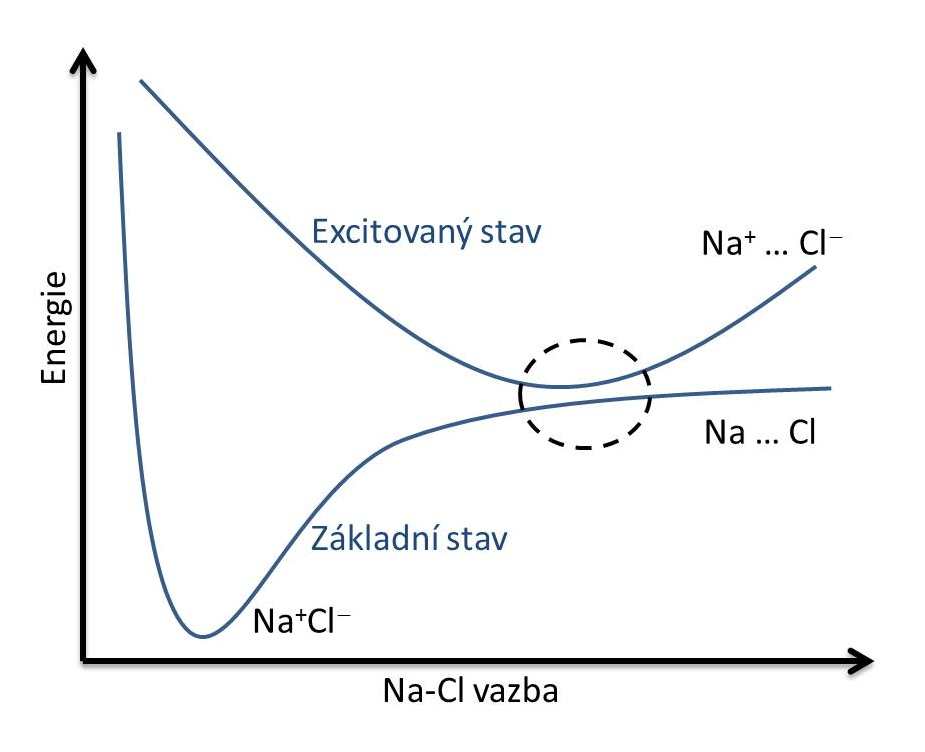
\includegraphics[scale=0.5]{obrazky/NaCl_disociace.eps}
\caption[NaCl disociace]{Ukázka selhání Bornovy-Oppenheimerovy aproximace}
\label{obr:mol:NaCl disociace}
\end{figure}


 


\clearpage
\section{Vibrace a rotace molekul}
\label{kap:vibrot}
Obecná molekula může konat translační, vibrační nebo rotační pohyby. V~této kapitole si ukážeme pouze nejjednodušší příklad, totiž popis vibrace a rotace dvouatomové molekuly.

\noindent V~minulé kapitole jsme si ukázali Schrödingerovu rovnici pro jádra (\ref{rov:mol-jadschr}):

\begin{displaymath}
\left(\hat{T}_R+E_{el}^{(j)}\right)\chi_j = E \chi_j.
\end{displaymath}

\noindent Pro zjednodušení budeme v~následujícím textu uvažovat platnost Bornovy-Oppenheimerovy aproximace a dále pouze základní elektronový stav molekuly:

\begin{displaymath}
\left(\hat{T}_R+E_{el}\right)\chi_j = E \chi_j.
\end{displaymath}
 
\noindent Jelikož uvažujeme dvouatomovou molekulu, bude elektronová energie $E_{el}$ pouze funkcí vzdálenosti dvou jader (označme je jako $\alpha$ a $\beta$)

\begin{displaymath}
E_{el}=E_{el}(\textbf{R}_{\alpha}-\textbf{R}_{\beta}),
\end{displaymath} 

\noindent ne na jejich orientaci.
Dalším krokem v~našem výkladu by bylo přeformulování kinetické energie na kinetickou energii těžiště molekuly a kinetickou energii odpovídající relativnímu pohybu molekuly. Celý postup je popsán v~kapitole o~problému dvou částic. Zde si uvedeme pouze dvě konečné rovncice, ke kterým bychom se dostali:

\begin{eqnarray}
\hat{H}_{tr}\psi_{tr}(R)=E_{tr}\psi_{tr}(R)
\label{vibrot:trans}\\
\hat{H}_{int}\psi_{int}(r)=E_{int}\psi_{tr}(r)
\label{vibrot:vibrot}\\
E=E_{tr}+E_{int},
\end{eqnarray}

\noindent přičemž první rovnice (\ref{vibrot:trans}) popisuje translaci molekuly jako celku a druhá (\ref{vibrot:vibrot}) její relativní pohyb, tedy vibraci nebo rotaci. Translaci jsme se  věnovali v~kapitole XX, nyní se v~dalším výkladu budeme věnovat vibracím a rotacím. Rovnici \ref{vibrot:vibrot} představující vnitřní problém si můžeme rozepsat následovně:

\begin{equation}
\left[-\frac{\hbar^2}{2\mu}\Delta_{\textbf{r}}+E_{el}(r)\right]\psi_{int}=E_{int}\psi_{int}
\label{vibrot:vibrot2}
\end{equation}


Tato rovnice představuje molekulu v~centrálním potenciálu. Také centrálnímu potenciálu jsme se věnovali v~kapitole s~problémem dvou částic. Ukázali jsme si, že řešení hledáme ve tvaru součinu sférické harmonické funkce a radiální vlnové funkce

\begin{equation}
\psi_{int}(r,\theta,\psi)=R(r)Y^m_l(\theta,\psi).
\end{equation}

\noindent Takovouto vlnovou funkci můžeme dosadit do Schr\"odingerovy rovnice a posléze vydělit sférickým harmonikem, abychom dostali radiální Schr\"odingerovu rovnici:

\begin{equation}
-\frac{\hbar^2}{2\mu}\left(R''+\frac{2}{r}R'\right)+\frac{l\left(l+1\right)\hbar^2}{2\mu r^2}R+\hat{V}R=E_{int}R,
\end{equation}

\noindent kterou si dále zjednodušíme zavedením substituce
\begin{displaymath}
F(r)=rR(r)
\end{displaymath}

\noindent na

\begin{equation}
-\frac{\hbar^2}{2\mu}F''+\left[E_{el}+\frac{l\left(l+1\right)\hbar^2}{2\mu r^2}\right]F=E_{int}F.
\label{vibrot:vibrot3}
\end{equation}

\noindent Poslední rovnici je možné zjednodušit, zavedeme-li si dvě aproximace. 

\begin{itemize}

\item Nejprve použijeme Taylorův rozvoj do druhého řádu pro vyjádření elektronové energie:

\begin{equation}
E_{el}\approx E_{el}(R_{ekv})+\left(\frac{dE_{el}}{dr}\right)(r-R_{ekv})+\frac{1}{2}\left(\frac{d^2E_{el}}{dr^2}\right)(r-R_{ekv})^2, 
\end{equation}

\noindent kde první člen určuje pouze relativní hladinu energie, a proto si můžeme zvolit $E_{el}(R_{ekv})=0$. Druhý člen je nulový, protože se nacházíme v~minimu a teprve třetí člen bude nenulový. Zavedeme-li si substituci

\begin{eqnarray}
k=\left(\frac{d^2E_{el}}{dr^2}\right)\nonumber \\
x=r-R_{ekv}\nonumber,
\end{eqnarray}

\noindent můžeme Taylorův rozvoj energie přepsat na následující tvar:

\begin{equation}
E_{el}\approx\frac{1}{2}\left(\frac{d^2E_{el}}{dr^2}\right)(r-R_{ekv})^2=\frac{1}{2}kx^2.
\end{equation}

\item Dále bychom si udělali Taylorův rozvoj ještě pro druhý člen v~závorce rovnice \ref{vibrot:vibrot3}:

\begin{equation}
\left(\frac{l\left(l+1\right)\hbar^2}{2\mu}\right)\frac{1}{r^2} =
\left(\frac{l\left(l+1\right)\hbar^2}{2\mu}\right)
\left[\frac{1}{R_{ekv}^2}
-\frac{2}{R_{ekv}^3}(r-R_{ekv})
+\frac{3}{R_{ekv}^4}(r-R_{ekv})^2+...
\right],
\end{equation}
ze kterého budeme v~tomto případě uvažovat pouze nultý člen:
\begin{equation}
\left(\frac{l\left(l+1\right)\hbar^2}{2\mu}\right)\frac{1}{r^2} \approx \left(\frac{l\left(l+1\right)\hbar^2}{2\mu}\right)\frac{1}{R_{ekv}^2}
\end{equation}
\end{itemize}

Uvažujeme-li tyto dvě aproximace, rovnice \ref{vibrot:vibrot3} přejde na 

\begin{equation}
-\frac{\hbar^2}{2\mu}F''+\left[\frac{1}{2}kx^2+\frac{l\left(l+1\right)\hbar^2}{2\mu R_{ekv}^2}\right]F=E_{int}F 
\label{vibrot:vibrot4}
\end{equation}

\noindent a po změně pořadí členů na 

\begin{equation}
-\frac{\hbar^2}{2\mu}F''+\frac{1}{2}kx^2F=\left(E_{int}-\frac{l\left(l+1\right)\hbar^2}{2\mu R_{ekv}^2}\right)F. 
\label{vibrot:vibrot5}
\end{equation}

\noindent Poslední rovnice je rovnicí pro jednodimenzionální harmonický oscilátor. Přepišme si ji ještě zavedením

\begin{displaymath}
E'=E_{int}-\frac{l\left(l+1\right)\hbar^2}{2\mu R_{ekv}^2}
\end{displaymath}

\noindent na

\begin{equation}
-\frac{\hbar^2}{2\mu}F''+\frac{1}{2}kx^2F=E'F. 
\label{vibrot:vibrot6}
\end{equation}

Protože víme, jak vypadá energie harmonického oscilátoru, můžeme dále psát

\begin{equation}
E'=\left(n+\frac{1}{2}\right)h\nu,
\end{equation}

\noindent kde $\nu=\frac{1}{2\pi}\sqrt[]{\frac{k}{\mu}}$. Při uvažování těchto vztahů dostaneme konečný vztah pro vnitřní energii, tedy

\begin{equation}
E_{int}\approx \left(n+\frac{1}{2}\right) h\nu+\frac{\hbar^2l(l+1)}{2\mu R_{ekv}^2}.
\end{equation}

\noindent Dva členy v~poslední rovnici zastupují harmonický oscilátor (vibrace) a tuhý rotor (rotace). 

\noindent V~průběhu odvození jsme použili aproximací harmonického oscilátoru a tuhého rotoru. Obě aproximace mají své limity. Harmonický oscilátor např. předpokládá, že vibrační hladiny jsou ekvidistantní a nedokáže také popsat disociaci vazby. Místo harmonického oscilátoru je možné použít oscilátoru Morseova

\begin{equation}
E_{el}=D_e\left[1-e^{a(r-R_{ekv})}\right],
\end{equation}

\noindent který už pracuje s~disociací vazby (disociační energie je $D_e$ a $a$ parametr vztahující se k~šířce potenciálu, $a=\sqrt[]{\frac{k}{2D_e}}$).
\noindent Pokud bychom chtěli vibrace a rotace popsat ještě přesněji, bylo by třeba uvažovat Coriolisovy interakce, tedy skutečnost, že vibrační a rotační pohyb není nezávislý.











\clearpage
\section{Elektronová struktura molekul}
\label{kap:elstruktmol}
\newcommand{\orbital}[3]{#1 \mathrm{#2}_{#3}}

Ústředním úkolem kvantové chemie po zavedení Bornovy-Oppenheimerovy aproximace je výpočet elektronové energie molekul

\begin{equation}
\hat{H}_e \psi_e (\vec{r}, \vec{R}) = E_e (\vec{R}) \psi_e(\vec{r}, \vec{R}),
\label{rov:ElStrukt-1}
\end{equation}

\noindent kde elektronová energie závisí na konkrétní geometrii molekuly, tj. na souřadnicích atomových jader $\vec{R}$. V~této kapitole probereme řešení rovnice \eqref{rov:ElStrukt-1} pro dvouatomové molekuly. Začneme přitom nejjednodušší molekulou, totiž iontem molekuly vodíku H$_2^+$.   

\subsection{Ion molekuly vodíku}

\begin{figure} [htb]
\centering
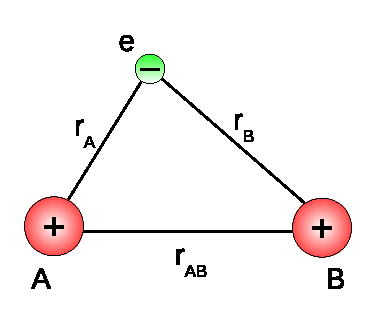
\includegraphics[scale=1]{IonVodiku.eps}
\caption[Ion H$_2^{+}$]{Geometrie iontu molekuly vodíku.}
\label{obr:IonVodiku}
\end{figure}

Ion molekuly vodíku je tvořen dvěma jádry (konkrétně protony), označme si je jako jádra A a~B, a jedním elektronem, viz obrázek~\ref{obr:IonVodiku}. Pro takovýto útvar nám není zatěžko napsat elektronový hamiltonián

\begin{equation}
\hat{H}_e = -\frac{\hbar^2}{2 m_e} \Delta_e - \frac{e^2}{4 \pi \epsilon_0} \left( \frac{1}{r_A} + \frac{1}{r_B} \right),
\label{rov:ElStrukt-2}
\end{equation}


\noindent kde
\begin{equation}
\Delta_e \equiv \frac{\partial^2}{\partial x_e^2} + \frac{\partial^2}{\partial y_e^2} + \frac{\partial^2}{\partial z_e^2}
\nonumber
\end{equation}
je Laplaceův operátor v~souřadnicích elektronu $x_e, y_e, z_e$. $r_A$ je souřadnice elektronu k~jádru A a~$r_B$ je souřadnice elektronu k~jádru B.\footnote{V elektronovém hamiltoniánu může, ale nemusí být přidán člen popisující coulombovské odpuzování mezi jádry $\frac{1}{4 \pi \epsilon_0} \frac{e^2}{r_{AB}}$. Z~pohledu elektronové vlnové funkce totiž tento člen představuje konstantu. Zde mezijadernou repulzi vynecháváme.}  Nadále bude poněkud pohodlnější pracovat v~soustavě atomových jednotek, ve kterých $\hbar = m_e=e=4\pi \epsilon = 1$. Hamiltonián pak nabude tvaru

\begin{equation}
\hat{H}_e = -\frac{1}{2}\Delta_e - \left( \frac{1}{r_A} + \frac{1}{r_B} \right).
\label{rov:ElStrukt-3}
\end{equation}

Elektronovou Schr\"odingerovu rovnici s~tímto hamiltoniánem je možné řešit analyticky. Nás ale bude zajímat řešení přibližné, tedy takové, které budeme moci využít i pro složitější molekuly. Můžeme se docela dobře odrazit z~naší znalosti elektronové struktury atomů. Kdybychom měli v~blízkosti elektronu pouze jádro A, pak bychom řešení znali: vlnová funkce by byla dána atomovým orbitalem vodíku $1s_A$. Stejně tak kdyby se elektron pohyboval v~blízkosti jádra B a~jádro A~se v~okolí vůbec nevyskytovalo, pak by exaktním řešením byl orbital $1s_B$. Připomeňme, že atomové orbitaly $1s_A$ a~$1s_B$ jsou matematickými funkcemi souřadnic elektronů, konkrétně

\begin{eqnarray}
1\mathrm{s}_A \equiv k^{3/2} \pi^{-1/2} e^{-k r_A}, \nonumber \\
1\mathrm{s}_B \equiv k^{3/2} \pi^{-1/2} e^{-k r_B}, 
\label{rov:ElStrukt-4}
\end{eqnarray}

\noindent kde pro jádro vodíku o~nábojovém čísle $Z=1$ je $k=1$ (pro elektron v~poli jádra He$^+$ je pak $k=2$ atd.). Pokud jsou obě jádra hodně daleko od sebe, pak přesné řešení je dáno jako

\begin{equation}
\varphi = c_A 1 \mathrm{s}_A + c_B 1\mathrm{s}_B.
\label{rov:ElStrukt-5}
\end{equation}

Uvažme situaci, kdy se elektron nachází v~blízkosti jádra A. Hodnota vlnové funkce $1s_B$ pak pro velké vzdálenosti $r_{AB}$ bude zanedbatelná a tento elektron je pak v~zásadě popsán orbitalem $1s_A$, chová se tedy jako elektron atomu A. Nebo se elektron nachází v~blízkosti jádra B a pak se chová jako elektron atomu B. My budeme předpokládat, že tuto formu vlnové funkce můžeme použít pro všechny mezi-jaderné vzdálenosti. Výraz \eqref{rov:ElStrukt-5} představuje zkusmou vlnovou funkci ve smyslu variačního principu: tato funkce je závislá na rozvojových koeficientech $c_A$ a $c_B$, které musíme určit minimalizací funkcionálu energie.\footnote{Jako variační parametr můžeme použít také parametr $k$. Ten je spojen s~nábojovým číslem. Je jasné, že pro disociovanou strukturu s~velkou mezijadernou vzdáleností $r_{AB}$ bude optimální hodnota $k=1$, budeme skutečně popisovat dva atomy vodíku. Pokud ale obě jádra přiblížíme na velmi malou vzdálenost, vlnová funkce se bude blížit orbitalu $1s$ iontu atomu helia a tedy $k=2$.} Tento tvar vlnové funkce je zárodkem metody označované zkratkou MO-LCAO (z~angl. \textit{Molecular Orbitals - Linear Combination of Atomic Orbitals}). Hledáme totiž vlnovou funkci jednoho elektronu pohybujícího se v~molekule (tedy hledáme tzv. molekulový orbital) ve formě lineární kombinace atomových orbitalů. To je klasický příklad lineárního funkcionálu, který vede k~sekulárním rovnicím, se kterými jsme se již několikráte setkali

\begin{eqnarray}
c_A (H_{AA} - E S_{AA}) + c_B (H_{AB} - E S_{AB}) = 0, \nonumber \\
c_A (H_{BA} - E S_{AB}) + c_B (H_{BB} - E S_{BB}) = 0,
\label{rov:ElStrukt-6}
\end{eqnarray}

\noindent kde coulombovský integrál $H_{AA}$ a $H_{BB}$, rezonanční integrál $H_{AB}$ a překryvový integrál $S_{AB}$ mají v~našem případě tvar

\begin{eqnarray}
H_{AA} = H_{BB} &=& \frac{1}{2} k^2 - k~- \frac{1}{r_{AB}} - e^{2 k~r_{AB}} \left( k~+ \frac{1}{r_{AB}} \right), \nonumber \\
H_{AB} &=& -\frac{1}{2}k S_{AB} - k~(2-k) (1+ k~r_{AB}) e^{-k r_{AB}}, \nonumber \\
S_{AB} &=& e^{-k r_{AB}} \left(1 + k~r_{AB} + \frac{1}{3}k^2 r_{AB}^2 \right).
\label{rov:ElStrukt-7}
\end{eqnarray}

Podmínkou netriviálního řešení sekulárních rovnic je nulovost sekulárního determinantu


\begin{equation}
\begin{vmatrix}
H_{AA} - E S_{AA} & H_{AB} - E S_{AB}\\
H_{BA} - E S_{AB} & H_{BB} - E S_{AB}
\end{vmatrix}
=0,
\label{rov:ElStrukt-8}
\end{equation}

\noindent což vede ke~dvěma možným hodnotám energie (uvažme přitom, že hodnota rezonančního integrálu $H_{AB}$ je záporná)

\begin{eqnarray}
E_1 = \frac{H_{AA} + H_{AB}}{1+S_{AB}}, \nonumber \\
E_2 = \frac{H_{AA} - H_{AB}}{1-S_{AB}}.
\label{rov:ElStrukt-9}
\end{eqnarray}

Jestliže dosadíme energii $E_1$ zpět do sekulárních rovnic (detaily viz příklad \ref{priklad var princip} v kapitole~\ref{kap:Lin Var funkcional}), získáme vztah 

\begin{equation}
c_A = c_B.
\label{rov:ElStrukt-10}
\end{equation}

Pokud do sekulárních rovnic  dosadíme za energii hodnotu $E_2$, získáme vztah

\begin{equation}
c_A = - c_B.
\label{rov:ElStrukt-11}
\end{equation}

\noindent Hodnoty rozvojových koeficientů se tak v~absolutní hodnotě musí rovnat, lišit se může pouze jejich znaménko. To jsme ani nemuseli počítat z~variačního principu, neboť to plyne přímo ze symetrie problému. Máme tak dvojí řešení. Pro základní stav s~energií $E_1$ je řešením molekulový orbital jako součet atomových orbitalů

\begin{equation}
\varphi_1 = c_A (1\mathrm{s}_A + 1\mathrm{s}_B).
\label{rov:ElStrukt-12}
\end{equation}

\noindent Mluvíme o~tzv. vazebném orbitalu. Pro excitovaný stav s~energií $E_2$ je řešením Schr\"odingerovy rovnice rozdíl těchto atomových orbitalů

\begin{equation}
\varphi_2 = c_A(1\mathrm{s}_A - 1\mathrm{s}_B).
\label{rov:ElStrukt-13}
\end{equation}

\noindent Zde mluvíme o~antivazebném orbitalu. Obrázek \ref{obr:Vodik-orbitaly} vysvětluje toto označení. Ve vazebném orbitalu je maximum elektronové hustoty soustředěno do oblasti mezi atomovými jádry. Takovéto uspořádání podporuje přibližování atomových jader. Na druhou stranu v~antivazebném orbitalu elektrony mezi jádry příliš nejsou a obě jádra se tak od sebe odpuzují.\footnote{Obrázek by mohl vzbuzovat dojem, že primární hnací silou chemické vazby je elektrostatické stínění odpudivé interakce mezi jádry. To je ale přinejmenším nepřesné. Hlavním tahounem poklesu energie při vzniku vazby je pokles kinetické energie elektronů.} 

\begin{figure} [htb]
\centering
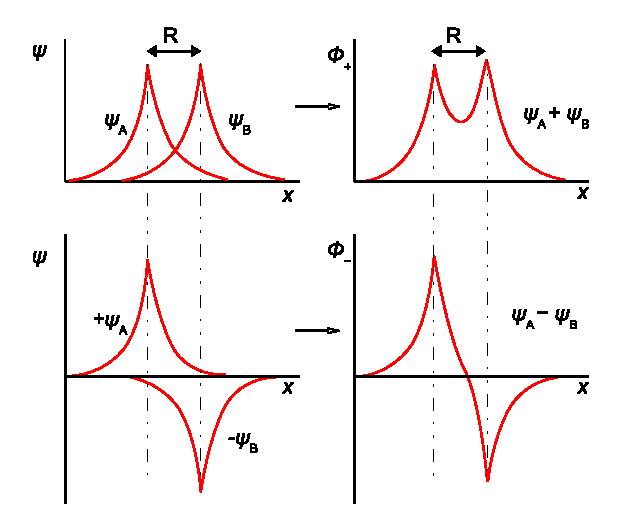
\includegraphics[scale=1]{Orbitaly.eps}
\caption[Orbitaly iontu vodíku]{Vazebný a antivazebný orbital iontu molekuly vodíku.}
\label{obr:Vodik-orbitaly}
\end{figure}

\begin{figure} [htb]
\centering
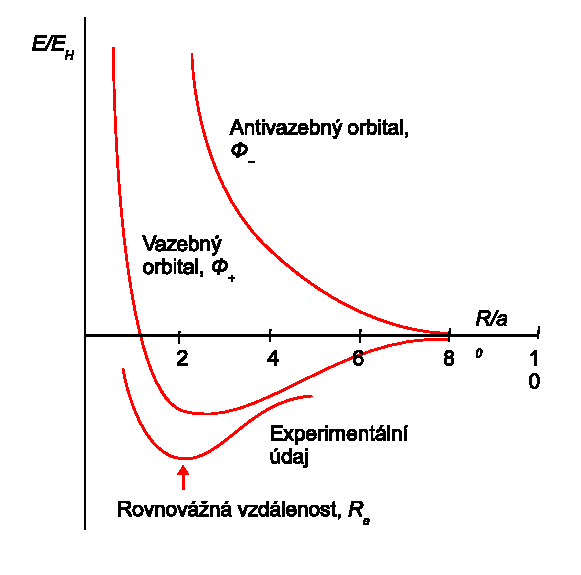
\includegraphics[scale=1]{PotencialovaKrivka.eps}
\caption[Potenciálové křivky iontu vodíku]{Potenciálové křivky dvou nejnižších stavů iontu molekuly vodíku.}
\label{obr:PotencialovaKrivka}
\end{figure}

\noindent Z~rovnice \eqref{rov:ElStrukt-7} můžeme do grafu snadno vynést energie $E_1$ a $E_2$ v~závislosti na mezijaderné vzdálenosti $r_{AB}$. Přidáme-li ještě mezijadernou repulzi $1/r_{AB}$, získáme křivky zobrazené na obrázku~\ref{obr:PotencialovaKrivka}.

Pro úplnost zbývá ještě doplnit, že konkrétní hodnotu rozvojového koeficientu $c_A$ získáme z~normalizačních podmínek


\begin{eqnarray}
1 &=& \int \vert \varphi_1 \vert^2 \mathrm{d}\tau = c_A^2 \int (1\mathrm{s}_A^2 + 1 \mathrm{s}_B^2 + 2 \cdot 1\mathrm{s}_A 1\mathrm{s}_B) \mathrm{d}\tau = c_A^2 (2 + 2S_{AB}), \nonumber \\
1 &=& \int \vert \varphi_2 \vert^2 \mathrm{d}\tau = c_A^2 \int (1\mathrm{s}_A^2 + 1 \mathrm{s}_B^2 - 2 \cdot 1\mathrm{s}_A 1\mathrm{s}_B) \mathrm{d}\tau = c_A^2 (2 - 2S_{AB}), 
\label{rov:ElStrukt-14}
\end{eqnarray}


\noindent a vlnová funkce tak má tvar


\begin{eqnarray}
\phi_1 &=& \frac{1\mathrm{s}_A + 1\mathrm{s}_B}{\sqrt{2}(1+S_{AB})}, \nonumber \\
\phi_2 &=& \frac{1\mathrm{s}_A - 1\mathrm{s}_B}{\sqrt{2}(1-S_{AB})}.
\label{rov:ElStrukt-15}
\end{eqnarray}

\subsection{Molekulové orbitaly excitovaných stavů}

Výpočet elektronové energie iontu molekuly vodíku představený v~minulé kapitole je pouze velmi přibližný. Jak bychom jej mohli vylepšit? Jednou z~možností by bylo považovat $k$ v~\eqref{rov:ElStrukt-4} za variační parametr. To je ale matematicky poněkud obtížnější úkol, neměli bychom pak již lineární funkcionál. Jinou, fyzikálně dobře motivovanou, možností je rozvinout molekulové orbitaly do rozsáhlejší množiny atomových orbitalů, například uvažovat elektron pohybující se ne pouze v~základním stavu atomu vodíku, ale i v~jeho stavech excitovaných. Mohli bychom například psát

\begin{eqnarray}
\varphi &=& c_1 \orbital{1}{s}{A} + c_2 \orbital{1}{s}{B} + c_3 \orbital{2}{s}{A} + c_4 \orbital{2}{s}{B} + \nonumber \\
&+& c_5 \orbital{2}{(p_1)}{A} + c_6 \orbital{2}{(p_1)}{B} + c_7 \orbital{2}{(p_0)}{A} + c_8 \orbital{2}{(p_0)}{B} + c_9 \orbital{2}{(p_{-1})}{A} + c_{10} \orbital{2}{(p_{-1})}{B}.
\label{rov:ElStrukt-16}
\end{eqnarray}

\noindent Takovýto rozvoj zvýší flexibilitu vlnové funkce. Sekulární rovnice nyní již představují soustavu deseti rovnic pro deset neznámých rozvojových koeficientů. Pořád ale jde o~soustavu lineárních rovnic, které jsou snadno řešitelné. Na místo dvou stavů ale nyní získáme stavů deset. V~základním stavu získáme řešením funkci, jejímž dominantním členem bude součet $1s_A+1s_B$, ale v~určité malé míře budou k~řešení přispívat i orbitaly $2s_A$, $(2p_0)_A$, $2s_B$ či $(2p_0)_A$. V~excitovaných stavech se začnou výrazněji uplatňovat i vyšší atomové orbitaly. Při kombinování atomových orbitalů do orbitalů molekulových bude platit:

\begin{itemize}
\item V~jednom molekulovém orbitalu se budou výrazněji uplatňovat pouze atomové orbitaly o~podobné energii. To vyplývá jednak z~matematiky celého problému, jednak i ze selského rozumu. Jestliže se elektron v~atomu A~pohybuje s~určitou energií, nemůžeme asi čekat, že se v~blízkosti atomu B jeho energie závratně změní.

\item Kombinují se toliko atomové orbitaly o~stejné symetrii vůči prvkům symetrie dané molekuly. Nebude se tak kombinovat orbital $1s_A$ s~orbitalem $(2p_1)_B$, neboť tyto orbitaly mají nulový překryv. Díky tomu můžeme řešit zvlášť sekulární problém pro $\sigma$ a $\pi$ elektrony

\begin{eqnarray}
\varphi_{\sigma} &=& c_1 \orbital{1}{s}{A} + c_2 \orbital{1}{s}{B} + c_3 \orbital{
2}{s}{A} + c_4 \orbital{2}{s}{B} + c_5 \orbital{2}{(p_0)}{A} + c_6 \orbital{2}{(p_0)}{B}, \nonumber \\
\varphi_{\pi} &=& c_1 \orbital{2}{(p_1)}{A} + c_2 \orbital{2}{(p_1)}{B} + c_3 \orbital{
2}{(p_{-1})}{A} + c_4 \orbital{2}{(p_{-1})}{B}.
\label{rov:ElStrukt-17}
\end{eqnarray}

\end{itemize}


\subsection{Více-elektronové molekuly}
Není asi snadné nadchnout chemika pro otázky spojené s~iontem molekuly vodíku. Skutečně, skoro vše, co chemika zajímá, má elektronů více. Mohou nám nějak výše uvedené úvahy pomoci při řešení otázek spojenými s~více-elektronovými molekulami? Ano, mohou. V~rámci Hartreeho-Fockovy aproximace totiž $N$-elektronovou Schr\"odingerovu rovnici 

\begin{equation}
\hat{H} \psi (\vec{r_1}, \vec{r_2}, \dots \vec{r_N}) = E_e\psi (\vec{r_1}, \vec{r_2}, \dots \vec{r_N})
\label{rov:ElStrukt-18}
\end{equation}

\noindent redukujeme na $N$ jedno-elektronových Fockových rovnic pro jednotlivé elektrony

\begin{equation}
\hat{F}_i \phi_i (\vec{r_i}) = \varepsilon_i \phi_i (\vec{r_i}).
\label{rov:ElStrukt-19}
\end{equation}

\noindent Fockovy rovnice obsahují složitější operátor než ten, se kterým jsme se setkali při řešení iontu molekuly vodíku, vše co bylo řečeno ale platí i pro molekulové orbitaly více-elektronových molekul. Stále tak hledáme molekulové orbitaly $\phi$ jako lineární kombinace atomových orbitalů $\chi_j$

\begin{equation}
\varphi_i(\vec{r_i}) = \sum_i c_{ji} \chi_j (\vec{r_i}),
\label{rov:ElStrukt-20}
\end{equation}

\noindent přičemž rozvojové koeficienty $c_{ji}$ získáváme pomocí variačního principu. Výsledky takovýchto výpočtů jsou důvěrně známé každému pečlivějšímu čtenáři základních učebnic anorganické chemie. Uplatňují se přitom dvě výše zmíněná pravidla o~kombinování orbitalů. Není cílem této přednášky dopodrobna opakovat celý tak důvěrně známý příběh. Pro připomenutí však čtenáře odkazujeme na obrázek~\ref{obr:Diatomy} zobrazující elektronové hladiny v~homonuklárních diatomických molekulách.

\begin{figure} [htb]
\centering
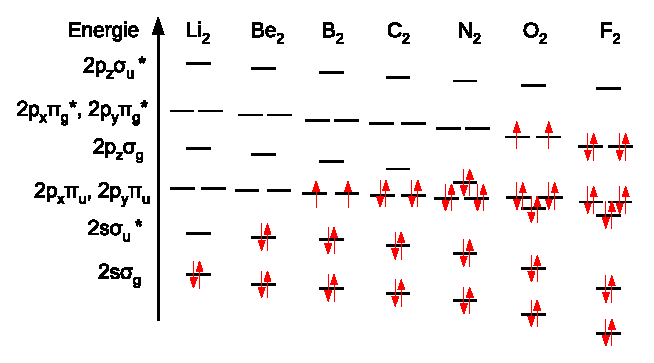
\includegraphics[scale=1]{Diatomy.eps}
\caption[Diatomické molekuly]{Jednoelektronové stavy v homonukleárních diatomických molekulách.}
\label{obr:Diatomy}
\end{figure}

Připomeňme také, že s~výše uvedenými orbitálními diagramy je spojen pojem řád vazby, definovaný jako

\begin{equation}
BO = \frac{n_r - n^{\ast}}{2}
\label{rov:ElStrukt-21}
\end{equation}

\noindent který nám říká, \uv{kolikatinásobná} je příslušná vazba. Číslo $n_r$ je počet elektronů ve vazebných orbitalech a $n^{\ast}$ je počet elektronů v~antivazebných orbitalech. Tak například vidíme, že molekula dusíku je vázána trojnásobnou vazbou. Taktéž by nám neměla uniknout překvapivá prediktivní síla kvalitativní teorie molekulových orbitalů. Z~diagramu pro molekulu O$_2$ kupříkladu hned vidíme, že tato molekula by měla být paramagnetická, neboť představuje dle Hundova pravidla biradikál, má totiž dva nepárové elektrony.

Zatím jsme se dívali pouze na diatomické molekuly tvořené dvěma stejnými atomy (homonukleární diatomika. Nic nám ale nebrání hledat molekulové orbitaly popisující pohyb elektronů v~diatomických molekulách s~nestejnými atomy. Podívejme se na případ molekuly NO. Energie 2p orbitalu atomu dusíku je -15~eV, energie 2p orbitalu atomu kyslíku je -17~eV. Orbitální diagram pak vypadá takto

\begin{figure} [htb]
\centering
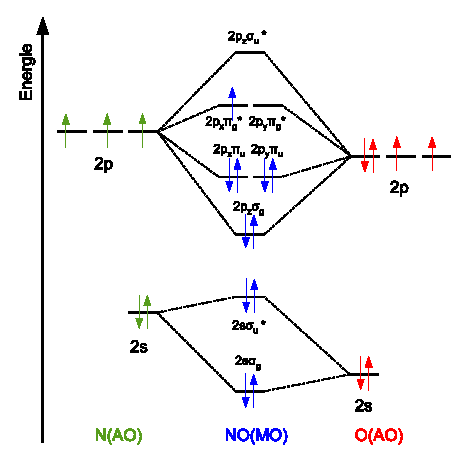
\includegraphics[scale=1]{NO-orbitaly.eps}
\caption[Orbitaly NO]{Orbitální diagram molekuly NO. Znázorněny jsou interakce pouze 2p a 2s orbitalů.}
\label{obr:NO-orbitaly}
\end{figure}

\noindent Jelikož je energie atomu dusíku nižší, budou MO vazebných orbitalů tvořeny z~větší míry právě orbitaly atomu N a na tom tak bude soustředěn větší záporný náboj. Všimněme si také, že molekula NO představuje dle tohoto schématu radikál.


Podívejme se ještě na jeden případ, na molekulu fluorovodíku. Elektron v~1s orbitalu atomu vodíku má energii -13,6 eV, elektron v~2p orbitalu atomu fluoru má hodnotu -17,4 eV. Orbitální diagram pak bude vypadat takto

\begin{figure} [htb]
\centering
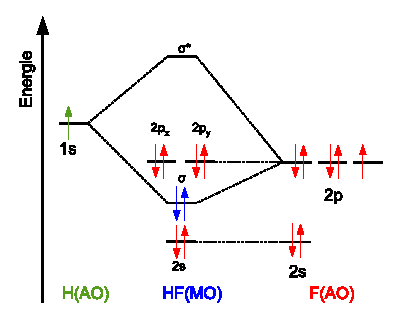
\includegraphics[scale=1]{HF-orbitaly.eps}
\caption[Orbitaly HF]{Orbitální diagram molekuly HF.}
\label{obr:HF-orbitaly}
\end{figure}

\noindent S~1s orbitalem atomu vodíku se ze symetrických důvodů může kombinovat pouze jediný z~2p orbitalů atomu fluoru. Zbylé dva orbitaly se vazby neúčastní, nejsou vazebné, ani antivazebné, nýbrž nevazebné. Opět vidíme, že vazebný orbital bude mít větší příspěvek  od atomu fluoru, konkrétně

\begin{equation}
\varphi_1 = 0{,}34 \cdot \orbital{1}{s}{\mathrm{H}} + 0{,}84 \cdot \orbital{2}{p_z}{\mathrm{F}},
\label{rov:ElStrukt-22}
\end{equation}


\noindent naopak antivazebný orbital bude mít větší příspěvek od atomu vodíku

\begin{equation}
\varphi_2 = 0{,}44 \cdot \orbital{1}{s}{\mathrm{H}} - 0{,}63 \cdot \orbital{2}{p_z}{\mathrm{F}},
\label{rov:ElStrukt-23}
\end{equation}


\noindent jelikož v~základním stavu elektrony nevazebný orbital nezaplňují, bude větší elektronová hustota lokalizovaná na atomu fluoru, a ten tak bude mít záporný parciální náboj. Tento typ úvah je základem tzv. Mullikenovy populační analýzy, o~které na přednášce bude řeč ještě později.
%% Tady by se asi dalo zmínit, že to souhlasí s elektronegativitou...


%DHnote: Následující odstavec mi přijde strašně matoucí, proč najednou hovoříme o řešení pro atomy?
Na závěr tohoto oddílu si ještě zopakujme, jakým způsobem přistupujeme k~řešení $N$-elektronové Schr\"odingerovy rovnice v~rámci přístupu MO-LCAO. Předpokládáme, že známe řešení pro orbitaly atomů vodíkového typu (tyto funkce přitom mohou obsahovat určité variační parametry). Jejich uspořádáním do Slaterova determinantu vytvoříme mnohaelektronovou vlnovou funkci a v~rámci metody Hartreeho-Focka tak vypočítáme elektronovou energii atomů. Jednoelektronové vlnové funkce atomů vodíkového typu můžeme v~rámci přístupu MO-LCAO zkombinovat do molekulových orbitalů, ze kterých pak vytvoříme opět mnohaelektronovou vlnovou funkci uspořádáním do Slaterova determinantu, viz. obrázek~\ref{obr:MOLCAO}.

\begin{figure} [htb]
\centering
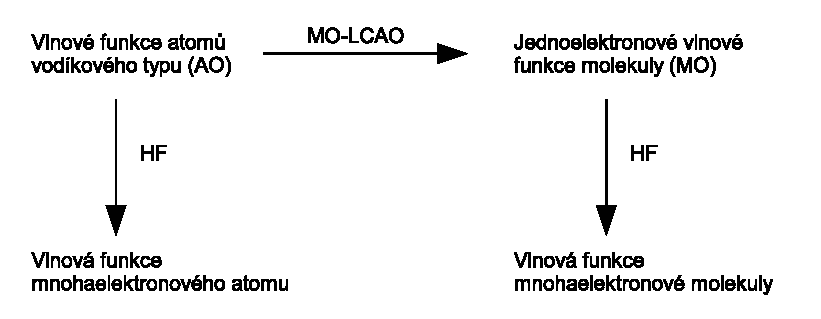
\includegraphics[scale=1]{Metoda-MO-LCAO.eps}
\caption{Metoda MO-LCAO}
\label{obr:MOLCAO}
\end{figure}


\subsection{Klasifikace molekulových orbitalů a elektronové termy dvouatomových molekul}
 
Jednoelektronové vlnové funkce molekul, tj. molekulové orbitaly, můžeme klasifikovat s~ohledem na chování vlnové funkce vůči prvkům symetrie molekul. Všechny diatomické molekuly mají nekonečně četnou osu symetrie $C_\infty$. Homonukleární diatomika mají navíc střed symetrie.

Z~hlediska chování vlnové funkce vůči ose symetrie $C_\infty$ mluvíme o 

\begin{itemize}

\item Orbitalu $\sigma$, jestliže rotace kolem osy $C_\infty$ ponechá orbital nezměněn.

\item Orbitalu $\pi$, jestliže je osa $C_\infty$ obsažena v~jedné uzlové rovině (tj. v~rovině, ve které je hodnota vlnové funkce nulová)

\item Orbitalu $\delta$, jestliže je osa $C_\infty$ obsažena ve dvou uzlových rovinách. 

\end{itemize}

\noindent A~takto bychom mohli pokračovat dále. Z~hlediska středu symetrie můžeme orbitaly klasifikovat jako 

\begin{itemize}

\item g (údajně z~něm. \textit{gerade}), kdy operace zrcadlení dle středu symetrie nemění znaménko vlnové funkce

\item u~(údajně z~něm. \textit{ungerade}), kdy operace zrcadlení dle středu symetrie mění znaménko vlnové funkce 

\end{itemize}

Na obrázku~\ref{obr:KlasifikaceMO} je klasifikace orbitalů znázorněna na několika příkladech.

\begin{figure} [htb]
\centering
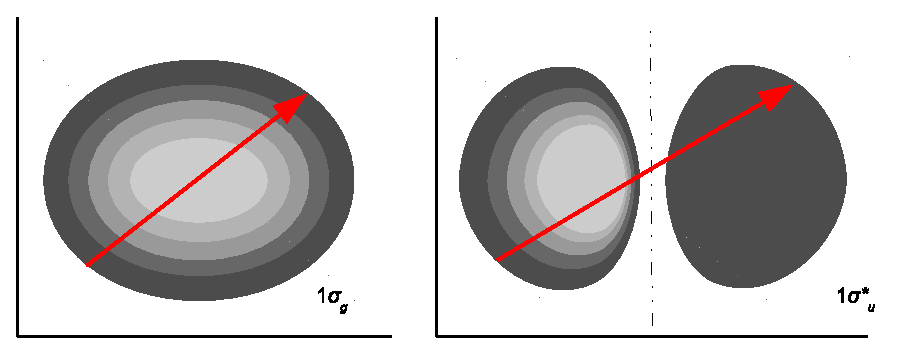
\includegraphics[scale=.8]{KlasOrbitaly.eps}
\caption[Klasifikace MO]{Příklad klasifikace molekulových orbitalů.}
\label{obr:KlasifikaceMO}
\end{figure}
 

Pojďme se ještě zamyslet nad otázkou, zda klasifikace orbitalů dle symetrie nemá ještě nějaký hlubší význam. Symetrie je obvykle znakem zachování určité fyzikální veličiny. U~molekul už nemůžeme předpokládat zachování momentu hybnosti jako u~atomů, neboť elektrony v~molekulách se nepohybují v~centrálním poli. Molekuly mají pořád ještě válcovou symetrii a~zachovává se tak průmět momentu hybnosti do osy $z$, $L_z$. Zavedeme-li si nyní kvantové číslo $\lambda= |m|$, kde $m=0,+-1,+-2$ atd., můžeme udělat následující přiřazení


\begin{table} [htb]
\centering
\begin{tabular}{c|c|c|c|c|c}
\toprule
$\lambda$ & 0 & 1 & 2 & 3 & 4\\
\midrule
označení & $\sigma$ & $\pi$ & $\delta$ & $\phi$ & $\gamma$\\
\bottomrule
\end{tabular}
\end{table}


Ve vícelektronových molekulách se moment hybnosti ve směru osy $z$ může sčítat. Celkové magnetické kvantové číslo $M_L$ vícelektronové molekuly je pak dáno prostým součtem magnetických kvantových čísel $m$ jednotlivých elektronů. Zavádíme pak kvantové číslo 

\begin{equation}
\Lambda = \vert M_L \vert
\label{rov:ElStrukt-24}
\end{equation}   
      
\noindent a opět zavádíme značení


\begin{table} [H]
\centering
\begin{tabular}{c|c|c|c|c|c}
\toprule
$\Lambda$ & 0 & 1 & 2 & 3 & 4\\
\midrule
označení & $\Sigma$ & $\Pi$ & $\Delta$ & $\Phi$ & $\Gamma$\\
\bottomrule
\end{tabular}
\end{table}

\begin{priklad}
\textbf{Zadání A:} Mějme konfiguraci $\sigma\sigma$. Určete možné stavy této molekuly.\\[0.1cm]
\textbf{Řešení A:} 
\begin{displaymath}
^{1}\Sigma, \, ^{3}\Sigma.
\end{displaymath}

\textbf{Zadání B:} Mějme konfiguraci $\pi\pi$. Určete možné stavy této molekuly.\\[0.1cm]
\textbf{Řešení B:}
\begin{displaymath}
^{1}\Sigma, \, ^{3}\Sigma, \, ^{1}\Delta, \, ^{3}\Delta.
\end{displaymath} \vspace{-0.7cm}
\end{priklad}

Můžeme pak ještě uvažovat celkový moment hybnosti $\vec{\Omega}$ daný součtem orbitálního a spinového momentu molekuly. Odpovídající kvantové číslo nabývá hodnot

\begin{equation}
\Lambda + S, \, \Lambda + S - 1, \dots, \Lambda - S. 
\label{rov:ElStrukt-25}
\end{equation}

\begin{priklad}
\textbf{Zadání:} V~jakých stavech se může nacházet molekula ve stavu $^4\Pi$?\\[0.1cm]
\textbf{Řešení:}
\begin{displaymath}
^4\Pi_{5/2}, \, ^4\Pi_{3/2}, \, ^4\Pi_{1/2}, \, ^4\Pi_{-1/2}.
\end{displaymath} \vspace{-0.7cm}
\end{priklad}

Energetické rozštěpení těchto stavů je pro prvky o~malém protonovém čísle velmi malé, je dáno pouze spin-orbitální interakcí, o~které již byla řeč dříve. 


\subsection{Molekulové orbitaly víceatomových molekul}
Doposud jsme diskutovali pouze diatomické molekuly. Elektronovou energii můžeme ale prostřednictvím Hartreeho-Fockovy metody stejně dobře hledat i pro molekuly víceatomové. Opět budeme hledat molekulové orbitaly jako lineární kombinaci atomových orbitalů. Tyto molekulové orbitaly nemůžeme již klasifikovat s~ohledem na chování vůči ose symetrie $C_\infty$, neboť obecně molekuly takovouto symetrii nevykazují. I~nižší symetrie ale mohou sloužit k~označování molekulových orbitalů. Příklad molekulových orbitalů víceatomové molekuly lze najít na obrázku~\ref{obr:Voda_Orbitaly}.

\begin{figure} [htb]
\centering
\includegraphics[scale=.8]{Voda_Orbitaly.eps}
\caption{Molekulové orbitaly molekuly vody.}
\label{obr:Voda_Orbitaly}
\end{figure}

 
Všimněme si, že v~případě molekuly vody není tak úplně snadné říci, zda jde o~orbital vazebný či antivazebný. Příslušné molekulové orbitaly jsou totiž delokalizovány přes celou molekulu. Rozhodně se nedá říci, že určitý molekulový orbital náležel určité vazbě. Pro chemika to není úplně komfortní situace. Od dob Lewisových je zvyklý si chemickou vazbu představovat jako sdílený elektronový pár. Tento pár by se pak dle chemického pohledu měl nacházet někde mezi dvěma atomy, jako je to v~případě diatomických molekul. 

Tomuto pohledu v~principu není obtížné vyjít vstříc. Orbitaly jsou totiž pouze pomocnými veličinami, fyzikálně pozorovatelné veličiny závisí toliko na celkové vlnové funkci. Každá transformace orbitalu taková, že zanechá vlnovou funkci až na znaménko netknutou, je proto možná. Jak taková povolená transformace má vypadat? Zaveďme si tzv. unitární matici vztahem

\begin{equation}
\mathbf{U}^{\ast} \mathbf{U} = \mathbf{1}.
\label{rov:ElStrukt-26}
\end{equation}

\noindent Potom bude nutně platit

\begin{equation}
\mbox{det} \vert \mathbf{U}^{\ast} \vert \cdot \mbox{det} \vert \mathbf{U} \vert = \mathbf{1}.
\label{rov:ElStrukt-27}
\end{equation}

\noindent Z~čehož ale vyplývá, že 
%%tomuhle nerozumim. Z čeho to vyplývá, že tvar determinantu bude komplexni exponenciela??

\begin{eqnarray}
\mbox{det} \vert \mathbf{U} \vert &=& e^{i\lambda}, \nonumber \\
\mbox{det} \vert \mathbf{U}^{\ast} \vert &=& e^{-i\lambda},
\label{rov:ElStrukt-28}
\end{eqnarray}


\noindent kde $\lambda$ je libovolné číslo. Nyní si definujme matici 


\begin{equation}
\mathbf{A}=
\begin{pmatrix}
\phi_1(1) & \phi_1(2) & \ldots & \phi_1(N) \\
\vdots & \vdots & & \vdots \\
\phi_N(1) & \phi_N (2) & \ldots & \phi_N(N)
\end{pmatrix}.
\label{rov:ElStrukt-29}
\end{equation}


\noindent Hartreeho-Fockova vlnová funkce je pak dána jako


\begin{equation}
\psi(1,2, \dots, N) = \mbox{det} \mathbf{A}.
\label{rov:ElStrukt-30}
\end{equation}


\noindent Mějme nyní transformovanou sadu orbitalů


\begin{equation}
\begin{pmatrix}
\phi_1^{\prime} \\
\vdots \\
\phi_N^{\prime}
\end{pmatrix}
= \mathbf{U} 
\begin{pmatrix}
\phi_1 \\
\vdots \\
\phi_N
\end{pmatrix}.
\label{rov:ElStrukt-31}
\end{equation}


\noindent A~v~této sadě napišme Slaterův determinant

\begin{equation}
\psi^{\prime}(1,2, \dots, N) = \mbox{det} ( \mathbf{U} \cdot \mathbf{A}).
\label{rov:ElStrukt-32}
\end{equation}

\noindent Z~čehož 

\begin{equation}
\psi^{\prime}(1,2, \dots, N) = e^{i \lambda} \psi(1,2, \dots, N).
\label{rov:ElStrukt-33}
\end{equation}

\noindent Pro reálné vlnové funkce faktor $e^{i\lambda}$  neznamená než změnu znaménka.
%DHnote opravdu? Pokud je lambda jakakoli cislo, tak se jedna spise o zmenu faze, ne? 
Vidíme tedy, že jakákoliv unitární transformace orbitalů nevede k~závažné změně vlnové funkce. Transformovaná sada orbitalů je stejně dobrou sadou jako ta původní. Nikdo nám proto nemůže zabránit ve vytvoření sady atomových orbitalů, která v~případě tetraedrického uspořádání vazeb, jako v~případě molekuly vody, povede ke čtyřem orbitalům mířícím do vrcholu tetraedru


\begin{eqnarray}
\phi^{\prime}_1 &=& \frac{1}{2} ( 2 \mathrm{s} + 2 \mathrm{p_x} + 2 \mathrm{p_y} + 2 \mathrm{p_z}) \quad \phi^{\prime}_3 = \frac{1}{2} ( 2 \mathrm{s} + 2 \mathrm{p_x} - 2 \mathrm{p_y} - 2 \mathrm{p_z}), \nonumber \\
\phi^{\prime}_2 &=& \frac{1}{2} ( 2 \mathrm{s} - 2 \mathrm{p_x} - 2 \mathrm{p_y} + 2 \mathrm{p_z}) \quad \phi^{\prime}_4 = \frac{1}{2} ( 2 \mathrm{s} - 2 \mathrm{p_x} + 2 \mathrm{p_y} - 2 \mathrm{p_z}).
\label{rov:ElStrukt-34}
\end{eqnarray}


Tyto tzv. \textbf{hybridní orbitaly} je možné využít ke konstrukci molekulových orbitalů molekuly vody (či kupříkladu molekuly methanu). Získané orbitaly se budou nacházet v~oblasti vazeb. Jde ale o~změnu víceméně kosmetickou a není žádoucí pojem hybridizace přeceňovat. Poznamenejme, že původní, tzv. kanonické, orbitaly jsou v~jistém smyslu \uv{fyzikálnější}, neboť pouze pro ně (a nikoliv pro hybridní orbitaly) platí Koopmansův teorém.
\footnote{K diskuzi o~hybridních orbitalech odkazujeme na starší článek A. Sadleje a R. Zahradníka \textit{Jsou chemické jevy podmíněné hybridizací?} Chem. Listy \textbf{1981}, 75, 561-562, stejně jako na nedávnou zajímavou výměnu názorů iniciovanou textem A. Grushowa \textit{\uv{Is It Time To Retire the Hybrid Atomic Orbital?}} J. Chem. Educ. \textbf{2011}, 88, 860-862.}
Pro případ orbitalů \eqref{rov:ElStrukt-34} má matice $\mathbf{U}$ tvar

\begin{equation}
\mathbf{U} = 
\begin{pmatrix}
1 & 1 & 1 & 1 \\
1 & -1 & -1 & 1 \\
1 & 1 & -1 & -1\\
1 & -1 & 1 & -1
\end{pmatrix}.
\end{equation}

\noindent Snadno se přesvědčíme, že matice je skutečně unitární.



\clearpage
\section{Ab initio metody}
\label{kap:abinitio}
V~této kapitole se vrátíme k~základní úloze kvantové chemie, tj. k~řešení elektronové Schr\"{o}dingerovy rovnice pro danou molekulu. Ukážeme si, jak tuto rovnici můžeme v~principu obecně řešit pro atomy a~molekuly.  Existují v~zásadě tři přístupy k~tomuto problému:

\begin{itemize}

\item \textit{Ab initio} metody.  Schr\"{o}dingerovu  rovnici řešíme pomocí hierarchie různě chytrých aproximací (obvykle přitom začínáme Hartreeho-Fockovou metodou) bez dodatečných parametrů. Tyto metody se nazývají \textit{ab initio} (z~lat. \uv{\it{od počátku}}), jelikož k~výpočtům potřebujeme dopředu znát pouze základní fyzikální konstanty jako je hmotnost a náboj elektronu nebo Planckova konstanta. 

\item Semiempirické metody. Tyto metody jsou založeny na principech kvantové mechaniky, některé parametry (typu coulombický či rezonanční integrál) se ale přímo nepočítají, ale nastavují se buď z~experimentálních dat nebo z~přesnějších \textit{ab initio} výpočtů.

\item Metody založené na teorii funkcionálu hustoty.  Teorie funkcionálu hustoty (DFT, z~angl. \textit{Density Functional Theory}) představuje fundamentálně odlišný přístup od předchozích dvou. Není založen na hledání vlnové funkce, ale soustředí se na mnohem jednodušší veličinu -- elektronovou hustotu. DFT metoda je často řazena mezi \textit{ab initio} metody, jelikož v~principu vede k~přesnému řešení a praktická přesnost je taktéž na úrovni \textit{ab initio} metod. Na druhou stranu ale většina DFT metod obsahuje několik empirických parametrů (mnohem méně než semiempirické metody), které se často fitují na experimentální data.

\end{itemize}

V~této kapitole se zaměříme na \textit{ab initio} metody, metody založené na funkcionálu hustoty a~semiempirické metody probereme v~následujících kapitolách. Nejjednodušší \textit{ab initio} metodou je metoda Hartreeho--Fockova, která již byla stručně představena v~kapitolách \ref{kap:viceelektron} a \ref{kap:elstruktmol}.
V~praxi se dnes používá spíše méně, ale stále slouží jako odrazový můstek pro většinu ostatních přesnějších \textit{ab initio} metod, tudíž si ji zde zopakujeme a probereme hlouběji.

Bude užitečné ujasnit si na začátku notaci užitou v~této kapitole, abychom se ve všech těch řeckých písmenech neztratili. Celkovou vlnovou funkci budeme značit symbolem $\psi$,  zatímco molekulové \textbf{spinorbitaly} (MO) budeme značit $\varphi$. Každý MO je součinem \textbf{prostorové části} $\phi$ a \textbf{spinové části} $\alpha$ nebo $\beta$. V~rámci aproximace MO-LCAO poté každou prostorovou část MO rozvíjíme do báze \textbf{atomových orbitalů} $\chi_i$. Abychom si ušetřili práci s~psaním rovnic, budeme v~této kapitole důsledně využívat atomové jednotky. Počet elektronů značíme $N$ a~počet jader~$K$.

\begin{table}[ht]
\centering
\caption{Základní symboly použité v~následujících kapitolách.}
\begin{tabular}{|c|l|c|}
\hline 
\rule[-1ex]{0pt}{2.5ex} Symbol & 	Význam	& Vlastnosti \\ 
\hline 
\rule[-1ex]{0pt}{2.5ex} $\psi$ & Celková el. vln. funkce  & $\psi$ = $det|\phi_1 \phi_2 \cdots \phi_N |$ \\ 
\hline 
\rule[-1ex]{0pt}{2.5ex} $\varphi$ & Molekulový orbital & $\varphi_i=\phi_i \alpha $\\ 
\hline 
\rule[-1ex]{0pt}{2.5ex} $\phi$ & Prostorová část MO & $\phi_i=\sum_{j=1}^N \chi_j $ \\ 
\hline 
\rule[-1ex]{0pt}{2.5ex} $\alpha$, $\beta$  & Spin--orbitaly & \\ 
\hline 
\rule[-0ex]{0pt}{2.5ex} $\chi$ & atomové orbitaly & $\int |\chi|^2 \mathrm{d}\textbf{r} = 1 $ \\
\hline
\end{tabular} 
\label{tab:vlnfunkce}
\end{table}

\subsection{Hartreeho-Fockova metoda}

Zopakujme si nejprve základní teze Hartreeho-Fockovy teorie. Začneme tím, že celkovou vlnovou funkci předpokládáme ve formě Slaterova determinantu (SD)
\begin{equation}
\psi^{HF}=\frac{1}{\sqrt{N!}}\begin{vmatrix}
\varphi_1(1) & \varphi_1(2) & \cdots & \varphi_1(N) \\
\varphi_2(1) & \varphi_2(2) & \cdots & \varphi_2(N) \\
\vdots & \vdots & \vdots & \vdots \\
\varphi_N(1) & \varphi_N (2) & \cdots & \varphi_N(N)
\end{vmatrix}.
\end{equation}
Jelikož SD má $N!$ členů, kde $N$ je počet elektronů, je třeba použít normalizační faktor $\frac{1}{\sqrt{N!}}$. Vlnová funkce ve tvaru součinu nám říká, že předpokládáme nezávislý pohyb elektronů (v~poli jader a ve zprůměrovaném poli ostatních elektronů).

Optimální jednoelektronové vlnové funkce, tj. molekulové orbitaly, získáme pomocí variačního principu. Funkcionál energie v~rámci metody HF má tvar 
\begin{equation}
E^{HF}= \sum_{i=1}^N H_{ii}+ \frac{1}{2}\sum_{i\neq j} \left( J_{ij}-\delta(s_{i},s_{j})K_{ij} \right),
\label{rov:abinitio:ehf}
\end{equation}
kde $H_{ii}$ je maticový člen popisující jednoelektronové příspěvky k~energii (tj. kinetickou energii elektronů a interakci elektronů s~jádry), $J_{ii}$ je coulombovský integrál a $K_{ij}$ je výměnný integrál.
Jako argument u~Kroneckerovy delty $\delta(s_{i},s_{j})$ jsou uvedeny spinová čísla elektronů. Z~toho vyplývá, že výměnná interakce se uplatňuje pouze mezi elektrony se stejným spinem.
Tento vztah byl odvozen za předpokladu, že jsou molekulové orbitaly ortogonální. Tento požadavek je ryze praktického rázu, ke stejnému výsledku bychom došli i bez něj, ale mnohem obtížněji. Také si můžeme všimnout, že jsme se již integrací zbavili spinové části spinorbitalu a dále pracujeme jen s~prostorovou částí MO.

Aplikací variačního počtu na předchozí rovnici (více o~funkcionálech a variacích si povíme v~kapitole o~DFT) dostaneme Fockovy rovnice\footnote{Ve skutečnosti hledáme vázaný extrém, jelikož musíme zachovat podmínku ortonormality MO, z~níž byl odvozen vztah \ref{rov:abinitio:ehf}.} 
\begin{equation}
\hat{F}\phi_i(1) = \epsilon_i \phi_i ,
\label{rov:abinitio:fockrov}  
\end{equation}
kde Fockův operátor $\hat{F}$ má tvar
\begin{equation}
\hat{F}_i = \hat{h}_i+\sum^N_{j(\neq i)} \left(\hat{J}_j - \delta(s_i,s_j) \hat{K}_j \right) .
\label{rov:abinitio:fockoper}
\end{equation}
%je treba zduraznit, ze ta suma neni dvojna, narozdil od vztahu pro energii
První člen zahrnuje  kinetickou energii $i$-tého elektronu a jeho přitažlivou interakci s atomovými jádry dle vztahu
\begin{equation}
\hat{h}_i = -\frac{1}{2}\Delta_i - \sum_{A}\frac{Z_A}{r_{iA}} .
\end{equation}
Zbylé dva členy popisuji coulombickou a výměnnou interakci $i$-tého elektronu se zprůměrovaným polem ostatních elektronů:
\begin{eqnarray}
\hat{J}_j=\int \frac{|\phi_j |^2}{|\textbf{r}_{i}-\textbf{r}_{j}|}\mathrm{d}\textbf{r}_j \\
\hat{K}_{ij} = \int \frac{\phi_j^*(\mathbf{r}_j)\phi_i(\mathbf{r}_i)}{|\textbf{r}_{i}-\textbf{r}_{j}|}\mathrm{d}\textbf{r}_j .
\end{eqnarray}

Fockovy rovnice jsou složité integro-diferenciální rovnice pro neznámé funkce $\phi_i$,
což jsou naše hledané molekulové orbitaly.
Tyto rovnice typicky řešíme rozvojem molekulových orbitalů do báze orbitalů atomových
\begin{equation}
\phi_i=\sum_{j=1}^K c_{ij} \chi_j ,
\end{equation}
kde $K$ je počet AO v~naší bázi. Tím se problém rapidně zjednoduší, jelikož nyní nehledáme funkce, ale jen číselné koeficienty $c_{ij}$, které vyjadřují příspěvek $j$-tého atomového orbitalu k~$i$-tému molekulovému orbitalu.
Výsledné rovnice se nazývají Roothanovy, což jsou následující algebraické rovnice
\begin{equation}
\mathbf{F} \mathbf{c} = \varepsilon \mathbf{S} \mathbf{c} .
\end{equation}

Jelikož molekuly jsou složeny z~atomů, vhodnou bází jsou atomové orbitaly.
Dnes se již téměř výhradně používají Gaussovy funkce, o~kterých již byla řeč v~kapitole \ref{sec:AObasis}.
Pokud bychom použili nekonečně velkou bázi, získali bychom tzv. \textbf{Hartreeho--Fockovu limitu} a naše MO by měli nejlepší možný tvar. Tato limita ale \textbf{není} přesné řešení elektronové Schr\"{o}dingerovy rovnice!
Předpokládali jsme totiž vlnovou funkci ve tvaru Slaterova determinantu. Tato vlnová funkce ale trpí principiálními defekty. V~přesné vlnové funkci by se nám třeba nikdy nemohlo stát, že bychom nalezli dva elektrony na jednom místě, takovéto uspořádání by totiž dle Coulombova zákona mělo nekonečnou energii.
Na tomto místě je dobré si uvědomit, že celý koncept molekulových orbitalů, na které jsou chemici již tak zvyklí, je založen na HF teorii, a je tudíž pouze aproximací. Jakmile se budeme snažit dosáhnout přesnějších výsledků, začne se nám úhledný obrázek elektronů sedících v~molekulových orbitalech rozpadat.

Jelikož je HF metoda metodou variační, je energie HF limity vyšší než skutečná energie získaná přesným řešení nerelativistické Schr\"{o}dingerovy rovnice.
Rozdíl mezi těmito dvěma metodami se nazývá korelační energie
\begin{equation}
E_{kor}=E_{el} - E^{HF}
\end{equation}
a je důsledkem toho, že jsme zanedbali okamžitou mezi-elektronovou repulzi.

%OBRAZEK, znazorneni HF limity, kor. energie, presneho reseni a relativistickeho reseni

%TODO: zminit resitricted a unrestricted pripady

Pro výpočet korelační energie je třeba použít pokročilejších metod, které popíšeme v~následujících kapitolách.

\subsection{Poruchový přístup: M\o llerova-Plessetova metoda}
HF metoda popisuje nezávisle se pohybující elektrony. Skutečné elektrony se úplně nezávisle nepohybují, jejich pohyb je korelován. Rozdíl mezi HF elektrony a skutečnými elektrony ale obvykle není příliš velký, takže bychom mohli použít poruchovou teorii.  Existují různé cesty k~poruchovému řešení elektronové Schr\"{o}dingerovy rovnice, nejčastěji se setkáváme s~metodou, kterou zavedli dánští badatelé M\o ller a Plesset.

V~poruchové metodě je třeba nejprve najít problém, který jsme schopni řešit a který je dostatečně blízko přesnému řešení. K~tomuto zde využijeme HF teorie. Nyní je třeba vymyslet, jaký je vlastně hamiltonián HF metody, abychom poté podle rovnice \eqref{rov:approx:ham} mohli skutečný hamiltonián rozdělit na poruchu a HF hamiltonián
\begin{equation}
\hat{H}^{\prime}_{MP}=\hat{H}_{el} - \hat{H}^{(0)}_{HF} .
\end{equation}

Jelikož Fockovy rovnice \ref{rov:abinitio:fockrov} jsou rovnicemi jednoelektronovými, bude se celkový hamiltonián skládat ze součtu jednoelektronových Fockových operátorů \ref{rov:abinitio:fockoper}
\begin{equation}
\hat{H}^{(0)}_{HF}= \sum_{i=1}^N \hat{F}_i.
\label{rov:abinitio:hfham}
\end{equation}
Energie tohoto hamiltoniánu je potom rovna součtu orbitálních energií
\begin{equation}
E^{(0)}_{HF}=\sum_{i=1}^N \epsilon_i .
\end{equation}
Pozor, toto není HF energie! V~součtu orbitálních energií jsou mezielektronové interakce započteny dvakrát. Nyní můžeme přejít k~definici naší poruchy odečtením rovnice \eqref{rov:abinitio:hfham} od elektronového hamiltoniánu. Jednoelektronové členy se vyruší a vyjde nám
\begin{equation}
\hat{H}^{\prime}_{MP}=\hat{H}_{el}-\hat{H}^{(0)}_{HF}= \sum_{j\neq i}^{N} \frac{1}{\textbf{r}_{ij}} - \left(\sum_{j\neq i} \left( \hat{J}_j - \delta(s_i,s_j) \hat{K}_j \right) \right) .
\end{equation}
Vidíme, že porucha je dána rozdílem mezi coulombickým členem a efektivním polem elektronů v~HF teorii.

Zkusme si nyní podle vzorce \eqref{rov:PorusenaEnergie} vypočítat energii do prvního řádu. Platí, že
\begin{equation}
E_1=E^{(0)}_{HF} + E^{(1)}= \sum_{i=1}^N \epsilon_i - \left(\sum_{j\neq i}^{N} \left( J_{ij} - \delta(s_i,s_j) {K}_{ij} \right) \right).
\end{equation}
%TODO: podobny vzorec bychom meli ukazat uz v predchozi kapitole
To jsme se daleko nedostali! Porucha v~prvním řádu nám ve výsledku dá původní HF energii.
Užitečná je tedy až porucha druhého řádu, pro kterou ze vzorce \eqref{rov:aprox:energiePT2} platí:
\begin{equation}
E^{MP2} = E^{HF} + \sum_m \frac{\left < \psi^{(0)}_{HF}|\hat{H}^{\prime}_{MP}|\psi_n^{(0)} \right >}{E_{HF}^{(0)}-E_m^{(0)}}.
\end{equation}

Vypadá to, že budeme muset počítat spoustu maticových elementů mezi základním stavem a všemi excitovanými Slaterovými determinanty (o~těch si více povíme v~další podkapitole). Naštěstí se dá ukázat (díky tzv. Brillouinovu\footnote{Toto jméno vysloví opravdu jen zkušení frankofilové.} teorému a Slaterovým-Condonovým pravidlům), že většina z~nich bude nulová a přispívat budou jen dvojitě-excitované determinanty, které zde zjednodušeně značíme $\psi_{ij}^{rs}$ (excitujeme dva elektrony z~orbitalů $i$ a $j$ do orbitalů $r$ a $s$). Výsledný vzorec tudíž bude
\begin{equation}
E^{MP2}= E^{HF} + \sum_{ij} \sum_{rs} \frac{\left < \psi_0 | \hat{H}^{\prime}_{MP} | \psi_{ij}^{rs} \right > }{\epsilon_r+\epsilon_s-\epsilon_i-\epsilon_j} .
\end{equation}
Metoda zahrnující příspěvky do druhého řádu teorie poruch má zkratku MP2 a je jednou z~nejvíce užívaných metod na výpočet korelační energie. Mohli bychom pokračovat a odvodit vzorce pro vyšší řády a dostali bychom pak metody MP3, MP4 atd. 
Metoda MP3 nepřináší výrazné zlepšení oproti MP2 a tudíž není využívána. Metoda MP4 je velmi přesná, ale také velmi výpočetně náročná. Ani ona se v~dnešní době příliš nevyužívá, pro velkou přesnost je totiž výhodnější použít metody spřažených klastrů, o~kterých bude řeč za chvíli.


\subsection{Metoda konfigurační interakce}

Alternativní cestu ke korelační energii nabízí variační princip. Dá se ukázat, že množina všech Slaterových determinantů, které můžeme vytvořit z~HF molekulových orbitalů, vytváří úplný soubor funkcí. Můžeme tak do něj rozvinout přesnou vlnovou funkci 
\begin{equation}
\psi^{CI}=C_0\psi_0+\sum_a\sum_m C_a^m\psi_a^m+\sum_m \sum_n \sum_a \sum_b C_{ab}^{mn}\psi_{ab}^{mn}+\dots \quad ,
\label{rov:CIrozvoj}
\end{equation}
kde první člen je Slaterův determinant základního stavu a další členy odpovídající determinantům, kde jsme excitovali jeden nebo více elektronů z~obsazeného do neobsazeného orbitalu (viz obrázek \ref{obr:abinitio:ci}). Druhý člen odpovídá jednonásobným excitacím (monoexcitacím, viz obr. \ref{obr:abinitio:ci}A), třetí člen odpovídá dvojnásobným excitacím (biexcitacím,
viz obr.\,\ref{obr:abinitio:ci}B) atp. Jednotlivým Slaterovým determinantům můžeme také říkat konfigurace, odtud název metody konfigurační interakce (CI, z~angl. \textbf{Configuration Interaction}).

\begin{figure} [htb]
\centering
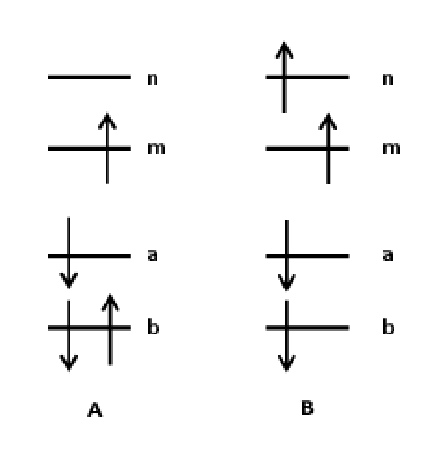
\includegraphics[scale=1]{CIkonfigurace.eps}
\caption[Excitované elektronové konfigurace]{Ukázka monoexcitovaných (\textbf{A}) a biexcitovaných (\textbf{B}) konfigurací.}
\label{obr:abinitio:ci}
\end{figure}

Jak nyní určíme koeficienty $C_i$ (pozor, neplést s~koeficienty u atomových orbitalů $c_ij$ v~HF metodě)? Opět pomocí variačního principu. Jelikož vlnová funkce na těchto koeficientech závisí lineárně, aplikací variačního principu dostaneme již mnohokrát zmíněné sekulární rovnice
\begin{equation}
\mathbb{H}\mathbf{C}=E\mathbb{S}\mathbf{C} \nonumber ,\\
\end{equation}
%\sum_j (H_ij-E_i\delta_{ij})C_i=0 \quad \forall i
kde maticové elementy $H_{ij}$ představují integrály mezi Slaterovými determinanty

\begin{equation}
H_{ij}= \left\langle \psi_i | \hat{H}_{el} | \psi_j \right\rangle.
\end{equation}

Výsledné matice $\mathbb{H}$ mohou být často obrovské (rozměr milion x milion není vůbec šokující), ale existují efektivní metody výpočetní lineární algebry, které si s~nimi dokáží poradit. Hlavní trik je v tom, že většina elementů v této matici je nulových, mluvíme o tzv. řídké matici. 

Pokud bychom použili nekonečnou bázi AO a zahrnuli všechny možné Slaterovy determinanty (kterých by bylo taktéž nekonečně mnoho), dostali bychom přesné řešení Schr\"{o}dingerovy rovnice. V~praxi ale musíme použít bázi konečnou, máme tedy i konečný počet molekulových orbitalů. Pokud v~rámci této báze budeme uvažovat všechny možné Slaterovy determinanty, mluvíme o~metodě úplné konfigurační interakce (FCI, z~angl. \textit{Full Configuration Interaction}). Zvětšováním báze se metoda FCI může libovolně přiblížit přesnému řešení. Metoda FCI je ale extrémně výpočetně náročná (náročnost roste exponenciálně s~počtem orbitalů) a lze ji tedy použít pouze pro malé molekuly s~malou bází.

Pro praktické výpočty tedy musíme počet excitací omezit. Pokud se omezíme pouze na jednonásobné a dvojnásobné excitace, získáme metodu CISD (z~angl. \textit{Configuration Interaction Singles Doubles}), která byla v~minulosti hojně využívána.

Dnes se metody konfigurační interakce užívají méně, jelikož mají některé nevýhody oproti jiným metodám. 
\begin{itemize}
\item Metoda FCI je sice přesná, ale v~praxi díky exponenciálnímu škálování nepoužitelná.
\item Rozvoj \ref{rov:CIrozvoj} konverguje velmi pomalu. Pro dobrou přesnost bychom chtěli minimálně čtyřnásobné excitace.
\item Pokud použijeme konečný rozvoj \ref{rov:CIrozvoj}, tak výsledná metoda nemá správnou závislost na velikosti systému (v~žargonu kvantových chemiků, metoda není \uv{size konsistentní}). Co tento pojem znamená? Zjednodušeně řečeno, pokud metoda není \uv{size konsistentní}, tak její přesnost bude záviset na velikosti systému. Pro malou molekulu můžeme například metodou CISD zachytit přes 90 \% korelační energie, ale pro větší molekulu mnohem méně. Pro \uv{size konsistentní} metodu by mělo platit, že energie dvou nekonečně vzdálených molekul by měla být přesně rovna dvojnásobku energie jedné molekuly. Na příkladu dvou atomů helia lze ale snadno ukázat, že toto pro metodu CISD není splněno. Pro jeden atom He totiž metoda CISD odpovídá metodě FCI, jelikož máme pouze dva elektrony, které můžeme excitovat. Pro dva nekonečně vzdálené atomy helia již ale toto neplatí, jelikož máme už čtyři elektrony a některé Slaterovy determinanty tudíž nebudou v~CISD metodě zahrnuty. 
%(\textbf{obrázek? PSnote: Ano})
Metoda MP2 či metoda spřažených klastrů \uv{size konsistentní} jsou, metoda CI naopak nikoliv. 
\end{itemize}


\subsection{Metody spřažených klastrů}
Metody spřažených klastrů (CC, z~angl.\textit{Coupled Cluster}) nesou od svého počátku českou stopu. Tyto metody totiž použil v~kontextu kvantové chemie poprvé Jiří Čížek a později také Josef Paldus. Metoda spřažených klastrů je založena na mazaném přeskládání rozvoje typu CI. Klíčovým pojmem v~této metodě jsou takzvané excitační operátory. Například operátor $\hat{T}_1$ působí na vlnovou funkci základního stavu jako
\begin{eqnarray}
\hat{T}_1\psi_0=\sum^N_{a=1}\sum_{m=n+1}^\infty t_a^m\psi_a^m , 
\end{eqnarray}
tj. generuje lineární kombinaci mono-excitovaných konfigurací.  Tento operátor obsahuje neurčené koeficienty $t_a^m$ (tzv. \textbf{amplitudy}) popisujících zapojení jednotlivých excitovaných konfigurací do celkové vlnové funkce. Obdobně operátor $\hat{T}_2$ 
\begin{eqnarray}
\hat{T}_2\psi_0=\sum_{a=1}^N \sum_{b\neq a}^N\sum_{m=N+1}^\infty \sum_{n=N+1}^\infty t_{ab}^{mn}\psi_{ab}^{mn}
\end{eqnarray}
generuje lineární kombinaci  bi-excitovaných konfigurací atp. Celkový excitační (klastrový) operátor píšeme jako
\begin{eqnarray}
\hat{T}=\hat{T}_1+\hat{T}_2+\cdots \hat{T}_N.
\end{eqnarray}

Vlnovou funkci v~rámci metody spřažených klastrů zapisujeme v~poněkud neobvyklém tvaru
\begin{eqnarray}
\psi^{CC} = e^{\hat{T}} \psi_0 ,  \\
\end{eqnarray}
kde $\psi_0$ je referenční funkce, většinou z~metody HF. Zde se poprvé setkáváme s~pojmem exponenciály operátoru. Není třeba se jej leknout, jen si musíme uvědomit, jak je vlastně definována normální exponenciální funkce $e^x$. Exponenciální funkci čísla můžeme definovat pomocí Taylorova rozvoje
\begin{equation}
e^x=\sum_{i=1}^\infty \frac{x^n}{n!} .
\end{equation}
Tu samou definici nyní můžeme snadno aplikovat i na operátory, musíme jen vědět, jak operátory umocňovat.
To jsme si ale řekli již v~kapitole \ref{kap:OperaceSOperatory}. Operátor umocněný na $n$-tou prostě znamená, že jej aplikujeme $n$-krát za sebou na tu samou funkci. Exponenciála excitačního operátoru tedy vyjde jako 
\begin{equation}
e^{\hat{T}} = 1+\hat{T}+\frac{\hat{T}^2}{2}+\cdots.
\end{equation}
Díky vlastnostem excitačního operátoru je tato řada konečná, neboť molekula má pouze konečný počet elektronů, které lze excitovat.

Jaká je vlastně výhoda takto složitého zápisu?
Pokud použijeme úplný excitační operátor, tak dojdeme k~exaktnímu řešení stejně jako metodou FCI. Budeme ale potřebovat stejné množství parametrů, ať už je nazýváme rozvojovými koeficienty (v~metodě CI) nebo amplitudami (v~metodě CC).
Výhody se ale objeví, když excitační operátor začneme ořezávat. Když například vezmeme v~potaz pouze mono- a bi-excitace, dostaneme metodu CCSD  (z~angl. \textit{Coupled Cluster Singles Doubles}).
Na rozdíl od metody CISD je ovšem CCSD \uv{size-konzistentní} a navíc dostaneme větší podíl korelační energie.
To je dáno právě speciálním tvarem CC vlnové funkce, díky kterému i na úrovni CCSD dostaneme například i přibližný příspěvek čtyřnásobných excitací, jelikož v~exponenciální řadě je přítomen operátor $\hat{T}_2^2$. Stačí nám přitom stejný počet parametrů jako v~metodě CISD.

Vzorec pro energii v~rámci metod typu CC je složitější, poněkud náročnější jsou také pracovní rovnice této metody určující amplitudy $t$ klastrového operátoru. Metody spřažených klastrů jsou stejně jako poruchové metody size-konzistentní a obdobně nejsou variační. Ukazuje se ale, že v~praxi je právě správná závislost na velikosti systému důležitější, a proto se metody konfigurační interakce dnes používají méně často než poruchové metody a metody spřažených klastrů.

Jak jsme si již řekli v~předchozí podkapitole, metody konfigurační interakce konvergují dosti pomalu k~přesnému řešení. Tvar vlnové funkce v~metodě spřažených klastrů tuto konvergenci značně urychluje. Už se zahrnutím trojitých excitací dostáváme výsledky s~chemickou přesností (tzn. relativní energie s~přesností 1\,kcal/mol, což je zhruba 4\,kJ/mol).
Metoda CCSD(T) je v~současné době považována za \uv{zlatý standard} kvantové chemie. V~metodě CCSD(T) jsou trojité excitace zahrnuty v~rámci poruchového počtu. Výpočetní náročnost této metody dovoluje na současné úrovni popsání molekul s~10-50
%TODODH: jaky je tu ten rozsah?
atomy. Užitím speciálních technik lineárního škálování lze ale toto použití značně rozšířit, nedávno tak byla tato metoda aplikována na malou molekulu proteinu obsahující stovky atomů. 

\subsection{Multireferenční metody}

Všechny metody, které jsme probrali výše, vychází z~Hartreeho-Fockovy aproximace. Předpokládají, že popis molekuly pomocí jednoho Slaterova determinantu je v~zásadě v~pořádku, jenom je potřeba udělat menší \uv{facelift}. Někdy je ale popis jediným Slaterovým determinantem z~gruntu špatně. Kupodivu se můžeme se selháním Hartreeho-Fockovy metody setkat i v~jednoduchých situacích. Uvažme molekulu vodíku H$_2$ v~základním stavu. Na obr. \ref{obr:abinitio:multirefH2} je ukázán diagram orbitálních energií pro rovnovážnou geometrii a pro disociovanou strukturu. Uvažme první případ. Zde bez potíží umístíme dva elektrony do nejnižšího orbitalu $\sigma_g=1s_A+1s_B$, což odpovídá Slaterovu determinantu

\begin{equation}
\Psi (1,2)=\frac{1}{\sqrt{2}}
\begin{vmatrix}
\sigma_g(1)\alpha (1) & \sigma_g(2)\alpha (2) \\
\sigma_g(1)\beta (1) & \sigma_g(2)\beta (2)
\end{vmatrix}
=\frac{1}{\sqrt{2}}\sigma_g(1)\sigma_g(2)(\alpha (1)\beta (2)-\alpha (2)\beta (1)) .
\label{rov:abinitio:SDH2}
\end{equation}

\begin{figure} [htb]
\centering
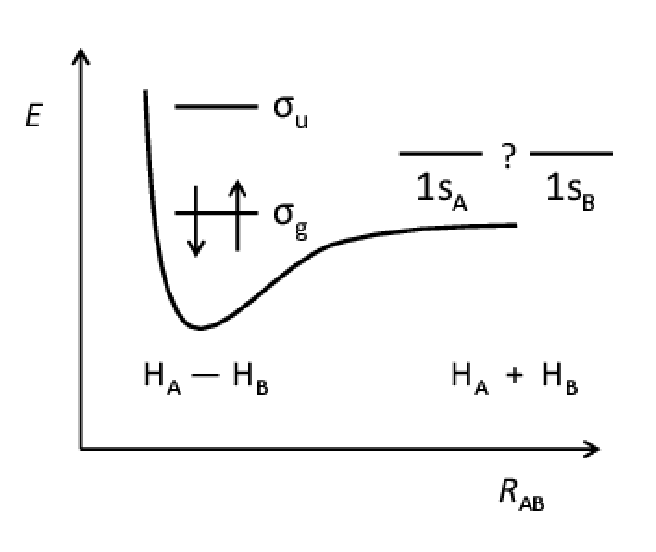
\includegraphics[scale=1]{multirefH2.eps}
\caption[Disociace molekuly vodíku]{Schematická disociační křivka molekuly vodíku a energetika molekulových a atomových orbitalů pro vázanou molekulu a disociované atomy.}
\label{obr:abinitio:multirefH2}
\end{figure}

Jenomže pro disociovanou strukturu (což je v~tomto  případě triviálně řešitelný problém metodou separace proměnných s~řešením $1s_A(1)1s_B(2)$ a $E=2E_H=-27,2\,eV$) teď nevíme, jaký orbital vlastně dosadit do Slaterova determinantu \ref{rov:abinitio:SDH2}. Vazebný nebo antivazebný? Vždyť mají oba stejnou energii. Pokud si vybereme stejně jako v~předchozím případě symetrický $\sigma_g$, získáme vlnovou funkci (pro jednoduchost zde neuvádíme spinovou část)
\begin{equation}
1s_A(1)1s_B(2)+1s_B(1)1s_A(2)+1s_A(1)1s_A(2)+ 1s_B(1)1s_B(2) .
\end{equation}
První dva členy zde odpovídají (správně) kovalentní struktuře, ale druhé dva členy popisují ionty, H$^+\cdots$H$^-$ a H$-\cdots$H$^+$. Tomu bude odpovídat energie, která bude z~poloviny dána neutrálními atomy a z~poloviny ionty. Iontové příspěvky ale nechceme, odpovídají totiž vyšší energii.
To lze lehce nahlédnout, v iontové konfiguraci totiž jsou dva elektrony u jednoho atomu a budou se tudíž odpuzovat, zatímco u dvou nekonečně vzdálených atomů vodíku se elektrony vůbec nepotkají.
Správná vlnová funkce je dána rozvojem
\begin{equation}
\psi= \sqrt{\frac{1}{2}} (\sigma_g-\sigma_u).
\end{equation}

Je tedy vidět, že v~případě rozštěpení chemické vazby za vzniku bi-radikálové struktury je potřeba použít více než jeden Slaterův determinant. Metoda HF kvalitativně selhává. Řešením je použít velmi omezený rozvoj typu konfigurační interakce, do kterého zahrneme pouze excitace z~orbitalů v~blízkosti nejvyššího obsazeného molekulového orbitalu HOMO (z~angl. \textit{Highest Occupied Molecular Orbital}) a z~nejnižšího neobsazeného molekulového orbitalu LUMO (a angl. \textit{Lowest Unoccupied Molecular Orbital}). Tuto množinu orbitalů, ze kterých a do kterých excitujeme, nazýváme aktivním prostorem. Tato metoda má zkratku CASSCF (z~angl. \textit{Complete Active Space-Self Consistent Field}). Narozdíl od metody CI u~CASSCF metody optimalizujeme obě sady koeficientů $C$ a $c_{ij}$ zároveň. 

Metoda CASSCF pokrývá tu část korelační energie, která souvisí s~principiální nedostatečností jednoho Slaterova determinantu pro popis molekuly, mluvíme o~tzv. \textbf{statické korelaci}. I~v~metodě CASSCF s~konečným aktivním prostorem je ale nesprávně popsána okamžitá interakce mezi elektrony, tj. tzv. dynamická korelace.\footnote{Dělení korelační energie na statickou a dynamickou je poněkud umělé a nelze jednoznačně definovat.} Dynamickou korelaci pak můžeme dodat kupříkladu pomocí poruchové teorie aplikované na referenční vlnovou funkci z~metody CASSCF (v~případě poruchové teorie druhého řádu pak dostaneme často užívanou metodu CASPT2), nebo pomocí metody konfigurační interakce (zde dostaneme metodu multireferenční konfigurační interakce, MRCI). Obecně mluvíme o~multi-referenčních metodách.

Disociace vazby za vzniku biradikálů není ale jediná situace, pro kterou je metoda HF nedostatečná. Jiným takovým případem jsou excitované stavy molekul. I~kdyby byl základní a excitovaný stav popsán kvalitně jedním Slaterovým determinantem, půjde o~jiný Slaterův determinant pro každý ze stavů. Pro konzistentní popis obou stavů najednou (třeba při výpočtech excitačních energií) je tudíž žádoucí opět použít rozvoj do více Slaterových determinantů. S~multireferenčními metodami se proto často setkáme ve spektroskopii a fotochemii. 

\clearpage
\section{Metody funkcionálu hustoty}
\label{sec:dft}
Pomocí metod založených na teorii funkcionálu hustoty (dále jen DFT metod) se v posledních zhruba dvaceti let provádí většina výpočtů elektronové struktury. Popularita DFT metod je dána jejich přijatelnou výpočetní náročností, která o mnoho nepřevyšuje Hartreeho-Fockovu 
metodu. Výpočty jsou ale typicky daleko přesnější, neboť DFT metody zahrnují korelační energii. Efektivita DFT je dána tím, že nepracuje s poměrně složitou vlnovou funkcí (tj. funkcí 3N souřadnic elektronů), ale s tzv. elektronovou hustotou, což je funkce pouze tří prostorových souřadnic. 

Představme si základní pojmy. Začněme pojmem \textbf{funkcionál}. Pojďme si nejprve připomenout, jak funguje funkce. Do funkce vložíme nezávislé proměnou, tedy nějaké číslo, a na oplátku dostaneme číslo jiné, neboli závisle proměnnou. Jde tedy o zobrazení z prostoru  (kupř. reálných) čísel opět do prostoru reálných čísel. U funkcionálu je to velmi podobné, akorát na vstupu není číslo, ale funkce. Pokud to tedy řekneme více matematicky, funkcionál je zobrazení z prostoru funkcí na prostor (kupř. reálných) čísel.

Takovým jednoduchým funkcionálem je určitý integrál
$$
F[f(x)] = \int_a^b f(x) \mathrm{d}x, 
$$
Určitý integrál potřebuje dodat vstupní funkci a po jeho vyčíslení dostaneme jedno jediné číslo. Povšimněte si zde zápisu funkcionálu pomocí hranatých závorek.  
Pro složitější příklad funkcionálu nemusíme chodit daleko, stačí se podívat, jak vypadá funkcionál energie v kvantové mechanice.
$$
E[\psi] = \int \psi^*\hat{H}\psi \mathrm{d}\tau .
\label{rov:dft:efunkc}
$$
S některými funkcionály jsme se tak již setkali.

Mezi funkcemi a funkcionály existují i další podobnosti. Pojmy jako minimum a maximum funkcionálu mají prakticky stejný význam. Existuje i funkcionální analogie k dobře známé derivaci funkce --- mluvíme o \textbf{variaci funkcionálu}.
Když děláme derivaci funkce, tak se vlastně díváme, co se děje se závisle proměnnou, když trochu změníme nezávisle proměnnou.
U variace je to podobné. Zajímá nás, jak se změní hodnota funkcionálu, když mírně změníme naši funkci. Přesná definice je složitější a neuvádíme ji zde. Bude ale pro nás důležité, že pro variace platí podobné vztahy, jako pro derivace. Dá se například ukázat, že v minimu funkcionálu je jeho variace nulová. Již dobře známý variační princip (konečně víme, proč se mu tak říká!) pak můžeme napsat jednoduše pomocí variace funkcionálu energie \eqref{rov:dft:efunkc} jako
$$
\delta E[\Psi] = 0 .
$$

Nyní se můžeme vrátit k definici ústřední veličiny této kapitoly --- elektronové hustoty $\rho(\mathbf{r})$.
Elektronová hustota má na rozdíl od vlnové funkce přímý fyzikální význam. Jedná se o pravděpodobnost, že v nějakém bodě prostoru najdeme \textbf{nějaký elektron}. Je důležité si uvědomit rozdíl mezi elektronovou hustotou a čtvercem vlnové funkce, který taktéž udává hustotu pravděpodobnosti. Čtverec vlnové funkce nám udává pravděpodobnost, že první elektron má spin $m_{s1}$ a je v bodě $\mathbf{r}_1$, druhý elektron má spin $m_{s2}$ a je v bodě $\mathbf{r}_2$ atd. Jedná se tedy o mnohem složitější veličinu, která závisí na celkem $4N$ proměnných, zatímco elektronová hustota závisí jen na třech proměnných.

Elektronová hustota souvisí s vlnovou funkcí systému dle vztahu
\begin{equation}
\rho=N \int |\psi(\textbf{r}_1,\textbf{r}_2,...,\textbf{r}_n)|^2 \mathrm{d}\textbf{r}_2\dots\mathrm{d}\textbf{r}_n .
\label{rov:dft:defrho}
\end{equation}
Integrujeme tedy čtverec vlnové funkce přes všechny elektrony kromě prvního. Jak již bylo řečeno, chceme pravděpodobnost najití jakéhokoli elektronu, poloha ostatních nás nezajímá, a musíme tedy přes ně prointegrovat. První elektron ale není nijak odlišný od ostatních, stejně dobře bychom ale mohli udělat to samé pro druhý elektron. Jelikož je vlnová funkce antisymetrická, došli bychom ke stejnému výsledku. Z toho vyplývá násobící faktor $N$ před integrálem.
Z této definice hned plyne několik důležitých vlastností.

\begin{itemize}
\item Elektronová hustota je nezáporná veličina, platí tedy
\begin{equation}
\rho(\mathbf{r})  > 0 .
\end{equation}
\item Pokud zintegrujeme elektronovou hustotu přes celý prostor, dostaneme počet elektronů v systému jako
\begin{equation}
\int \rho\mathrm{d}r = N
\end{equation}

\item V poloze jader má elektronová hustota maxima.
\item Pro tato maxima platí
%TOPETR: v poznamkach mas, ze to je nejaky teorem, ale neprectl jsem jaky....
\begin{equation}
\lim_{r_i \to 0} \left[ \frac{\delta}{\delta r}+2Z_A\right]\hat{\rho(r)}=0, 
\end{equation}
kde $\hat{\rho}$ je angulárně zprůměrovaná hodnota elektronové hustoty a $Z_A$ je náboj příslušného atomového jádra.
\end{itemize}

Z těchto vlastností vidíme, že pokud známe elektronovou hustotu, tak zároveň také můžeme zjistit počet elektronů, polohu jader i jejich náboj. To jsou ale přesně ty informace, které jsou potřeba ke specifikaci molekulárního hamiltoniánu
\begin{equation}
\hat{H}=\sum_{i=1}^N -\frac{1}{2}\Delta_i+\sum_{i=1}^N\sum_{j=i+1}^N\frac{1}{r_{ij}}-\sum_{i=1}^N\sum_{A=1}^K \frac{Z_A}{r_{iA}} ,
\label{rov:dft:molham}
\end{equation}
kde jsme vynechali pro jednoduchost člen popisující odpuzování jader, jenž je stejně v rámci Bornovy--Oppenheimerovy aproximace roven konstantě. Pokud ale elektronová hustota jednoznačně určuje hamiltonián, tak poté z řešení SCHR taky energii a vlnovou funkci, a tudíž všechny potřebné veličiny. Podobným způsobem se zřejmě ubíraly úvahy Hohenberga a Kohna, kteří postavili teorii DFT na pevné fyzikální základy.

\subsection{Hohenbergovy--Kohnovy teorémy}

V roce 1964 publikovali Hohenberg s Kohnem slavný článek, který odstartoval vývoj DFT metod.
V tomto článku byly dokázány dva důležité teorémy. K jejich lepšímu pochopení si ještě musíme definovat pojem \textbf{externího potenciálu} $\nu_{ext}$. Ten má pro případ hamiltoniánu \eqref{rov:dft:molham} tvar
\begin{equation}
\nu_{ext} = \sum_{i=1}^N\sum_{A=1}^K \frac{Z_A}{r_{iA}} .
\end{equation} 
Jedná se tedy o celkovou interakci elektronů s coulombickým potenciálem atomových jader. Jelikož se v DFT na vše díváme z pohledu elektronů, tak se tomu potenciálu říká externí, jelikož nepochází ze samotných elektronů. Je důležité si uvědomit, že externí potenciál vlastně definuje hamiltonián \eqref{rov:dft:molham}, neboť ostatní členy triviálně závisejí pouze na počtu elektronů v systému. Nyní již můžeme přejít ke slíbeným teorémům.

\textbf{První Hohenbergův--Kohnův teorém} hovoří o významnosti elektronové hustoty. Zní takto:

\bigskip
\noindent \uv{\textbf{Pro libovolný systém interagujících elektronů je externí potenciál $\nu_{ext}$ jednoznačně určen elektronovou hustotou} (až na konstantu)}

\bigskip
Důsledek tohoto tvrzení jsme si již naznačili dříve. Pokud máme jednoznačně daný externí potenciál, pak také známe hamiltonián a můžeme v principu spočítat vlnovou funkci i energii, které jsou tudíž jednoznačně určeny pouze elektronovou hustotou. \textbf{Elektronová energie je tedy jednoznačným funkcionálem elektronové hustoty} neboli v matematickém zápisu
\begin{equation}
E_{el}=E_{el}[\rho] .
\end{equation}
Pokud bychom tedy tento funkcionál znali a znali také správnou hustotu, tak bychom mohli získat energii i bez řešení Sch\"{o}dingerovy rovnice a hledání vlnových funkcí.

\bigskip
Pro důkaz tohoto teorému si musíme ještě odvodit pomocný vztah pro integraci externího potenciálu vynásobeného vlnovou funkcí.
Rozepišme si nejprve externí potenciál na součet jednoelektronových příspěvků:
\begin{equation}
\nu_{ext}=\sum_{i=1}^N \nu_i = \sum_{i=1}^N \sum_{A=1}^K \frac{Z_A}{r_{iA}}  
\label{rov:dft:nui}
\end{equation}
Pojďme si nyní vyčíslit integrál
\begin{equation}
\int \nu_{ext} \psi(\textbf{r}_1,...,\textbf{r}_N)^2\mathrm{d}\tau .
\end{equation}
Dosazením vztahu \eqref{rov:dft:nui} a vhodným přeuspořádáním mnohonásobného integrálu dostaneme
\begin{equation}
\sum_i^N \int \nu_i \left[\int \psi(\mathbf{r}_1,...,\mathbf{r}_N)\prod_{j\neq i}\mathrm{d}\textbf{r}_j\right] \mathrm{d}\textbf{r}_i .
\end{equation}
Výraz v hranaté závorce není ale nic jiného než elektronová hustota $\rho$ (až na násobný faktor $N$), dostáváme tedy finální vztah
\begin{equation}
\int \nu_{ext} \psi(\textbf{r}_1,...,\textbf{r}_N)^2\mathrm{d}\tau = \sum_{i=1}^N \int \nu_i(\textbf{r}_1)\frac{\rho(\textbf{r}_i)}{N}= \int \nu_i(\textbf{r})\rho(\textbf{r}) \mathrm{d}r .
\label{rov:dft:intnupsi}
\end{equation}

\bigskip 
\textbf{Důkaz HK1:} Důkaz se provádí sporem. Předpokládejme, že jedné dané hustotě $\rho$ přísluší dva různé externí potenciály $\nu_{ext1}$ a $\nu_{ext2}$, kterým přísluší hamiltoniány $\hat{H}_1$ a $\hat{H}_2$ a vlnové funkce $\psi_1$ a $\psi_2$.  Pak díky variačnímu principu musí platit

\begin{equation}
E_1 = \int \psi_1^* \hat{H}_1 \psi_1 \mathrm{d}\tau < \int \psi_2^* \hat{H}_1 \psi_2 . \mathrm{d}\tau ,
\end{equation}
protože když k hamiltoniánu $\hat{H_1}$ přiřadíme funkci $\psi_2$, která není jeho vlastní funkcí základního stavu, tak musíme dostat větší energii. Nyní chytře přepíšeme pravou stranu nerovnosti jako  
\begin{equation}
\int \psi_2^* \hat{H}_1 \psi_2 = \int \psi_2^* \hat{H}_2 \psi_2\mathrm{d}\tau  + \int \psi_2^* \left[\hat{H}_1-\hat{H}_2\right] \psi_2\mathrm{d}\tau = E_2 + \int \rho(\mathbf{r})(\nu_1-\nu_2)\mathrm{d}\mathbf{r}  
\end{equation}
V poslední rovnosti jsme využili toho, že oba hamiltoniány se liší pouze externím potenciálem, a použili jsme vztah \eqref{rov:dft:intnupsi}.

\noindent Vyšlo nám tedy, že platí nerovnost
\begin{equation}
E_1 < E_2+\int \rho(\mathbf{r})(\nu_1-\nu_2)\mathrm{d}\mathbf{r}
\label{rov:HK1_1}
\end{equation}
Tu samou argumentaci bychom ale mohli také aplikovat opačně a dostali bychom
\begin{equation}
E_2 < E_1+\int \rho(\mathbf{r})(\nu_2-\nu_1)\mathrm{d}\mathbf{r} .
\label{rov:HK1_2}
\end{equation}
Sečtením obou rovnic \eqref{rov:HK1_1} a \eqref{rov:HK1_2} tedy dostáváme
\begin{equation}
E_1 + E_2 < E_2 + E_1 ,
\end{equation}
což nemůže platit, a tedy náš původní předpoklad o existenci dvou různých externích potenciálů je také chybný.
\hfill {\footnotesize $\blacksquare$}

Formálně můžeme funkcionál energie napsat jako
\begin{equation}
E=\int \psi^*\hat{H}\psi \mathrm{d}\tau = \int \psi^*\hat{T}\psi\mathrm{d}\tau + \int \psi^*\hat{V_{el}}\psi\mathrm{d}\tau + \int \psi^*\nu_{ext}\psi\mathrm{d}\tau=\hat{T}[\rho]+\hat{V}_{ee}[\rho]+\hat{V}_{ne}[\rho] .
\end{equation}
Vidíme, že energie se stejně jako příslušný hamiltonián \eqref{rov:dft:molham} skládá ze tří různých příspěvků. Funkcionál energie tedy můžeme rozdělit na funkcionál kinetické energie elektronů $\hat{T}[\rho]$, funkcionál repulze elektronů $\hat{V}_{ee}[\rho]$ a funkcionál interakce elektronů s jádry (obecně s externím potenciálem) $\hat{V}_{ne}[\rho]$. 
Explicitní tvar posledně jmenovaného funkcionálu jsme si již vlastně odvodili rovnicí \eqref{rov:dft:intnupsi} a platí tedy
\begin{equation}
\hat{V}_{ne}[\rho] = \int \nu_i(\textbf{r})\rho(\textbf{r}) \mathrm{d}r .
\end{equation}
Součet zbylých dvou funkcionál nazýváme Hohenbergovým--Kohnovým funkcionálem a značíme $F_{HK}[\rho]$. 
Celkový funkcionál energie tedy můžeme zapsat jako
\begin{equation}
E[\rho] = \hat{T}[\rho]+\hat{V}_{ee}[\rho]+\hat{V}_{ne}[\rho] = F_{HK}[\rho] + \int \nu_i(\textbf{r})\rho(\textbf{r}) \mathrm{d}r .
\end{equation}

Přesný tvar Hohenbergova--Kohnova funkcionálu $F_{HK}[\rho]$ bohužel není dodnes znám. 
Ovšem i kdybychom jej znali, tak nám stále něco schází k jeho úspěšného použití. Nevíme totiž, jak získat pro daný systém správnou elektronovou hustotu $\rho$, kterou bychom do něj mohli dosadit. Samozřejmě kdybychom znali vlnovou funkci, tak stačí dosadit do definičního vztahu \eqref{rov:dft:defrho}. Tomu se ale právě chceme vyhnout! Smyslem celé teorie funkcionálu hustoty je vyhnout se přímému řešení elektronové SCHR.

Cestu k elektronové hustotě nám dává druhý teorém od Hohenberga a Kohna, který zní takto:

\bigskip
\textbf{Předpokládejme, že danému externímu potenciálu $\nu_{ext}$ přísluší elektronová hustota $\rho_0$. Pak pro jakoukoli jinou elektronovou hustotu\footnote{Přesněji řečeno, daná elektronová hustota musí být takzvaně $\nu$--{reprezentovatelná}, neboli musí k ní příslušet nějaký externí potenciál. Pro funkce, které toto nesplňují, 2. HK teorém neplatí.} $\rho^{\prime}$ bude platit:}
\begin{equation}
E[\rho_0] < E[\rho^{\prime}]
\label{rov:dft:HK2}
\end{equation}

Nejedná se o nic jiného než variantu variačního principu, který taky využijeme k důkazu.

\bigskip
\textbf{Důkaz:} Z prvního HK teorému plyne, že jakákoli funkce $\rho^{\prime}$ patří k externí potenciálu $\nu_{ext}^{prime}$, který je odlišný od $v_{ext}$), a přísluší k němu vlnová funkci $\psi^{prime}$. Pokud ale pro tuto vlnovou funkci vyčíslíme energii, pak nám z již známého variačního principu plyne
\begin{equation}
\int \psi^{\prime *} \hat{H} \psi^{\prime} \mathrm{d}\tau = E[\rho] > E [\rho_0],
\end{equation}
což jsme chtěli dokázat. \hfill {\footnotesize $\blacksquare$}

Druhý HK teorém nám tedy dává principiální návod, jak hledat elektronovou hustotu. Budeme hledat přes všechny možné hustoty a správná bude ta, která nám dá nejnižší energii.

Hohenbergovy--Kohnovy teorémy dávají DFT solidní fyzikální základ, moc nás ale neposunují k praktické aplikaci, jelikož neznáme přesný funkcionál $F_{HK}[\rho]$.
Praktickou cestu k DFT výpočtům ukázali až o pár let později Kohn s Shamem.

\subsection{Kohnovy--Shamovy rovnice}

Nyní stojíme před zásadním problémem najití alespoň přibližného funkcionálu $F_{HK}[\rho]$, ve kterém je zahrnuta kinetická energie elektronů, klasická Coulombická interakce mezi elektrony a dále korelační a výměnné efekty. 
%Obecně bychom chtěli spočítat co největší část energie pomocí známých dobře definovaných přibližných vztahů a zbylé části poté můžeme modelovat a odchylky poté můžeme modelovat třeba semiempiricky.(\footnote{Tento přístup by se dal přirovnat k situaci v chemické termodynamice, ve které počítáme se vzorečky platnými pro ideální chování a odchylky schováváme do aktivitních koeficientů).
Ukázalo se, že největší potíže činí dostatečně přesné vyjádření funkcionálu pro kinetickou energii.
Tento problém je tak zásadní, že budeme muset částečně obětovat náš původní cíl a vrátit se k molekulovým orbitalům.
Pokud totiž máme molekulové orbitaly, tak pomocí nich můžeme vyčíslit kinetickou energii dle vztahu
\begin{equation}
E_{kin}=\sum_{i=1}^N \int \varphi\frac{1}{2} \Delta_i \varphi \mathrm{d}\textbf{r}_i .
\end{equation}
S takto postavenou teorií přišli v roce 1965 Kohn s Shamem.

Obecná strategie odvození Kohnovy--Shamovy proceduru je následující. Definuje se fiktivní systém neinteragujících elektronů (podobně jako v Hartreeho--Fockově teorii zde elektrony interagují pouze skrze efektivní potenciál), který je zvolen tak, aby jeho elektronová hustota bylo rovna elektronové hustotě reálného systému. 
Funkcionál energie se rozepíše následujícím způsobem:
\begin{equation}
E[\rho]= T_{n}[\rho] + \frac{1}{2}\int \int \frac{\rho(\textbf{r}_1)\rho(\textbf{r}_2)}{r_{12}} + V_{nekl}(\rho) +\left[T[\rho]-T_{n}[\rho]\right] + \int \nu \rho \mathrm{d}\textbf{r},
\label{rov:dft:KSfunkc}
\end{equation}
kde $T_{n}[\rho]$ kinetická energie neinteragujícího systému, druhý člen odpovídá klasické mezi-elektronové repulzi (násobí se jednou polovinou, aby se interakce nezapočítávaly dvakrát), $V_{nekl}$ zahrnuje korelační a výměnnou energii elektronů, člen v hranaté závorce je rozdíl kinetických energií reálného a neinteragujícího systému  a poslední člen odpovídá interakci elektronů s jádry. Pokud všechny neznámé členy dáme dohromady dostaneme tzv. korelačně--výměnný potenciál
\begin{equation}	
E_{XC}[\rho]=\left[T[\rho]-T_{n}[\rho]\right] +  V_{nekl} .
\label{rov:dft:exc}
\end{equation}
% V_{ee}(\rho) - \frac{1}{2}\int \int \frac{\rho(\textbf{r}_1)\rho}{\textbf{r_{12}}}
Pokud na funkcionál \eqref{rov:dft:KSfunkc} nyní aplikujeme variační princip, tak dostaneme rovnice, které mají stejný tvar jako rovnice
pro systém neinteragujících elektronů. Jenže pro tento systém známe řešení! Stačí vyřešit vyřešit příslušnou jedno--elektronovou  	 Schr\"{o}dingerovu rovnici, velmi podobnou rovnicím Hartreeho--Focka
\begin{equation}
\left(-\frac{1}{2}\Delta_i + V_{eff} \right) \varphi_i =\epsilon_i \varphi_i ,
\label{rov:dft:KSeq}
\end{equation}
kde $V_{eff}$ je efektivní potenciál, pro který platí
\begin{equation}
V_{eff}=\nu_{ext}+\frac{1}{2}\frac{\rho(\textbf{r}^{\prime})}{|\textbf{r}-\textbf{r}^{\prime}|}\mathrm{d}\textbf{r}^{\prime}+u_{xc} ,
\end{equation}
kde $u_{xc}$ je funkcionální derivace (variace) výměnně--korelačního funkcionálu \ref{rov:dft:exc} tvar tohoto potenciálu byl odvozen tak, aby byly elektronové hustoty reálného i fiktivního systému stejné.
Rovnice \ref{rov:dft:KSeq} se nazývají Kohnovy--Shamovy a řeší se podobně jako rovnice Hartreeho--Fockovy rozvojem do báze AO.
Získáme tak sadu molekulových orbitalů, ze kterých pak dostaneme elektronovou hustotu dle vztahu (uvádíme bez důkazu)
\begin{equation}
\rho(\textbf{r}) = \sum_{i=1}^N |\varphi|_i^2
\label{rov:dft:KSrho}
\end{equation}
%Jelikož neinteragující systém byl definován tak, aby 
Tuto hustotu pak můžeme dosadit do funkcionálu \eqref{rov:dft:KSfunkc} a získáme tak požadovanou energii.

Kohn--Shamův přístup je v principu přesný, pokud bychom znali přesný tvar výměnně--korelačního funkcionálu $E_{XC}[\rho]$.
Ten sice neznáme, ale existuje spousta vztahů přibližných, o kterých pojednávají další kapitoly.


\subsection{Aproximace lokální hustoty}
Problém, který KS metoda přímo neřeší je nalezení tvaru výměnně--korelačního potenciálu.
V zásadě existují dva přístupy k tomuto problému. Buď se snažíme odvodit vhodný funkcionál Exc čistě pomocí teoretických argumentů z pokročilejších partií DFT. Druhý přístup je pragmatičtější, kokrétní tvar funkcionálu může obsahovat parametry, které se určují z experimentálních dat.

Většina DFT metod rozděluje výměnně--korelační 

Existuje několik různých rodin funkcionálů, které se liší mírou přesnosti, výpočetními nároky i svým zaměřením.

\subsubsection{Aproximace lokální hustoty}
Aproximace lokální hustoty (angl. \textit{Local Density Approximation}, LDA) vychází z tzv. modelu \textbf{homogenního elektronového plynu} (HEG). Je to hypotetický fyzikální stav, kdy máme všude konstantní elektronovou hustotu, vyváženou rovnoměrným pozitivním pozadím. Tento model je pro teorii DFT velmi užitečný, neboť pro něj máme přesné výpočty. Tento model byl ale kdysi užitečný i pro chemiky, dájí se takto třeba popsat valenční elektrony v kovech (teorie elektronového plynu). Jak ale tento model použít na atomy nebo molekuly, které mají elektronovou hustotu značně nehomogenní?

Můžeme si představit, že prostor objem atomu/molekuly rozdělíme na malinké krychličky. Ve středu každé krychličky zjistíme elektronovou hustotu, kterou poté dosadíme do vztahů plynoucích z teorie HEG.
Získáme tím elektronovou energii v této malé krychličce a celkovou energii získáme součtem přes všechny krychličky. Matematicky rigorózně to můžeme zapsat pomocí trojného integrálu přes celý prostor
\begin{equation}
E_{XC}^{LDA}[\rho]=\int \rho(\textbf{r}) \varepsilon(\rho(\textbf{r})) \mathrm{d}\textbf{r} ,
\end{equation}
kde $\varepsilon(\rho(\textbf{r}))$ je výměnně--korelační energie HEG o hustotě $\rho$ vztažená na jeden elektron. Tato rovnice definuje výše zmíněnou aproximaci lokální hustoty.

Jaký je konkrétní tvar $\varepsilon(\rho(\textbf{r}))$? Nejprve jej rozdělíme na korelační a výměnnou část (takto to dělá většina DFT metod)
\begin{equation}
\varepsilon(\rho(\textbf{r}))=\varepsilon_x(\rho)+\varepsilon_c(\rho) .
\end{equation}

\noindent Pro výměnnou část se dá odvodit následující analytický vztah
\begin{equation}
V_x[\rho]=-\frac{3}{4}\left((\frac{3}{\pi}\right)^{\frac{1}{3}}\rho^{\frac{1}{3}}
\end{equation}
Tento vztah je spojen s jménem Slater\footnote{Ano, je ten ten samý pan Slater, podle kterého jsou pojmenované naše oblíbené determinanty.}, označuje se tedy zkratkou S.

Pro korelační energii HEG nelze získat analytický výraz. Příslušné výpočty lze ale provést numericky a výsledek poté nafitovat. Výsledný korelační funkcionál je znám jako VWN (dle pánů Vosko--Wilk--Nusair). V kombinaci se Slaterovým výrazem pro výměnnou část získáme metodu SVWN (výměnná část se ve zkratce uvádí vždy první).

Mírným vylepšením je metoda spinově závislé aproximace lokální hustoty (angl. \textit{Local Spin Density Approximation}, LSDA), které pracují zvlášť s elektronovou hustotou elektronů se spinem $\alpha$ a zvlášť se spinem $\beta$.

Metoda LDA byla prvním větším úspěchem DFT teorie. Její výsledky jsou typicky typicky o něco lepší než metoda Hartreeho--Focka a můžeme ji s úspěchem použít pro stanovení geometrii, vybračních frekvencí nebo dipólových momentů. Na druhou stranu funguje méně dobře co se týče chemických reakcí. Dnes se metoda LDA používá zřídka, nahradily ji pokročilejší metody.

\subsection{GGA funkcionály}
Jednou z nevýhod DFT je absence jasné cesty k přesnějším výsledku, neboť neznáme tvar výměnně--korelačního členu, narozdíl od \textit{ab initio} metod, kde jasně víme, jak alespoň v principu dospět k přesnému výsledku (např. metodou Full CI ve velké bázi).

Jednou z možností postupu, která se nám po předchozí kapitole nabízí, je zkusit vyjít z aproximace lokální hustoty a tu se snažit dále vylepšit. V LDA je v daném bodě využívali pouze hodnotu elektronové hustoty. Taylorův rozvoj nám napovídá, že by mohlo být užitečné využít informaci o \textbf{gradientu hustoty} $\nabla\rho(\textbf{r})$. 
Tím se dostaneme k metodám \textbf{generalizovaného gradientu} (z angl. \textit{Generalized Gradient Approximation}, GGA), pro které má výměnně--korelační funkcionál obecný tvar
\begin{equation}
E_{xc}^{GGA}=\int \rho(\textbf{r})f(\rho,\Delta\rho) \mathrm{d}\textbf{r} .
\end{equation}
Konkrétní tvar těchto funkcionálů již bývá značně složitý a často obsahuje nastavitelné parametry. Mezi nejznámější výměnné GGA funkcionály patří například Beckeho výměnný funkcionál (zkratka \textbf{B88}, nebo jen B), který obsahuje jeden parametr. Mezi známé korelační funkcionály patříl například \textbf{LYP} (od pánů Lee, Yang a Paara) nebo \textbf{P86} (autor Perdew). Jejich kombinací pak získáme známe často užívané metody \textbf{BP86} a \textbf{BLYP}. Dalším výměnně--korelačním funkcionálem je \textbf{PBE}(Perdew, Burke, Erzenhof), který neobsahuje žádné parametry.

GGA funkcionály jsou značně přesnější než LDA, a proto právě tyto funkcionály odstartovaly masové používání DFT v kvantové chemii.

Dalším logickým krokem ke zlepšení je využití dalších informací kromě gradientu, například druhé derivace. Mluvíme potom o meta-GGA funkcionálech, mezi které patří například korelační funkcionál B95 nebo výměnně--korelační funkcionál TPSS.

\subsection{Hybridní funkcionály}
Pozorný čtenář by se mohl ptát, proč vlastně k výpočtu výměnné energie nevyužijeme Kohn--Shamovy orbitaly, když je konec konců používáme pro výpočet kinetické energie. Využily bychom vzoreček známý z HF teorie 
\begin{equation}
E_X^{exact}=-\frac{1}{2}\sum_{i=1}^N\sum_{j=1}^N K_{ij} . 
\end{equation}
Bohužel se ukázalo, že použití tohoto vzorce (spolu s nějakým korelačním funkcionálem) nevede k dobrým výsledkům, jelikož se tím naruší delikátní kompenzace chyb v současných funkcionálech.

Tím dostaneme takzvané hybridní funkcionály, které představují další výrazné zlepšení přesnosti.
Mezi hybridní funkcionály patří i funkcionál \textbf{B3LYP}, který je v současnosti suverénně nejpoužívanější kvantově--chemickou metodou (přestože byl vyvinut už v roce 1993)
Jeho přesný tvar je
\begin{equation}
E_{xc}^{B3LYP}=(1-a_0-a_x)E_x^{LDA}+a_0E_x^{exact}+a_xE_x^{B88}+(1-a_c)E_c^{VWN}+a_c E_c^{LYP}
\end{equation}
a nastavitelné parametry mají hodnotu $a_0=0,2$, $a_x=0,72$ a $a_c=0,81$.
Parametr $a_0$ určuje procento přesné výměnné energie; B3LYP má tedy 20\% podíl HF výměnné energie.

Z dalších mnoha hybridních funkcionálů uveďme alespoň (v závorkách úvádíme procento HF výměnné energie): PBE0 (25\,\%), BMK (50,BHandHLYP(50\,\%)

\subsubsection{Moderní funkcionály}
Oblast DFT metod je jednou z nejbouřlivěji vyvíjejících se částí kvantové chemie. V současnosti už existují stovky různých funkcionálů. V posledních letech se objevilo mnoho různých nových typů kromě výše zmíněných. Pro výpočet excitovaných stavů se například hodí takzvané \textit{range--separated funkcionály}. 
%Mělo by platit, že $lim_{V_x\to \infty}=\frac{1}{r}$
%zmínka o self-interakční chybě.

Pro výpočet slabých mezimolekulových interakcí existují speciální empirické korekce.

I přes své stáří však pro rutinní výpočty stále dominuje funkcionál B3LYP díky jeho velké univerzalitě a přesnosti.
Pro detailní přehled starších i moderních funkcionálů lze nahlédnout do návodu k programu Gaussian\footnote{\textit{http://www.gaussian.com/g\_ tech/g\_ ur/k\_ dft.htm}}.


%\textbf{Disperzní korekce}

%Grimmeho empirická korekce
%\begin{equation}
%E_{vdw}=-s_6\sum c^{ij}r_{ij}^{-6}
%\end{equation}
%Koeficient $s_6$ závisí na použitém funkcionálu, zatímco koeficienty $c_{ij}$ závisí na typu interagujících atomů.

%\textbf{Dvojitě hybridní funkcionály}
%S.Grimme 
%\begin{equation}
%E_{xc}^{hybrid}=a_1E_x^{GGA}+(1-a_1)E_x^{EXACT}+a_2E_c^{GGA}
%\end{equation}
%Pro tento tvar se vyřeší KS rovnice a získají KS orbitaly. Z těchto orbitalů se poté vypočítá MP2 korekce
%ze vzorečku XX a přídá se k $E_{xc}^{hybrid}$

%\begin{equation}
%E_{xc}^{DH}=E_{xc}^{hybrid}+(1-a_2)E_c^{KS-MP2}
%\end{equation}

%Příkladem může být B2LYP s parametry $a_1=0,47$ a $a_2$=0,73

%\textbf{Jakobův žebřík, obrázek (Genesis 28:10-12)}


\clearpage
\section{Semiempirické přístupy}
\label{kap:semiemp}
V této kapitole se podíváme na skupinu semiempirických metod. Ačkoli semiempirické metody také vycházejí z řešení elektronové Schr\"{o}dingerovy rovnice (odtud přízvisko \textit{semi}), jejich rovnice obsahují dodatečné parametry, jejichž hodnoty se typicky získávají z přesnějších \textit{ab initio} výpočtů nebo se z experimentálních dat (odtud \textit{empirické}).

Aproximace, které tyto metody využívají, můžeme rozdělit do dvou skupin. V první řadě, většina semiempirických metod nevychází z přesného molekulárního hamiltoniánu XX, ale určitého efektivního hamiltoniánu, ve kterém jsou zanedbány některé členy. Většina semiempirických metod se například soustředí pouze na valenční elektrony (příspěvek ostatních elektronů je brán jako konstanta), což celkový hamiltonián systému značně zjednoduší.

Po určení hamiltoniánu se při odvození typické semiempirické metody postupuje obdobně jako při odvození HF rovnic. Zvolíme si konkrétní tvar vlnové funkce a zvolíme bázi (metoda MO-LCAO) a aplikací variačního principu odvodíme pracovní rovnice. V tomto kroku ale u semiempirických metod dojde k dalšímu zjednodušení. Buď můžeme některé členy z rovnic úplně zanedbat a položit rovno nule, anebo je můžeme považovat za konstantu, jejíž hodnotu určíme tak, aby nám to vycházelo.   

Motivací k vývoji semiempirických metod bylo zmenšení výpočetních nároků \textit{ab initio} metod s pokud možno co nejmenším ovlivněním přesnosti. Nicméně i metody, které byly kvantitativně nepřesné, se ukázaly jako velmi užitečné, neboť dovolily kvalitativní pochopení zákonitostí chemických vazeb a jiných vlastností molekul. Na jednu takovou metodu, která nám dala známé pravidlo \uv{$ 4n+2 $} pro určení aromaticity, se nyní podíváme.

\subsection{H\"{u}ckelova metoda}

H\"{u}ckelova metoda (dále jen HM) je historicky první a asi i nejjednoduší semiempirická metoda. Pro rozumné molekuly je pro použití této metody potřeba doslova jen tužka a papír. Její jednoduchost spočívá v tom, že se soustředí pouze na $\pi$ vazebné elektrony,
tedy elektrony v molekulových orbitalech složených z atomových \textit{p} orbitalů.
Její použití je tudíž omezeno na planární systémy s vícenásobnými vazbami. 

Hamiltonián HM metody má následující tvar:
\begin{equation}
H_{HMO}= \sum h_{i, eff}^\pi
\label{rov:Ham_HM}
\end{equation}
kde $h_{i, eff}^\pi$ je jednoelektronový potencál $\pi$ elektronu, který v sobě obsahuje jak kinetickou energii, tak interakce s ostatními elektrony.
Z toho zřejmé, že elektrony jsou považovány za nezávislé. (to je zásadní rozdíl oproti metodě HF, ve které je nezávislost elektronů vyjádřena \uv{pouze} tvarem vlnové funkce). 
Konkrétní tvar těchto efektivních elektronových hamiltoniánů není specifikován a bere se pouze jako parametr metody. 

Dalším krokem je výběr báze. V případě metody HM to budou $p_z$ orbitaly všech uhlíkových atomů.
\begin{equation}
\psi= \sum_i c_i \phi_i
\end{equation}
Tím převedeme problém najití vlnové funkce na jednodušší problém najití koeficientů $c_i$. Pokud tuto vlnovou funkci dosadíme do SCHR s Hamiltoniánem \ref{Ham_HM} a aplikujeme variační princip, dostaneme sadu sekulárních rovnic. Z nich poté obdržíme sekulární determinant:
\begin{equation}
|\mathbf{H}-\epsilon \mathbb{S}|=0
\label{rov:HM_det}
\end{equation}

Pro lepší ilustraci budeme nadále uvažovat výpočet pro molekulu butadienu.
Naše báze se tedy bude skládat ze čtyř $p_z$ orbitalů.

Aplikací variačního principu poté dostaneme následující sekulární rovnice:
\begin{equation}
\begin{vmatrix}
H_{11}-\epsilon S_{11} & H_{21}-\epsilon S_{21} & H_{31}-\epsilon S_{31} & H_{41}-\epsilon S_{41}  \\
H_{12}-\epsilon S_{12} & H_{22}-\epsilon S_{22} & H_{32}-\epsilon S_{32} & H_{42}-\epsilon S_{42}  \\
H_{11}-\epsilon S_{13} & H_{23}-\epsilon S_{23} & H_{33}-\epsilon S_{33} & H_{43}-\epsilon S_{43}  \\
H_{11}-\epsilon S_{14} & H_{24}-\epsilon S_{24} & H_{34}-\epsilon S_{34} & H_{44}-\epsilon S_{44}
\end{vmatrix}
= 0
\end{equation}
Nyní bychom měli spočítat integrály $H_{ij}$ a $S_{ij}$, které v principu závisí na geometrii systému.
V rámci H\"{u}ckelovy aproximace na ně ale pohlížíme jako na parametry metody
a naložíme s nimi takto:
\begin{itemize}
\item zanedbáme překryvové integrály mezi AO na různých atomech tj. $S_{ij}=\delta_{ij}$;
\item integrály $H_{ii}=\alpha$ těmto integrálům říkáme coulombovské integrály
\item integrály $H_{ij}$ položíme rovno nule, pokud orbitaly nepatří sousedním atomům.
Nenulové integrály položíme rovno parametru $\beta$ a nazýváme je rezonančními integrály.
\end{itemize}

Takto zjednodušené rovnice poté vyřešíme. Nejprve najdeme vlastní čísla přes sekulární determinant a následně určíme koeficienty $c_i$. V případě butadienu bude sekulární determinant vypadat následovně:
\begin{equation}
\begin{vmatrix}
\alpha-\epsilon & \beta & 0 & 0  \\
\beta &\alpha-\epsilon & \beta & 0  \\
0 &\beta &\alpha-\epsilon & \beta  \\
0 & 0 & \beta &\alpha-\epsilon  
\end{vmatrix}
= 0
\end{equation}
%Tento determinant vede na rovnici čtvrtého stupně, kterou lze ale vhodnou substitucí řešit analyticky.
Ve druhém kroku jsme determinant vydělily $\beta$ a zavedli substituci $x=\frac{\alpha-\beta}{\epsilon}$.
Nyní rozvojem determinantu podle prvního řádku dostaneme:
\begin{equation}
x
\begin{vmatrix}
x & 1 & 0 \\
1 & x & 1 \\
0 & 1 & x \\
\end{vmatrix}
-
\begin{vmatrix}
x & 1 & 0 \\
1 & x & 1 \\
0 & 1 & x \\
\end{vmatrix}
=x^4-3x^2+1=0
\end{equation}
Tuto kvartickou rovnici můžeme naštěstí převést na kvadratickou pomocí substituce $y=x^2$ a dostaneme:
\begin{equation}
y^2-3y+1=0; y_1=2,62 a y_2=0.382
\end{equation}
a tedy
\begin{equation}
x_{1,2}=1,62
x_{3,4}=0,62
\end{equation}
Z toho vyplývají násůedující hodnoty energií:
$$ \epsilon_1 = \alpha+1,62\beta $$
$$ \epsilon_2 = \alpha+0,62\beta $$
$$ \epsilon_3 = \alpha-0,62\beta $$
$$ \epsilon_4 = \alpha-1,62\beta $$
Zpětným dosazením do sekulárních rovnic bychom poté dopočítali koeficienty $c_i$.
Jak nyní získáme parametry?...

\textbf{Spektroskopie}
Jak můžeme pomocí HM spočítat excitační energii? Prostě formálně excitujeme jeden elektron z obsazeného do neobsazeného orbitalu a potom spočítáme celkovou energii a od ní odečteme celkovou energii zákaldního stavu. Pokud budeme chtít spočítat nejnižší excitační energii butadienu, přesuneme jeden elektron z orbitalu 3 do orbitalu 2. Výsledná energie potom bude:
$$
\Delta E = \epsilon_3-\epsilon_4 = 1,24 \beta = \frac{hc}{\nu} 
$$
Vlnová délka excitujícího záření potom vyjde 287\,nm, zatímco experimentální hodnota je kolem 200\,nm.
Soulad to není ideální, ale není ani tragický, na to že jsme jej získali tak jednoduše. HM také správně zachycuje experimentální fakt, že excitační energie se snižuje se zvyšující se délkou řetězce obsahující konjugované dvojné vazby.

\textbf{Delokalizační energie}

$$
\left| \right|=0
$$
z čehož nám vyjde
$$
(\alpha-\epsilon)^2=\beta^2
$$
$$
\alpha - \epsilon = \pm \beta
\epsilon_{1,2}= \alpha\pm \beta
$$
Pro butadien poté vyjde delokalizační energie $E_D=0,472\beta=35,4 kJ/mol$
Experimentálně můžeme míru delokalizace určit pomocí hydrogenačních tepel a opět to vztáhnout vůči ethanu.
Hydrogenační teplo ethanu (tj. entalpie reakce ethan + H$_2$ = ethen) je -136,94\,kJ/mol, zatímco hydrogenační teplo butadienu je -240\,kJ/mol. Experimentální delokalizační energie je tedy:
$$
E_D^{exp}=2\cdot139,9-240 = 33,8 kJ/mol,
$$
což je v dobrém souladu s námi vypočtenou hodnotou.

\textbf{Cyklické systémy a aromaticita}
Asi největším úspěchem HM bylo vysvětlení aromaticity cyklických molekul.
Například pro benzen dává HM následující strukturu molekulových orbitalů:
Pokud bychom nyní zkoušeli počítat delokalizační energii pro různý počet elektronů, zjistili bychom, že má maximum pro šest elektronů, tedy pokud plně zaplníme všechny vazebné orbitaly.

Pokud bychom spočítali HM metodou obecně pro cyklické uhlovodíky, došli bychom ke známému H\"{u}ckelovu pravidlu $4n+2$. Z diagramu pro benzen je patrnén, že pro 4n+1 elektronů bychom měli radikál, zatímco pro $4n$ elektronů bychom měli dokonce biradikál.

\begin{priklad}
\textbf{Zadání:} Jak to bude s aromaticitou cyklopropenylového radikálu? A co cyklopentadienylový radikál?

\textbf{Reseni:} V cyklopropenylu máme tři elektrony v $p_z$ orbitalech, stabilnější tedy bude cyklopropenylový kation. Podobně tomu je u cyklopentadienylu máme elektronů pět, stabilnější bude cyklopendienylový anion, který se opravdu často vyskytuje jako ligand v komplexech kovů.
\end{priklad}

\textbf{obrazek}
\bigskip

\subsection{Rozšířená H\"{u}ckelova metoda}

\begin{itemize}
\item Počítá i se $\sigma$ vazbami
\item $H_{ii}=-I_i$
\item $H_{ij}=\frac{1}{2}K(I_i+I_j)S_{ij}$
\item Dá se použít pro hledání geometrie
\item Podobně jako v původní H\"{u}ckelově metodě tvar pracovních rovnic nezávisí na řešení, a tudíž není třeba iterovat. Rozšířená H\"{u}ckelova metoda se proto i nyní rutinně využívá v kvantově chemických programech k prvotním nástřelu vlnové funkce.
\end{itemize}


\subsection{Moderní semiempirické metody}

 Vycházíme z HF, ale zanedbáváme některé 2-elektronové integrály
 Pár vět o CNDO (Complete Neglect of Differential Overlap),
 INDO (Intermediate Neglect of Differential Overlap),
 MINDO (Modified Neglect of Differential Overlap)
 AM1(Austin model 1), PM6 atp.

Ačkoli jsou semiempirické zjednodušením původních HF rovnic, často poskytují řešení lepší než HF.
To je dáno tím, že parametry jsou fitovány na experimentální data, a mohou tedy implicitně zahrnout část korelační energie.


 

\clearpage
\section{Molekulární vlastnosti}
Experimentálně molekuly charakterizujeme pomocí nejrůznějších vlastností: můžeme změřit třeba NMR posuny, elektrické či magnetické parametry či třeba jejich optickou otáčivost. Tyto molekulární vlastnosti musí být v~principu možné vypočítat metodami kvantové chemie. V~duchu axiomatiky kvantové teorie musí být přitom všechny vlastnosti molekul nějakým způsobem získatelné z~vlnové funkce. V~našich úvahách jsme se doteď soustředili na jednu konkrétní veličinu, na energii. Tu vypočítáme přímo ze Schr\"odingerovy rovnice $\hat{H} \psi = E \psi$ snadno jako

\begin{equation}
E = \int \psi^{\ast} \hat{H} \psi \mathrm{d} \tau.
\label{rov:Vl-1}
\end{equation}

Energie je veličina prvořadé důležitosti, představuje klíč ke struktuře molekul, termodynamice chemických reakcí či k~celé spektroskopii. Mohou nás ale ale zajímat libovolné jiné veličiny, například obecně veličina A, které přísluší operátor $\hat{A}$. Střední naměřená hodnota této veličiny je pak dána jako

\begin{equation}
\braket{A} = \int \psi^{\ast} \hat{A} \psi \mathrm{d} \tau.
\label{rov:Vl-2}
\end{equation}

V~této krátké kapitole se podíváme na některé molekulární vlastnosti.

  
\subsection{Elektrické vlastnosti molekul}
Na nabité částice silově působí elektrické pole. Uvažme nyní neutrální molekulu. V~ní je nějakým způsobem rozložený náboj, toto rozložení náboje v~prostoru je dáno elektronovou hustotou $\rho(\vec{r})$ a náboji jednotlivých jader $q_I=Z_I e$. Sečteme-li celkovou hustotu náboje přes celý prostor, dostaneme pro neutrální molekulu nulovou hodnotu. I~na neutrální molekulu ale vnější elektrické pole působí, neboť náboj v~ní není rozložen rovnoměrně. Tak v~molekule HCl je o~něco více elektronové hustoty soustředěno kolem atomu chlóru než kolem atomu vodíku a~z~elektrického hlediska pak na molekulu chlorovodíku můžeme pohlížet jako na soustavu

\begin{equation}
\delta+ \dots \delta- \nonumber
\end{equation}
ve vzdálenosti $r$. Říkáme, že molekula HCl má nenulový \textbf{dipólový moment} daný v~tomto případě vztahem

\begin{equation}
\vec{\mu} = q \cdot r,
\label{rov:Vl-3}
\end{equation}

\noindent kde $q$ je náboj a $r$ je vzdálenost mezi náboji. 

Jak bychom mohli dipólový moment molekuly vypočítat? Uvažme jakoukoliv molekulu v~určitém geometrii (tj. s~určitými polohami atomových jader). V~této molekule se pohybují elektrony, každý z~nich má okamžitou polohu $\vec{r}$. Okamžitá hodnota vektoru dipólového momentu pro dané uspořádání elektronů je dáno jako

\begin{equation}
\vec{\mu} = - \sum_{i=1}^{N_{el}} e \cdot \vec{r_i} + \sum_{I=1}^{N_{jad}} e Z_I \vec{R_I},
\label{rov:Vl-4}
\end{equation}

\noindent kde $e$ je elementární náboj elektronu, $\vec{r}_i$ je poloha i-tého elektronu, $Z_I$ je nábojové číslo $I$-tého atomového jádra a $\vec{R}_I$ je poloha $I$-tého atomového jádra. Chceme-li nyní získat dipólový moment molekuly, musíme hodnotu dipólového momentu pro danou konfiguraci váhovat pravděpodobností, že daná konfigurace nastane. Jinými slovy, musíme vypočítat střední hodnotu dipólového momentu

\begin{equation}
\braket{\vec{\mu}} = \int \vert \psi_{el} \vert^2 \vec{\mu} \mathrm{d} \vec{r_1} \dots \mathrm{d} \vec{r_N} = - e \int \left( \vert \psi_{el} \vert^2 \sum_{i} \vec{r_i} \right) \mathrm{d} \vec{r_1} \dots \mathrm{d} \vec{r_N} + e \sum_{I} Z_I \vec{R_I}.
\label{rov:Vl-5}
\end{equation}

Vidíme tak, že ze znalosti vlnové funkce přímo získáme i hodnotu dipólového momentu molekuly. Stejným způsobem bychom získali třeba také kvadrupólový moment molekuly, který vykazuje například molekula oxidu uhličitého, která má jinak nulový dipólový moment. Podívejme se ještě na jinou vlastnost molekuly, na polarizovatelnost $\alpha$. Tato veličina nám říká, jak je molekula citlivá na vnější elektrické pole. V~molekula se po vložení do elektrického pole o~intenzitě $\vec{E}$ indukuje dipólový moment

\begin{equation}
\vec{u}_{ind} = \alpha \vec{E},
\label{rov:Vl-6}
\end{equation}

\noindent přičemž konstantou úměrnosti je právě polarizovatelnost $\alpha$ (tento vztah platí toliko pro malé intenzity pole). Vidíme nyní, jakým způsobem bychom polarizovatelnost mohli najít: vypočítali bychom dipólový moment molekuly v~elektrickém poli a molekuly bez elektrického pole. Rozdíl těchto dipólových momentů by po vydělení intenzitou elektrického pole poskytne hodnotu polarizovatelnosti. Sluší se dodat, že ve skutečnosti se polarizovatlenost počítá ještě jednodušeji a dvou výpočtů není potřeba. Tento detail jde však za rámec tohoto úvodního textu. Za malý komentář stojí také fakt, že polarizovatelnost představuje obecně tenzor, tj. matici a nikoliv pouhé číslo. Elektrické pole orientované například ve směru osy $z$ může totiž indukovat i dipólový moment ve směru osy $x$ či $y$. Jak je to možné? Představme si třeba elektron, jehož pohyb je omezen na pohyb po šroubovici. Elektrické pole ve směru osy šroubovice vyvolá částečně i~pohyb elektronu ve směru na šroubovici kolmý. 

Podobným způsobem jako jsme vypočítali z~elektronové vlnové funkce dipólový moment či polarizovatelnost můžeme v~principu vypočítat jakoukoliv vlastnost molekuly, od NMR či EPR parametrů, přes geometrie molekuly, jejich vodivosti či spektrální vlastnosti.  



\subsection{Parciální náboje atomů}

V~předchozím oddíle jsme prohlásili, že v~molekule HCl je na atomu chlóru parciální záporný náboj a na atomu vodíku naopak parciální kladný náboj. Dokáže kvantová chemie tyto náboje vypočítat? To je poněkud delikátnější otázka než se zdá. Na rozdíl od dipólového momentu totiž parciální náboj na atomech nepředstavuje dobře definovanou, měřitelnou veličinu. Parciální náboj nám sděluje, kolik elektronů \uv{patří} atomu chlóru. jenže to hodně záleží na tom, \uv{kam až sahá Krakonošovo}, tedy jakou část prohlásíme za příslušnou atomu chlóru a jakou část za přiléhající vodíku. Existují tudíž různé způsoby, jak parciální náboje na molekulách vypočítat. Mluvíme o~tzv. populační analýze, neboť se snažíme vypočítat populaci elektronů příslušející určitému atomu.

Nejrozšířenější metodou populační analýzy je tzv. \textbf{Mullikenova populační analýza}. Uvaž\-me vlnovou funkci v~rámci metody Hartreeho-Focka. Ta je dána jako antisymetrizovaný součin molekulových orbitalů

\begin{equation}
\psi(\vec{r_1}, \dots, \vec{r_N}) = \hat{A} \phi_1 (\vec{r_1}) \dots \phi_N (\vec{r_N}),
\label{rov:Vl-7}
\end{equation}

\noindent kde $\hat{A}$ je antisymetrizační operátor, který ze součinu molekulových orbitalů $\phi_j$ udělá Slaterův determinant. Molekulární orbital $\phi_j$ můžeme dále vyjádřit jako lineární kombinaci atomových orbitalů

\begin{equation}
\phi_j (\vec{r_j}) = \sum_r c_{jr} \chi_r (\vec{r_j}),
\label{rov:Vl-8}
\end{equation}

\noindent kde $\chi_r$ představuje atomový orbital a $c_{jr}$ představuje rozvojový koeficient, který nám říká, jak moc přispívá atomový orbital $\chi_r$ do molekulového orbitalu $\phi_j$. Z~\uv{účetních} důvodů si tento rozvoj napišme ještě pomocí jiného indexu

\begin{equation}
\phi_j (\vec{r_j}) = \sum_s c_{js} \chi_s (\vec{r_j}).
\label{rov:Vl-9}
\end{equation}

Trik Mullikenova přístupu spočívá v~tom, že u~atomových orbitalů víme, jakému atomu přísluší. Můžeme proto sečíst příspěvky jednotlivých atomových orbitalů do celkové vlnové funkce a tím zjistit, jak moc do vlnové funkce přispívá určitý atom. Celkový počet elektronů $N$ můžeme napsat jako

\begin{eqnarray}
N &=& \sum_{j=1}^{n} \int \phi_j (\vec{r_j}) \phi_j (\vec{r_j}) \mathrm{d} \vec{r_j} = \sum_{j=1}^{n} \sum_{r,s} c_{jr} c_{js} \int \chi_j (\vec{r_j}) \chi_s (\vec{r_j}) \mathrm{d} \vec{r_j} \nonumber \\
&=& \sum_{j=1}^{n} \left( \sum_r c_{jr}^2 + \sum_{r \not = s} c_{jr} c_{js} S_{rs} \right).
\label{rov:Vl-10}
\end{eqnarray}

\noindent kde $S_{rs}$ je překryvový integrál mezi atomovými orbitaly $\chi_r$ a $\chi_s$. Tuto rovnici můžeme rozepsat jako příspěvky členů pocházejících od jednotlivých atomů $k$

\begin{equation}
N = \sum_k N_k
\label{rov:Vl-11}
\end{equation}

\noindent kde

\begin{equation}
N_k = \sum_{j=1}^{n} \left( \sum_{r \in k} c_{jr}^2 + \sum_{r,s \in k; r \not s} c_{jr} c_{js} S_{rs} + \frac{1}{2} \sum_{r \in k, s \not \in k} c_{jr} c_{js} S_{rs} \right),
\label{rov:Vl-12}
\end{equation}

\noindent V~posledním členu rovnice \eqref{rov:Vl-12} se mísí příspěvky od atomu $k$~a od některého jiného z~atomů, tento příspěvek v~Mullikenově přístupu rozdělíme rovnoměrně mezi oba atomy. Veličina $N_k$ představuje elektronovou populaci na daném atomu. Parciální náboj $q_k$ pak získáme jako rozdíl nábojového čísla atomového jádra $Z_k$ a elektronové populace $N_k$

\begin{equation}
q_k = Z_k - N_k.
\label{rov:Vl-13}
\end{equation}


\begin{priklad}
Mullikenovu populační analýzu můžeme snadno provést v~rámci H\"uckelovy metody. Zde je situace obzvláště jednoduchá, neboť překryvové integrály $S_{rs}=0$. Vlnové funkce dvou nejvyšších obsazených stavů v~molekule butadienu jsou dány jako

\begin{eqnarray*}
\phi_1 &=& 0{,}37 \chi_1 + 0{,}60 \chi_2 + 0{,}60 \chi_3 + 0{,}37 \chi_4\\
\phi_2 &=& 0{,}60 \chi_1 + 0{,}37 \chi_2 - 0{,}37 \chi_3 - 0{,}60 \chi_4
\end{eqnarray*}
 
\noindent kde $\chi_1,\chi_2, \chi_3$ a $\chi_4$ představuje 2p$_Z$ orbitaly jednotlivých atomů uhlíku. Vztah \eqref{rov:Vl-11} se zde mění na jednoduchou formuli

\begin{equation}
N_k = \sum_j n_j c_{jk}^2, \nonumber
\end{equation}

\noindent kde $n_j$ je obsazovací číslo $j$-tého molekulového orbitalu a $c_{jk}$ je příslušný rozvojový koeficient. Elektronová populace na prvním atomu uhlíku je dána jako

\begin{equation}
N_1 = 2 \cdot 0{,}37^2 + 2 \cdot 0{,}60^2 = 1 \nonumber
\end{equation}


\noindent a podobně pro ostatní atomy

\begin{eqnarray*}
N_2 &=& 2 \cdot 0{,}60^2 + 2 \cdot 0{,}37^2 = 1, \\
N_3 &=& 2 \cdot 0{,}60^2 + 2 \cdot (-0{,}37)^2 = 1, \\
N_4 &=& 2 \cdot 0{,}37^2 + 2 \cdot (-0{,}60)^2 = 1,
\end{eqnarray*}

Vidíme tedy, že všechny atomy mají $\pi$ elektronovou populaci stejnou, čtyři $\pi$ elektrony se rovnoměrně rozdělily mezi atomy. To není moc zajímavý výsledek, ale pojďme vlnovou funkci analyzovat dále. Definujme si řád vazby jako


\begin{equation}
P_{kl} = \sum_j n_j c_{jk} c_{jl}.
\label{rov:Vl-14}
\end{equation}

\noindent Pak vidíme, že $\pi$ elektronový řád vazby mezi prvním a druhým atomem uhlíku je

\begin{equation}
P_{12} = 2 \cdot 0{,}37 \cdot 0{,}60 + 2 \cdot 0{,}37 \cdot 0{,}60 = 0{,}89
\end{equation}

\noindent a mezi druhým a třetím atomem pak

\begin{equation}
P_{23} = 2 \cdot 0{,}60 \cdot 0{,}60 + 2 \cdot 0{,}37 \cdot (-0{,}37 = 0{,}44 \nonumber
\end{equation}


Celkový řád vazby (po přičtení 1 za sigma vazbu) je tak 1,89 pro vazby mezi prvním a~druhým atomem a 1,44 za vazbu mezi druhým a třetím atomem. Charakter jednotlivých vazeb je tak značně odlišný.
\end{priklad}


Mullikenova populační analýza má samozřejmě své problémy. Výrazně závisí na volbě báze. Je snadné si představit bázi, která vůbec nebude lokalizovaná na atomech. Mullikenova analýza pak poskytne nulové populace elektronů na atomech, což zjevně nedává smysl. Mullikenova analýza proto dobře funguje pro menší báze, pro větší a difúznější báze je poněkud nespolehlivá. Náboje na atomech ale můžeme vypočítat i jiným způsobem. Můžeme třeba vyžít skutečnosti, že dipólový moment fyzikální veličinou je. Můžeme pak nastavit parciální náboje takovým způsobem, abych dostali vypočítaný dipólový moment. Podobná technika založená na fitování elektrostatického potenciálu generovaného molekulou se nazývá CHElP (z~angl. \textit{Charges from Electrostatic Potential}). Tento přístup je dosti spolehlivý a v~praktickém použití jej lze doporučit.



   
         
   





      

 



\clearpage
\section{Výpočty elektronově excitovaných stavů}
Většinu chemiků zajímá dění v~základním elektronovém stavu: jaká je struktura molekul, kapalin, či krystalů, jaké jsou solvatační či mřížkové energie, jaké je rovnovážné složení reakční směsi atp. S~elektronově excitovanými stavy se nicméně chemik setká v~souvislosti s~různými spektroskopickými technikami: UV absorpční spektroskopie, rentgenová spektroskopie, spektroskopie založené na elektronovém cirkulárním dichroismu či v~nejrůznějších fluorescenčních technikách. Nesmíme přitom zapomenout ani na samostatné odvětví chemie zaměřené na chemii světla, na fotochemii. Porozumět vlastnostem elektronově excitovaných stavů je důležité v~nejrůznějších aplikacích, od biofyzikálních problémů (Jak probíhá fotosyntéza? Jakým  způsobem je přenášen zrakový vjem?) až po technologie a materiálové inženýrství (Jak fungují solární články?). 

Na první pohled se zdá, že není nutné pro excitované stavy vytvářet samostatný oddíl. Jestliže řešíme elektronovou Schr\"odingerovu rovnici

\begin{equation}
\hat{H} \psi_i = E_i \psi_i ,
\label{rov:Ex-1}
\end{equation}

\noindent získáváme tak kromě energie základního stavu $E_0$ a příslušné vlnové funkce $\psi_0$ i stavy excitované s~energiemi $E_i$, $i > 0$. Tak tomu v~principu je, nicméně je třeba mít na paměti, že většina kvantově-chemických metod, které byly doposud v~našem textu představeny, jsou designovány pro výpočty v~základním elektronovém stavu a jejich použití pro excitované stavy bez dalších úprav není možné. Příkladem mohou být metody založené na teorii funkcionálu hustoty. Hohenbergovy-Kohnovy teorémy jsou odvozeny pro elektronovou hustotu základního stavu a~rozšíření metody DFT do excitovaného stavu není vůbec samozřejmé. Při výpočtech excitovaných stavů musíme být také ostražití při volbě jednoelektronové báze. Zatímco v~základním stavu se vlnová funkce typicky příliš nevzdaluje od atomových jader, ve stavech vzbuzených může být úplně jinak.  

Příkladem metod, které je snadné rozšířit do excitovaného stavu, jsou přístupy založené na metodě konfigurační interakce. Zejména vhodné a často používané jsou multireferenční přístupy (viz kapitola \ref{kap:abinitio}). Často se tak setkáme s~metodou CASSCF a jejich poruchovým  vylepšením CASPT2 či s~vylepšením pomocí metody konfigurační interakce, metodou MRCI.   

Předpokládejme nyní, že jsme schopni vypočítat energie a vlnové funkce základního i excitovaného stavu. Mohlo by nás zajímat, kdy pak bude světlo o~frekvenci $\nu$ absorbováno či kdy naopak molekula ve vzbuzeném stavu přeskočí do stavu základního za vyzáření fotonu o~energii $h\nu$. Musí být především splněna rezonanční podmínka 


\begin{equation}
h \nu = E_j - E_i,
\label{rov:Ex-2}
\end{equation}

\noindent která nám řekne, jaké fotony budou absorbovány nebo emitovány. Kromě toho by nás ale mělo také zajímat, jak intenzivní příslušná absorpce či emise světla bude. To se dozvíme prostřednictvím veličiny nazvané \textbf{tranzitní dipólový moment}


\begin{equation}
\vec{\mu}_{ij} = \int \psi_i^{\ast} \vec{\mu} \psi_j \mathrm{d} \tau,
\label{rov:Ex-3}
\end{equation}


\noindent kde $\vec{\mu}$ je dipólový moment pro dané okamžité uspořádání elektronů a atomových jader, $\psi_i$ je vlnová funkce počátečního stavu, $\psi_j$ je vlnová funkce konečného stavu. Z~experimentálního hlediska je intenzita absorpce charakterizována molárním absorpčním koeficientem $\epsilon$, který vystupuje v~Lambertově-Beerově zákonu

\begin{equation}
I = I_0 \cdot 10^{-\epsilon c l},
\label{rov:Ex-4}
\end{equation}

\noindent kdy $I_0$ je intenzita záření vstupujícího do kyvety, $I$ je intenzita světla vystupujícího, $l$ je délka kyvety a $c$ je koncentrace absorbujících částic. S~využitím časově-závislé Schr\"odingerovy rovnice se dá ukázat, že molární absorpční koeficient je přímo úměrný druhé mocnině tranzitního dipólového momentu

\begin{equation}
\epsilon \sim \vert \vec{\mu}_{ij} \vert^2.
\label{rov:Ex-5}
\end{equation}

Tranzitní dipólový moment tak představuje ústřední veličinu v~teoretické spektroskopii. Na základě analýzy výrazu \eqref{rov:Ex-5} se odvozují tzv. \textbf{výběrová pravidla}, která nám říkají, které z~přechodů jsou dovolené a které z~přechodů jsou naopak zakázané.

Absorpční a emisní spektra atomů jsou nesmírně úzká, v~podstatě čárová. Stejně tak spektra odpovídající rotačním či vibračním přechodům nejsou příliš široká. To je dáno nutností splnit rezonanční podmínku \eqref{rov:Ex-3}. Naproti tomu absorpční a fluorescenční spektra molekul jsou často velmi široká, s~šířkou o~desítkách nanometrů. Toto rozšíření spektrálních čar je dáno vibracemi molekul v~základním stavu (tedy pohyby nulových kmitů). Celý koncept je demonstrován na obrázku~\ref{obr:Absorpce}: molekula vibruje  a my ji tak s~různou pravděpodobností nacházíme v~různých geometriích. Každé geometrii přitom odpovídá jiná rezonanční podmínka. Absorbujeme proto fotony o~různých vlnových délkách.

\begin{figure} [htb]
\centering
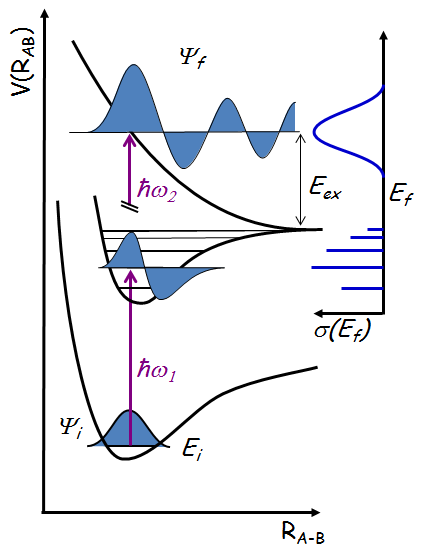
\includegraphics[scale=0.5]{Absorpce.png}
\caption{Absorpční spektrum molekul.}
\label{obr:Absorpce}
\end{figure}

Existuje ještě jedna cesta umožnující vypočítat energie excitovaných stavů a intenzitu absorpce, aniž bychom přitom ale znali vlnovou funkci excitovaného stavu. V~kapitole \ref{kap:vlastnosti} jsme diskutovali veličinu nazvanou polarizovatelnost. Ta nám říká, jak moc je molekula citlivá na vnější elektrické pole. Vnější elektrické pole může být ale i časově proměnné, v~případě světla o~frekvenci $\nu$ se intenzita elektrického pole mění harmonicky dle vztahu

\begin{equation}
\vec{E}(t) = \vec{E_0} \sin (2 \pi \nu t).
\label{rov:Ex-6}
\end{equation}

Můžeme se nyní tázat, jak je molekula citlivá na elektrické pole o~této frekvenci. Získáme tak frekvenčně závislou polarizovatelnost molekuly $\alpha(\nu)$. Tato veličina prudce vzrůstá v~okamžiku, kdy je splněna rezonanční podmínka \eqref{rov:Ex-3}. V~principu tedy potřebujeme simulovat zkoumanou molekulu umístěnou do časově-proměnného pole, což vlastně odpovídá experimentu. K~tomu je potřeba časově-závislá Schr\"odingerova rovnice. V~praxi je možné pro málo intenzivní pole nutnost použití časově závislé Schr\"odingerovy rovnice obejít. Na tomto principu jsou založeny metody jako je velmi efektivní \textbf{metoda časově-závislé teorie funkcionálu hustoty} TD-DFT (z~angl. \textit{Time Dependent Density Functional Theory}), představující rozšíření DFT metod do oblasti excitovaných stavů nebo kupříkladu metoda EOM-CCSD (a angl. \textit{Equation of Motion Coupled Clusters Single and Double Excitations}), což je zase rozšířením metody spřažených klastrů do oblasti excitovaných stavů. 
   



\clearpage
\section{Mezimolekulové interakce}
Molekuly na sebe navzájem působí. Důkazů pro to máme více než dost. Pokud by se molekuly na větší vzdálenosti nepřitahovaly, byl by náš svět tvořen jen neposednými molekulami plynů. Naproti tomu pokud by se molekuly na krátkou vzdálenost neodpuzovaly, tak bychom se okamžitě propadli skrze podlahu a nebylo by nám zatěžko procházet zdí. O~povaze odpudivých a~přitažlivých sil začalo být poněkud více jasno od dob Johannese Diderika van der Waalse a jeho studia kondenzace plynů. Často proto nyní mluvíme o~van der waalsovských interakcích jako synonymu slabých mezimolekulových interakcí. Proč se částice přitahují a proč se odpuzují? A~jak silně na sebe částice působí? I~tuto informaci nám poskytne kvantová chemie.

Před tím, než si stručně něco řekneme o~\textit{ab initio} výpočtech slabých mezimolekulových interakcí si provedeme jejich stručnou inventuru. Rozdělíme si je na \uv{klasické} interakce a na interakce \uv{kvantové}.


\subsection{Klasické interakce}
Pod pojmem \uv{klasické} interakce máme na mysli působení vysvětlitelné elektrostatickými silami. Patří sem například

\begin{itemize} 

\item \textbf{Interakce náboj-náboj.} Dva ionty, jeden s~nábojem $q_i$ a druhý s~nábojem $q_j$ na sebe dle Coulombova zákona působí silou

\begin{equation}
E_{int} = \frac{1}{4 \pi \epsilon_0} \frac{q_i q_j}{r_{ij}}.
\label{rov:MS-1}
\end{equation}

\begin{figure} [htb]
\centering
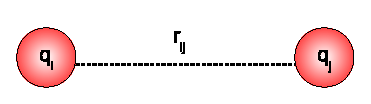
\includegraphics[scale=1]{nabojnaboj.eps}
\caption{Interakce náboj-náboj.}
\label{obr:Naboj-Naboj}
\end{figure}

\item \textbf{Interakce dipól-dipól.} Dvě molekuly s~nenulovým dipólovým momentem na sebe působí interakční energií

\begin{equation}
E_{int} = \frac{-1}{4 \pi \epsilon_0} \frac{\vec{\mu_i} \vec{\mu_j} [ 2 \cos \theta_i \cos \theta_j - \sin \theta_i \theta_j \cos \varphi]}{r_{ij}^3},
\label{rov:MS-2}
\end{equation}

\noindent kde $\vec{\mu}_i$ a $\vec{\mu}_j$ jsou dipólové momenty jednotlivých molekul. Všimněme si, že tato interakce vyhasíná se vzdáleností podstatně rychleji než interakce ion-ion. I~tento vzorec bychom při troše snahy odvodili z~Coulombova zákona. 

\begin{figure} [htb]
\centering
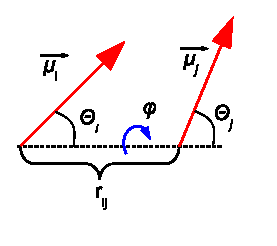
\includegraphics[scale=1]{dipoldipol.eps}
\caption{Interakce dipól-dipól.}
\label{obr:Dipol-Dipol}
\end{figure}

\item \textbf{Interakce dipól-indukovaný dipól.} I~zcela neutrální molekula bez jakýchkoliv elektrických momentů je přitahována k~molekule, která má náboj nebo třeba dipólový moment. V~neutrální molekule se totiž indukuje dipólový moment, který zpětně působí na indukující dipólový moment interakcí typu dipól-dipól. Interakční energie je pak dána jako


\begin{equation}
E_{int} = \frac{-1}{2(4 \pi \epsilon_0)^2} \frac{\vec{\mu_1}^2 \alpha_2 (1 + 3 \cos^2 \theta)}{r^6},
\label{rov:MS-3}
\end{equation}

\begin{figure} [htb]
\centering
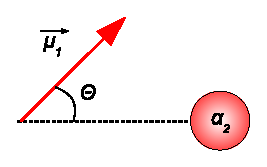
\includegraphics[scale=1]{indukovanydipol.eps}
\caption{Interakce dipól-indukovaný dipól.}
\label{obr:IndukovanyDipol}
\end{figure}

\noindent kde $\alpha_2$ je polarizovatelnost neutrální molekuly a $\mu_1$ je dipólový moment elektricky aktivní molekuly. 

\end{itemize}

Podobným způsobem bychom mohli naleznout vztahy pro interakce ion-dipól, dipól-kvad-rupól či třeba kvadrupól-indukovaný kvadrupól. Všechny tyto interakce lze snadno pochopit na základě fyziky 19. století, kvantové mechaniky zde netřeba. Na druhou stranu ani jedna z~těchto interakcí nevysvětluje, proč kondenzuje do kapalného či pevného stavu kupř. argon, který je prost všech elektrických momentů. Nevíme také pořád, proč nejsme schopni projít zdí.

\subsection{Kvantové interakce}   

Budeme uvažovat dva typy inherentně kvantových interakcí: (Pauliho) repulzi a disperzní interakci.

\begin{itemize} 

\item \textbf{Repulzní interakce.} Dva atomy helia přiblížené na velmi krátkou vzdálenost se začnou odpuzovat. Proč tomu tak je? Na první pohled by se mohlo zdát, že hlavně proto, že se do velké blízkosti dostávají dvě jádra helia, každé z~nich dvojnásobně nabité. To ale není vše, ba není to vůbec to hlavní: na druhou stranu si totiž elektrony vychutnávají přítomnost kladného náboje od druhého atomu. Hlavní problém je v~Pauliho vylučovacím principu. V~každém z~atomů helia se oba elektrony nachází v~1s orbitalu. Pokud se ale snažíme  ze dvou atomů udělat jenom jeden, tak čtyři elektrony se již ve stejném 1s orbitalu nacházet nemohou. Energie tak díky Pauliho repulzi roste. Tato repulze závisí na překryvu mezi příslušnými orbitaly a~můžeme ji proto dobře reprezentovat exponenciální funkcí
   

\begin{equation}
E_{int} = A e^{- \gamma r_{ij}}.
\label{rov:MS-4}
\end{equation}


\item \textbf{Disperzní interakce.} Jde o~přitažlivou interakci, která působí mezi libovolnými dvěma atomy. Někdy se mluví také o~Londonově interakci, dle v~Německu narozeného amerického fyzika Fritze Londona. Jaká je podstata této síly? Díky energii nulového bodu v~kvantové mechanice nikdy neutuchá pohyb. Elektron v~atomu tak neustále kmitá a v~každé chvíli má určitý okamžitý dipólový moment. Tento dipólový moment ale indukuje dipólový moment v~sousedním atomu a oba atomy se tak přitahují interakcí okamžitý dipól-indukovaný dipól. Fritz London odvodil pro tuto interakci přibližný vztah

\begin{equation}
E_{int} \approx \frac{-3}{2 (4 \pi \epsilon_0)^2} \frac{I_A I_B}{I_A + I_B} \frac{\alpha_A \alpha_B}{r_{ij}^6},
\label{rov:MS-5}
\end{equation}

\noindent 
kde $I_A$ a $I_B$ jsou ionizační energie na sebe působících molekul A~a B a~analogicky $\alpha_A$ a~$\alpha_B$ jsou polarizovatelnosti těchto molekul.  
\end{itemize}

\subsection{\textit{Ab initio} výpočty slabých mezimolekulových interakcí}

V~minulých oddílech jsme si představily celou řadu vztahů, které popisují jednotlivé typy slabých mezimolekulových interakcí. Na první pohled tak vše vypadá růžově. Stačí nám vypočítat si metodami kvantové chemie vlastnosti jednotlivých molekul, tedy jejich náboj, dipólový případně vyšší momenty, polarizovatelnost či ionizační energii a poté s~použitím vztahů \eqref{rov:MS-1} až \eqref{rov:MS-5} snadno dopočítáme, jak na sebe molekuly působí. Bohužel pro složitější molekuly takto postupovat nelze a je třeba interakční energii pro vzájemné působení molekul vypočítat přímo. Popíšeme si nyní dvě možné strategie takovéhoto výpočtu.


\subsubsection{Poruchový výpočet: Symetricky adaptovaná poruchová teorie}

Slabé mezimolekulové interakce v~sobě obsahují ono návodné adjektivum \uv{slabé}. Interakce mezi dvěma molekulami tedy může být nahlížena jako malá porucha při pohybu elektronů v~jednotlivých atomech. Podívejme se na jednoduchý případ dvou atomů helia v~určité vzdálenosti.


\begin{figure} [htb]
\centering
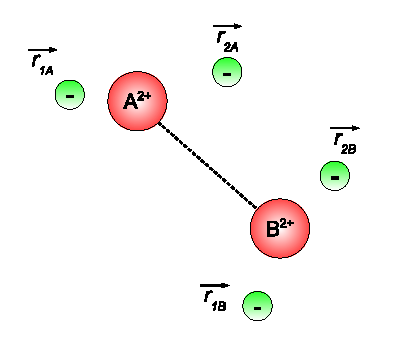
\includegraphics[scale=1]{atomhelia.eps}
\caption{Geometrie atomu helia.}
\label{obr:AtomHelia}
\end{figure}


Elektronový hamiltonián můžeme v~atomových jednotkách zapsat jako


\begin{eqnarray}
\hat{H}_{el} &=&  \underbrace{- \frac{1}{2} (\Delta_{1A} + \Delta_{2A}) + \left( \frac{1}{\vert \vec{r}_{1A} - \vec{r}_{2A} \vert} - \frac{2}{\vert \vec{r}_{1A} - \vec{R_A}\vert} - \frac{2}{\vert \vec{r}_{2A} - \vec{R_A} \vert} \right)}_{\hat{H}_A} \nonumber \\
&-& \underbrace{\frac{1}{2} (\Delta_{1B} + \Delta_{2B}) + \left( \frac{1}{\vert \vec{r}_{1B} - \vec{r}_{2B} \vert} - \frac{2}{\vert \vec{r}_{1B} - \vec{R_B}\vert} - \frac{2}{\vert \vec{r}_{2B} - \vec{R_B} \vert} \right)}_{\hat{H}_B} \nonumber \\
&+&  \bigg( \frac{4}{\vert \vec{R_A} - \vec{R_B}\vert} + \frac{1}{\vert \vec{r}_{1A} - \vec{r}_{1B} \vert} + \frac{1}{\vert \vec{r}_{1A} - \vec{r}_{2B}\vert} + \frac{1}{\vert \vec{r}_{2A} - \vec{r}_{1B} \vert} + \frac{1}{\vert \vec{r}_{2A} - \vec{r}_{2B} \vert} \nonumber \\
&-&  \frac{2}{\vert \vec{r}_{1A} - \vec{R_B} \vert} - \frac{2}{\vert \vec{r}_{2A} - \vec{R_B} \vert} - \frac{2}{\vert \vec{r}_{1B} - \vec{R_A} \vert} - \frac{2}{\vert \vec{r}_{2B} - \vec{R_A} \vert} \bigg),
\label{rov:MS-6}
\end{eqnarray}

\noindent což lze rozepsat jako 

\begin{equation}
\hat{H}_{el} = \underbrace{\hat{H}_A + \hat{H}_B}_{\hat{H}_A^{(0)}} + \hat{H}_{AB}.
\label{rov:MS-7}
\end{equation}

\noindent Řešení rovnice 

\begin{equation}
\hat{H}_{A}^{(0)} \psi_{el}^{(0)} = E_{el}^{(0)} \psi_{el}^{(0)},
\label{rov:MS-8}
\end{equation}

\noindent kde 

\begin{equation}
\hat{H}_A^{(0)} = \hat{H}_A + \hat{H}_B
\label{rov:MS-9}
\end{equation}


\noindent snadno získáme metodou separace proměnných

\begin{equation}
\psi_{el}^{(0)} = \psi_A (\vec{r}_{1A}, \vec{r}_{2A}) \psi_B (\vec{r}_{1B},\vec{r}_{2B}),
\label{rov:MS-10}
\end{equation}


\noindent kde $\psi_A$ je vlnová funkce prvního atomu helia a $\psi_B$ je vlnová funkce druhého atomu helia. Interakční energii pak můžeme vypočítat v~rámci poruchové teorie jako


\begin{equation}
E^{(1)} = \int \psi_{el}^{(0)} \hat{H}_{AB} \psi_{el}^{(0)} \mathrm{d} \vec{r}_{1A} \mathrm{d} \vec{r}_{2A} \mathrm{d} \vec{r}_{1B} \mathrm{d} \vec{r}_{2B}.
\label{rov:MS-11}
\end{equation}


Vypadá to vše jednoduše, ale bohužel je tam zádrhel. Vlnová funkce \eqref{rov:MS-10} není antisymetrická vůči záměně elektronů mezi oběma atomy helia. Je třeba celý postup upravit, mluvíme pak o~symetricky adaptované poruchové teorii (SAPT, z~angl. \textit{Symmetry Adapted Perturbation Theory}). 


\subsubsection{Supramolekulární přístup}
V~rámci supramolekulárního výpočtu vyjádříme interakční energii jako rozdíl energie molekulárního komplexu $E_{AB}$ a energií jednotlivých komponent $E_A$ a $E_B$

\begin{equation}
E_{int} = E_{AB} - E_A - E_B.
\label{rov:MS-12}
\end{equation}


Přístup je to velmi přímočarý a zdá se, že nemůže zklamat. Má ale své problémy. Energie molekul nikdy nepočítáme přesně, ale vždy v~rámci nějaké přibližné metody. I~ty nejnáročnější přístupy poskytují pro realistické systémy hodnoty energií, které se v~absolutní hodnotě od skutečné hodnoty značně liší. Naštěstí větší část chyby se při výpočtu komplexu a komponent vzájemně vyruší, v~chemii nám totiž většinou jde pouze o~rozdíly energií. V~případě slabých mezimolekulových sil nicméně počítáme velmi malou energii jako rozdíl velikých (a skoro stejných) čísel, \uv{snažíme se zjistit hmotnost kapitána jako rozdíl hmotnosti kapitána s~parníkem a~samotného parníku}. V~takovém případě se začnou uplatňovat i jinak zanedbatelné efekty.

Jedním z~problémů je tzv. superpoziční chyba. Jde o~následující problém. Pokud provádíme variační výpočet, tak  víme, že čím větší báze, tím nižší energie. Jestliže nyní provádíme výpočet molekulového komplexu A...B, tak molekula A~v~komplexu může při výpočtu využít i bázových funkcí poskytnutých molekulou B. Dojde ke snížení energie, které není dáno fyzikální interakcí, ale jde toliko o~matematický artefakt. Komplex se pak jeví stabilnější než ve skutečnosti je. Tento defekt odstraňujeme tzv. \textit{counterpoise} korekcí. Interakční energii komplexu vyjádříme jako 

\begin{equation}
E_{int} = E_{AB} - E_{A,[B]} - E_{B,[A]},
\label{rov:MS-13}
\end{equation}

\noindent kde $E_{A,{[B]}}$ je energie atomu A~vypočítaná za přítomnosti báze atomu B a $E_{B,{[A]}}$ je energie atomu B vypočítaná za přítomnosti báze atomu A. Vyvážíme tak neférovou výhodu, které se dostalo atomům A a B v~komplexu A...B.


\section{Výpočty v kondenzované fázi}
Skoro všechna zajímavá chemie se odehrává v~kondenzované fázi. Naproti tomu v~našem výkladů jsem se doposud zabývali výhradně výpočty prováděnými v~plynné fázi. V~mnoha případech to nijak zvlášť nevadí. Reakce neutrálních molekul nejsou příliš ovlivněny prostředím a výpočet provedený v~plynné fázi tak představuje dobré přiblížení pro situaci v~roztoku.
Děje, ve kterých vystupují ionty jsou ale solvatací ovlivněny zcela zásadně. Tak například molekula NaCl se v~plynné fázi určitě neoddělí na ionty, zatímco ve vodě je disociace v~ionty zcela tuctovou podívanou.
Kvalitní popis solvatace je proto jedním z~ústředních problémů současné výpočetní chemie. V~tomto textu jenom velmi stručným způsobem načrtneme možnosti, které se před námi otevírají, případného zájemce o~hlubší vhled odkazujeme na kteroukoliv z~velké řady publikací a kompendií věnovaných výpočetní chemii, kupříkladu na práci Cramerovu.\footnote{C. J. Cramer, Essentials of Computational Chemistry. Theories and Models, 2nd edition. Wiley, 2004.} Nyní tedy pouze stručný přehled:

\begin{itemize}

\item \textbf{Mikrosolvatace.} V~rámci tohoto přístupu jednoduše obklopíme molekulu molekulami rozpouštědla a pro celý tento systém pak počítáme vlastnosti (například energii). Jde o~přímočarou cestu k~zahrnutí solvatačních efektů, nicméně nikoliv o~cestu příliš praktickou. Malé agregáty mají totiž jen málo co společného s~kondenzovanou fází a konvergence vlastností molekul s~velikosti použitého klastru je velmi pomalá. Naproti tomu výpočetní náročnost kvantově-chemických metod velmi silně roste s~velikostí systému. Ačkoliv dnes již je možné za určitých okolností provádět kvantové výpočty i pro stovky molekul, jde pořád o~mimořádně nákladný podnik. Jinou potíží je skutečnost, že systém s~větším počtem solvatujících molekul vykazuje celou řadu energetických minim o~přibližně stejné energii a výpočet s~jediným z~těchto minim není příliš smysluplný. Je proto třeba použít metod molekulových simulací, kupříkladu metodu molekulové dynamiky nebo metodu Monte Carlo, pomocí kterých můžeme simulovat statistické soubory molekul. Při výpočtech na \textit{ab initio} úrovni je to ovšem výpočetně dosti náročné.

\begin{figure} [htb]
\centering
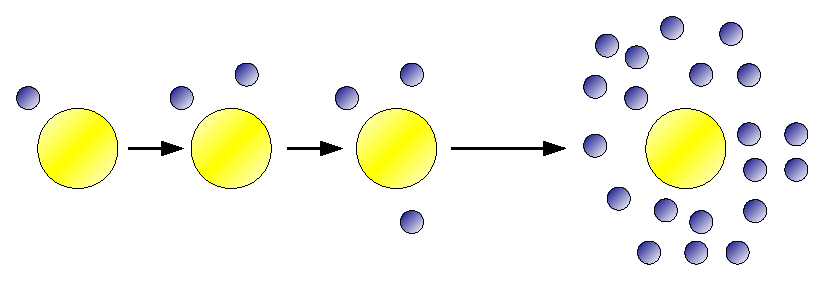
\includegraphics[scale=1]{Mikrosolvatace.eps}
\caption{Mikrosolvatace.}
\label{Mikrosolvatace}
\end{figure}

\item \textbf{QM/MM metody.} V~rámci tohoto přístupu studujeme část systému metodami kvantové chemie a část jednoduššími přístupy, s~použitím empirických potenciálů. Empirické potenciály popisují molekuly pomocí různých empirických vazebných příspěvku a interakce mezi molekulami je pak realizována elektrostatickými, repulzními a disperzními příspěvky.\footnote{Empirickým potenciálům se v~tomto textu nevěnujeme, čtenáře zde odkazujeme kupř. na text Petra Bouře na http://hanicka.uochb.cas.cz/~bour/prednaska/prednaska.htm}  Na kvantové úrovni řešíme většinou pouze ty nejdůležitější části systému, například aktivní centrum enzymu, okolí či roztok pak popisujeme metodami empirickými. hamiltonián je pak dán jako


\begin{equation}
\hat{H} = \hat{H}_{QN} + \hat{H}_{MM} + \hat{H}_{QM/MM},
\label{rov:Sol-1}
\end{equation}

\noindent kde $\hat{H}_{QM}$ je hamiltonián pro molekulu rozpuštěné látky počítaný na kvantově-chemické úrovni, $\hat{H}_{MM}$ představuje empirický potenciál a $\hat{H}_{QM/MM}$ popisuje interakci mezi oběma částmi. V~nejběžnějším případě můžeme psát

\begin{equation}
\hat{H}_{QM/MM} = - \sum_i \sum_M \frac{q_M}{r_{iM}} + \sum_{\alpha} \sum_M \frac{Z_{\alpha} q_M}{R_{\alpha M}} + \sum_{\alpha} \sum_M 4 \epsilon_{\alpha M} \left[ \left( \frac{\sigma_{\alpha M}}{R_{\alpha M}} \right)^{12} - \left( \frac{\sigma_{\alpha M}}{R_{\alpha M}} \right)^6 \right],
\label{rov:Sol-2}
\end{equation}

\noindent
kde $q_M$ je náboj molekulárně-mechanického (MM) atomu $M$, $Z_{\alpha}$ je nábojové číslo kvan\-tově-mechanického (QM) atomu $\alpha$ a $\epsilon_{\alpha M}$ a $R_{\alpha M}$ jsou parametry Lennard-Jonesova potenciálu popisující repulzní a disperzní síly mezi kvantově-mechanickým atomem $\alpha$ a~mole\-ku\-lárně-mechanickými atomy $M$. Elektrony jdou označeny indexem $i$. Elektrony i~jádra rozpuštěné látky popsané na QM úrovni tedy \uv{cítí} parciální náboje MM atomů a k~tomu přidáváme repulzi a disperzní přitahování mezi QM a MM atomy. 

Díky QM/MM přístupu je tak možné studovat i velmi rozsáhlé systémy. O~důležitosti QM/MM metod svědčí i Nobelova cena za rok 2013 udělená právě za výzkumy v~tomto směru. 

\begin{figure} [htb]
\centering
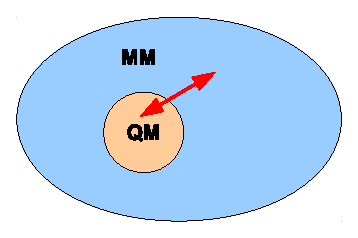
\includegraphics[scale=1]{QM_MM.eps}
\caption{Schéma strategie QM/MM.}
\label{obr:QM_MM}
\end{figure}


\item \textbf{Implicitní modely.} Představme si, že chceme vypočítat energii určitého iontu v~roztoku. Pro jednoduchost uvažujme ion kulovitého tvaru. Můžeme vypočítat energii iontu v~plynné fázi a připočítat solvatační energii. Ta je v~nejjednodušším případě dána Bornovou rovnicí, kdy solvatační energii vypočítáme z~rovnic klasické elektrostatiky jako rozdíl práce nutné k~nabití iontu ve vakuu a v~prostředí o~relativní permitivitě $\epsilon_r$


\begin{equation}
\Delta G_{sol} = - \frac{Z_i e^2}{8 \pi \epsilon_0 r_i} \left(1- \frac{1}{\epsilon_r} \right),
\label{rov:Sol-3}
\end{equation}

\noindent kde $r_i$ je poloměr příslušného iontu, $Z_i$ je nábojové číslo iontu a $\epsilon_0$  je permitivita vakua. Jde o~velmi přímočarou opravu na vliv solvatace, která ovšem nebere v~potaz některé složky solvatační energie. Tak kupříkladu zanedbává tzv. kavitační energii, tj. energii nutnou na vytvoření kavity, do které příslušný ion umístíme. Tuto veličinu můžeme odhadnout například z~hodnot povrchového napětí kapaliny, ve kterém molekulu solvatujeme. 

\begin{figure} [H]
\centering
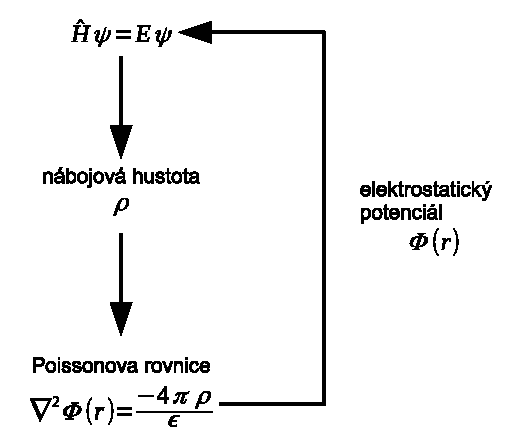
\includegraphics[scale=1]{SCRF_kolecko.eps}
\caption{Nástin algoritmu SCRF.}
\label{SCRF}
\end{figure}

\noindent Kromě toho předpokládáme, že elektronová struktura není solvatací ovlivněna. To ale není nutně splněno. Ion totiž polarizuje rozpouštědlo, které ho obklopuje, které ale zpětně působí svým polem na solvatovaný ion. Vytváří se tzv. reakční pole, ve kterém je ion umístěn. Korektní postup tak spočívá v~tom, že řešením Schr\"odingerovy rovnice vypočítáme elektrické pole generované naším iontem, v~tomto poli řešíme elektrostatické rovnice pro okolní roztok, získáme ono reakční pole a znovu znovu opakujeme celý výpočet, dokud se již vlnová funkce ani reakční pole nemění (SCRF, z~angl. \textit{Self Consistent Reaction Field}). Tento přístup je pouze o~málo náročnější než výpočet ve vakuu a bývá proto často používán. Na druhou stranu je třeba být obezřetný, neboť model má svá dobře známá omezení.        

     


\end{itemize}

\clearpage
\section{Relativistické efekty}
Dvacáté století přineslo ve fyzice dvě zásadní revoluce: speciální teorie relativity přinesla novou mechaniku pro rychle se pohybující částice a~kvantová teorie pak novou mechaniku pro oblast mikrosvěta. Co ale dělat s~rychle se pohybujícími objekty mikrosvěta? O~tom nás zpravuje relativistická kvantová mechanika. 

V kapitole \ref{kap:abinitio} jsme se seznámili s~různými metodami, kterými můžeme řešit Schr\"odingerovu rovnici. Mohli jsme tak nabýt dojmu, že kupříkladu metoda úplné konfigurační interakce představuje svatý grál kvantové chemie, který nás dovede rovnou k \uv{pravdě}. Ve skutečnosti ani energie a~vlnová funkce vypočítaná metodou konfigurační interakce s nekonečnou jedno-elektronovou bází neposkytne přesnou hodnotu energie. Základním problémem je zanedbání relativistických efektů. Dle teorie relativity základní parametr každé hmotné částice, totiž její hmotnost $m$, závisí na rychlosti pohybu této částice

\begin{equation}
m = \frac{m_0}{\sqrt{1 - \frac{v^2}{c^2}}},
\label{rov:Rel-1}
\end{equation}

\noindent kde $m_0$ je klidová hmotnost částice, $v$ její rychlost a  $c$ je rychlost světla ve vakuu. Měli bychom se v~chemii vůbec trápit relativistickými efekty? Odpověď nám naznačí následující příklad.

\begin{priklad}
\textbf{Zadání:} Odhadněte hmotnost $m$ elektronu v~atomu vodíku a v~1s orbitalu atomu rtuti.\\[0.1cm]
\textbf{Řešení:} K~odhadu použijeme výraz pro rychlost z~Bohrovy teorie atomů vodíkového typu

\begin{displaymath}
v = \frac{Z}{n} \alpha c,
\end{displaymath}

\noindent kde $Z$ je nábojové číslo jádra, $n$ je hlavní kvantové číslo, $c$ je rychlost světla ve vakuu a~$\alpha$ je tzv. konstanta jemné struktury mající hodnotu $1/137$. V~případě rtuti jde jen o~hrubý odhad, jádro rtuti bude stíněno i zbylými ostatními elektrony. V~případě 1s orbitalu půjde ale o~stínění nevýznamné. Pro vodík tak dostáváme rychlost

\begin{displaymath}
v = \frac{c}{137} \Rightarrow m \doteq m_0 \quad (1{,}000026 \cdot m_0)
\end{displaymath}

\noindent a pro rtuť s~$Z=80$

\begin{displaymath}
v \doteq \frac{80}{137} c \Rightarrow m \doteq 1{,}23 \cdot m_0.
\end{displaymath}

\noindent Takže zatímco u~atomu vodíku se hmotnost téměř nezmění, u~těžších atomů už musíme brát relativistické efekty nejspíše vážně. Změna hmotnosti elektronu totiž jistě povede k~odlišnému chování jednotlivých orbitalů.
\end{priklad}

Pro popis relativistických efektů je nutné vytvořit rovnici, která je v~souladu jak s~postuláty kvantové mechaniky, tak s~teorií relativity. V~klasické, nerelativistické mechanice je energie volné částice dána jako

\begin{equation}
E = \frac{p^2}{2m},
\label{rov:Rel-2}
\end{equation}
  
\noindent čemuž odpovídá hamiltonián 

\begin{equation}
\hat{H} = - \frac{\hbar^2}{2m} \Delta
\label{rov:Rel-3}
\end{equation}

\noindent a časově-závislá Schr\"odingerova rovnice 

\begin{equation}
i \hbar \frac{\partial \psi}{\partial t} = \hat{H} \psi.
\label{rov:Rel-4}
\end{equation}

Mohli bychom být v~pokušení vyjít nyní s~relativistického výrazu pro energii

\begin{equation}
E^2 = p^2 c^2 + m_0^2 c^4
\label{rov:Rel-5}
\end{equation}

\noindent a s~použitím stejných pravidel ($E$ nahradíme $E \rightarrow i \hbar \frac{\partial}{\partial t}$ a $p$ nahradíme $\vec{p}_x \rightarrow i \hbar \frac{\partial}{\partial x}$) bychom získali tzv. Kleinovu-Gordonovu rovnici

\begin{equation}
\frac{1}{c^2} \frac{\partial^2 \psi}{\partial t^2} - \Delta \psi + \frac{m_0^2 c^2}{\hbar^2} \psi = 0.
\label{rov:Rel-6}
\end{equation}

Bohužel se ukazuje, že v~této rovnici se nezachovává počet částic. Není ji možné použít pro popis fermionů (hodí se však pro popis bosonů). Správnou rovnici pro elektron formuloval Paul Dirac. Vyšel opět z~rovnice \eqref{rov:Rel-5} a svou geniální intuicí dospěl k~závěru, že elektron je popsán nikoliv jednou vlnovou funkcí, ale rovnou uspořádanou čtveřicí vlnových funkcí

\begin{equation}
\psi = 
\begin{pmatrix}
\psi_1 \\
\psi_2 \\
\psi_3 \\
\psi_4
\end{pmatrix},
\label{rov:Rel-7}
\end{equation}

\noindent které se pak řídí \textbf{Diracovou rovnicí} formálně připomínající rovnici Schr\"odingerovu pro atom vodíku

\begin{equation}
i \hbar \frac{\partial \psi}{\partial t} = \hat{h} \psi,
\label{rov:Rel-8}
\end{equation}
kde
\begin{equation}
\hat{h} = c \cdot \alpha \cdot \hat{p} + \beta \cdot c^2 + V_N,
\label{rov:Rel-9}
\end{equation}

\noindent kde $\alpha$ a $\beta$ představují matice rozměru $4 \times 4$. Jednotlivé komponenty vlnové funkce odpovídají elektronu se spinem $\alpha$ a $\beta$ a pozitronu se spinem $\alpha$ a $\beta$. Dirac tak ukázal, že požadavek na kompatibilitu mezi kvantovou mechanikou a teorií relativity vede automaticky k~elektronovému spinu a také k~existenci antičástic.  
    
  

\subsection{Relativistické efekty v~chemii}

Relativistické efekty můžeme rozdělit do dvou základních skupin. 

\begin{itemize} 

\item \textbf{Skalární relativistické efekty}. Jde o~efekty spojené s~rozdílným relativistickým výrazem pro energii a tedy s~rozdílnou hmotností elektronu. Nejde tedy o~jevy, které by souvisely s~tím, že vlnová funkce má čtyři komponenty. 

Elektron má díky relativitě větší hmotnost. Můžeme tak očekávat, že se díky tomu elektron bude chovat klasičtěji, bude se pohybovat blíže k~atomovému jádru. V~případě s~a p orbitalů tak bude docházet ke kontrakci orbitalů\footnote{Tento pojem nelze zaměňovat s~relativistickou kontrakcí délek.}. Díky kontrakci s~a p orbitalů je ale na druhou stranu jádro lépe stíněno. Elektrony v~d a f orbitalech proto pociťují menší efektivní náboj a díky tomu dochází k~jejich expanzi. Tyto jevy mají rozličné projevy v~chemii. Například v~případě zlata dochází ke stabilizaci elektronů v~6s orbitalu a k~ionizaci dochází z~5d orbitalů. Vznikají tak trivalentní nebo pentavalentní ionty zlata. Díky relativistickým efektům jsou také stabilnější vyšší oxidační stavy kovů, takže může existovat kupříkladu i ion IrO$_4^+$, který obsahuje iridium v~formálním oxidačním stavu +IX. Dochází také k~určitému zkrácení vazebné délky, částečně relativistickým efektem je i~lanthanoidová kontrakce. Jedině díky relativitě můžeme využívat v~automobilech olověných akumulátorů. Olovo má elektronovou konfiguraci 6s$^2$6p$^2$. Elektrony v~těchto orbitalech jsou relativisticky stabilizované, díky čemuž má olovo v~oxidačním stupni +IV vyšší energii. To však v~důsledku vede k~větší změně Gibbsovy energie v~elektrodové reakci odehrávající se v~akumulátorech

\begin{equation}
\mbox{Pb}(s) + \mbox{PbO}_2(s) + 2 \mbox{H}_2\mbox{SO}_4 (aq) \rightarrow 2 \mbox{PbSO}_4 (s) + 2 \mbox{H}_2\mbox{O} (l).
\label{rov:Rel-10}
\end{equation}

\noindent Bez zahrnutí relativistických efektů by zlato nebylo žluté a rtuť by nebyla kapalná. S~relativitou se zkrátka v~chemii potkáváme docela často. 

\item \textbf{Relativistické efekty spojené se spinem}. Zde máme na mysli především tzv. spin-orbitální interakci, o~které již byla řeč v~kapitole~\ref{kap:viceelektron}. Tento efekt se projeví korekcí k~nerelativistickému hamiltoniánu

\begin{equation}
\hat{H}_{SO} = - \xi \cdot \hat{\vec{L}} \hat{\vec{S}},
\label{rov:Rel-11}
\end{equation}

\noindent
kde $\vec{L}$ je orbitální moment a $\vec{S}$ je spinový moment elektronu. Spin-orbitální interakce se opět uplatňuje zejména pro těžší atomy. Způsobuje rozštěpení mezi energetickými hladinami, pro těžší prvky často značné.

\end{itemize}

\subsection{Kvantově-chemické výpočty relativistických efektů}

Při výpočtech zahrnujících efekty spojené s~teorií relativity bychom mohli vyjít z~Diracovy rovnice. Ta ovšem popisuje pohyb pouze jednoho elektronu. Je proto třeba přidat člen popisující interakci mezi elektrony. Mohli bychom k~Diracovu členu přidat coulombické odpuzování mezi elektrony. Takovýto přístup ale není relativisticky plně konzistentní. Mimo jiné předpokládáme, že k~interakci mezi elektrony dochází okamžitě, což při konečné rychlosti světla není pravda. Lepším přístupem je konstrukce tzv. Diracova-Coulombova-Breitova hamiltoniánu

\begin{equation}
\hat{H} = \sum_i \hat{h}_i + \sum_{i<j} \hat{h}_{ij},
\label{rov:Rel-12}
\end{equation}

\noindent kde $\hat{h}_i$ je jednočásticový Diracův hamiltoninán \eqref{rov:Rel-9} a dvou-částicový člen je dán jako součet coulombického a Breitova členu v~atomových jednotkách

\begin{equation}
\hat{h}_{ij} = \frac{1}{r_{ij}} - \frac{1}{2 r_{ij}} \left[ \alpha_i \alpha_j + \frac{(\alpha_i \vec{r}_{ij})(\alpha_j \vec{r}_{ij})}{r_{ij}^2} \right].
\label{rov:Rel-13}
\end{equation}

Rovnici tohoto typu pro čtyř-komponentovou vlnovou funkci můžeme dále zjednodušovat. Je snadné se zbavit dvou komponent popisujících pozitrony. Často se také používají ryze rovnice popisující pouze skalární relativistické efekty, například v~rámci přístupu ZORA (z angl. \textit{Zero Order Relativistic Approximation}).

Pragmatickou cestou k~zahrnutí relativistických efektů je použití tzv. efektivních relativistických pseudopotenciálů pro vnitřní elektrony (ECP, z~angl. \textit{Effective Core Pseudopotential}). Relativistické příspěvky jsou totiž významné zejména pro elektrony vnitřních slupek, valenční elektrony se pohybují daleko pomaleji, neboť jejich interakce s~atomovými jádry je již hodně stíněna právě vnitřními elektrony. Chemika ale vnitřní elektrony obvykle mnoho nezajímají, chemické reakce představují děje ve valenční sféře. Můžeme proto vnitřní elektrony nahradit vhodně zvoleným potenciálem, který simuluje vnitřní elektrony. Tento potenciál si jednou pro vždy nastavíme pro daný atom s~pomocí plně relativistického výpočtu a pak jej můžeme volně použít pro libovolné molekuly, jejíž je daný atom součástí. Získáme tak kvalitnější výsledek a navíc jako bonus je výpočet časově méně náročný, neboť vnitřní elektrony již do výpočtů nezahrnujeme.         
  
Oblast relativistické kvantové chemie představuje intenzivní předmět současného výzkumu a není v~možnostech tohoto textu se této otázce do detailu věnovat. Zájemce můžeme odkázat na dva výtečné přehledné články pod Pekky Pyyk\"oho.\footnote{P. Pykk\"o, \textit{Relativistic Effects in Chemistry: More Common Than You Thought.} Annu. Rev. Phys. Chem. 2012, 63, 45-64 a P. Pykk\"o, JP Desclaux, \textit{Relativity and the Periodic Systems of Elements} Acc. Chem. Res. 1979, 51, 276-281.}



      

   




 




      

      





%%% Vytvoření seznamu literatury.
%\newpage
%\addcontentsline{toc}{section}{BIBLIOGRAPHY}
%\bibliography{literatura} % if you have multiple bib files, never put space after comma

%%% Přílohy.
%\newpage
%\section*{A}
%\addcontentsline{toc}{section}{APPENDICES}
%\appendix

%\newpage
%\section*{Seznam zkratek}
%\bigskip
%\begin{tabular}{ll}
%\bf HF & Hartreeho-Fockova metoda \\
%\bf PES & povrch potenciální energie (Potential Energy Surface)\\	
%\end{tabular}

\end{document}
